\documentclass[a4paper,12pt]{book}
\usepackage[a4paper, margin=1in]{geometry}
\setlength{\parindent}{0cm}
\setlength{\parskip}{1\baselineskip}

\setcounter{secnumdepth}{4}
\usepackage{amsthm}
\usepackage{aliascnt}
\usepackage{amsmath,amssymb,amsfonts}
\usepackage{hyperref}
\usepackage[shortlabels]{enumitem}


\RequirePackage[dvipsnames,usenames]{xcolor}
\usepackage{mathtools}
%\usepackage{showkeys}
\usepackage[abbrev,alphabetic]{amsrefs}
\usepackage[all]{xy}
\usepackage{tikz}
\usepackage{tikz-cd}
\usepackage{systeme}

\usepackage{tikz-cd}

\newcommand{\basetheorem}[3]{
	\newtheorem{#1}{#2}[#3]
	\newtheorem*{#1*}{#2}
	\expandafter\def\csname #1autorefname\endcsname{#2}
}
\newcommand{\maketheorem}[3]{
	\newaliascnt{#1}{#3}
	\newtheorem{#1}[#1]{#2}
	\aliascntresetthe{#1}
	\expandafter\def\csname #1autorefname\endcsname{#2}
	\newtheorem{#1*}{#2}
}

%\theoremstyle{plain}
\basetheorem{theorem}{Theorem}{section}
\maketheorem{definition}{Definition}{theorem}
\maketheorem{lemma}{Lemma}{theorem}
\maketheorem{example}{Example}{theorem}
\maketheorem{corollary}{Corollary}{theorem}
\maketheorem{conjecture}{Conjecture}{theorem}
\maketheorem{proposition}{Proposition}{theorem}
\maketheorem{question}{Question}{theorem}
\maketheorem{remark}{Remark}{theorem}
%\basetheorem{theorem*}{Theorem}

\basetheorem{theo}{Theorem}{}
\newcounter{tmp}

\setcounter{tmp}{\value{theo}}% store current value of theorem counter
\setcounter{theo}{0} %assign desired value to theorem counter
\renewcommand\thetheo{\Alph{theo}}% locally redefine the representation of the theorem counter


\makeatletter
\newcommand{\newreptheorem}[2]{\newtheorem*{rep@#1}{\rep@title}\newenvironment{rep#1}[1]{\def\rep@title{#2 \ref*{##1}}\begin{rep@#1}}{\end{rep@#1}}}
\makeatother
\makeatletter
\@namedef{subjclassname@2020}{%
	\textup{2020} Mathematics Subject Classification}
\makeatother


%\newreptheorem{theorem}{Theorem}

%begin: Iacopo-defined newcommands
\DeclareMathOperator{\Spec}{Spec}
\DeclareMathOperator{\Proj}{Proj}
\newcommand{\bP}{\mathbb{P}}
\newcommand{\bR}{\mathbb{R}}
\newcommand{\bQ}{\mathbb{Q}}
\newcommand{\bN}{\mathbb{N}}
\newcommand{\bZ}{\mathbb{Z}}
\newcommand{\fB}{\mathbf{B}}
\newcommand{\fM}{\mathbf{M}}
\newcommand{\charac}{\textup{char }}
\newcommand{\id}{\textup{id}}
\newcommand{\Alb}{\textup{Alb}}
\newcommand{\cO}{\mathcal{O}}
\newcommand{\red}{\textup{red}}
\newcommand{\lct}{\textup{lct}}
\newcommand{\exc}{\textup{Ex}}
\newcommand{\coeff}{\textup{coeff}}
\newcommand{\cent}{\textup{centre}}
\newcommand{\codim}{\textup{codim}}
\newcommand{\textoverline}[1]{$\overline{\mbox{#1}}$}
\newcommand{\rk}{\textup{rk}}
\newcommand{\WDiv}{\textup{WDiv}}
%end: Iacopo-defined newcommands


\newcommand{\A}{\mathcal{A}}
\newcommand{\B}{\mathcal{B}}
\newcommand{\C}{\mathcal{C}}
\newcommand{\D}{\Delta}
\newcommand{\Vol}{\text{Vol}}
\newcommand{\Sing}{\text{Sing}}
\newcommand{\E}{\mathcal{E}}
\newcommand{\F}{\mathcal{F}}
\newcommand{\PP}{\mathcal{P}}
\newcommand{\HH}{\mathcal{H}}
\newcommand{\SB}{\mathbf{SB}}
\newcommand{\BB}{\mathbf{B}}
\newcommand{\BS}{\mathbf{B}_{+}}
\newcommand{\disc}{\text{Discrepancy}}


\newcommand{\ta}[1]{\mathcal{A}^{\leq #1}}
\newcommand{\at}[1]{\mathcal{A}^{\geq #1}}
\newcommand{\tb}[1]{\mathcal{B}^{\leq #1}}
\newcommand{\bt}[1]{\mathcal{B}^{\geq #1}}
\newcommand{\tc}[1]{\mathcal{C}^{\leq #1}}
\newcommand{\ct}[1]{\mathcal{C}^{\geq #1}}
\newcommand{\nklt}{\textup{Nklt}}
\newcommand{\Ht}[1]{H^{i}_{t}}
\newcommand{\orth}{^{\perp}}
\newcommand{\Hom}{\textup{Hom}}
\newcommand{\Fe}{F^{e}_{*}}
\newcommand{\Fn}[1]{F^{#1}_{*}}
\newcommand{\trip}{(R,\Delta, \alpha_{\bullet})}
\newcommand{\ai}{\alpha_{\bullet}}
\newcommand{\im}{\textup{Im}}
\newcommand{\ox}[1][X]{\mathcal{O}_{#1}}
\newcommand{\me}{M^{e}_{\Delta,a^{t}}}
\newcommand{\psim}{\sim_{\mathbb{Z}_{(p)}}}
\newcommand{\zp}{\mathbb{Z}_{(p)}}
\newcommand{\Xde}[1]{\mathcal{X}_{\delta,\epsilon,#1}}
\newcommand{\Pde}[1]{\mathcal{P}_{\delta,\epsilon,#1}}

%

\newtheorem{case}{Case}

\usepackage{xcolor}
\newcommand\myworries[1]{\textcolor{red}{#1}}

%\usepackage{subfiles}


\begin{document}
	\title{On the Minimal Model Program in positive and mixed characteristic}
	\author{Liam Stigant}
	\date{\today}
	\maketitle
	\chapter*{Abstract}
		
		This dissertation explores the Minimal Model Program (MMP) in positive and mixed characteristic in dimension three with a particular focus on outputs of the program. In purely positive characteristic we combine the program with a detailed study of conic bundles to prove a birational boundedness result. We show that given a suitable set of log Calabi-Yau varieties, we can construct a bounded family containing fibres birational to any member of the chosen set.
		
		For threefolds over a base of dimension at least one, we resolve the Abundance Conjecture for klt pairs in joint work with F. Bernasconi and I. Brivio. Showing in particular that every klt minimal model in mixed characteristic admits an Iitaka Fibration. This is then applied to prove an Invariance of Plurigenera result for suitable families of surfaces.
		
		Finally we consider outstanding questions around Mori fibrations in mixed characteristic. We show that every klt threefold MMP terminates and that any two Mori fibre space outputs of an MMP from the same starting pair are connected by a series of Sarkisov links. As part of this we prove a mixed characteristic Finiteness of Minimal Models result. While the proof is focused in dimension three, the arguments work in any generality given that the requisite MMP results are known.
		
	\tableofcontents
	
	\chapter*{Notation}
	
	\begin{itemize}
		\item Rings will often be denoted by $R$. They will always be excellent and admitting a dualising complex. We will often use the ring interchangeably with its spectrum, e.g. Let $R$ be a ring and $X \to R$ an $R$ scheme.
		\item If $R$ is a local ring we denote the residue field of the closed point by $k$ and the fraction field by $K$, unless otherwise stated.
		\item Schemes will always be excellent  and Noetherian. They will typically be denoted $W,X,Y,Z$. $S$ and $T$ are often used also, particularly for surfaces and the base of a pair respectively. They will essentially always be quasi-projective over a ring.
		\item If $X$ is a scheme over a local ring we often write $X_{k}$ for the closed fibre and $X_{K}$ for the generic fibre.
		\item If $X$ is an integral scheme we will write $K(X)$ for the fraction field
		\item A variety is a projective, integral scheme over a field.
		\item Given a scheme $X$ we write:
		\begin{itemize}
			\item $\text{WDiv}_{\mathbb{K}}(X)$ for the group of Weil divisors tensored by $\mathbb{K}=\mathbb{Z},\mathbb{Q}$ or $\mathbb{R}$ with the natural $\mathbb{K}$ module structure.
			\item $\text{Cl}_{\mathbb{K}}(X)$ for quotient of $\text{WDiv}_{\mathbb{K}}(X)$ of by the submodule generated by principle divisors
			\item $D \simeq_{\mathbb{K}}D'$ if $[D] =[D']$ inside $\text{Cl}_{\mathbb{K}}(X)$
		\end{itemize}
		\item Given a proper morphism of schemes $X \to T$:
		\begin{itemize}
			\item A curve will always be an integral, one dimensional scheme proper over a closed point of $T$.
			\item A $\mathbb{K}$ one cycle is formal sum of curves with coefficients in $\mathbb{K}=\mathbb{Z},\mathbb{Q}$ or $\mathbb{R}$. If no $\mathbb{K}$ is stated, we default to $\mathbb{R}$.
			\item $N_{1}(X/T)$ for the space of one cycles modulo numerical equivalence
			\item $N^{1}(X/T)$ for the space of $\mathbb{R}$-Cartier divisors modulo numerical equivalence
			\item $\overline{NE}(X/T)$ is the closure of the cone of effective one cycles. We sometimes call such one-cycles psuedo-effective, in analogy to divisors.
		\end{itemize}
		\item We say a proper morphism of schemes $f:X \to Y$ has (geometrically) connected fibres if $f_{*}\ox=\ox[Y]$. We may also say that $f$ is a contraction. When $\dim X > \dim Y$ such morphisms are also sometimes called fibrations. Note that despite the name, in characteristic $p>0$ this is a strictly stronger condition than the fibres being connected (take $f$ to be the Frobenius for example).
		\item Given a fibration $X \to T$ and a property $\mathcal{P}$ we say it is a family of $\mathcal{P}$ varieties if the fibre over each closed point $k$ is a $k$-variety with property $\mathcal{P}$.
		
		
		
	\end{itemize}
	
	\chapter{Introduction}

	Algebraic Geometry is the study of geometric shapes described as solutions to polynomials; or perhaps more generally the study geometric objects which are locally the spectra of rings.
	
	While this set of definitions offers a rich and fruitful area of study and a firm mathematical foundation from which to approach, they are not particularly useful methods of actually describing the objects of interest. One would not expect to see a variety given by some list of equations, nor as a list of rings and gluing information, except perhaps in the very simplest of examples.
	
	One of the key aims, then, of modern Birational Geometry is to provide a language and structure to better understand and describe the geometric objects appearing as part of the wider study of Algebraic Geometry. This is a role taken on directly by flagship conjectures like the Minimal Model Program (MMP), but is also supported by the myriad of ideas developed in the study of birational geometry. Notions like klt, for instance, which were developed to better understand the singularities appearing in the MMP have quickly spread throughout the larger field of Algebraic Geometry.
	
	We might summarise the key claim of the MMP as follows.
	
	\begin{conjecture*}
		Let $(X,\Delta)$ be a klt pair, projective over $T$. Then there is a $K_{X}+\Delta$ negative birational map of $T$ schemes $X \dashrightarrow X'$ inducing a pair $K_{X'}+\Delta'$ such that either
		
		\begin{enumerate}
			\item $K_{X'}+\Delta$ is nef; or
			\item There is a $K_{X'}+\Delta'$ negative contraction $X' \to Z$ of relative Picard rank $1$.
		\end{enumerate}
	\end{conjecture*}
	
	In the first case $X'$ is said to be a minimal model. In the latter we call $X' \to Z$ a Mori fibre space.
	
	At its most reductive, the MMP can be understood to claim that varieties can be built from three types of geometric objects - each with their own distinct properties. These are Fano, Calabi-Yau and General Type (or canonically polarised) varieties. For birational geometers it is natural to describe these in terms of their canonical bundle, these types of variety have $K_{X}$ negative (anti-ample), $K_{X}$ (numerically) trivial or $K_{X}$ positive (ample) respectively.
	
	This kind of numerical description is central to Birational Geometry. The numerical statement, $K_{X}$ is positive, translates directly to an algebraic statement, $K_{X}$ is ample. Indeed the following characterisation is the prototypical result for this kind of theorem.
	
	\begin{theorem*}\myworries{cite}
		Let $D$ be a Cartier divisor on a normal, projective variety $X$. Let $\overline{NE}(X)$ be the closure of the cone spanned by effective classes inside $N_{1}(X)$. Then $D$ is ample if and only if $D.C >0$ for any class $C \in \overline{NE}(X)$.
	\end{theorem*}
	
	Not every such condition is so easily interpreted, however. It is not clear even that $K_{X}$ is numerical trivial ought to ensure that $K_{X}$ is $\mathbb{Q}$-linearly trivial. Many results and theorems within the field therefore provide a means of turning numerical statements about divisors or pairs into algebraic ones. A more sophisticated example is the Base Point Free Theorem.
	
	\begin{theorem*}\cite[Theorem 3.3]{KM}
		Let $(X,\Delta)$ be a klt pair over a field of characteristic $0$. Let $M$ be a nef divisor and suppose that $M-(K_{X}+\Delta)$ is big and nef. Then $M$ is semiample.
	\end{theorem*}
	
	Here nefness is an entirely numerical condition, and bigness has both numerical and cohomological characterisations, whereas semiampleness is an entirely algebraic phenomenon. We can also understand singularity conditions like klt and log canonical to be numerical conditions, though of a very different flavour to the intersection based conditions we impose upon divisors.
	
	In characteristic zero, one the most important tools for proving these kinds of results is Kawamata-Viehweg (KV) vanishing. A result which is known to fail in positive and mixed characteristic. Much of the difficulty of recreating the success of the MMP in characteristic zero comes from the need to find alternative methods of generating these kinds of translations from numerical conditions to algebraic. More philosophically, KV vanishing and similar results provide a clear impetus for the focus on the the canonical divisor, and more generally on klt pairs. It is less obvious in other settings exactly what the role of $K_{X}$ should be.
	
	In positive characteristic this role is taken on by applications of the Frobenius morphism. Ideas due to Keel \cite{}, provide a powerful semiampleness criteria along with a weaker, but often still useful, result on the existence of morphisms in the larger category of Algebraic Spaces. 
	
	In a different direction, a suite of Frobenius based singularities provide, amongst other important applications, a way to recover certain vanishing type theorems. These are often called $F$-singularities and they consist of local versions - $F$-pure and $F$-regular, as well as global version - $F$-split and globally $F$-regular.
		
	Together these are sufficient to prove the MMP for threefolds in positive characteristic, at least for $p > 5$. This is done in \cite{}, and was the state of the art at the beginning of my PhD. \autoref{Boundedness} therefore focuses on some of the consequences of the MMP in this setting.
	
	In mixed characteristic, the ideas of Keel are generalised immediately by \cite{} through clever study of universal homeomorphisms in place of the Frobenius morphism. The full statement is as follows and captures both the mixed characteristic and the positive characteristic behaviour.
	
	\begin{theorem*}\cite[Theorem 1.2]{witaszek2020keels}
		Let $D$ be a nef divisor on $X$ with $D|_{X_{\mathbb{Q}}}$ semiample. Let $\mathbb{E}[D]$ be the union of integral subschemes of $X$ on which $D$ is not big. Then $D$ is semiample (resp. EWM) if and only if $D|_{\mathbb{E}[D]}$ is so.
	\end{theorem*}
	
	The $F$-singularities are less smoothly generalised, however. The BCM singularities of \cite{} are similar in some sense to $F$-regularity and provide important adjunction type results as in \cite{}. On the other hand the globally $+$-regular singularities of \cite{} are inspired by, and analogous to, globally $F$-regular singularities. In particular they provide suitable vanishing type results to prove the existence of flips. 
	
	The remainder of the thesis is devoted to exploring some of the remaining questions regarding the MMP for threefold klt pairs in mixed characteristic, with an emphasis on the structure and properties of the outputs of the MMP. In particular we prove Abundance for minimal models and show that Mori Fibrations are connected by Sarkisov links. A more thorough overview of the MMP is given in \autoref{overview}. The results contained therein are largely known, but perhaps not in exactly the same generality as is presented there.
	
	In addition, the theory of log pairs and the corresponding $F$-singularities are introduced in \autoref{Sings}. The log pairs will be needed throughout the thesis. Only the notion of $F$-split will be needed in \autoref{Boundedness}, however the globally $F$-regular condition provides important context. The local versions are consider in so far as they are equivalent to the global ones affine locally. No novel material appears in this section.
	
	\section{Boundedness}
	
	Once the MMP has been established for a particular class of objects, there is a natural follow up question of boundedness or birational boundedness. Loosely speaking, given that algebraic objects are constructed from certain building blocks, we might start to wonder how many of such building blocks there are, and how many different ways they might be put together.
	
	More concretely we ask if certain sets of objects are bounded, that is if they fit into a flat family over some quasi-projective scheme. As well as being as an interesting area of study in its own rights, such result are often viewed as the first step towards construction of a moduli space.
	
	Perhaps the most famous boundedness conjecture is the Borislav-Alexeev Boundedness Conjecture. This claims the following.
	
	\begin{conjecture*}
		Let $d \in \mathbb{N}$ and $\epsilon > 0$. Fix a field $\kappa$. Then the set of projective varieties $X$ admitting an $\epsilon$-log Calabi Yau pair $(X,\Delta)$ with $-(K_{X}+\Delta)$ big and nef form a bounded a family.
	\end{conjecture*}	
	
	In characteristic zero, it is proven in \cite[Theorem 1.1]{birkar2016singularities}.
	
	There are similar results and conjectures for varieties of general type, see for instance \cite{HMX18}. Calabi-Yau varieties, however, are somewhat more subtle. Even in dimension there are issues: complex $K3$ surfaces are bounded but projective ones are not. We can understand the issue to be that the projective $K3$ surfaces consist of infinitely many lines inside the space of complex differential ones.
	
	In somewhat greater generality we might expect to be able to replace the bigness condition of the BAB conjecture with some form of rational connectedness on the underlying variety $X$, at least in characteristic zero. In positive characteristic it is unclear such a result would hold, even for dimension $2$ as rational connectedness fails to rule out the possibility that $X$ is a $K3$ surface. To the best of my knowledge it is unknown if rationally connected $K3$ surfaces are bounded or not.
	
	\autoref{Boundedness} attempts to circumvent these issues by imposing the additional criteria that $X$ be $F$-split. As well as preventing the aforementioned issue in dimension $2$, it also provides a sufficient vanishing type result to make use of inductive style arguments. Roughly speaking, one runs an MMP to reduce the case that $X$ is a Mori Fibration, and applies the lower dimensional boundedness results on the general fibres and the base to infer the result on the total space. We prove the following.
	
	\begin{theo}\label{Main_Bound}
		Fix $0 < \delta, \epsilon <1$. Let $S_{\delta,\epsilon}$ be the set of threefolds satisfying the following conditions
		\begin{itemize}
			\item $X$ is a projective variety over an algebraically closed field of characteristic $p >7, \frac{2}{\delta}$;
			\item $X$ is terminal, rationally chain connected and $F$-split;
			\item $(X,\Delta)$ is $\epsilon$-klt and log Calabi-Yau for some boundary $\Delta$; and
			\item The coefficients of $\Delta$ are greater than $\delta$.
		\end{itemize}
		
		Then there is a set $S'_{\delta,\epsilon}$, bounded over $\text{Spec}(\mathbb{Z})$ such that any $X\in S_{\delta,\epsilon}$ is either birational to a member of $S'_{\delta,\epsilon}$ or to some $X'\in S_{\delta,\epsilon}$, Fano with Picard number $1$. 
	\end{theo}
	
	
	In practice we were only able to prove a birational boundedness result with this method. Furthermore it was necessary to bound the coefficients of the pair below to prevent pathologies appearing in the Mori fibration. This in turn necessitates working with terminal underling varieties. The condition that $X$ be terminal is to allow us to reduce to the case that $X$ is a terminal Mori fibre space. While we might normally achieve this by taking a terminalisation $\tilde{X} \to X$, we cannot do so while also ensuring that the coefficients of $\tilde{\D}$ are still bounded below. In fact while bounding the coefficients below is used to prove a canonical bundle formula for Mori fibre spaces of relative dimension $1$ it is in many ways the relative dimension $2$ case that forces the assumption $X$ is terminal.
	
	If $(X,\Delta) \to S$ is a klt Mori fibre space with coefficients bounded below by $\frac{2}{p}$ then we may freely take a terminalisation and run an MMP to obtain a tame conic bundle, which is what we require for our boundedness proof. If however the relative dimension is $2$ then after taking a terminalisation and running an MMP we may end with a Mori fibration of relative dimension $1$, where we cannot easily control the singularities of the base. This happens whenever $X$ is singular along a curve $C$ which maps inseparably onto the base and we expect this is the only way it might happen. 
	
	
	The result we prove is rather pleasantly independent of the base field, so long as the characteristic is sufficiently large. This mirrors well the understanding that $F$-split varieties should in some sense 'look like' they come from characteristic $0$. These kinds of boundedness results are one possible path towards a more concrete description of this analogy.
	
	

	\section{Abundance}
	
	In keeping with the earlier theme of birational geometers seeking to turn numerical criteria into algebraic ones, the Abundance Conjecture claims the following.
	
	\begin{conjecture*}
		
		Let $(X,\Delta)$ be a klt pair. Then if $K_{X}+\Delta$ is nef, it is semiample.	
		\end{conjecture*}
	
	In many ways the conjecture provides the link between the modern formulation of the MMP and the original goal of classification. The fibration induced by the abundance conjecture is by definition $K_{X}+\Delta$ trivial, yielding a log Calabi-Yau fibration over a lower dimensional base. The conjecture remains open in most settings. Even in characteristic zero the result is fully known only in dimension three and below, though several key cases are known in greater generality. In particular the case that $\Delta$ is big is covered by the Base Point Free Theorem.

	The case of surfaces defined over a field was proven in increasing generality in \cite{fujino2012log, Tan14, tanaka2020abundance} while the case of threefolds over a perfect field of characteristic $p>5$ is still open, though the non-vanishing conjecture has been settled in \cite{XZ19, Wit} and various cases have been verified (\cite{DW19, Zha20}).
	
	In \autoref{Abudnance} we prove the case of a klt threefold over base of dimension at least $1$. There is a further assumption that the base has no points of characteristic $p \leq 5$ but this is a limitation of the current MMP results, not the method of proof.
	
	\begin{theo}\label{Main_Abund1}
		Let $R$ be an excellent ring of finite Krull dimension, equipped with a dualising complex and whose residue fields of closed points have characteristic $p>5$.
		
		Let $\pi \colon (X,B) \to T$ be a projective morphism of quasi-projective $R$-schemes such that $\pi(X)$ is positive dimensional.
		Suppose $(X,B)$ is a three-dimensional klt pair with $\mathbb{R}$-boundary. If $K_X+B$ is $\pi$-nef, then it is $\pi$-semiample.
	\end{theo}
	
	They key idea is to first show that there is a fibration in the category of algebraic spaces with the correct numerical properties. This follows from abundance on the generic fibre of $X \to T$. Next we apply the MMP to reduce to the case that the fibration is equidimensional. The motivation being that such fibrations are generally well behaved with respect to semiampleness, at least in the category of schemes. Finally we restrict to a horizontal slice of $X$ over the base and infer the result here.
	
	The Keel-Witaszek theorem is a key ingredient in both the first and the last step, providing the relevant criteria to show that that $K_{X}+\Delta$ is EWM and then semiample.
	
	Although the key focus of this Chapter is mixed characteristic schemes, the proof as given applies more widely to schemes over a positive dimensional base containing points of positive characteristic. In particular it covers some cases of purely positive characteristic.
	
	As a further application of \autoref{Main_Abund1}, we study the invariance of plurigenera for families of klt surface pairs in mixed characteristic.
	It is well-known that invariance of plurigenera might fail over DVR of positive or mixed characteristic as shown in \cite{KU, Suh08, Bri20}.
	However it was proven in \cite{EH} that an asymptotic version of invariance of plurigenera holds for log smooth surface pairs if the Kodaira dimension is not one.
	Using techniques of \cite{HMX18}, we use the MMP and the abundance \autoref{Main_Abund1} to show an asymptotic invariance of plurigenera for families of klt surface pairs (possibly even defined over imperfect fields), extending the work of Egbert and Hacon.
	
	\begin{theo}\label{Main_Abund2}
		Let $R$ be an excellent DVR such that the residue field $k$ has characteristic $p>5$.
		Let $(X,B)$ be a three-dimensional klt pair and let $(X,B)\to \Spec(R)$ be a projective surjective morphism of quasi-projective $R$-schemes.  Suppose that the following conditions are satisfied:
		
		\begin{enumerate}
			\item[(1)] $(X,X_{k}+B)$ is plt with $X_k$ integral and normal;
			\item[(2)] ${\mathbf{B}_{-}(X, K_{X}+B)}$ contains a non-canonical centre $V$ of $(X,B+X_{k})$ only if $\dim V_{k}=\dim V -1$.
		\end{enumerate}
		
		Suppose further that at least one of the following holds:
		\begin{enumerate}
			\item $\kappa(K_{X_{k}}+B_{k}) \neq 1$; or
			\item $B_{k}$ is big over $\textup{Proj}(K_{X_{k}}+B_{k})$
		\end{enumerate}	
		Then there is $m_{0} \in \mathbb{N}$ such that 
		$$h^{0}(X_{K},m(K_{X_{K}}+B_{K}))=h^{0}(X_{k},m(K_{X_{k}}+B_{k}))$$
		for all $m \in m_{0}\mathbb{N}$.
		
	\end{theo}
	
	Our new result covers a broader class of singularities as well as allowing for points with imperfect residue fields. It is natural to discuss this problem in terms of the Kodaira dimension. In this sense we provide a full characterisation of the Kodaira dimensions for which the result holds. The failure of Invariance of Plurigenera when $X_{k}$ has Kodaira dimension $1$ is closely related to super-singularity of elliptic fibres of the Iitaka fibration induced by Abundance. 
	
	We might therefore reasonably expect there to be additional characterisations in terms of $F$-splitness to describe when such invariance results hold. For example we might hope that if $X \to R$ is a flat, terminal family over a local ring $R$ and the Iitaka fibration $X_{k}\to Z_{k}$ is relatively $F$-split then Invariance of Plurigenera holds on $X$. These ideas are not explored further in this thesis.
	
	
	\section{Mori Fibrations in Positive Characteristic}
	
	Where the Abundance Conjecture is needed to establish the existence of $K_{X}$ trivial fibrations for minimal models, Mori fibrations come readily equipped with a $K_{X}$ negative fibration. Conversely however they come with a more complex relationship between outputs of the MMP. 
	
	Terminal minimal models are connected by flops, due to the arguments of \cite{}. Mori Fibrations however are expected to be linked by several different kinds of birational transformations. We prove this in dimension $3$.
	
	\begin{theo}\label{Main_Finite1}[\autoref{sarkisov}]
		Let $R$ be an excellent ring of finite Krull dimension, equipped with a dualising complex and whose residue fields of closed points have characteristic $p>5$. Take $g_{1}:Y_{1} \to Z_{1}$, $g_{2}:Y_{2} \to Z_{2}$ two Sarkisov related Mori fibre spaces over $R$ of dimension $3$. Then they are connected by Sarkisov links.
	\end{theo}
	
	These links are characterised diagrammatically as follows.
	
	Suppose that $f:X \to Z$, $g:Y \to W$ are two Mori Fibre Spaces over $R$. A Sarkisov link $s:X \dashrightarrow Y$ is one the following.
	
	\[\begin{tikzcd}
	X' \arrow[d] \arrow[r, dotted] \arrow[r, "I", phantom, bend left=49] & Y \arrow[d]  & X' \arrow[r, dotted] \arrow[d] \arrow[r, "II",phantom, bend left=49] & Y' \arrow[d] & X \arrow[r, dotted] \arrow[d] \arrow[r, "III", phantom, bend left=49] & Y' \arrow[d] & X \arrow[d] \arrow[rr, dotted] \arrow[rr, "IV",phantom, bend left] &   & Y \arrow[d]       \\
	X \arrow[d]                                                          & W \arrow[ld] & X \arrow[d]                                               & Y \arrow[d]  & Z \arrow[rd]                                              & Y \arrow[d]  & Z \arrow[rd, "p"]                                          &   & W \arrow[ld, "q"'] \\
	Z                                                                    &              & Z \arrow[r, equal]                                                         & W            &                                                           & W            &                                                            & T &                  
	\end{tikzcd} \]
	
	Such that the following holds:
	\begin{itemize}
		\item There is a klt pair $(X,\Delta)$ or $(X',\Delta')$ as appropriate such that the horizontal map is a sequence of flops for this pair
		\item Every vertical morphism is a contraction
		\item If the target of a vertical morphism is $X$ or $Y$ then it is an extremal divisorial contraction
		\item Either $p,q$ are both Mori Fibre Spaces (this is type $IV_{m}$) or they are both small contractions (type $IV_{s}$)
	\end{itemize}
	
	A key insight, due to \cite{hacon2009sarkisov}, is that the existence of these links can be seen in the structure of Shokurov polytopes. The classic example here is the following.
	
	Let $S$ be the blowup of $\mathbb{P}^{2}_{\kappa}$. Write $E_{1},E_{2}$ for the exceptional curves and let $L$ be the strict transform of the line between the blown up points. Then the effective cone is spanned by $E_{1},E_{2},L$ and after fixing suitable $A \sim -K_{X}$ we can run a $D \sim K_{X}+A+D$ MMP for any $D$ in the triangle, $T$, formed by $L,E_{1},E_{2}$. We can then decompose $T$ according to the output of the $D$ MMP as follows, where $\mathbb{F}_{1}$ is the blowup of $\mathbb{P}^{2}$ at a single point.
	 
	
		\begin{center}
		\tikzset{every picture/.style={line width=1pt}} %set default line width to 1pt        
		
		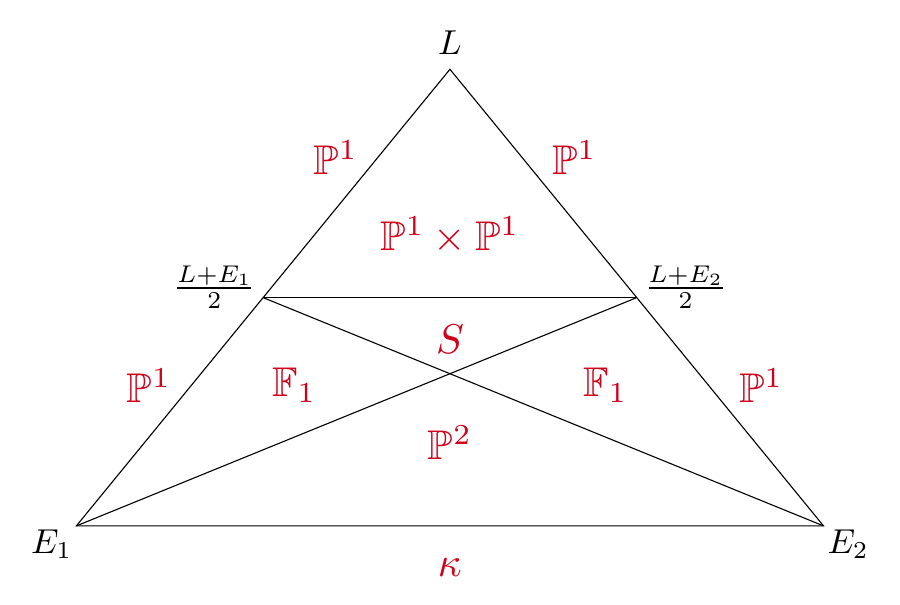
\begin{tikzpicture}[x=0.75pt,y=0.75pt,yscale=-1,xscale=1]
		
		%Shape: Triangle [id:dp7805322996155986] 
		\draw   (300,20) -- (480,240) -- (120,240) -- cycle;
		%Straight Lines [id:da6385330333329691] 
		\draw    (210,130) -- (390,130) ;
		%Straight Lines [id:da012291614577248033] 
		\draw    (210,130) -- (480,240) ;
		%Straight Lines [id:da6507742575307656] 
		\draw    (390,130) -- (120,240) ;
		
		% Text Node
		\draw (210,125) node [anchor=east][inner sep=2pt]  [xscale=1.25,yscale=1.25]  {$\frac{L+E_{1}}{2}$};
		% Text Node
		\draw (390,125) node [anchor=west][inner sep=2pt]  [xscale=1.25,yscale=1.25]   {$\frac{L+E_{2}}{2}$};
		% Text Node
		\draw (120,240) node [anchor=north east][inner sep=1pt]  [xscale=1.25,yscale=1.25]    {$E_{1}$};
		% Text Node
		\draw (480,240) node [anchor=north west][inner sep=1pt]  [xscale=1.25,yscale=1.25]    {$E_{2}$};
		% Text Node
		\draw (300,15) node [anchor=south][inner sep=1pt]  [xscale=1.25,yscale=1.25]   {$L$};
		% Text Node
		\draw (260,75) node [anchor=south east][inner sep=2pt]  [color={rgb, 255:red, 208; green, 2; blue, 27 }  ,opacity=1 ,xscale=1.5,yscale=1.5]  {$\mathbb{P}^{1}$};
		% Text Node
		\draw (170,185) node [anchor=south east][inner sep=2pt]  [color={rgb, 255:red, 208; green, 2; blue, 27 }  ,opacity=1 ,xscale=1.5,yscale=1.5]  {$\mathbb{P}^{1}$};
		% Text Node
		\draw (345,75) node [anchor=south west][inner sep=2pt]  [color={rgb, 255:red, 208; green, 2; blue, 27 }  ,opacity=1 ,xscale=1.5,yscale=1.5]  {$\mathbb{P}^{1}$};
		% Text Node
		\draw (435,185) node [anchor=south west][inner sep=2pt]  [color={rgb, 255:red, 208; green, 2; blue, 27 }  ,opacity=1 ,xscale=1.5,yscale=1.5]  {$\mathbb{P}^{1}$};
		% Text Node
		\draw (300,100) node [anchor=center][inner sep=1pt]  [color={rgb, 255:red, 208; green, 2; blue, 27 }  ,opacity=1 ,xscale=1.5,yscale=1.5]  {$\mathbb{P}^{1}\times\mathbb{P}^{1}$};
		% Text Node
		\draw (240,185) node [anchor=south east][inner sep=2pt]  [color={rgb, 255:red, 208; green, 2; blue, 27 }  ,opacity=1 ,xscale=1.5,yscale=1.5]  {$\mathbb{F}_{1}$};
		% Text Node
		\draw (360,185) node [anchor=south west][inner sep=2pt]  [color={rgb, 255:red, 208; green, 2; blue, 27 }  ,opacity=1 ,xscale=1.5,yscale=1.5]  {$\mathbb{F}_{1}$};
		% Text Node
		\draw (300,260) node [anchor=center][inner sep=0pt] [color={rgb, 255:red, 208; green, 2; blue, 27 }  ,opacity=1 ,xscale=1.5,yscale=1.5]  {$\kappa$};
		% Text Node
		\draw (300,200) node [anchor=center][inner sep=0pt]  [color={rgb, 255:red, 208; green, 2; blue, 27 }  ,opacity=1 ,xscale=1.5,yscale=1.5]  {$\mathbb{P}^{2}$};
		% Text Node
		\draw (300,150) node [anchor=center][inner sep=0pt]  [color={rgb, 255:red, 208; green, 2; blue, 27 }  ,opacity=1 ,xscale=1.5,yscale=1.5]  {$S$};
		
		\end{tikzpicture}
	\end{center}
	
	The decomposition of $T$ describes the geometry of the Mori fibre spaces.
	\begin{enumerate}
		\item Triangles inside $T$ with a side along the boundary correspond to Mori fibre spaces
		\item Shared sides of interior triangles correspond to blowups
		\item All the morphisms (blowups and Mori fibrations) are induced by Abundance for pairs on the corresponding polygon
	\end{enumerate}

	The Sarkisov links between the various Mori fibrations can be seen in the decomposition by composing the birational transformations coming from interior lines meeting at an exterior vertex.

	The ample divisor $A\sim -K_{X}$ plays an important role here. Indeed the key result needed to recreate this kind of decomposition is the following Finiteness of Minimal Models result.
	
	\begin{theo}\label{Main_Finite2}
		Let $R$ be an excellent ring of finite Krull dimension, equipped with a dualising complex and whose residue fields of closed points have characteristic $p>5$ and take $X$ a threefold over $R$. Let $A$ be a big and nef $\mathbb{Q}$-Cartier divisor and $C$ be a rational polytope inside $\mathcal{L}_{A}(V)$. Suppose there is a boundary $A+B \in \mathcal{L}_{A}(V)$ such that $(X,A+B)$ is a klt pair. Then the following hold:
		
		\begin{enumerate}
			\item There are finitely many birational contractions $\phi_{i}:X \dashrightarrow Y_{i}$ such that 
			\[\mathcal{E}(C) = \bigcup \mathcal{W}_{i}=\mathcal{W}_{\phi_{i}}(C)\]
			where each $\mathcal{W}_{i}$ is a rational polytope. Moreover if $\phi:X \to Y$ is a wlc model for any choice of $\Delta \in \mathcal{E}(C)$ then $\phi=\phi_{i}$ for some $i$, up to composition with an isomorphism.
			
			\item There are finitely many rational maps $\psi_{j}:X \dashrightarrow Z_{j}$ which partition $\mathcal{E}(C)$ into subsets $\mathcal{A}_{\psi_{j}}(C)=\mathcal{A}_{i}$.
			\item  For each $W_{i}$ there is a $j$ such that we can find a morphism $f_{i,j}: Y_{i} \to Z_{j}$ and $W_{i} \subseteq \overline{A_{j}}$.
			\item  $\mathcal{E}(C)$ is a rational polytope and $A_{j}$ is a union of the interiors of finitely many rational polytopes.
		\end{enumerate}
	\end{theo}
	
	The keys ideas of the proof come from \cite{BCHM10}. The main difficulty in mixed characteristic is the lack of appropriate Bertini type theorems. There are sufficient results to prove the result over local rings, with some modifications to the original proof. Some work is needed, however, to translate a local version of the result to a more general one. 
	
	Though it does seem it should be possible, we take a slightly different approach. First introducing a notion of an rlt pair, one which is replaceable by a klt pair locally over the base. This allows us to essentially extend the local Bertini result to a global one, at the cost of a slightly more complicated type of pair. With this accounting system in place, the finiteness result is essentially no harder to prove over an arbitrary base than over a local ring. The proofs given rely only on the MMP, and will generalise immediately to higher dimensions if the appropriate MMP results are known. 
	
	These rlt pairs are also useful for working with Sarkisov links. Once again there are not sufficiently strong Bertini type results to produce a klt pair corresponding to the flops of a Sarkisov link, instead an rlt pair is needed.
	
	In this Chapter we also give a short proof of termination for klt threefold pairs in mixed characteristic; showing that any MMP from a pair with $K_{X}+\Delta$ not psuedo-effective eventually terminates with a Mori Fibration.
	
	\begin{theo}\label{Main_Finite3}[\autoref{termination}]
		Let $R$ be an excellent ring of finite Krull dimension, equipped with a dualising complex and whose residue fields of closed points have characteristic $p>5$.
		Let $f:(X,\Delta) \to T$ be a threefold klt pair over $R$, then any $K_{X}+\Delta$ MMP terminates.
	\end{theo}
	
	\section{The Augmented Base Locus}
	
	In addition to the earlier results related to the MMP and its applications we also study some more technical birational geometry results. The focus is largely on nef line bundle on mixed characteristic schemes which are semiample in characteristic $0$.
	
	The augmented base locus is well studied for schemes over a field. It is defined as follows.
	
	\begin{definition}
		Let $L$ be a line bundle on a projective Noetherian scheme $X$. Then base locus is given as 
		$$\BB(L)= \bigcap_{s \in H^{0}(X,L)} Z(s)_{red}$$
		where $Z(s)$ is the zero set of $s$ equipped with the obvious scheme structure. The stable base locus is then
		$$\SB(L)=\bigcap_{m \geq 0}\BB(mL).$$
		Fix an ample line bundle $A$. The augmented base locus is given as 
		$$\BS(L)=\bigcap_{m \geq 0}\SB(mL-A)$$
		and is independent of the choice of $A$.
		
	\end{definition} 
	
	An important characterisation of the augmented base locus, first noted for smooth varieties of characteristic $0$ by Nakayame \cite{nakamaye2000stable}, is that for a nef line bundle $L$ the augmented base locus $\BS(L)$ agrees with the exceptional locus $\mathbb{E}(L)$. 
	
	Since then the result has been shown to hold for projective schemes over a field, first in positive characteristic by Cascini-M\textsuperscript{c}Kernan-Musta\c{t}\v{a} \cite{cascini2014augmented}, and then for $\mathbb{R}$-divisors over any field by Birkar \cite{birkar2017augmented}. Similar results are given for non-nef divisors in \cite{ein2009restricted} and for K\"{a}hler manifolds in \cite{collins2015kahler}.
	
	We make use of methods developed in \cite{witaszek2020keel} together with ideas from the positive characteristic proof to show that $\BS(L)=\mathbb{E}(L)$ for a nef line bundle on a projective scheme over an excellent Noetherian base, so long it holds true on the characteristic zero part the scheme. In particular the result holds in the following cases.
	
	\begin{theorem}[\autoref{Main_Loci}]
		Let $X$ be a projective scheme over an excellent Noetherian base $S$ with $L$ a nef line bundle on $X$. 
		Suppose that one of the following holds:
		\begin{enumerate}
			\item $S_{\mathbb{Q}}$ has dimension $0$;
			\item $L|_{X_{\mathbb{Q}}}$ is semiample;
		\end{enumerate}
		
		Then $\BS(L)=\mathbb{E}(L)$.
	\end{theorem}
	
	We also extend the semiampleness result of \cite{witaszek2020keel} to show that there is an equality of stable base loci when the characteristic $0$ part is semiample.
	
	\begin{theorem}[\autoref{Main_Loci2}]
		Suppose that $X$ is a projective scheme over an excellent Noetherian base with $L$ a nef line bundle on $X$. Then $\SB(L)=\SB(L|_{\mathbb{E}(L)})$ so long as $L|_{X_{\mathbb{Q}}}$ is semiample.
	\end{theorem} 
	
	
	
	
	
	%\documentclass[a4paper,12pt]{book}
\usepackage[a4paper, margin=1in]{geometry}
\setlength{\parindent}{0cm}
\setlength{\parskip}{1\baselineskip}

\setcounter{secnumdepth}{4}
\usepackage{amsthm}
\usepackage{aliascnt}
\usepackage{amsmath,amssymb,amsfonts}
\usepackage{hyperref}
\usepackage[shortlabels]{enumitem}

\usepackage{tikz-cd}

\newcommand{\basetheorem}[3]{
	\newtheorem{#1}{#2}[#3]
	\newtheorem*{#1*}{#2}
	\expandafter\def\csname #1autorefname\endcsname{#2}
}
\newcommand{\maketheorem}[3]{
	\newaliascnt{#1}{#3}
	\newtheorem{#1}[#1]{#2}
	\aliascntresetthe{#1}
	\expandafter\def\csname #1autorefname\endcsname{#2}
	\newtheorem{#1*}{#2}
}

%\theoremstyle{plain}
\basetheorem{theorem}{Theorem}{section}
\maketheorem{definition}{Definition}{theorem}
\maketheorem{lemma}{Lemma}{theorem}
\maketheorem{example}{Example}{theorem}
\maketheorem{corollary}{Corollary}{theorem}
\maketheorem{conjecture}{Conjecture}{theorem}
\maketheorem{proposition}{Proposition}{theorem}
\maketheorem{question}{Question}{theorem}
\maketheorem{remark}{Remark}{theorem}

\makeatletter
\newcommand{\newreptheorem}[2]{\newtheorem*{rep@#1}{\rep@title}\newenvironment{rep#1}[1]{\def\rep@title{#2 \ref*{##1}}\begin{rep@#1}}{\end{rep@#1}}}
\makeatother
\makeatletter
\@namedef{subjclassname@2020}{%
	\textup{2020} Mathematics Subject Classification}
\makeatother


%\newreptheorem{theorem}{Theorem}

%begin: Iacopo-defined newcommands
\DeclareMathOperator{\Spec}{Spec}
\DeclareMathOperator{\Proj}{Proj}
\newcommand{\bP}{\mathbb{P}}
\newcommand{\bR}{\mathbb{R}}
\newcommand{\bQ}{\mathbb{Q}}
\newcommand{\bN}{\mathbb{N}}
\newcommand{\bZ}{\mathbb{Z}}
\newcommand{\fB}{\mathbf{B}}
\newcommand{\fM}{\mathbf{M}}
\newcommand{\charac}{\textup{char }}
\newcommand{\id}{\textup{id}}
\newcommand{\Alb}{\textup{Alb}}
\newcommand{\cO}{\mathcal{O}}
\newcommand{\red}{\textup{red}}
\newcommand{\lct}{\textup{lct}}
\newcommand{\exc}{\textup{Ex}}
\newcommand{\coeff}{\textup{coeff}}
\newcommand{\cent}{\textup{centre}}
\newcommand{\codim}{\textup{codim}}
\newcommand{\textoverline}[1]{$\overline{\mbox{#1}}$}
\newcommand{\rk}{\textup{rk}}
\newcommand{\WDiv}{\textup{WDiv}}
%end: Iacopo-defined newcommands


\newcommand{\A}{\mathcal{A}}
\newcommand{\B}{\mathcal{B}}
\newcommand{\C}{\mathcal{C}}
\newcommand{\D}{\Delta}
\newcommand{\Vol}{\text{Vol}}
\newcommand{\Sing}{\text{Sing}}
\newcommand{\E}{\mathcal{E}}
\newcommand{\F}{\mathcal{F}}
\newcommand{\PP}{\mathcal{P}}
\newcommand{\HH}{\mathcal{H}}
\newcommand{\SB}{\mathbf{SB}}
\newcommand{\BS}{\mathbf{B}_{+}}
\newcommand{\disc}{\text{Discrepancy}}


\newcommand{\ta}[1]{\mathcal{A}^{\leq #1}}
\newcommand{\at}[1]{\mathcal{A}^{\geq #1}}
\newcommand{\tb}[1]{\mathcal{B}^{\leq #1}}
\newcommand{\bt}[1]{\mathcal{B}^{\geq #1}}
\newcommand{\tc}[1]{\mathcal{C}^{\leq #1}}
\newcommand{\ct}[1]{\mathcal{C}^{\geq #1}}
\newcommand{\nklt}{\text{Nklt}}
\newcommand{\Ht}[1]{H^{i}_{t}}
\newcommand{\orth}{^{\perp}}
\newcommand{\Hom}{\text{Hom}}
\newcommand{\Fe}{F^{e}_{*}}
\newcommand{\Fn}[1]{F^{#1}_{*}}
\newcommand{\trip}{(R,\Delta, \alpha_{\bullet})}
\newcommand{\ai}{\alpha_{\bullet}}
\newcommand{\im}{\text{Im}}
\newcommand{\ox}{\mathcal{O}_{X}}
\newcommand{\me}{M^{e}_{\Delta,a^{t}}}
\newcommand{\psim}{\sim_{\mathbb{Z}_{(p)}}}
\newcommand{\zp}{\mathbb{Z}_{(p)}}
\newcommand{\Xde}[1]{\mathcal{X}_{\delta,\epsilon,#1}}
\newcommand\myworries[1]{\textcolor{red}{#1}}

\begin{document}
\chapter{Preliminaries}
\section{Singularity Theory}

We begin by collecting relevant notions of singularities for the minimal model program in mixed and positive characteristic. These include classic notions coming from the characteristic $0$ setting, as well as algebraic singularity conditions developed in the positive characteristic setting.

\subsection{Singularities of pairs}
Here $\mathbb{K}$ will be taken to mean either $\mathbb{R}$ or $\mathbb{Q}$. If no field is specified, it is taken to be $\mathbb{R}$.

In full generality we have the following set-up.

\begin{definition}\label{setup}
	An $R$-pair $(X,\Delta)/ T$ with $\mathbb{K}$-boundary will be the following data:
	\begin{itemize}
		\item An excellent, normal ring $R$ of finite dimension which admits a dualising complex and whose residue fields have characteristic at least $5$;
		\item A quasi-projective $R$-variety $T$;
		\item A normal, integral scheme $X$ projective over $T$; and
		\item A $\mathbb{K}$-divisor $\Delta \geq 0$ with $(K_{X}+\Delta)$ $\mathbb{K}$-Cartier, for $\mathbb{K}=\mathbb{R}$ or $\mathbb{Q}$.
	\end{itemize}
	
	The dimension of such a pair is the dimension of $X$. Equally the pair is said to $\mathbb{Q}$-factorial if $X$ is.
\end{definition}

\begin{remark}
	
	We require the relative data of $R$ and $T$ so that the notion of an $R$-pair captures the the kind of MMPs we wish to run. Many notions of singularity do not depend on this data however, instead many of them are local on $X$. For such notions we may work affine locally on $X$ and let $X \to T \to R$ be the identity map to recover these as intrinsic notions of singularity.
\end{remark}

In practice we will often have $T=R$. In this case we omit $T$ from the notation and say only that $(X,\Delta)$ is an $R$-pair. If further $R=\kappa$ is a field, we often say one that $(X,\Delta)$ is a pair over a field or just that $(X,\Delta)$ is a pair, depending on context.

We will often ask that $X \to T$ has positive dimensional image, in this case we just say $(X,\Delta)/T$ is an $R$-pair with positive dimensional image. This is because many results for threefolds are not known in greater generality than this, for example much is unknown when $X$ is a variety over a perfect field.

In cases where $R$ is clear from context we often describe an $R$-pair with $\mathbb{K}$-boundary as a $\mathbb{K}$-pair. While we will sometimes work with schemes over a field of characteristic $0$, it will never be relevant whether that field is $\mathbb{Q}$ or $\mathbb{R}$. Therefore a $\mathbb{K}$-pair will only ever mean a pair with coefficients in $\mathbb{K}$ and never pair whose underlying scheme is of finite type over the field $\mathbb{K}$. 

\begin{definition}
	If $\Delta$ is not effective but $(X,\Delta)/T$ would otherwise be an $R$-pair with $\mathbb{K}$ boundary we call it an $R$-sub-pair with $\mathbb{K}$ boundary.
	
	The index of a (sub)-pair (resp. $\mathbb{Q}$ Gorenstein variety) is the minimal $r>0$ with $r(K_{X}+\Delta)$ ($rK_{X}$) Cartier.
\end{definition}

Suppose that $X$ is $\mathbb{Q}$-Gorenstein with index $m$. Let $Y$ be an integral, normal scheme then given a projective birational morphism $f:Y \to X$ we have a canonical identification $f^{*}mK_{X}+\sum(ma_{i})E_{i}=mK_{Y}$, where $E_{i}$ are exceptional. For simplicity we write $f^{*}K_{X}+\sum a_{i}E_{i} =K_{Y}$.

More generally if $(X,\Delta)$ is an $R$-sub-pair of index $r$ we may write $f^{*}(K_{X}+\Delta)=K_{Y}+ \Delta_{Y}$ where $\Delta_{Y}=\sum -a(Y,E,X,\Delta)E$ agrees with $\Delta$ away from the exceptional locus. Then $(Y,\Delta_{Y})$ is a sub pair of index $r_{Y}$ dividing $r$. Clearly pulling back $k(K_{X}+\Delta)$ where $r|k$ does not change the outcome.

Suppose that there are normal, integral schemes $Y_{i}$ with $f_{i}:Y_{i} \to X$ birational and there is a some normal, integral scheme $Z$ with $g_{i}:Z\to Y_{i}$. If $E_{i}$ are divisors on $Y_{i}$ with a common strict transform $E$ then $a(Z,E,X,\Delta)=a(Z,E,Y_{i},\Delta_{Y_{i}})=a(Y_{i},E_{i},X,\Delta)$ since we have $g_{i}^{*}f_{i}^{*}r(K_{X}+\Delta)=g_{i}^{*}r(K_{Y_{i}}+\Delta_{Y_{i}})$.

We may view then divisors on $a(Y,E,X,\Delta)$ as being independent of the model $Y$ and write $a(E,X,\Delta)$ instead. 

For every prime divisor $E$ on a birational model, $Y$, of $X$ we have an associated DVR $\mathcal{O}_{Y,E}$, the stalk at the generic point of $E$ which gives a valuation, $\nu_{E}$ on the function field $K(X)$. If $f:Y \to X$ is a birational morphism and $D$ a Cartier divisor on $D$ together with a choice of generator inside $K(X)$ then pulling back $D$ and looking at its coefficient at $E$ is equivalent to asking for the valuation under $\nu_{E}$. 

In general, the converse is false. Not every valuation can be applied to $K_{X}$ in this fashion.

For example suppose $X$ is a proper normal variety over a field which is not $\mathbb{Q}$-Gorenstein. Let $U$ be the smooth locus and $P$ at which $X$ is not $\mathbb{Q}$-Gorenstein. We may blowup $X$ at $P$ to give $Y \to X$ with $E$ lying over $P$. Then $U$ is smooth and birational to $Y$, but we cannot take the valuation of $K_{U}$ with respect to $E$ since no multiple of $K_{U}$ is Cartier on $X$. If we wish to think of the $a(X,\Delta,E)$ as coming from valuations we must, therefore, consider only those with non-empty center on $X$. 

\begin{definition}
	Let $A$ be an integral domain with $\text{Frac}(A)=K$ and $R$ a DVR in $K$ with maximal ideal $m_{R}$. Then the center of $R$ in $A$ is $m_{R}\cap A$. We extend the definition to normal, integral schemes in the natural fashion.
\end{definition}

If $X$ is of finite type over a locally Noetherian scheme $T$ then $X$ is proper over $T$ if and only if every $T$-valuation has non-empty centre on $X$, by the valuative criterion of properness \cite{stacks-project}[Tag 0208]. 

Equally for a prime divisor $E$ on a birational model $Y$ of $X$, we can think of it as having non-empty centre on $X$ if there is a dominating model $Z \to X,Y$ such that the generic point of $E$ is contained in the image of $Z$ on $Y$. This is the same as asking for the valuation it induces to have non-empty centre on $X$. In fact we can realise the centre of the valuation is the closure of the strict transform of $E$.

For simplicity, we will always think of a divisor $E$ with non-empty centre on $X$ as lying on a model $Y$ which dominates $X$. Since the valuation does not depend on the birational model, we can always choose a higher model to ensure this is a valid assumption. 

\begin{definition}
	
	Let $\pi:Y \to X$ be a proper birational morphism of integral, normal $R$ schemes. A divisor $E$ on $Y$ is said to be exceptional if $\pi$ is not an isomorphism at the generic point of $E$, or equally if the centre of $E$ is not a divisor on $X$.
	
	Given a sub-pair $(X,\Delta)$ we define the discrepancy $$\text{Disc}(X,\Delta):=\inf \{a(E,X,\Delta) \text{ such that } E \text{ is exceptional and has non-empty center on } X\}$$
	and the total discrepancy 
	
	$$\text{TDisc}(X,\Delta):=\inf \{a(E,X,\Delta) \text {such that } E \text{ has non-empty center on } X\}$$
\end{definition}

We then use this define a suite of singularities.

\begin{definition}
	Let $(X,\Delta)/T$ be an $R$-(sub)-pair then we say that $(X,\Delta)/T$ is
	\begin{itemize}
	\item 	(sub) terminal if $\text{Disc}(X,\Delta) > 0$
	\item	(sub) canonical if $\text{Disc}(X,\Delta)\geq 0$
	\item 	(sub) plt if $\text{Disc}(X,\Delta)\geq -1$
	\item	(sub) $\epsilon$-klt if $\text{TDisc}(X,\Delta) > \epsilon-1$
	\item	(sub) $\epsilon$-lc if $\text{TDisc}(X,\Delta) \geq \epsilon -1$
	\end{itemize}
\end{definition}

\begin{remark}
	
	Klt is short for Kawamata log terminal and lc is short for log canonical.
	\end{remark}

For $\epsilon=0$ we say klt, lc respectively. An equivalent formulation of lc is that $\text{Disc}(X,\Delta) \geq -1$ as this condition ensures that $\Delta$ has coefficients bounded above by $1$.

\begin{lemma}
	
	Let $(X,\Delta)/T$ be an $R$-(sub)-pair with $\text{Disc}(X,\Delta) \geq -1$, then $X$ is lc.
	
	\end{lemma}

\begin{proof}
Since $X$ is normal we may pick $D$ in the support $\Delta$ and localise at $Q$ a point of codimension $2$ inside the smooth locus of $X$ and $D$ which meets no other component of $\Delta$. This reduces us to the case that $X$ is smooth of dimension $2$ and the support of $D$ is a smooth curve, $C$. Now suppose for contradiction that $D=(1+\epsilon)C$ for $\epsilon > 0$. If we blow up the closed point, we get an exceptional divisor $E$ with $a(E,X,\Delta)=-\epsilon$. Blowing up the intersection of $E$ and the strict transform of $\Delta$ gives $E_{2}$ with $a(E_{2},X,\Delta)=-2\epsilon$. Continuing in this fashion we can find $E_{n}$ with $a(E_{n},X,\Delta)=-n\epsilon< -1$ for some suitably large $n$.

Since $\text{Disc}(X,\Delta) \geq -1$ no such $E_{n}$ can exist, so the result holds by contradiction.
\end{proof}

Note that if $\Delta \geq B$, clearly $a(E,X,\Delta) \leq a(E,X,B)$ so $(X,B)$ cannot have singularities which are worse, in the above sense, than $(X,\Delta)$. Moreover if $(X,\Delta)$ is sub $\epsilon$-lc and $(X,B)$ is sub $\epsilon$-klt then so is any sub-pair  $(X,D)$ with $D \leq \delta B+(1-\delta)\Delta$ for any $1>\delta >0$.

When we have resolution of singularities there is another, more practical version of these definitions.

\begin{definition}
	
	We say $(X,\Delta)/T$ is log smooth (resp. regular) if $X$ is a smooth (resp. regular) $T$-scheme and $\Delta=\sum d_{i}D_{i}$ is a divisor with normal crossing support
	
	If $(X,\Delta)/T$ is an $R$ pair and $\pi:Y \to X$ is projective, birational morphism with exceptional locus $E$ such that $(Y,\pi^{-1}_{*}\Delta+E)$ is log regular then $\pi:Y\to X$ is a log resolution of $(X,\Delta)$. In this case, we sometimes say $\pi:Y \to (X,\Delta)$ is a log resolution.
	
\end{definition}

\begin{remark}
	
	In principle it is enough for a log resolution to be proper for the purposes of these valuative notions of singularity. In practice we will often want projective log resolutions for other reasons and we do not separate the notions.
	
	\end{remark}

\begin{lemma}
	Suppose that $(X,\Delta)/T$ is log regular. Let $E$ be a prime divisor with center $V\neq E$ on $X$, write $P$ for the generic point of $V$. 
	Then \begin{enumerate}
		\item $a(E,X,D)\geq codim(P,X) -1-\sum_{i: P\in D_{i}}d_{j}$
		\item $\text{TDisc}(X,\Delta)=\min\{0,-d_{i}\}$
		\item $\text{Disc}(X,\Delta) =\min\{1,1-d_{i},1-d_{i}-d_{j}\text{: } D_{i} \cap D_{j}\neq \emptyset\}$

	\end{enumerate}
\end{lemma}
\begin{proof}
	Let $Y \to X$ be a birational morphism such that $E$ is a divisor on $Y$, let $Q$ be its generic point. Localise at $P$ in $X$ so we may suppose that $P$ is closed and given by the vanishing of $x_{1},...x_{n}$ where $n=\text{codim}(P,X)$. Similarly we may suppose $E$ is given as the vanishing of a local coordinate $y_{1}$ on $Y$. Since $(X,\Delta)$ is log regular we may, after reordering, suppose $D_{1},..D_{k}$ contain $P$ and each is given as the vanishing of a local coordinate $x_{i}$. Further can write $f^{*}x_{i}=y_{1}^{a_{i}}u_{i}$ where $u_{i}$ does not vanish at $Q$ and $a_{i}\in \mathbb{Z}_{>0}$ .
	
	We then have $$f^{*}dx_{i}=a_{i}y_{i}^{a_{i}-1}u_{i}dy_{1} + y_{1}^{a_{i}}du_{i}$$ by the chain rule where $du_{i}=w_{i}$ are regular at $Q$.
	
	Putting $c_{i}=d_{i}$ for $i \leq k$ and $c_{i}=0$ otherwise gives
	$$f^{*}\frac{dx_{i}}{x_{i}^{d_{i}}}=a_{i}y_{1}^{(1-c_{i})a_{i}-1}u_{i}^{1-c_{i}}dy_{1} +y_{1}^{(1-c_{i})a_{i}}w_{i}.$$
	
	However then we see that the only possible poles of 
	$$f^{*}\frac{dx_{1}\wedge...\wedge dx_{n}}{x_{1}^{c_{1}}...x_{n}c^{n}}$$
	at $Q$ come from 
	
	$$y_{1}^{A_{i}}dy_{1}\wedge w_{1}\wedge ... \wedge w_{i-1} \wedge w_{i+1} \wedge... \wedge w_{n}$$
	with $$A_{i}=-1+ \sum_{1}^{n} (1-c_{j})a_{j} \geq -1+\sum _{1}^{n}a_{j} -\sum_{1}^{k} d_{j}a_{j} \geq n -1 - \sum_{1}^{k} d_{j},$$ giving $(1)$.
	
	For any $E$ with center $V$ we have $a(E,x,D) \geq \text{codim}(V,X) -1 - \sum_{V \subseteq D_{i}} d_{i}$ and since $d_{i} \leq 1$ for every $i$ the smallest value occurs when $V=E$ has codimension $1$ and we obtain $\text{TDisc}(X,\Delta)=\min\{0,-d_{i}\}$. Similarly if $E$ is required to be exceptional we must have the smallest values when $V$ has dimension $2$ so that $\text{Disc}(X,D)\geq \min\{1,1-d_{i},1-d_{i}-d_{j} \text{ such that }D_{i}\cap D_{j} \neq \emptyset\}$.
	
	 Suppose however we blow up $V\subseteq D_{i}$ of codimension $2$ and label the exceptional divisor $E$. It is an easy calculation that $a(E,X,D)=1-d_{i}$ if $V\not\subseteq D_{j}$ for all $j$ else $a(E,X,D)=1-d_{i}-d_{j}$ where $V \subseteq D_{j}$ giving $2$. Similarly by blowing up $V$ of codimension $2$ not contained in any $D_{i}$ we see that there is some $E$ with $a(X,E,D)=1$ so $(3)$ holds.
	 
\end{proof}


 Indeed as $X$ is normal, we may restrict to an open set and assume that $\Delta$ is a prime divisor with $(X,\Delta)$ log smooth. Now blowing up along $V$ inside $\Delta$ of codimension $2$, we may instead assume that 

\begin{corollary}
	Let $(X,\Delta)/T$ be an $R$-(sub)-pair and $\pi:Y\to X$ a log resolution of $(X,\Delta)$. Let $$t=\min\{a(E,X,\Delta) \text{ such that } E \text{ is a divisor on } Y\}$$ and $$d=\min\{a(E,X,\Delta) \text{ such that } E \text{ is an exceptional divisor of } \pi:Y\to X\}.$$
	Then
		\begin{itemize}
		\item 	(sub) terminal if $d > 0$
		\item	(sub) canonical if $d\geq 0$
		\item 	(sub) plt if $d > -1$
		\item	(sub) $\epsilon-klt$ if $t > \epsilon-1$
		\item	(sub) $\epsilon-lc$ if $t\geq \epsilon -1$
	\end{itemize}
\end{corollary}

This also gives rise to an additional notion of singularity.

\begin{definition}
	An $R$ pair $(X,\Delta)/T$ is called dlt if it lc and there is a closed subscheme $Z \subseteq Z$ such that:
	
	\begin{itemize}
		\item $X\setminus Z$ is smooth, 
		\item $\Delta|_{X\setminus Z}$ is simple normal crossing
		\item If $E$ is an exceptional divisor with centre in $Z$ then $a(E,X,\Delta) > -1$.
	\end{itemize}
	
	
	 
\end{definition}

Roughly speaking this says a dlt pair is a lc pair with is klt away from the locus where it is log smooth.

Note that if $(X,\Delta)$ is plt then it is also dlt, moreover $\lfloor \Delta \rfloor$ must have disjoint support.

\begin{remark}
	
	We can also characterise dlt with reference to a log resolution as follows. A pair $(X,\Delta)/T$ is dlt if there is a log resolution $\pi:Y \to X$ of $(X,\Delta)$ with $K_{Y}+\Delta_{Y}=\pi^{*}(K_{X}+\Delta)$ such that $\text{Coeff}_{E}(\Delta_{Y}) < 1$ for every $E$ exceptional.
	
	This definition is not independent of the resolution. Consider for example $X$ a smooth surface with $\Delta=C_{1}+C_{2}$ with connected log smooth support. This is trivially dlt, however if we blow up a point $P$ in $C_{1}\cap C_{2}$ then the pullback of $K_{X}+\Delta$ has coefficient $1$ at the exceptional divisor.

\end{remark}

Allowing sub-pairs, being klt, lc etc pulls back naturally along birational morphisms. The following lemma allows us to push forward along them as well.

\begin{lemma}[Negativity Lemma]
	Let $f:X \to Y$ be a projective birational morphism of normal varieties. Let $D$ be an $\mathbb{R}$ Cartier divisor on $X$ with $-D$ nef over $Y$. Then $D$ is effective if and only if $f_{*}D$ is.
\end{lemma}

%\begin{lemma}
%	Suppose that $(X,\Delta)$ is a pair equipped with a morphism $f:X \to Y$. Suppose that $(Y,f_{*}\Delta)$ is a pair, that is $K_{Y}+f_{*}\Delta$ is $\mathbb{R}$-Cartier, and that $-(K_{X}+\Delta)$ is nef over $Y$. Then given $Z\to X$ a birational morphism of normal varieties, and $E$ a divisor on $Z$, we have $a(E,X,\Delta) \leq a(E,Y,f_{*}\Delta)$
%\end{lemma}
%\begin{proof}
%	Consider 
%	\[D=f^{*}(K_{Y}+f_{*}\Delta)-(K_{X}+\Delta)\]
%	which is nef over $Y$ by assumption. Then $-f_{*}D=0$, and in particular is effective, giving that $-D$ is effective by the negativity lemma. Hence we have $(K_{X}+\Delta) \geq  f^{*}(K_{Y}+f_{*}\Delta)=(K_{X}+\Delta')$, and so $a(E,Y,f_{*}\Delta)=a(E,X,\Delta') \geq a(E,X,\Delta)$ as required. 
%\end{proof}
%
%More generally we have the following.

\begin{lemma}
	Suppose $(X,\Delta)/T,(X',\Delta')/T$ are $R$-pairs equipped with projective birational $T$-morphisms $f:X \to Y$ and $f':X'\to Y$ with $f_{*}\Delta=f'_{*}\Delta'$.
	
	Suppose further that $-(K_{X}+\Delta)$ is $f$ nef and $(K_{X'}+\Delta')$ is $f'$ nef. Then $a(E,X,\Delta) \leq a(E,X',\Delta')$ for any $E$ with non-trivial center on $Y$.
\end{lemma}
\begin{proof}
	Let $Z$ be a normal scheme with projective, birational morphisms $g:Z \to X$ and $g':Z \to X'$, write $h=f \circ g=f' \circ g'$. Let $D= g^{*}(K_{X}+\Delta)-g'^{*}(K_{X'}+\Delta')$ which is exceptional by construction. Further since nefness is preserved under pulllback, $-H$ is nef over $Y$ and hence we may apply the negativity lemma to see that $H$ is effective. Hence $g^{*}(K_{X}+\Delta) \leq g'^{*}(K_{X'}+\Delta')$. In particular if $E$ is any divisor on $Z$, then $a(E,X,\Delta) \leq a(E,X,\Delta')$.
	
	Suppose now $E$ is a valuation with non-trivial center on $Y$. There is some $Z \to Y$ with $E$ a divisor on $Z$. We may then resolve the indeterminacy of $Z \to X$ and $Z \to X'$ and assume wlog that $Z$ lies over $X,X'$ also and the result follows.
\end{proof}

This is exactly the result that shows these notions of singularity are preserved under a $(K_{X}+\Delta)$ MMP.

\myworries{State and prove}

%\begin{definition}
%	A (sub) $\epsilon$-lc pair $(X,\Delta)/T$ where $K_{X}+\Delta \equiv_{T} 0$ is said to be (Sub) $\epsilon$-log Calabi-Yau, or just (sub) $\epsilon$-LCY. 
%\end{definition}
%Again for $\epsilon=0$ we just say LCY.
%\begin{corollary}
%	Suppose that $(X,\Delta)$ is $\epsilon$-LCY and $f:X\dashrightarrow X'$ is either a flip or a divisorial contraction then $(X',f_{*}\Delta)$ is $\epsilon$-klt.
%\end{corollary}
%\begin{proof}
%	Both $(K_{X}+\Delta)$ and $(K_{X'}+\Delta')$ are numerically trivial so it suffices to show that $(K_{X'}+\Delta')$ is $\mathbb{R}$ Cartier. 
%	
%	Note then that if $g:X \to Y$ is the contraction of an extremal ray and $D\equiv_{g} 0$ is Cartier, there is some $L$ Cartier on $Y$ with $g^{*}L=D$. If $f$ is a divisorial contraction then $r(K_{X}+\Delta)=f^{*}L$ say and so $r(K_{X'}+\Delta')=L$ by the projection formula. Else $f$ is a flip and there is $g:X \to Y$ a flipping contraction together with $g':X' \to Y$ such that $f=g'^{-1}\circ g$. Hence writing $r(K_{X}+\Delta)=g^{*}L$ again gives $r(K_{X'}+\Delta')=g'^{*}L$.
%\end{proof}

\subsection{Frobenius singularities}

This section will focus on Frobenius singularities in positive characteristic. These will only be needed for schemes over a field. We will often work with varieties over a field $\kappa$, which here will mean just mean integral, quasi-projective $\kappa$-schemes.

\subsubsection{Frobenius singularities of pairs}

\begin{definition}
Given a $\kappa$ algebra $R$ over positive characteristic we denote the Frobenius morphism by $F:R\to R$ sending $x \to x^{p}$. Any $R$ module $M$ then has an induced module structure, denoted $F_{*}M$ where $R$ acts as $r.x=F(x)r=r^{p}m$. Finally $R$ is said to be $F$-finite if $F_{*}R$ is a finite $R$ module. This is a particularly important notion in the case that $R=\kappa$.

These definitions naturally extend to schemes over $\kappa$. 
\end{definition}

Note that all perfect fields are $F$-finite. Moreover any finitely generated algebra over an $F$-finite field is itself $F$-finite. In particular varieties over an $F$-finite field are $F$-finite.

In this context we can view the Frobenius morphism as a map of $R$ modules $F:R \to F_{*}R$. We will also write $F^{e}:R \to F_{*}^{e}R$ for the $e^{th}$ iterated Frobenius.

We have the following well known result due to Kunz.

\begin{theorem}
	Let $R$ be a local ring of characteristic $p> 0$, then $R$ is regular if and only if $F_{*}R$ is a flat $R$ module.
\end{theorem}

It is natural then to try and understand the singularities of a scheme via flatness conditions on $F_{*}R$. In the first instance we have the following definitions.

\begin{definition}
	Let $X$ be a normal variety over an $F$-finite field.
	We say $X$ is:
	\begin{itemize}
		\item $F$-pure if the Frobenius morphism $\ox \to F_{*}\ox$ is pure, or equivalently locally split.
		\item (Globally) $F$-split if the Frobenius morphism $\ox \to F_{*}\ox$ is split.
	\end{itemize} 
\end{definition}

Here for a morphism $f:R \to S$ to be pure means the induced map $M \to M \times S$ is injective for every $R$ module $M$. When $S$ is a finite $R$ module, $f$ is pure if and only if it is split. That is there is a morphism $g:S \to R$ of $R$ modules with $g \circ f =id$.

\begin{remark}

	This purity condition is closed related to both flatness and effective descent. Roughly speaking every flat morphism is an effective descent morphism, but in general an effective descent morphism need only be pure. In fact purity turns out to be a sufficient condition also \cite[Tag 08WE]{stacks-project}.
	
	In particular regular varieties are $F$-pure.
	
	\end{remark}

While useful definitions, for the purposes of the MMP we would like ones which can be more naturally applied to pairs $(X,\Delta)$.

Take $X$ a normal variety over an $F$-finite field. To mirror the notion of a boundary we introduce pairs $(\mathcal{L}, \phi)$ where $\mathcal{L}$ is a line bundle and $\phi: \Fe \mathcal{L} \to \ox$. By applying duality on the smooth locus, which contains all the codimension $1$ points, we observe that $\Hom_{\ox}(\Fe \mathcal{L},\ox)=H^{0}(X,\mathcal{L}^{-1}((1-p^{e})K_{X}))$. Therefore such a pair corresponds to a divisor $\Delta_{\phi} \geq 0$ with $(p^{e}-1)(K_{X}+\Delta_{\phi}) \sim \mathcal{L}$. Reversing this procedure is slightly more involved. If ${(p^{e}-1)(K_{X}+\Delta) \sim \mathcal{L}}$ (we sometimes write this $K_{X}+\Delta \sim_{\zp} \mathcal{L}$) we may obtain $\phi_{\Delta}:\Fe \mathcal{L} \to \ox$, however we could also write say $(p^{2e}-1)(K_{X}+\Delta) \sim \mathcal{L'}$ where $\mathcal{L'} \not\sim \mathcal{L}$. We introduce, therefore, the following notion of equivalence.

First, we say that two such pairs, $(\mathcal{L}, \phi)$ and $(\mathcal{L}', \phi')$ are said to be equivalent if

\begin{itemize}
	\item The following diagram is well defined and commutes.
	\[\begin{tikzcd}
	\Fe \mathcal{L} \arrow[rd, "\phi"] \arrow[rr, "\Fe \psi"] &     & \Fe \mathcal{L}' \arrow[ld, "\phi'"] \\
	& \ox &                                     
	\end{tikzcd}\]
	\\
	\item OR $\mathcal{L}=\mathcal{L}^{p^{(n-1)e+...+1}}$ and $\phi':F_{*}^{ne}\mathcal{L}^{p^{(n-1)e+...+1}}$ is the map generated by composing appropriate tensor products of the form $F_{*}^{m}\mathcal{L}^{k} \otimes F_{*}^{n} \mathcal{L}^{r}\cong F_{*}^{m}(\mathcal{L}^{rp^{m-n}+k}) \to F^{m}_{*}\mathcal{L}^{k}\to \ox$ for $m>n$.
\end{itemize}

We then expand the notion of equivalence to allow any finite combination of the above equivalences, more precisely we take the transitive closure of our initial equivalence relation. In fact we will see that any two equivalent pairs are connected by a step of each type.

The need for first part of this is clear. The second comes from the following lemma

\begin{lemma}\label{twist}
	Suppose that $(\mathcal{L},\phi)$ and $(\mathcal{L}',\phi')$ are pairs as above. Then we have the following map
	\[\psi= \phi' \circ_{F} \phi: F^{e+e'}_{*}(\mathcal{L}\otimes (\mathcal{L}')^{p^{e}})\cong F_{*}^{e'}(\Fe \mathcal{L} \otimes \mathcal{L}')\to F^{e'}_{*}\mathcal{L}'\to \ox \]
	
	Then the associated divisors are $\Delta_{\psi}= \frac{p^{e}-1}{p^{e+e'}-1}\Delta_{\phi} + \frac{p^{e}(p^{e'}-1)}{p^{e+e'}-1}\Delta_{\phi'}$
\end{lemma}

\begin{proof}
	
	The statement is local, so we may suppose that $\mathcal{L}=\mathcal{L}'=\mathcal{O}_{X}$ and $X= \text{Spec}R$. Fix $\Phi: F_{*}R \to R$ the generating map of $\Hom_{R}(F_{*}R,R)$ as an $F_{*}R$ module. Hence we have $\phi=x.\Phi^{e}$ and $\phi'=x'.(\Phi)^{e'}$. Hence we clearly have $$\psi(r)=\phi'\circ F_{*}^{e'}(\phi)(r)= \Phi^{e'}\circ (x'(F_{*}^{e'}(x.\Phi^{e}))(r)=\Phi^{e+e'}(x(x')^{p^{e}})r).$$
	
	
	Hence we see that the divisor is 
	\begin{align*}
	\Delta_{\psi} &= \frac{1}{p^{e+e'}-1}(\text{div}(x) + p^{e}\text{div}(x')) \\
	&=\frac{p^{e}-1}{p^{e+e'}-1}\Delta_{\phi} + \frac{p^{e}(p^{e'}-1)}{p^{e+e'}-1}\Delta_{\phi'}.
	\end{align*}
	
	Since we must have $\Delta_{(x.\Phi^{k})}= \frac{1}{p^{k}-1} \text{div}(x)$ under the identification $\Hom_{R}(\Fe R,R) \cong \Fe R$.

	
\end{proof}

We write $\phi^{n}$ for $\phi^{n-1}\circ_{F} \phi$. Note that $\Delta_{\phi^{n}}=\Delta_{\phi}$, which is why we require the second part of the equivalence relation.

We might ask if this construction still makes sense for $e=0$. Obviously we cannot divide by $p^{e}-1$ but if we run through the correspondence, we are simply identifying $\Hom(\mathcal{L},\ox)$ with $\Hom(\ox,\mathcal{L}^{-1})$. So a morphism $\phi: \mathcal{L} \to \ox$ induces a divisor $D_{\phi}$ with $\ox(D_{phi})\simeq \mathcal{L}^{-1}$. Then we get the formula
\[\Delta_{\phi' \circ_{F} \phi}= \frac{1}{p^{e'}-1}D_{\phi} + \Delta_{\phi'}\]

Similarly when $e'=0$ we get $\Delta_{\phi' \circ_{F} \phi}=\Delta_{\phi' \circ \phi}=\Delta_{\phi} + \frac{p^{e}}{p^{e}-1}D_{\phi'}$ and if $e=e'=0$ we recover the usual composition formula $\Delta_{\phi' \circ \phi}=\Delta_{\phi} + D_{\phi'}$.

Suppose $\phi: \mathcal{L}\mathcal{L'}^{-1} \to \ox$ then $\phi$ corresponds to a divisor $D\sim \mathcal{L'}\mathcal{L}^{-1}$ in the usual sense. The result is than that $\psi=\phi \circ_{F} \phi': F_{*}^{e'}(\mathcal{L}\mathcal{L'}^{-1} \otimes \mathcal{L'})=F_{*}^{e'}(\mathcal{L}) \to F_{*}^{e'}(\mathcal{L'})\to\ox$ has $\Delta_{\psi}=\frac{1}{p^{e}-1}D+\Delta_{\phi'}$ from above. Equally of course we may view $\phi$ as a morphism $\mathcal{L} \to \mathcal{L'}$. 

\begin{lemma}
	
	Two pairs $(\mathcal{L}, \phi)$ and $(\mathcal{L}', \phi')$ are equivalent if and only if $\Delta_{\phi}\sim \Delta_{\phi'}$. In particular then there is a bijection between equivalence classes of such pairs and $\Delta \geq 0$ with $(K_{X}+\Delta)\sim_{\zp} 0$.
	
	
	\end{lemma}

\begin{proof}
	
	From above we have that if $(\mathcal{L}, \phi)$ and $(\mathcal{L}', \phi')$ are equivalent then $\Delta_{\phi}\sim \Delta_{\phi'}$ so we prove only the converse statement.
	
	By taking higher powers of these maps we may assume wlog that $e=e'$. This does not change $\Delta_{\phi}$ or $\Delta_{\phi'}$ by \autoref{twist}, moreover the equivalence classes of $(\mathcal{L}, \phi)$ and $(\mathcal{L}', \phi')$ are unchanged by definition.
	
	However if $D=\Delta_{\phi}-\Delta_{\phi'}$ then $(p^{e}-1)D \sim 0$ defines an isomorphism $$i:\ox((p^{e}-1)(K_{X}+\Delta_{\phi}))\to \ox ((p^{e}-1)(K_{X}+\Delta_{\phi'})).$$ Let $\psi=\phi' \circ i$ so we have $\Delta_{\psi}=D+\Delta_{\phi'}=\Delta_{\phi}$ but this says exactly that $\psi=\phi\circ u$ for some automorphism $u$ of $\mathcal{L}$ and hence $(\mathcal{L},\psi)\sim(\mathcal{L'},\phi')$. 
	
\end{proof}

To extend this framework to allow for sub pairs we can instead work with morphisms $\Fe\mathcal{L} \to K(X)$ where we view $K(X)$ as a constant sheaf on $X$. Given such a morphism $\phi$, we can always find $E \geq 0$ Cartier such that when we twist by $E$ we obtain $\phi':=\Fe(\mathcal{L}((1-p^{e})E)) \to \ox$ and thus associate a divisor $\Delta_{\phi'}$ with $(1-p^{e})(K_{X}+\Delta_{\phi'})\sim \mathcal{L}((1-p^{e})E$ and then take $\Delta_{\phi}=\Delta_{\phi'}-E$.

\begin{lemma}
	With the notation as above, $\Delta_{\phi}$ does not depend on the choice of $E$.
\end{lemma}
\begin{proof}
	Suppose $E_{1},E_{2}$ are two choices of $E$, suppose wlog that $E_{1} \leq E_{2}$. Write $\phi_{i}:=\Fe(\mathcal{L}((1-p^{e})E_{i})) \to \ox$ for their twists. Let $i$ be the inclusion $\mathcal{L}((1-p^{e})E_{2}) \to\mathcal{L}((1-p^{e})E_{1})$. Then by Lemma \ref{twist} since $\phi_{2}=\phi_{1}\circ F_{*}^{e}i$ we have that $\Delta_{\phi_{2}}=\Delta_{\phi_{1}}+(E_{2}-E_{1})$ so that $\Delta_{\phi_{2}}-E_{2}=\Delta_{\phi_{1}}-E_{1}$.
\end{proof}


\begin{definition}
	A sub $\zp$ pair is a couple $(X,B)$ where $(K_{X}+B)$ is $\zp$-Cartier and the coefficients of $B$ are less than $1$. We write $\phi_{B}: F_{*}^{e_{B}}\mathcal{L}_{e,B} \to K(X)$ for the associated morphism dropping the dependence on $B$ when it remains clear. If $B$ is effective $(X,B)$ is called a $\zp$ pair and we view $\phi$ has being a morphism to $\ox$.
	
	Let $(X,B)$ be a (sub) $\zp$ pair, then $(X,B)$ is
	\begin{itemize}
		\item (sub) $F$-pure if $\ox \subseteq \text{Im}(\phi^{e})$ for some $e$
		\item (sub) $F$-split if $1\in\text{Im}(H^{0}(X,\phi^{e}))$ for some $e$
		\item (sub) $F$-regular if for every $D \geq 0$ there is some $e$ with $\ox \subseteq \phi^{e}(\Fe(\mathcal{L}_{e}(D))$ 
		\item globally (sub) $F$-regular if for every $D \geq 0$ there is some $e$ with $1\in\text{Im}(H^{0}(X,\phi^{e}|_{\Fe(\mathcal{L}_{e}(D))})$ 
	\end{itemize}
\end{definition}

\begin{remark}
	
	We can also extend the definitions to $\mathbb{Q}$ pairs. Roughly we speaking we say $(X,\Delta)$ satisfies the definition if there is $B \geq \Delta$ such that $(X,B)$ is a sub $\zp$ pair satisfying the definition in question. 	
	\end{remark}

Being $F$-split is also sometimes called globally $F$-split, to distinguish it from the case of local splittings.

Locally to a point of codimension $1$ these definitions are particularly well-behaved.

\begin{lemma}
	Let $R$ be a regular DVR with parameter $t$, then a sub $\zp$ pair $(R,\lambda t)$ is sub $F$-pure iff $\lambda \leq 1$ and sub $F$-regular iff $\lambda < 1$.
\end{lemma}
\begin{proof}
	Suppose first that $\lambda > 1$. Then for any $e >0$ we have $(p^{e}-1)\lambda >(p^{e}-1)$ and hence if $(p^{e}-1)\lambda t$ is Cartier, we must have $(p^{e}-1)\lambda t \geq p^{e} t$. Fix an $e$ then with $(p^{e}-1)\lambda t$ Cartier and an isomorphism $K_{X}\sim R$. Then we may view $\phi: \Fe <t^{(p^{e}-1)\lambda}> \to R$ as a factoring through $C^{e}: \Fe R \to R$ where $C:f_{*}R \to R$ is the morphism associated to the zero divisor. In particular then as $C^{e}$ is $R$ linear and $\Fe <t^{(p^{e}-1)\lambda}> \subseteq t.\Fe R$ it follows $\phi(\Fe <t^{(p^{e}-1)\lambda}> ) \subseteq <t>$, so the pair cannot be $F$-pure.
	Now suppose $\lambda \leq 1$, in fact it is sufficient to assume $\lambda =1$.
	Let $C^{e}:\Fe R \to R$ be the generating map, then take $x_{1},...,x_{n}$ a basis of $\Fe R$ over $R$. Suppose $I$ is an ideal of $R$ with $C^{e}(\phi(I)) \subseteq <t>$ then $\Fe I \subseteq \oplus <t>.x_{i} =<t>.\Fe S= \Fe <t^{p^{e}}>$. In particular then if $\lambda \leq 1$ we see that  $<t^{(p^{e}-1)}>\not\subseteq <t^{p^{e}}>$ so $C^{e}(<t^{(p^{e}-1)}>) \not\subseteq <t>$. However this ensures that $(R,t)$ is $f$-pure and hence $(X,\lambda t)$ is sub $F$-regular for any $\lambda <1$.   
	\end{proof}
In particular we see that the coefficient of $\Delta_{\phi}$ at $E$ depends only on $\phi$ near $E$.

\begin{corollary}\label{local}
	Suppose $\phi:\Fe\mathcal{L} \to k(X)$ has associated divisor $\Delta$ then $\text{Coeff}_{E}(\Delta)=\inf\{t: (X,\Delta+tE) \text{is } F \text{ sub pure at the generic point of } E\}$. 
\end{corollary}

While these definitions do not pullback along birational morphisms as obviously as the usual MMP singularities, it is still possible.

\begin{lemma}\label{F-pullback}
	Suppose that $f:X \to Y$ is a birational morphism with $X$ normal and $(Y,\Delta)$ a sub $F$-split pair then there is $\Delta'$ on $X$ making $(X,\Delta')$ a sub $F$-split pair over such that $(K_{X}+\Delta')=f^{*}(K_{Y}+\Delta)$.  
\end{lemma}
\begin{proof}
	
	Take the corresponding map $\phi: \Fe\mathcal{L} \to K(Y)$, we may freely view $\mathcal{L}$ as a subsheaf of $K(Y)$ and so extend $\phi$ to a map $\phi: \Fe K(Y) \to K(Y)$. Taking the inverse image gives $f^{-1}(\phi): f^{-1}\Fe K(Y) \to f^{-1}K(Y)$ and $f^(-1)\Fe \mathcal{L} \to f^{-1}K(Y)$. Since $f$ is birational we obtain an isomorphism $f^{-1}K(Y) \to K(X)$. We then have the following situation.
	\[\begin{tikzcd}
	f^{-1}\Fe(\mathcal{L}) \otimes_{f^{-1}\Fe\mathcal{O}_{Y}}\Fe\ox \arrow[r, hook] & \Fe K(X) \arrow[r]                                          & K(X)                                \\
	f^{-1}\Fe(\mathcal{L}) \arrow[r, hook] \arrow[u, hook]                       & f^{-1}\Fe K(Y) \arrow[r, "f^{-1}(\phi)"'] \arrow[u, "\sim"] & f^{-1}K(Y) \arrow[u, "\sim", hook']
	\end{tikzcd}\]
	
	Note however that $f^{-1}\Fe(\mathcal{L}) \otimes_{f^{-1}\Fe\mathcal{O}_{Y}}\ox= \Fe f^{*}\mathcal{L}$ and hence we obtain the desired map $\tilde{\phi}: \Fe f^{*}\mathcal{L} \to K(X)$. This induces a divisor $\Delta'$ on $X$ with $(p^{e}-1)(K_{X}+\Delta') \sim f^{*}\mathcal{L} \sim (p^{e}-1)f^{*}(K_{Y}+\Delta)$. The coefficient of $\Delta'$ at a codimension one point can be recovered from $\tilde{\phi}$ by working locally around that point. In particular, wherever $f$ is an isomorphism, $\phi$ and $\tilde{\phi}$ agree. Therefore the coefficients of $\Delta$ and $\Delta'$ agree on this locus also.
	
	Hence in fact we have an actual equality of divisors $f^{*}(K_{Y}+\Delta)=(K_{X}+\Delta')$ as required. Moreover commutativity of the earlier diagram gives that whenever $1 \in \text{Im}(H^{0}(Y,\phi))$ then it is also in the image of $H^{0}(X,\tilde{\phi})$, and hence $(X,\Delta)$ is sub $F$-split.
\end{proof}

Note that a pair $(X,\Delta)$ is sub $F$-pure if and only if there is an open cover $\{U_{i}\}$ with $(U_{i},\Delta|_{U_{i}})$ sub $F$-split. Hence in fact this shows we may also lift sub $F$-pure pairs in the same fashion. 

Similarly a pair $(X,\Delta)$ is (globally) sub $F$-regular if and only if for every $D \geq 0$ there is $\epsilon<0$ with $(X,\Delta+\epsilon D)$ (globally) sub $F$-pure. Further if $f:Y \to X$ is birational with $D \geq 0$ on $Y$ there is always some $D' \geq 0$ on $X$  with $f^{*}D' \geq D$. Therefore pulling back $(X,\Delta +\epsilon D')$ to $(Y,\Delta'+\epsilon f^{*}D')$ we see that  $(Y,\Delta'+\epsilon D)$ is (globally) sub $F$-pure and so $(Y,\Delta')$ is (globally) sub $F$-regular.


\begin{theorem}
	
	Let $(X,\Delta)$ be a sub $F$-pure pair. Then $(X,\Delta)$ is sub-lc. Moreover if $(X,\Delta)$ is sub $F$-regular then in fact it is sub-klt.
	
\end{theorem}

\begin{proof}
		Let $(Y,\Delta_{Y}) \to (X,\Delta)$ be a log resolution. From above we see that $(Y,\Delta_{Y})$ is sub $F$-pure. However by \autoref{local} we see that this ensures $\text{Coeff}_{D}(\Delta_{Y}) \leq 1$ for every prime divisor $D$ on $X$. Hence $(Y,\Delta_{Y})$ is sub-lc and therefore so too is $(X,\Delta)$. An identical calculation completes the $F$-regular case.
\end{proof}

In general we cannot push forward the local forms of these singularities, however the global ones often can be pushed forward, even along morphisms which are not birational.

\begin{lemma}
	Suppose that $(X,\Delta)$ is sub $F$-split and $f:X \to Y$ has $f_{*}\ox =\mathcal{O}_{Y}$ and $K_{X}+\Delta \sim_{\zp} f^{*}\mathcal{L}$. If every component of $\Delta$ which dominates $Y$ is effective then there is $\Delta_{Y}$ with $(Y,\Delta_{Y})$ sub $F$-split and $K_{Y}+\Delta_{Y} \sim_{\zp} \mathcal{L}$.
\end{lemma}

\begin{proof}
	
	This is the inverse construction of \autoref{F-pullback}. By assumption the pair $(X,\Delta)$ corresponds to a morphism $\phi:F_{*}^{e}f^{*}\mathcal{L} \to K(X)$. Since the dominant part of $\Delta$ is effective we may view this as a morphism $\phi: f^{*}\mathcal{L} \to f^{*}\ox(D)$ where $D$ is some divisor on $Y$ with $(1-p^{e}) \Delta \geq -f^{*}D$.
	
	This then pushes forward to a non-zero morphism $\phi_{Y}:F_{*}^{e}\mathcal{L} \to \ox[Y](D) \subseteq K(Y)$ which canonically induces a pair $(Y,\Delta_{Y})$. Note further that we have natural isomorphisms

	\[\begin{tikzcd}
	{H^{0}(X,F_{*}^{e}f^{*}\mathcal{L})} \arrow[r, "H^{0}(\phi^{e})"] \arrow[d, "\simeq "] & {H^{0}(X,f^{*}\ox[Y](D))} \arrow[d, "\simeq"] \\
	{H^{0}(Y,F_{*}^{e}\mathcal{L})} \arrow[r, "H^{0}(\phi_{Y}^{e})"]                       & {H^{0}(Y,\ox[Y](D))}                         
	\end{tikzcd}\]
	
	so that $(X,\Delta)$ is sub $F$-split if and only if $(Y,\Delta_{Y})$ is so.	
\end{proof}

If in fact $(X,\Delta)$ is globally $F$-regular then so too is $(Y,\Delta_{Y})$. Indeed if $D$ is a divisor on $Y$, then there is $\epsilon > 0$ with $(X,\Delta+\epsilon f^{*}D)$ globally $F$-split but then $(Y,\Delta+\epsilon D)$ is globally $F$-split also.

By Corollary \ref{local} if $f:X \to Y$ is birational then the conditions are automatically satisfied and the induced $\Delta_{Y}$ is just the pushforward $f_{*}\Delta$. Therefore if $X$ is sub $F$-split so is every $X'$ birational to $X$. Further if $X$ is $F$-split and $X'$ is obtained by taking a terminalisation or running a $K_{X}+B$ MMP for any $B$ then $X'$ is $F$-split.

\subsubsection{Globally Frobenius Singularities}

Pairs $(X,\Delta)$ which are globally $F$-split or globally $F$-regular can always be modified slightly to assume a particularly nice form.

\begin{lemma}
	
	Suppose that $(X,\Delta)$ is a globally $F$-split pair, then we have $\Delta' \geq \Delta$ such that $(X,\Delta')$ is globally $F$-split and $K_{X}+\Delta \sim_{\zp} 0 $.
	
	If instead $(X,\Delta)$ is globally $F$-regular, then we have $\Delta' \geq \Delta$ such that $(X,\Delta')$ is globally $F$-regular and $-(K_{X}+\Delta)$ is ample.
	
	\end{lemma}

\begin{proof}
	Suppose $(X,\Delta)$ is a globally $F$-split. Let $\phi:F_{*}^{e}\mathcal{L} \to \ox$ be the corresponding morphism with $1 \in \im(H^{0}(\phi))$. Then by assumption we have a section $s:\ox \to F_{*}^{e}\mathcal{L}$ which is a splitting of $\phi$. 
	
	However we get an induced section $F_{*}^{e} \to F_{*}^{e}\mathcal{L}$ given locally by $r \to r*s(1)$, hence in fact $s$ factors $s: \ox \to F_{*}^{e} \to F_{*}^{e}\mathcal{L}$. Thus we get $D$ with $\ox(D) \simeq \mathcal{L}=\ox((1-p^{e})(K_{X}+\Delta))$, and so $(1-p^{e})(K_{X}+\Delta+\frac{1}{p^{e}-1}D) \sim 0$ as claimed.
	
	Now suppose that $(X,\Delta)$. 
	
	
\end{proof}

\section{The Minimal Model Program}

\subsection{Overview of the Minimal Model Program}\label{overview}
In it's original incarnation the Minimal Model Program seeks to modify a smooth complex variety to a simpler (or minimal) birational model. The last few decades have seen a shift away from this paradigm, however. 

The Minimal Model Program now consists of a suite of useful tools in its own right, focused on the birational modification of pairs $R$-pairs $(X,B)/T$ over a suitable base, and having mild singularities - typically $\mathbb{Q}$-factorial and klt, or more generally dlt or log canonical singularities might be permitted. We will focus mainly on the klt case here.

The acronym MMP is often used to refer to both the specific process of running a series of birational modifications to a pair as well as the overall research area. For the avoidance of confusion MMP will be refer to the process and Minimal Model Program to the area of study.

The key structural result of the Minimal Model Program is the Cone Theorem. In it's most general form we might expect the following.

\begin{conjecture}[Cone Theorem]\label{cone-conj}
	Take an excellent, normal ring $R$ admitting a dualising complex.
	Let $(X,\Delta)/T$ be a dlt $\mathbb{Q}$-factorial $R$-pair of dimension $n$. Then there is a countable collection of curves $\{C_{i}\}$ on $X$ such that:
	\begin{enumerate}
		\item $$\overline{NE}(X/T)=\overline{NE}(X/T)_{K_{Y}+\Delta \geq 0} + \sum_{i} \mathbb{R}[C_{i}]$$
		\item The rays $C_{i}$ do not accumulate in $(K_{Y}+\Delta)_{<0}$.
		\item For each $i$ there is $d_{C_{i}}$ with 
		\[0 < -(K_{X}+\Delta).C_{i} \leq 2nd_{c_{i}}\]
		and $d_{C_{i}}$ divides $L\cdot_{k}C_{i}$ for every Cartier divisor $L$ on $X$.
	\end{enumerate}
\end{conjecture}

An MMP is then run by contracting extremal $K_{X}+\Delta$ negative curves. The existence of such contractions is a key application of the Basepoint Free Theorem.

\begin{conjecture}[Basepoint Free Theorem]\label{bpt-conj}
	Let $(X,\Delta)/T$ be a klt $R$-pair. Suppose that $D$ is a Cartier divisor, nef over $T$, such that $D-(K_{X}+\Delta)$ is big and nef over $T$. Then $D$ is semiample.
\end{conjecture}

When we contract an extremal ray via $\phi:X \to X'$ we have three mutually exclusive possibilities.

\begin{enumerate}
	\item Mori Fibration: $\dim X' < \dim X$ and $\phi$ is a $K_{X}+\Delta$ negative fibration of relative Picard rank $1$
	\item Divisorial Contraction: $\phi$ contracts exactly one prime divisor on $X$
	\item Flipping (or Small) Contraction: $\phi$ contracts a locus of codimension at least $2$
\end{enumerate}

The first case is considered an output of the MMP and the process terminates here. If the second occurs then the process may continue unobstructed. The final case, however, always yields a very singular $X'$. In particular since the dimension of $N^{1}(X/T)$ falls but no Weil Divisor is contracted, $X'$ cannot be $\mathbb{Q}$-factorial.

The solution to this is to construct a flip. This is a pair $(X^{+},\Delta^{+})$ admitting a small $K_{X^{+}} +\Delta^{+}$ positive contraction $\phi^{+}:X^{+} \to X'$ of relative Picard rank $1$ such that the $\Delta ^{+}$ is the strict transform of $\Delta$ under the induced map $X \dashrightarrow X^{+}$.

\begin{conjecture}[Existence of flips]\label{flips-conj}
	Let $(X,\Delta)/T$ be a klt $R$-pair and suppose $\phi:X \to Z$ is a $(K_{X}+\Delta)$ negative flipping contraction. Then there exists a flip. \[\begin{tikzcd}
	X \arrow[rr, dotted] \arrow[rd, "\phi"] &   & X^{+} \arrow[ld, "\phi^{+}"] \\
	& Z &                             
	\end{tikzcd}\]	
\end{conjecture}

Divisorial contractions always reduce the Picard rank, so there can only be finitely many. Flips, however, do not have such a clearly associated invariant and it is not immediately clear that there can be no infinite sequence of flips. Nonetheless this is expected to be true.

\begin{conjecture}
	
	Let $(X,\Delta)/T$ be a klt $R$-pair. Then there is no infinite sequence of $(K_{X}+\Delta)$ flips $X \dashrightarrow X_{1} \dashrightarrow ...$ .
	
	\end{conjecture}

Together these conjectures form the key results of the Minimal Model Program and are sufficient to run a terminating MMP from any klt pair. The output $(Y,B)$ of any such MMP can be one of two things.

\begin{enumerate}
	\item Minimal Model: $K_{Y}+B$ is nef
	\item Mori Fibre Space: $Y$ admits a $K_{Y}+B$ negative Mori Fibration
\end{enumerate}

For threefolds in mixed and positive characteristic, the current state of the art is the following:

	\begin{theorem}\cite[Theorem 1.7]{BW17}, \cite[Theorem 1.2]{BW17}\cite[Theorem F]{bhatt2020}\label{MMP}
	Let $(X, \Delta)$ be a three-dimensional klt pair over a ring $R$ of mixed characteristic or $k$ a perfect field of positive characteristic, together with a projective morphism $X \to Z$ a quasi-projective $k$ scheme, then there exists a $(K_X+\Delta)$-MMP over $Z$ that terminates. If $K_{X}+\Delta$ is pseudo-effective then every MMP terminates. \myworries{Check}
	
	In particular, if $X$ is $\mathbb{Q}$-factorial, then 
	there is a sequence of birational maps of three-dimensional normal and $\mathbb{Q}$-factorial varieties:  
	\[
	X=:X_0 \overset{\varphi_0}{\dashrightarrow} X_1 \overset{\varphi_1}{\dashrightarrow} \cdots \overset{\varphi_{\ell-1}}{\dashrightarrow} X_{\ell}
	\]
	such that if $\Delta_i$ denotes the strict transform of $\Delta$ on $X_i$, then
	the following properties hold:  
	\begin{enumerate}
		\item 
		For any $i \in \{0, \ldots, \ell\}$, 
		$(X_i, \Delta_i)$ is klt and projective over $Z$.
		\item 
		For any $i \in \{0, \ldots, \ell-1\}$, 
		$\varphi_i\colon X_i \dashrightarrow X_{i+1}$ is either a $(K_{X_i}+\Delta_i)$-divisorial contraction over $Z$ or a $(K_{X_i}+\Delta_i)$-flip over $Z$. 
		\item 
		If $K_X+\Delta$ is pseudo-effective over $Z$, then $K_{X_{\ell}}+\Delta_{\ell}$ is nef over $Z$. 
		\item 
		If $K_X+\Delta$ is not pseudo-effective over $Z$, then 
		there exists a $(K_{X_{\ell}}+\Delta_{\ell})$-Mori fibre space $X_{\ell} \to Y$ over $Z$. 
	\end{enumerate}
\end{theorem}


\myworries{What is known? We will show...}


\subsection{Birational Modifications}

A particularly useful application of the Minimal Model Program is to find crepant modifications with suitably mild singularities. We will explore some of these modifications and their consequences in this section. In particular we always assume the existence of log resolutions as well as the conjectures of \autoref{overview} in the case that $X \to T$ is birational.


A vital ingredient in these results is the following lemma.

\begin{lemma}[Negativity Lemma]\cite{}	
	Let $\pi:Y \to X$ be a birational morphism and $E$ an exceptional divisor on $Y$. If $-E$ is nef then $E \geq 0$.

	\end{lemma}
The approach for all the modifications is the same - take a log resolution, choose a suitable pair on the resolution, run an MMP for this new pair and conclude it is a crepant modification using the Negativity Lemma.
\begin{lemma}
	
	Let $(X,\Delta)/T$ be an $R$ pair with $\lfloor \Delta \rfloor =0$. Then there is a birational morphism $\pi:Y \to X$ such that $(Y,\pi_{*}^{-1}\Delta)$ is terminal. If in fact $(X,\Delta)$ is klt then there is $B \geq \pi_{*}^{-1}\Delta$ such that $(Y,B)$ is terminal and $\pi^{*}(K_{X}+\Delta)=K_{Y}+B$.
	
	
	terminal pair $(Y,B)$ admitting a birational morphism $\pi:Y \to X$ with $\pi^{*}(K_{X}+\Delta)=K_{Y}+B$.
	
\end{lemma}

The approach for all the modifications is the same - take a log resolution, choose a suitable pair on the resolution, run an MMP for this new pair and conclude it is a crepant modification using the Negativity Lemma. We begin with the case of terminalisation.


\begin{lemma}
	
	Let $(X,\Delta)/T$ be a klt $R$ pair. Then there is a terminal pair $(Y,B)$ admitting a birational morphism, called a terminalisation, $\pi:Y \to X$ with $\pi^{*}(K_{X}+\Delta)=K_{Y}+B$.
	
	\end{lemma}



\begin{proof}
	
	Let $f:Y' \to X$ be a log resolution of $(X,\Delta)$ such that $f^{*}(K_{X}+\Delta)=(K_{Y'}+\Delta')$. Write $\Delta'=B'-F$ where $B',F \geq 0$ are disjoint divisors, so that $(Y',B')$ is terminal and $F$ is exceptional. We may then run a $K_{Y'}+B$ MMP on $Y'$ over $X$. Let $\pi:(Y,B) \to X$ be the output. 
	
	Let $E=(K_{Y}+B)-\pi^{*}(K_{X}+\Delta)$, then by construction $\pi_{*}E=f_{*}F=0$ and $E$ is nef over $X$. Hence by the Negativity Lemma we have that $-E \geq 0$. On the other hand $E$ is precisely the pushforward of $F$ and hence $E \geq 0$, forcing $E=0$ and hence $K_{Y}+B=\pi^{*}(K_{X}+\Delta)$ as claimed.

\end{proof}

\begin{remark}
	
	One can also seek a terminalisation of a pair in a more general sense, looking simply for $\pi:Y \to X$ with $(Y,\pi_{*}^{-1}\Delta)$ terminal, but this is not a crepant modification.
	
	\end{remark}


Perhaps the most useful form of modification is a dlt modification. The main difficulty versus a terminalisation arises from the need to run an MMP for a pair which is not klt.

\myworries{This section needs more care vis a vis Bertini}

\begin{theorem}
	Let $(X,\Delta)$ an $R$ pair. Then there is a birational morphism $f:Y \to X$, called a dlt modification, such that the following holds:
	\begin{itemize}
		\item $Y$ is $\mathbb{Q}$-factorial
		\item $a(E,X,\Delta) \leq -1$ for every $f$ exceptional divisor $E$
		\item If $\Delta_{Y}=f^{-1}_{*}\Delta' + \sum_{E \text{ exceptional}} E$ then $(Y,\Delta_{Y})$ is dlt
		\item $K_{Y}+\Delta_{Y}+F=f^{*}(K_{X}+B)$ where $F= \sum_{E:a(E,X,\Delta)<-1} -(a(E,X,\Delta)+1)E$
	\end{itemize}
	where $\Delta'$ has coefficients $\min\{\text{Coeff}_{E}(\Delta),1\}$ at each $E$ and $F$ is exceptional. Moreover $(X,\Delta)$ is if and only if this is a small morphism.
	\myworries{Why $\Delta'?$}
\end{theorem}

\begin{proof}
	
	We may freely replace $\Delta$ with $\Delta'$ as given in the statement and assume that $\Delta$ has no coefficients greater than $1$.
	
	Take a log resolution $\pi:Y' \to X$ of $(X,\Delta)$ admitting an ample exceptional divisor $-E$ \cite{}. Note that by the Negativity Lemma, as $-E$ is nef we have that $E \geq 0$, justifying the choice of sign.
	
	Let \[F= \sum_{\substack{E \text{ exceptional} \\ a(E,X,\Delta) > -1}} E\]
	and 
		\[G = \sum_{\substack{E \text{ exceptional} \\ a(E,X,\Delta) \leq  -1}} -a(E,X,\Delta)E\]
		
	
	Let $S$ be the support of $G$, so that $G-S$ is exceptional as $\Delta$ has no coefficients greater than $1$.
	
	Roughly speaking we would like to run an MMP for the dlt pair $(Y,S+F+\pi_{*}^{-1}\Delta_{<1})$. This is achieved by making small perturbations by suitable ample divisors.
	
	Let $A$ be sufficiently ample on $X$, so that $H=-C+\pi^{*}A$ is ample. Note that for small $s > 0$ we still have that $sS -C+\pi^{*}A=H_{s}$ is ample.
	
	We may choose $H,H_{s}$ so that $(Y', (1-rs)S+(1-t)F+rH_{s}+\pi_{*}^{-1}\Delta_{<1})$ is klt for small $r,s,t > 0$. Write $\pi^{*}(K_{X}+\Delta)=K_{Y'}+B$, so that $$D=K_{Y}+S+(1-t)F+f_{*}^{-1}\Delta_{<0}+rH-\pi^{*}(K_{X}+\Delta+A)=S+(1-t)F+f_{*}^{-1}\Delta_{<0}-rC-B.$$ \myworries{By Bertini}
	
	Let $f:Y \to X$ be a minimal model for $(Y', (1-rs)S+(1-t)F+rH_{s}+\pi_{*}^{-1}\Delta_{<1})$. By construction this is also a minimal model for the pair $(Y',S+(1-t)F+\pi_{*}^{-1}\Delta_{<1}+H)$, and hence $Y$ is $\mathbb{Q}$-factorial. In particular, letting $S',F',H', H'_{s},D'$ be the strict transforms of the corresponding divisors on $Y'$, we have that $(Y,S'+(1-t)F'+f_{*}^{-1}\Delta_{<0}+H')$ is dlt and $N=K_{Y}+S'+(1-t)F'+f_{*}^{-1}\Delta_{<1}+rH'$ is nef over $X$.
	
	Note then that $D'=f^{*}(K_{X}+\Delta+A)-N$, so that $-D'$ is nef over $X$. On the other hand $D'$ is necessarily exceptional, and hence by negativity $D' \geq 0$. 
	
 	Every component of $F$ has negative coefficient inside $D$ by construction. Thus in fact $F'=0$, since $D' \geq 0$, and in particular every exceptional divisor on $Y$ over $X$ has discrepancy at most $-1$. Hence it must be the case that in fact $$B'-E'-f_{*}^{-1}\Delta_{<1}=\sum_{\substack{E \text{ exceptional} \\ a(E,X,\Delta) \leq  -1}} (1+a(E,X,\Delta))E.$$ Moreover the pair $(Y\Delta_{Y}=S'+f_{*}^{-1}\Delta_{<1})$ is dlt by construction. 
 	
 	Suppose that $(X,\Delta)$ is dlt. Then there is $Z$ on $X$ with such that $(X,\Delta)$ is log smooth away from $Z$ and every exceptional divisor centred on $Z$ has $a(E,X,\Delta) > -1$. On the other hand, we have $F=0$ on $Y$ and the contribution from $-C$ ensures that $-(K_{Y}+S+r(-C+\pi^{*}A) + \pi_{*}^{-1}\Delta_{< 0})$ is $\pi|_{E}$-big on restriction to any divisor $E$ on $Y$, centred over $X\setminus Z$ with $a(E,X,\Delta)=-1$. In particular $E$ must be contracted by the MMP, and so $Y \to X$ has no exceptional divisors at all, that is $X \to Y$ is small.
 	
 	Conversely if the dlt modification extracts no divisors then we must have that $F=0$ and then $f^{*}(K_{X}+\Delta)=K_{Y}+\Delta_{Y}$, ensuring that $(X,\Delta)$ is dlt.
	
\end{proof}

The case that $(X,\Delta)$ is dlt, or even klt, is particularly important and is called a $\mathbb{Q}$-factorialisation.

A useful application of DLT modifications is the study of the non-klt and non-lc loci. In particular we have following generalisation of the Cone Theorem as well as a connectedness result for suitable pairs.

	\begin{theorem}[Nlc Cone Theorem]\label{WCT}
	Let $(X,B)/T$ be an $R$-pair with the coefficients $B$ bounded above by $1$. Then write $\overline{NE}(X/T)_{nlc}$ for the cone spanned by curves contained in the non log canonical locus of $X$. Then we have the following decomposition
	
		\begin{enumerate}
		\item $$\overline{NE}(X/T)=\overline{NE}(X/T)_{K_{Y}+\Delta \geq 0} +\overline{NE}(X/T)_{nlc}+ \sum_{i} \mathbb{R}_{>0}[C_{i}]$$
		\item The rays $C_{i}$ do not accumulate in $(K_{Y}+\Delta)_{<0}$.
		\item For each $i$ there is $d_{C_{i}}$ with 
		\[0 < -(K_{X}+\Delta).C_{i} \leq 2nd_{c_{i}}\]
		and $d_{C_{i}}$ divides $L\cdot_{k}C_{i}$ for every Cartier divisor $L$ on $X$.
		\item For each $C_{i}$ we have $\mathbb{R}_{>0}[C_{i}] \cap \overline{NE}(X/T)_{nlc} = {0}$.
	\end{enumerate}

	
\end{theorem}
\begin{proof}
	If $(X,B)$ is dlt then it is the limit of klt pairs $(X,\frac{n}{n+1}B)$ and the Cone Theorem follows immediately from the klt case.
	
	Suppose then $X$ is not dlt.
	Let $(Y,B_{Y})$ be a dlt modification of $(X,B)$ and $R$ any $K_{X}+B$ negative extremal ray such that $R \cap\overline{NE(X)}_{nlc}=\{0\}$. Take any class $\gamma$ with $[\gamma] \in R$ and choose $\gamma' \in \overline{NE}(Y/T)$ with $f_{*}\gamma'=\gamma$. Then by the projection formula we have that $(K_{Y}+B_{Y}+F).\gamma'=(K_{X}+B).f_{*}\gamma'=(K_{X}+B).\gamma < 0$ and $\gamma' \not\subseteq$ Supp $F$ by assumption. 
	Since $(Y,B_{Y})$ is $\mathbb{Q}$-factorial and dlt the standard Cone Theorem applies. In particular then $\gamma'=C+ \sum \lambda_{i}C_{i}$ where $\lambda_{i} >0$,$(K_{Y}+B_{Y}).C \geq 0$ and the $C_{i}$ each generate $(K_{Y}+B_{Y})$ negative extremal rays with $-(K_{Y}+B_{Y}).C_{i} \leq 2nd_{c_{i}}$. 
	
	We may further decompose $C$ as $C=\sum r_{j}$ where $(K_{Y}+B_{Y}).r_{j} \geq 0$ and each $r_{i}$ has irreducible support. Then for each $j$ either $(K_{Y}+B_{Y}+F).r_{j} \geq 0$ or $r_{j}$ is contained in the support of $F$. In either case $[f_{*}r_{j}]$ cannot be in $R$. Thus as $R$ is extremal it follows $[f_{*}C_{k}] \in R$ for some $k$. Such a $C_{k}$ cannot be contained in the support of $F$ so $F.C_{k} \geq 0$ and thus $(K_{X}+B).f_{*}C_{k}=(K_{Y}+B_{Y}+F).C_{k} \geq -2nd_{c_{i}}$.
	
	Since each $R$ is the pushforward of a $(K_{Y}+B_{Y})$ negative extremal ray, there are only countably many generating curves $C_{i}$ and they cannot accumulate in $(K_{X}+\Delta)_{< 0}$ else they would accumulate on $Y$ also.
\end{proof}


\begin{theorem}[Weak Connectedness Lemma]\label{WLC}
	Let $(X,\Delta)/T$ be an $R$ pair with geometrically connected fibres such that the coefficients of $\Delta$ bounded above by $1$. Then if $-(K_{X}+\Delta)$ is big and nef, $\textup{Nklt}(X,\Delta)$ is either empty or connected.
\end{theorem}

\begin{proof}
	
	Writing $-K_{X}+\Delta=A+E$ for suitably small $E$ such that $\text{Nklt}(X,\Delta)=\text{Nklt}(X,\Delta+E)$, we may replace $\Delta$ with $\Delta+E$ and assume that $-(K_{X}+\Delta)$ is ample. If $(X,\Delta)$ is klt, the result is trivial so assume otherwise.
	
	We prove this by induction. Suppose first that $(X,\Delta)$ has dimension $1$, then $R$ is a field. If $-(K_{X}+\Delta)$ is big and nef then so is $-K_{X}$. Then we have $\deg K_{X} = -2$ by \cite[Corollary 2.8]{tanaka2018minimal} giving that $ \deg \Delta <2$. The non-klt locus of $(X,\Delta)$ is precisely the support of $\lfloor \D \rfloor$ and hence can contain at most one point.
	
	Now suppose that the result holds when the total dimension of $X$ is less than $n$, take $X$ of dimension $n$.
	
	Let $(Y,\D_{Y}) \to (X,\D)$ be a dlt modification. Then $-L:=K_{Y}+\D_{Y}+F=f^{*}(K_{X}+\D)$ with $(Y,\D_{Y})$ dlt and $L$ nef and big. We may further write $L=A+E$ with $A$ ample and $E$ effective and exceptional over $X$. In particular $E$ has support contained inside $S_{Y}=\lfloor \D_{Y} \rfloor$. Note that $S_{Y}$ maps surjectively onto $\nklt(X,\D)$ so it is sufficient to show that $S_{Y}$ is connected.
	
	Take a general $G_{Y} \sim \epsilon A +(1-\epsilon) L-\delta S_{Y}$, then for small $\delta$ we may assume $G_{Y}$ is ample, and hence further that $(X,\D_{Y}+G_{Y})$ is dlt. Write $K_{Y}+\D_{Y}+G_{Y}\sim - P_{Y}=-(\epsilon E + F + \delta S_{Y})$ and note $\text{Supp}(P_{Y})=S_{Y}$. In particular $K_{Y}+\D_{Y}+G_{Y}$ is not pseudo-effective and hence we may run a $(Y,\D_{Y}+G_{Y})$ LMMP which terminates in a Mori fibre spaces $Y' \to Z$. 
	
	We claim that on the induced pair $(Y',\D_{Y'})$, $\nklt(Y',\D_{Y'})=\text{Supp}(\lfloor \D_{Y'} \rfloor)=\text{Supp}(P_{Y'})$ has the same number of connected components as $\nklt(X,\Delta)$. Indeed $P_{Y}$ has the same number of components, so suppose for contradiction there is an MMP step which reduced the number of connected components. Replacing $Y$ with the first point of failure, we can assume there is a step $\pi: Y \dashrightarrow \hat{Y}$ such that $P_{\hat{Y}}$ has one fewer connected components. 
	
	Since $\text{Supp}(P_{Y})=\lfloor \D_{Y} \rfloor$, we can subtract components of $P_{Y}$ from $\Delta$ and assume that $\lfloor \D_{Y} \rfloor$ contains only two components which are disjoint on $Y$ but whose strict transforms meet on $\hat{Y}$. However $(Y,\Delta_{Y})$ is then plt, and thus so too must $(\hat{Y},\D_{\hat{Y}})$ be. In particular $\lfloor \D_{\hat{Y}} \rfloor$ consists of disconnected divisors, a contradiction.

	Hence, as claimed, the number of connected components of $P_{Y'}$ is the same as $P_{Y}$.
	
	Suppose then that $\dim Z=0$. Then $\rho(Y')=1$. In particular if $D,D'$ are effective and $H$ ample, then $H^{n-2}.D.D' >0$, so certainly $D\cap D' \neq \emptyset$. Thus $P_{Y'}$ cannot have disconnected support.
	
	Otherwise have that $\dim Z > 0 $. Let $T$ be the generic fibre. We must have $P_{Y'}|_{T}> 0$ since $Y' \to Z$ is a $P_{Y'}\sim -(K_{Y'}+\Delta_{Y'}+G_{Y'})$ positive contraction. However $P_{Y'}$ has the same support as $\lfloor \D_{Y'} \rfloor$ so at least one connected component must dominate $Z$. Suppose then, for contradiction, there is a second connected component. Clearly it must also dominate $Z$, else it could not possibly be disjoint from the first. Consider then $(T,\D_{T}=\D_{Y'}|_{T})$. Since $T \to Y'$ is flat, the pullback of $\D_{Y'}$ is just the inverse image, and in particular $\lfloor \D_{T} \rfloor$ contains the pullback of both connected components. Suppose $R$ is the extremal ray whose contraction induces the Mori fibration. Then we have $-(K_{Y'}+\D_{Y'}+G_{Y'}).R >0$, but since $R$ is spanned by a nef curve, as contracting it defines a fibration, and $G_{Y'}$ is effective, we must have $G_{Y'}.R \geq 0$. Hence in fact $-(K_{Y'}+\D_{Y'}).R >0$ also, and so $-K_{T}+\D_{T}$ is ample. Then, however, the non-klt locus of $(T,\D_{T})$ must be connected by induction, a contradiction.
\end{proof}

\myworries{What if $-(K_{X}+B)$ is nef? What about close to a fibre?}

\subsection{Adjunction}

Dlt modifications are also closely related to the study of adjunction.

In particular we have the following easy application.

\begin{theorem}
	Let $(X,S+B)$ be an $R$-pair where $S$ is a prime divisor not contained in the support of $B \geq 0$. Then $(X,S+B)$ is plt if and only if $(S^{N},B_{S^{N}})$ is klt, where $S^{N} \to S$ is the normalisation of $S$ and $B_{S^{N}}$ is the different \cite{}. 
\end{theorem}

\begin{proof}
	One direction is \cite{}, so suppose that $(S^{N},B_{S^{N}})$ is klt. Let $\pi:Y \to X$ be a dlt modification, so that $\pi^{*}(K_{X}+S+B)=K_{Y}+S_{Y}+B_{Y}$. By construction every $\pi$ exceptional divisor $E$ has $a(E,X,S+B) \leq 1$, so suppose for contradiction that such an $E$ exists. Then $E \subseteq \lfloor B_{Y} \rfloor$. However then we see that $E|_{S_{Y}^{N}}$ is contained in the support of the different $B_{S_{Y}^{N}}$. Let $f:S_{Y}^{N} \to S^{N}$ be the induced map, so that by construction we have that $f^{*}(K_{S}^{N}+B_{S^{N}})=K_{S_{Y}^{N}}+B_{S_{Y}^{N}}$, so $(S^{N},B_{S^{N}})$ has at best log canonical singularities, a contradiction. So in fact $\pi$ is small, thus $(X,S+B)$ is dlt, and hence plt as $S$ is prime.
\end{proof}

In practice we often wish to know more than this, that in fact $(S,B_{S})$ is klt. From above it is enough to know that $S$ is normal. While normality of plt centres is in general an open problem, it is known that the result holds up to universal homeomorphism for prime $Q$-Cartier centres.

\begin{lemma}\cite[Lemma 2.1]{hacon2020relative}\label{plt-universal}
	
	Let $(X,D+B)$ be a plt pair with $D$ prime and $\mathbb{Q}$-Cartier. Then the normalisation $D^{N} \to D$ is a universal homeomorphism.
	
	\end{lemma}

More is understood in the case that $S$ is the special fibre of $X$ over a DVR. In this case normality is closely related to Cohen-Macaulay-ness and rationality of klt singularities over the residue field.

The important characterisation to keep in mind is the following.

\begin{theorem}
	Let $X$ be a scheme admitting a dlt pair $(X,\Delta)$, then $X$ has rational singularities if and only if $X$ is Cohen-Macaulay.
\end{theorem}

The first result, due to \cite{}, lets us extend \cite{} is that if $(X,X_{k})$ is plt and the normalisation of $X_{k}$ is Cohen-Macaulay then $X_{k}$ is normal. In particular this holds if klt singularities are Cohen-Macaulay over $k$, in dimension $\dim X_{k}$.

The key observation we will use is the following.

\begin{lemma} \label{lift-lemma-1}
	
	Let $R$ be a complete, excellent DVR and suppose $\chi \to R$ is an integral, normal $R$ scheme. Let $X$ be the special fibre, and $X^{N} \to X$ be the normalisation map. If $X^{N}$ admits a formal lift over $R$ then $X^{N} \to X$ is an isomorphism.
	
	\end{lemma}

\begin{proof}
	The morphism $X^{N} \to X$ is necessarily finite. Thus by \cite[Tag 09ZT]{stacks-project} there is an algebraic lift $\bar{X}$ of $X^{N}$, endowed with a corresponding finite morphism $\bar{X} \to X$. On the other hand $\bar{X} \to \chi$ is an isomorphism over the generic point of $X$ inside $\chi$, and hence a birational morphism. Thus as $X$ is normal, $\bar(X)\to \chi$ is an isomorphism. In particular, so too is $X^{N} \to X$.
\end{proof}

The normality of a special fibre, therefore, is closely related to liftability of the normalisation. We then have the following liftability characterisation.

\begin{lemma}\cite[Lemma A.23]{zdanowicz2018liftability}\label{lift-lemma-2}
	
	Let $U \to X$ be an open immersion of $k$-schemes. Let $Z=X \setminus U$ and suppose that $Z$ has codimension at least $3$ in $X$. Then if $X$ is $S_{3}$ at every point of $Z$, the morphism of deformation functors $\text{Def}_{X} \to \text{Def}_{U}$ is smooth, and in particular $\text{Def}_{X}(A) \to \text{Def}_{U}(A)$ is surjective for any local, Artinian ring $A$.  
	
	\end{lemma}

\begin{lemma}\label{adj1}
	
	Let $R$ be an excellent DVR with $F$-finite residue field of characteristic $p> 5$ and suppose $\chi \to R$ is an integral, normal $R$ scheme. Let $X$ be the special fibre, and $X^{N} \to X$ be the normalisation map. If $(\chi,X)$ is a plt $R$-pair, and $X^{N}$ is Cohen-Macaulay, or even just $S_{3}$, then $X$ is normal.
	
	\end{lemma}

\begin{proof}

	We may freely replace $R$ with its completion, without changing $X$. Then by \autoref{lift-lemma-1} it suffices to check that $X^{N}$ admits a formal lift. By \autoref{lift-lemma-2}, since $X^{N}$ is Cohen-Macaulay, we need only check this away from a closed subset of codimension at least $3$. By localising at codimension $2$ points of $X$ and applying \cite{}, however, we see that $X$ is normal in codimension $2$, and hence $X^{N} \to X$ is an isomorphism away from a closed subset of codimension $3$ and the result follows, since $X$ lifts.
	
\end{proof}

Note that $X^{N}$ is always klt under these assumptions. This result does not use the results of the MMP, however if $R$ is not complete then the existence of log resolutions is needed to ensure that the plt condition is preserved by base change to the completion.

While a very useful characterisation in its own right, this result cannot be applied to the case that $(X,X_{P}+B)$ is a plt pair with $X$ not $\mathbb{Q}$-Gorenstein. However we also have a very similar set of results coming from vanishing of certain cohomology classes. 

\begin{proposition}\label{push-lift}
	Let $S$ be a local Artinian ring and $T \hookrightarrow S$ be a closed immersion defined by a square-zero ideal $I$.  Let $f\colon Y \to T$, and $h\colon X \to T$ be flat morphisms and let $g\colon Y \to X$ be a morphism of $T$-schemes. 
	Suppose that $g_{*} \ox[Y]=\ox$, $R^{1}g_{*} \ox[Y] = 0$ and $Y$ has a flat lifting $f' \colon Y' \to S$. Then there exists a flat lifting $X'$ over $S$ and a morphism $g' \colon Y' \to X'$ making the following commutative diagram:
	
	\[\begin{tikzcd}
	Y \arrow[r] \arrow[d, "g"]  \arrow[bend right=60,swap, "f"]{dd}
	& Y' \arrow[d, "g'"] \arrow[bend left=60,swap, "f'"]{dd} \\
	X \arrow[d, "h"] \arrow[r] & X' \arrow[d, "h'"] \\
	T \arrow[r]                        & S    .                     
	\end{tikzcd}\]
	
	Moreover,  $g'_{*} \ox[Y']=\ox[X']$ and $R^{1}g'_{*} \ox[Y'] = 0$.
\end{proposition}

\begin{proof}
	
	This is essentially the construction of \cite[Theorem 3.1]{cynk2009small}.
	
	As $Y'$ has the same underlying topological space of $Y$, we may see the sheaf $\mathcal{O}_{Y'}$ as a sheaf on the topological space $Y$. 	
	Now we define $X'$ to coincide with $X$ as a topological space and the natural map $g'$ coinciding with $g$. The schematic structure on $X'$ is given by the sheaf $g_*\mathcal{O}_{Y'}$. 
	This construction fits naturally in a commutative diagram as above and we are only left to check that $X'$ is a flat lifting of $X$ over $S$.
	
	Since this can be checked locally, we may assume that $X, X'$ are affine.
	The defining short exact sequence of the extension $T \to S$ is
	\[\mathcal{E} \colon 0 \to I \to S \to T \to 0 \]
	Since $\mathcal{O}_{Y'}$ is flat over $S$, this induces a corresponding short exact sequence of $\ox[Y']$ modules on $Y'$.
	\[ \mathbf{L}f'^{*}\mathcal{E} \colon 0 \to f'^{*}I \to \ox[Y'] \to \ox[Y] \to 0 \]
	
	We now push this forward by $g'$ onto $X'$. Since the pushforward is a topological in nature we have $\mathbf{R}g'_{*}\ox[Y]=\mathbf{R}g_{*}\ox[Y]$. Similarly since $I$ has the natural structure of an $R$ module, induced by $I^{2}=0$, we have an identification $f^{*}I=f'^{*}I$ as group sheaves.
	Thus we obtain the following.
	\[0 \to h^{*}I \to g'_{*}\ox[Y'] \to \ox[X] \to \mathbf{R}^{1}g_{*}\ox[Y] \otimes h^{*}I \to \mathbf{R}^{1}g'_{*}\ox[Y'] \to \mathbf{R}^{1}g_{*}\ox[Y] \to \] 
	By assumption $\mathbf{R}^{1}g_{*}\ox[Y]=0$ and so we have
	\[\mathbf{R}g'_{*}\mathbf{L}f'^{*}\mathbf{E}\colon 0 \to h'^{*}I \to \ox[X'] \to \ox[X] \to 0\]
	viewed here as a sequence of $\ox[X']$ modules.
	
	Moreover we have $\mathbf{R}g'_{*}\mathbf{L}f'^{*}\mathcal{E}=\mathbf{L}h'^{*}\mathcal{E}$, and thus we see that there is a canonical identification $\ox[X']\otimes R= \ox[X]$. That is $X' \times_{S} T= X$. We also see that $\textup{Tor}^{i}(\ox[X'], R)=0$, since $\mathbf{L}h'^{*}\mathcal{E}$ is nothing but $\ox[X'] \otimes^{L} \mathcal{E}$. Since $\ox= \ox[X']/ I \ox[X']$ is flat over $R$, by assumption, we must have by \cite[\href{https://stacks.math.columbia.edu/tag/0AS8}{Tag 0AS8}]{stacks-project} that $\ox[X']$ is a flat $S$ module, as required.
	
\end{proof}

\begin{theorem}\label{adj-push}
	Let $R$ be a DVR and let $X$ be a normal projective $R$-scheme such that $X_{k}$ is normal. 
	Let $f \colon X \to Z$ be a contraction over $R$ and suppose that $$f_{k}\colon X_{k} \xrightarrow{g_{1}} Y_{1} \xrightarrow{h_{1}} Z_{k}$$ is the Stein factorisation of $f_{k}$. If $R^{1}g_{1,*} \ox[X_{k}]=0$, then $Z_k$ is normal and $h_{1}$ is an isomorphism. In particular $f_{k,*}\ox[X_{k}]=g_{1,*}\ox[X_{k}]=\ox[Z_{k}].$
\end{theorem}

\begin{proof}
	Since we are only interested in the special fibre, we can replace $R$ with its completion at its maximal ideal $\mathfrak{m}$ without any loss of generality.
	Write $R_{i}=R/\mathfrak{m}^{i}$ where $m$ is the maximal ideal of $R$, then let $X_{i}=X \times R_{i}$, $Z_{i}=Z\times R_{i}$ and $f_{i}=f\times R_{i}\colon X_{i} \to Z_{i}$.
	Then $f_{1}$ factors as $f_{1}\colon X_{1} \xrightarrow{g_{1}} Y_{1} \xrightarrow{h_{1}} Z_{1}$ where $R^{i}g_{1,*}\ox[X_{1}]=0$, so by \autoref{push-lift} we can lift $g_{1}\colon X_{1} \to Y_{1}$ to $g_{i}\colon X_{i} \to Y_{i}$ over $R_{i}$ such that the following diagram commutes.
	
	\[\begin{tikzcd}
	X_{1} \arrow[r] \arrow[d, "g_{1}"] & X_{2} \arrow[r] \arrow[d, "g_{2}"] & ... \\
	Y_{1} \arrow[r] \arrow[d, "h_{1}"] & Y_{2} \arrow[d, dotted, "h_{2}"] \arrow[r]  & ... \\
	Z_{1} \arrow[r]                    & Z_{2} \arrow[r]                    & ...
	\end{tikzcd}\]
	
	Here the $h_{i}$ are defined as follows. The underlying topological map is just $h_{1}$ and the map $\ox[Z_{i}] \to h_{i,*}\ox[Y_{i}]$ comes from the map ${\ox[Z_{i}] \to f_{i,*}\ox[X_{i}]}$ and the identification $f_{i,*}\ox[X_{i}]=h_{i,*}g_{i,*}\ox[X_{i}]\simeq h_{i,*}\ox[Y_{i}]$.
	Each $h_{i}$ is finite, and thus by
	\cite[\href{https://stacks.math.columbia.edu/tag/09ZT}{Tag 09ZT}]{stacks-project} we have that the compatible system $\left\{Y_{i} \to Z_i \right\}$ lifts to a finite morphism $Y \to Z$ over $R$. By \cite[\href{https://stacks.math.columbia.edu/tag/0A42}{Tag 0A42}]{stacks-project} there is a factorisation ${f\colon X \xrightarrow{g} Y \xrightarrow{h} Z}$, where $g_{*}\ox = \cO_Y$, because $g_{i,*}\cO_{X_i}=\cO_{Y_i}$ for all $i$. Similarly $h$ is a finite morphism. 
	
	Therefore $f \colon X \xrightarrow{g} Y \xrightarrow{h} Z$ is the Stein factorisation for $f$, but since $f$ is a contraction of normal schemes we conclude that $h$ has to be an isomorphism.
	In particular, $h_1$ is an isomorphism and $Z_{k}=Y_{k}$, thus concluding.
	%By construction the special fibre $Y_k$ of $Y$ is normal, and thus so is $Y$. Hence as $X \to Y$ contracts all the same curves as $X \to Z$ we must have that $h$ defines an isomorphism $Y \simeq Z$.
	%	\textcolor{red}{Could we also argue as follows:   - Yes, I think of this as being the case because they're both contractions which contract the same curves, but I can rephrase this if you'd like}
\end{proof}

\begin{remark}
	The key observation in previous proof is that we can think of $Y_{i}$ as the lift of $Y_{1}$ over $Z_{i}$ rather than simply over $R_{i}$. This construction can be thought of as a generalisation of \autoref{push-lift}.
\end{remark}

Although Kawamata-Viehweg Vanishing fails in positive characteristic, we often have sufficiently strong vanishing type results in low dimensions.

\begin{lemma}\label{invAdj2}
	Let $R$ be an excellent DVR.
	Let $(X,X_{K}+\Delta)$ be a plt $R$-pair. Suppose that
	\begin{enumerate}
		\item $X_k$ is normal;
		\item there is a contraction $f \colon X \to Z$ over $R$ such that $-(K_{X_{k}}+\Delta_{k})$ is $f_{k}$-big and $f_k$-nef;
		\item $X$ has dimension $3$ at most 3, or $k$ is perfect of characteristic $p>5$ and $X$ has dimension at most 4.
	\end{enumerate}  
	Then $Z_{k}$ is normal and $f_{k,*}\ox[X_{k}]=\ox[Z_{k}]$. Further, if $f$ is birational and $B:=f_{*}\Delta$, then $(Z, Z_k+B)$ is plt and $(Z_{k},B_{k})$ is klt.
\end{lemma}

\begin{proof}
	Since $X_{k}$ is normal, the pair $(X_{k},\Delta_{k})$ is klt by adjunction. 
	Let $$f_{k}\colon X_{k} \xrightarrow{\bar{f}_{k}} \bar{Z_k} \xrightarrow{h_k} Z_{k}$$ be the Stein factorisation. 
	Since $-(K_{X_{k}}+\Delta_{k})$ is $\bar{f}_{k}$-big and $\bar{f}_{k}$-nef, we conclude $R^{i}\bar{f}_{k,*}\ox[X_{k}]=0$ for $i> 0$ by \cite[Proposition 3.2]{tanaka2018minimal}.
	By \autoref{adj-push} $h_k$ is an isomorphism, $f_{k,*}\ox[X_{k}]=\ox[Z_{k}]$ and $Z_{k}$ is normal.
	
	Suppose now $f$ is birational. As $(X,\Delta+X_k)$ is plt, so is $(Z,B+Z_k)$ as the plt centre $Z_k$ is not contracted. Hence $(Z_k,B_k)$ is klt by adjunction.			
\end{proof}

We are now able to prove the normality of a special fibre in a plt family, not necessarily $\mathbb{Q}$-Gorenstein, assuming that klt pairs have rational singularities over the residue field.

\begin{theorem}
	Let $R$ be an excellent DVR with $F$-finite residue field, $k$, of characteristic $p> 5$. Suppose that every klt pair of dimension $\dim X_{k}$ has rational singularities. Then if $(X,\Delta+X_{k})$ is a plt $R$-pair then $X_{k}$ Then $X_{k}$ is normal and $(X_{k}, \Delta_{k})$ is a klt pair.
\end{theorem}

\begin{proof}
	
	Let $f\colon (Y,\Delta_{Y})\to (X,\Delta)$ be a small $\mathbb{Q}$-factorialisation. Then $(Y,\Delta_{Y}+Y_{k})$ is a $\mathbb{Q}$-factorial plt pair and hence $Y_{k}$ is normal by \autoref{adj1}, since $Y_{k}^{N}$ has klt singularities, and hence Cohen-Macaulay singularities by assumption. In particular $Y_{k}=Y^{N}$. Then since $X_{k}^{N}$ is also klt, it has rational singularities and so by \autoref{adj-push}, $X$ is normal also and hence $(X_{k},\Delta_{k})$ is a klt pair.
	
\end{proof}

In particular the result holds when $X$ has dimension $3$ without any further assumptions.
 

\begin{corollary}\label{invAdj3}
	Let $R$ be an excellent DVR with $F$-finite residue field, $k$, of characteristic $p> 5$.	Suppose $(X,\Delta+X_{k})$ is a plt $R$-pair and that either $X$ has dimension $3$. Then $X_{k}$ is normal and $(X_{k}, \Delta_{k})$ is klt.
\end{corollary}

\begin{proof}
	Let $f\colon (Y,\Delta_{Y})\to (X,\Delta)$ be a small $\mathbb{Q}$-factorialisation. Then $(Y,\Delta_{Y}+Y_{k})$ is a $\mathbb{Q}$-factorial plt pair and hence $Y_{k}$ is normal by \autoref{normality}. By construction $f$ is $(K_{Y}+\Delta_{Y})$-trivial so \autoref{invAdj2} ensures the result.
\end{proof}

It also holds in dimension $4$ when the residue field is perfect, under the assumption that resolutions exist by \cite{}.

\subsection{Rational Polytopes of Boundaries}

In this section we recall relevant information about rational polytopes and their application to different kinds of birational models.

A non-exhaustive list of import kinds of birational models is as follows.

\begin{definition}\label{Model-defs}
	Let $\phi:X \dashrightarrow Y$ be a birational contraction. Take a divisor $D$ and write $D'=\phi_{*}D$. 
	
	We say it is $D$-non-positive (resp. $D$-negative) if there is a common resolution $p:W \to X$, $q:W \to Y$ where 
	
	\[p^{*}D=q^{*}D'+E\]
	and $E \geq 0$ is $q$ exceptional (resp. $E \geq 0$ is $q$ exceptional and contains the strict transform of every $\phi$ exceptional divisor in its support). 
	
	If $(X,\Delta)/T$ is a psuedoeffective lc $R$-pair then $\phi$ is a weak log canonical (wlc) model if $\phi$ is $K_{X}+\Delta$ non-positive with $K_{Y}+\Delta_{Y}$ nef, where $\Delta_{Y}=\phi_{*}\Delta$. As $\phi$ is non-positive $(Y,\Delta_{Y})$ is always lc and if $(X,\Delta)$ is klt then so is $(Y,\Delta_{Y})$. 
	
	If in fact $\phi$ is $K_{X}+\Delta$ negative, $Y$ is $\mathbb{Q}$-factorial, and $(Y,\Delta_{Y})$ is dlt then $\phi$ is a log terminal model. Again if $(X,\Delta)$ is dlt then the dlt condition on $(Y,\Delta_{Y})$ is automatic as $\phi$ is negative.
	
	If instead $\phi:X \dashrightarrow Y$ is a rational map then it is an ample model for $D$ if there is $H$ ample on $Y$ such that $p^{*}D\sim_{\mathbb{R}}q^{*}H+E$ where $E \geq 0$ is such that $E \leq B$ for any $p^{*}D \sim_{\mathbb{R}} B \geq 0$.
\end{definition}


Note that ample models are unique. Indeed if $X \dashrightarrow Y$ and $X \dashrightarrow Z$ are two ample models, then on some common resolution $W$ of both maps we have $f:W \to Y$, $g:W \to Z$ and $h:W \to X$. Now there are ample divisors $A_{Y}$, $A_{Z}$ with $f^{*}A_{Y}+E_{Y}\sim_{\mathbb{R}}h^{*}D \sim_{\mathbb{R}}g^{*}A_{Z}+E_{Z}$. But by definition $E_{Z}=E_{Y}$ and hence $f^{*}A_{Y}\sim_{\mathbb{R}}g^{*}A_{Z}$, so there is an isomorphism $i:Z \to Y$ with $i \circ f= g$ as required.

If $(X,\Delta)$ is a pair then we say $\phi:X \dashrightarrow Y$ is an ample model of $(X,\Delta)$ if it is an ample model for $K_{X}+\Delta$. We can often replace pairs with linearly equivalent versions.

\begin{lemma}\label{equiv}\cite[Lemma 3.6.8]{birkar2010existence}
	Let $\phi:X \to Y$ be a rational map. Suppose $(X,\Delta)$ and $(X,\Delta')$ are two pairs and $D,D'$ two $\mathbb{R}$-Cartier divisors on $X$. Take $t >0$ a positive real number.
	\begin{itemize}
		\item If $D \equiv tD'$ and $\phi_{*}D$, $\phi_{*}D'$ are both $\mathbb{R}$-Cartier then $\phi$ is $D$ negative (resp $D$ non-negative) if and only if it is $D'$ negative (resp. non-negative)
		\item If both pairs are lc and $K_{X}+\Delta \sim_{\mathbb{R}} t(K_{X}+\Delta')$ then $\phi$ is a wlc model for $(X,\Delta)$ if and only if it is a wlc model for $(X,\Delta')$.
		\item If both pairs are klt and $K_{X}+\Delta \equiv t(K_{X}+\Delta')$ then $\phi$ is a log terminal model for $(X,\Delta)$ if and only if it is a log terminal model for $(X,\Delta')$.
		\item If $D\sim_{\mathbb{R}} tD$ then $\phi$ is an ample model for $D$ if and only if it is an ample model for $D'$.
	\end{itemize}
\end{lemma}

An import tool for studying different outputs of the MMP and associated models on a scheme are rational polytopes of divisors. We recall the definition of the various polytopes we will need.

\begin{definition}
	Let  $X$ be a three-dimensional $\mathbb{Q}$-factorial integral scheme and let $f \colon X \to T$ be a projective morphism such that the image of $X$ in $T$ is positive dimensional. 
	Fix a $\mathbb{Q}$-divisor $A\geq 0$. Let $V$ be a finite dimensional, rational affine subspace of $\text{WDiv}_{\mathbb{R}}(X)$ containing no components of $A$.
	
	We have the following subsets of $\text{WDiv}_\mathbb{R}(X)$.
	\[V_{A}= \{A+B \colon B \in V\};\]
	\[\mathcal{L}_{A}(V)=\{\Delta=A+B \in V_{A} \colon (X,\Delta) \textup{ is an lc pair}\};\]
	\[\mathcal{N}_{A}(V)=\{\Delta \in \mathcal{L}_{A}(V) \colon K_{X}+\Delta \textup{ is nef over } T\}.\]
	
	Given a birational contraction $\phi:X \dashrightarrow Y$ we also define
	%\[\mathcal{RW}_{A,\phi}(V)=\{\Delta \in \mathcal{RE}_{A}(V): \phi \text{ is a weak log canonical (wlc) model of } (X,\Delta)\}\]
	\[\mathcal{W}_{\phi}(C)=\{\Delta \in \mathcal{E}(C): \phi \text{ is a weak log canonical (wlc) model of } (X,\Delta)\}\]
	and given a rational map $\psi:X \dashrightarrow Z$
	%\[\mathcal{RA}_{A,\phi}(V)=\{\Delta \in \mathcal{RE}_{A}(V): \phi \text{ is the ample model of } (X,\Delta)\}\]
	\[\mathcal{A}_{\phi}(C)=\{\Delta \in \mathcal{E}(C): \phi \text{ is the ample model of } (X,\Delta)\}\]
\end{definition}

Recall that as long as there is a projective log resolution of $(X,A)$ together with $V$ the set $\mathcal{L}_{A}(V)$ is a rational polytope by the work of Shokurov \cite{Sho92}, in particular this is true when $\dim X \leq 3$. Further if $(X,A+B)$ is klt and $(X,A+B')$ is lc then $(X,A+tB+(1-t)B')$ is klt for any $0 \leq t < 1$, so the set of klt pairs is open in $\mathcal{L}_{A}(V)$. In fact if $\mathcal{L}_{A}(V)$ contains a klt pair, the entire interior consists of klt boundaries and the same is true for any sub-polytope.

The cone theorem, even the slightly weaker form proved in mixed characteristic in \cite{bhatt2020}, implies that $\mathcal{N}_{A}(V)$ is a rational polytope. 

\begin{lemma}\label{neftope} \cite[Proposition 9.31]{bhatt2020}
	Fix a $\mathbb{Q}$-divisor $A \geq 0$ such that $(X,A)$ is a $\mathbb{Q}$-factorial klt three-dimensional pair.
	Let $f\colon X \to T$ be a projective morphism of quasi-projective $R$-schemes.
	Then $\mathcal{N}_{A}(V)$ is a rational polytope.
\end{lemma}

The further study of these objects will largely be deferred till \myworries{Chapter ref}, where we will introduce a slightly more flexible notion of a pair in order to better work with suck poltyopes.

We include now, however, one important application. We can prove abundance for pairs with $\mathbb{R}$-boundaries given the appropriate results for $\mathbb{Q}$-boundaries.

\begin{proposition}\label{QtoR}
	Let $f \colon X \to T$ be a projective $R$-morphism of quasi-projective $R$-schemes such that $(X,\Delta)$ is a $\mathbb{Q}$-factorial klt pair of dimension three and the image of $X$ in $T$ is positive dimensional. 
	Suppose that for every $\mathbb{Q}$-divisor such that $(X,B)$ is klt and $K_{X}+B$ $f$-nef, then $K_{X}+B$ $f$-semiample.
	
	Then for every $\mathbb{R}$-divisor $\Delta$ such that $(X, \Delta)$ is klt and $K_X+\Delta$ is $f$-nef, then $K_X+\Delta$ is $f$-semiample.
\end{proposition}
\begin{proof}
	Let $\Delta= \sum_{1}^{n} t_{i}B_{i}$ and $V$ be the $\mathbb{R}$-linear span of $B_i$ in $\text{WDiv}_\mathbb{R}(X)$. By \autoref{neftope} we have that $\mathcal{N}_{0}(V)$ is a rational polytope. Hence there are rational boundaries $D_{i} \in \mathcal{N}_{0}(V)$ such that $\Delta=\sum \lambda_{i} D_{i}$ where $\sum \lambda_{i} =1$. Since $(X,\Delta)$ is klt, by choosing $D_{i}$ sufficiently close to $\Delta$ we may suppose that each $(X,D_{i})$ is a klt pair with $\mathbb{Q}$-boundary and $K_X+D_i$ $f$-nef. 
	By assumption $K_{X}+D_{i}$ is $f$-semiample and thus so is $K_{X}+\Delta=\sum \lambda_{i} (K_{X}+D_{i})$.
\end{proof}

\bibliography{refs}
\bibliographystyle{alpha}
\end{document}



	%%\documentclass[a4paper,12pt]{book}
%\usepackage[a4paper, margin=1in]{geometry}
%\setlength{\parindent}{0cm}
%\setlength{\parskip}{1\baselineskip}
%
%\setcounter{secnumdepth}{4}
%\usepackage{amsthm}
%\usepackage{aliascnt}
%\usepackage{amsmath,amssymb,amsfonts}
%\usepackage{xr-hyper}
%\usepackage{hyperref}
%\usepackage[shortlabels]{enumitem}
%
%\usepackage{tikz-cd}
%
%
%
%
%\newcommand{\basetheorem}[3]{
%	\newtheorem{#1}{#2}[#3]
%	\newtheorem*{#1*}{#2}
%	\expandafter\def\csname #1autorefname\endcsname{#2}
%}
%\newcommand{\maketheorem}[3]{
%	\newaliascnt{#1}{#3}
%	\newtheorem{#1}[#1]{#2}
%	\aliascntresetthe{#1}
%	\expandafter\def\csname #1autorefname\endcsname{#2}
%	\newtheorem{#1*}{#2}
%}
%
%%\theoremstyle{plain}
%\basetheorem{theorem}{Theorem}{section}
%\maketheorem{definition}{Definition}{theorem}
%\maketheorem{lemma}{Lemma}{theorem}
%\maketheorem{example}{Example}{theorem}
%\maketheorem{corollary}{Corollary}{theorem}
%\maketheorem{conjecture}{Conjecture}{theorem}
%\maketheorem{proposition}{Proposition}{theorem}
%\maketheorem{question}{Question}{theorem}
%\maketheorem{remark}{Remark}{theorem}
%
%
%\usepackage{etoolbox}
%\AtBeginEnvironment{theorem}
%{\setlength{\parskip}{0.5em}}
%\AtBeginEnvironment{itemize}
%{\setlength{\parskip}{0em}}
%\AtBeginEnvironment{enumerate}
%{\setlength{\parskip}{0em}}
%\AtBeginEnvironment{reptheorem}
%{\setlength{\parskip}{0.5em}}
%
%\makeatletter
%\newcommand{\newreptheorem}[2]{\newtheorem*{rep@#1}{\rep@title}\newenvironment{rep#1}[1]{\def\rep@title{#2 \ref*{##1}}\begin{rep@#1}}{\end{rep@#1}}}
%\makeatother
%\makeatletter
%\@namedef{subjclassname@2020}{%
%	\textup{2020} Mathematics Subject Classification}
%\makeatother
%
%
%
%
%
%\newreptheorem{theorem}{Theorem}
%
%\newcommand{\A}{\mathcal{A}}
%\newcommand{\B}{\mathcal{B}}
%\newcommand{\C}{\mathcal{C}}
%\newcommand{\D}{\Delta}
%\newcommand{\Vol}{\text{Vol}}
%\newcommand{\Sing}{\text{Sing}}
%\newcommand{\E}{\mathcal{E}}
%\newcommand{\F}{\mathcal{F}}
%\newcommand{\PP}{\mathcal{P}}
%\newcommand{\HH}{\mathcal{H}}
%\newcommand{\SB}{\mathbf{SB}}
%\newcommand{\BS}{\mathbf{B}_{+}}
%\newcommand{\disc}{\text{Discrepancy}}
%
%
%\newcommand{\ta}[1]{\mathcal{A}^{\leq #1}}
%\newcommand{\at}[1]{\mathcal{A}^{\geq #1}}
%\newcommand{\tb}[1]{\mathcal{B}^{\leq #1}}
%\newcommand{\bt}[1]{\mathcal{B}^{\geq #1}}
%\newcommand{\tc}[1]{\mathcal{C}^{\leq #1}}
%\newcommand{\ct}[1]{\mathcal{C}^{\geq #1}}
%\newcommand{\nklt}{\text{Nklt}}
%\newcommand{\Ht}[1]{H^{i}_{t}}
%\newcommand{\orth}{^{\perp}}
%\newcommand{\Hom}{\text{Hom}}
%\newcommand{\Fe}{F^{e}_{*}}
%\newcommand{\Fn}[1]{F^{#1}_{*}}
%\newcommand{\trip}{(R,\Delta, \alpha_{\bullet})}
%\newcommand{\ai}{\alpha_{\bullet}}
%\newcommand{\im}{\text{Im}}
%\newcommand{\ox}{\mathcal{O}_{X}}
%\newcommand{\me}{M^{e}_{\Delta,a^{t}}}
%\newcommand{\psim}{\sim_{\mathbb{Z}_{(p)}}}
%\newcommand{\zp}{\mathbb{Z}_{(p)}}
%\newcommand{\Xde}[1]{\mathcal{X}_{\delta,\epsilon,#1}}
%\newcommand{\Pde}[1]{\mathcal{P}_{\delta,\epsilon,#1}}
%
%\usepackage{xcolor}
%\newcommand\myworries[1]{\textcolor{red}{#1}}
%
%\newcommand{\coker}{\text{coker }}
%
%\begin{document}
	
	\chapter{Boundedness of Globally $F$-split varieties}\label{Boundedness}
	

%\section{Introduction}

This chapter focuses on boundedness results for globally $F$-split varieties admitting a Log Fano pair. This work also appears in \cite{stigant2020boundedness}. In this chapter we generally work over a field. By variety we will always mean an integral quasi-projective scheme over a field.

In this direction, we prove the following.

\begin{theorem}\label{Main_Bound}
	Fix $0 < \delta, \epsilon <1$. Let $S_{\delta,\epsilon}$ be the set of threefolds satisfying the following conditions
	\begin{itemize}
		\item $X$ is a projective variety over an algebraically closed field of characteristic $p >7, \frac{2}{\delta}$;
		\item $X$ is terminal, rationally chain connected and $F$-split;
		\item $(X,\Delta)$ is $\epsilon$-klt and log Calabi-Yau for some boundary $\Delta$; and
		\item The coefficients of $\Delta$ are greater than $\delta$.
	\end{itemize}
	
	Then there is a set $S'_{\delta,\epsilon}$, bounded over $\textup{Spec}(\mathbb{Z})$ such that any $X\in S_{\delta,\epsilon}$ is either birational to a member of $S'_{\delta,\epsilon}$ or to some $X'\in S_{\delta,\epsilon}$, Fano with Picard number $1$. 
\end{theorem}

In addition to the main result we prove along the way, essentially in \autoref{J1} and \autoref{J2}, the following result. This in turn drew heavily on the arguments of Jiang in \cite{jiang2014boundedness}.

\begin{theorem}\label{Main_Bound2}
	Fix $0 < \delta, \epsilon <1$ and let $T_{\delta,\epsilon}$ be the set of threefold pairs $(X,\Delta)$ satisfying the following conditions
	\begin{itemize}
		\item $X$ is projective over a closed field of characteristic $p >7,\frac{2}{\delta}$;
		\item $X$ is terminal, rationally chain connected and $F$-split;
		\item $(X,\Delta)$ is $\epsilon$-klt and LCY;
		\item The coefficients of $\Delta$ are greater than $\delta$; and
		\item $X$ admits a Mori fibre space structure $X \to Z$ where $Z$ is not a point.
	\end{itemize}
	Then the set $\{\Vol(-K_{X})\}$ is bounded above. 
\end{theorem}
\begin{remark}
	Together with the observation that taking a terminalisation and running a $K_{X}$-MMP can only increase the anti-canonical volume, we reduced weak BAB for varieties in $S_{\D,\epsilon}$ to the case of prime Fano varieties of $\epsilon$-LCY type. Over a fixed field, however, this is essentially superseded by the result of \cite{das2018boundedness}, which gives weak BAB for varieties $X$ with $K_{X}+\D \equiv 0$ for some boundary $\D$ taking coefficients in a DCC set and making $(X,\D)$ klt. 
\end{remark}

\section{Preliminaries}

We will be interested in LCY varieties in which general points can be connected by rational curves in the following senses.

\begin{definition}
	Let $X$ be a variety over a field $\kappa$. Then $X$ is said to be:
	\begin{itemize}
		%			\item Uniruled if there is a variety $Y$ and a dominant morphism $Y \times \mathbb{P}^{1} \to X$ which does not factor through $Y$. \myworries{Make this more like the subsequent definitions?}\\
		\item Uniruled if there is a proper family of connected curves $f\colon U \to Y$ where the generic fibres have only rational components together with a dominant morphism $U \to X$ which does not factor through $Y$.
		\item Rationally chain connected (RCC) if there is $f\colon U \to Y$ as above such that $u^{2}\colon U \times_{Y} U \to X \times_{k} X$ is dominant.
		\item Rationally connected if there is $f\colon U \to Y$ as above witnessing rational chain connectedness such that the general fibres are irreducible.
		\item Separably rationally connected if $f$ as above is separable.
	\end{itemize}
\end{definition}

If $X \to X'$ is a dominant morphism from $X$ uniruled/RCC/rationally connected then we may compose $U \to X \to X'$ to see that $X'$ is uniruled/RCC/rationally connected. 

\begin{theorem}\cite[Theorem 1.2]{patakfalvi2019ordinary}\label{split}
	Let $X$ be a normal, Cohen Macaulay variety with $W\mathcal{O}$-rational singularities over a perfect field of positive characteristic. Then $X$ cannot simultaneously satisfy all the following conditions.
	\begin{enumerate}
		\item $X$ is uniruled.
		\item $X$ is $F$-split.
		\item $X$ has trivial canonical bundle.
	\end{enumerate}
	If in fact $X$ is smooth then we may replace $K_{X}\sim 0$ with $K_{X} \equiv 0$.
\end{theorem}

\begin{lemma}\label{vol}\cite[Lemma 2.5]{jiang2018birational}
	Suppose $X$ is projective and normal, $D$ is an $\mathbb{R}$-Cartier divisor and $S$ is a basepoint free normal and prime divisor. Then for any $q >0$,
	\[\Vol(X,D+qS) \leq \Vol(X,D) + q\dim(X)\Vol(S,D|_{S}+qS|_{S}).\]
\end{lemma}	

\begin{lemma}\label{cc} \cite[Proposition 4.37]{kk-singbook}
	Suppose that $(S,B)$ is a klt surface and $(K_{S}+B+D) \sim 0$ for $D$ effective, integral and disconnected, then $D$ has exactly two connected components.
\end{lemma}

\begin{theorem}\cite[Theorem 1]{tanaka2017semiample}
	Let $(X,\Delta)$ be a log canonical (resp. klt) pair where $\Delta$ is an effective $\mathbb{Q}$-divisor. Suppose $D$ is a semiample divisor on $X$ then there is an effective divisor $D'\sim D$ with $(X,\Delta+D')$ log canonical (resp. klt).
\end{theorem}

\begin{corollary}\label{average}
	Suppose that $(X,\Delta)$ is a sub klt pair together with $D$ a divisor on $X$ and $\pi\colon (X',\Delta') \to X$ a log resolution of $(X,\Delta)$. Further assume that there is some $D'$ on $X'$ with $\pi_{*}D'=D$, $-(K_{X'}+\Delta'+D')$ $\pi$-nef, $(X,\Delta')$ sub klt and $D'$ semiample. Then there is $E \sim D$ on $X$ effective with $(X,\Delta+E)$ sub klt. If in fact $(X,\Delta)$ is $\epsilon$-klt then we may choose $E$ such that $(X,\Delta+E)$ is also.
\end{corollary}
\begin{proof}
	We may write $\Delta'=\Delta_{p}-\Delta_{n}$ as the difference of two effective divisors. Since $(X',\Delta')$ is log smooth we must have that $(X',\Delta_{p})$ is klt. Thus by the proceeding theorem we have that there is some $E' \sim D'$ with $(X',\Delta_{p}+E')$ klt. Then we must also have that $(X',\Delta'+E')$ is sub klt 
	Write $E=\pi_{*}E'$, then $R=\pi^{*}(K_{X}+\Delta+E)- (K_{X'}+\Delta'+E')\equiv_{f}-(K_{X'}+\Delta'+D')$ is $\pi$-nef and exceptional. Hence by the negativity lemma we have that $-R$ is effective, and $\pi^{*}(K_{X}+\Delta+E) \leq (K_{X'}+\Delta'+E')$ giving that $(X,\Delta +E)$ is klt.
	
	If $(X',\Delta)$ is $\epsilon$-klt then so is $(X',\Delta_{p})$. Let $\delta =\min (1-\epsilon-c_{i})$ where $c_{i}$ are the coefficients of $\Delta_{p}$ and take $m \in \mathbb{N}$ such that $\frac{1}{m} < \delta$. Applying the previous theorem to $mD'$ instead of $D'$, yields $E'' \sim mD$ with $(X',\Delta'+E'')$ klt. Taking $E'=\frac{1}{m}E$ then continuing as above gives the required divisor. 
\end{proof}


\begin{theorem}\cite[Corollary 1.6]{patakfalvi2017singularities}\label{smoothness}
	Let $f\colon X \to Z$ be a projective fibration of relative dimension $2$ from a terminal variety with $f_{*}\ox=\mathcal{O}_{Z}$ over a perfect field of positive characteristic $p \geq 11$, such that $-K_{X}$ is ample over $Z$. Then a general fibre of $f$ is smooth.
\end{theorem}

\begin{theorem}[Bertini for residually separated morphisms]\cite[Theorem 1]{cumino1986axiomatic}\label{Bertini}
	Let $f\colon X \to \mathbb{P}^{n}$ a residually separated morphism of finite type from a smooth scheme. Then the pullback of a general hyperplane $H$ on $\mathbb{P}^{n}$ is smooth.
\end{theorem}

\subsection{Boundedness}

\begin{definition}\label{d_birationally-bounded} We say that a set $\mathfrak{X}$ 
	of varieties is birationally bounded over a base $S$ if there is a flat, projective family $Z \to T$, where $T$ is a reduced quasi-projective scheme over $S$, such that every $X\in \mathfrak{X}$ is birational to some geometric fibre of $Z \to T$. If the base is clear from context, say if every $X \in \mathfrak{X}$ has the same base, we omit dependence on $S$.
	
	If for each $X \in \mathfrak{X}$ the map to a geometric fibre is an isomorphism we say that $\mathfrak{X}$ is bounded over $S$.
\end{definition}

If $S=\text{Spec}{R}$ we often just say (birationally) bounded over $R$. In practice we characterise boundedness over $\mathbb{Z}$ via the following result, coming from existence of the Hilbert and Chow schemes.

\begin{lemma}\cite[Proposition 5.3]{tanaka2019boundedness}
	Fix integers $d$ and $r$. Then there is a flat projective family $Z \to T$ where $T$ is a reduced quasi-projective scheme over $\mathbb{Z}$ satisfying the following property. If
	\begin{enumerate}
		\item $\kappa$ is a field;
		\item $X$ is a geometrically integral projective scheme of dimension $r$ over $\kappa$; and
		\item there is a closed immersion $j\colon X \to \mathbb{P}^{m}_{\kappa}$ for some $m\in \mathbb{Z}$ such that $j^{*}(\mathcal{O}(1))^{r} \leq d$.
	\end{enumerate}
	
	Then $X$ is realised as a geometric fibre of $Z \to T$
\end{lemma}

\begin{corollary}\label{l_birationally-bounded}
	Suppose $\mathfrak{X}$ is a set of varieties over closed fields and there are positive real numbers $d,V$ such that for every $X \in \mathfrak{X}$,
	\begin{itemize}
		\item $X$ has dimension at most $d$; and
		\item There is $M$ on $X$ with $\phi_{|M|}$ birational and $\Vol(M)\leq V$.
	\end{itemize}
	Then $\mathfrak{X}$ is birationally bounded over $\mathbb{Z}$. If in fact each $M$ is very ample then $\mathfrak{X}$ is bounded. 
\end{corollary}

Conversely, if $S$ is Noetherian then we may always choose $H$ relatively very ample on $Z \to T$ with trivial higher direct images. The restriction of $H$ to any geometric fibre is therefore very ample, and of bounded degree. 

\begin{theorem}\cite[Theorem 6.9]{alexeev1994boundedness}\label{BAB}
	Fix $\epsilon >0$ and an algebraically closed field of arbitrary characteristic. Let $S$ be the set of all projective surfaces $X$ which admit a $\Delta$ such that:
	\begin{itemize}
		\item $(X,\Delta)$ is $\epsilon$-klt;
		\item $-(K_{X}+\Delta)$ is nef; and
		\item Any of the following holds $K_{X} \not\equiv 0$, $\Delta \neq 0$, $X$ has worse than Du Val singularities.
	\end{itemize}
	Then $S$ is bounded.
\end{theorem}

Alexeev shows boundedness over a fixed field, however it is not immediately clear if such varieties are collectively bounded over $\mathbb{Z}$. We briefly show that his methods can be extended, via the arguments of \cite{witaszek2015effective} to give a boundedness result in mixed characteristic.

\begin{theorem}\label{SBAB}
	Fix $\epsilon$ a positive real number. Let $S$ be the set of projective surfaces $X$ such that following conditions hold:
	\begin{itemize}
		\item $X$ has dimension $d$ over some closed field $\kappa$;
		\item $(X,B)$ is $\epsilon$-klt for some boundary $B$;
		\item $-(K_{X}+B)$ is nef; and
		\item $X$ is rationally chain connected and $F$-split (if $\kappa$ has characteristic $p$).
	\end{itemize}
	Then $S$ is bounded.
\end{theorem}
\begin{proof}
	We consider first $\hat{S}:=\{X \in S\colon  K_{X} \not\equiv 0\}$. Take any such $X \in \hat{S}$, then by Alexeev \cite[Chapter 6]{alexeev1994boundedness} we have the following:
	\begin{itemize}
		\item The minimal resolution $\tilde{X}\to X$ has $\rho(X) < A $, for some constant A, depending only on $\epsilon$ and admits a birational morphism to $\mathbb{P}^{2}$ or $\mathbb{F}_{n}$ for $n < \frac{2}{\epsilon}$. In particular there is a set $T_{\epsilon}$ bounded over $\mathbb{Z}$ such that every $\tilde{X}$ is a blowup of some $Y \in T_{\epsilon}$ along a finite length subscheme of dimension $0$. That is the set of minimal desingularisations is bounded over $\mathbb{Z}$.
		\item We may run a $K_{X}$-MMP to obtain $X'$ a Mori fibre space. 
		\item There is an $N$, independent of the field of definition, such that $NK_{X'}$ is Cartier for any Mori fibre space $X'$ obtained as above.
		\item $\Vol(-K_{X'})$ is bounded independently of the base field.
		\item If $X'$ is such a Mori fibre space $X' \to \mathbb{P}^{1}$ and $F$ a general fibre then $-K_{X} +(\frac{2}{\epsilon}-1)F$ is ample.
	\end{itemize}
	
	It is sufficient then to show $S'=\{X' \text{ an } \epsilon-\text{LCY type, Mori fibre space }\}$ is bounded in mixed characteristic, then $\hat{S}$ is bounded by sandwiching as in Alexeev's original proof and the full result follows. In turn by \autoref{l_birationally-bounded} it is enough to find $V$ such that every $X' \in S'$ has a very ample divisor, $H$, satisfying $H^{2}\leq V$. We do this first for positive characteristic varieties.
	
	Fix, then, $m > \frac{2}{\epsilon}-1$ and suppose $X'\to \mathbb{P}^{1}$ is a Mori fibre space in positive characteristic. Then $A=-K_{X'} +mF$ is ample and $NA$ is Cartier. Further we have $A'=7NK_{X'}+27N^{2}A=(7N-27N^{2})K_{X'}-27N^{2}mF$ is very ample by \cite[Theorem 4.1]{witaszek2015effective}. Since $F$ is base point free, we may add further multiples of $F$ and consider the very ample Cartier divisor $\hat{A}=(27N^{2}-7N)(-K_{X'}+2F)$. Then $$\hat{A}^{2}=\Vol(X',\hat{A})\leq (27N^{2}-7N^{2})(\Vol(X',-K_{X'})+2\Vol(F,-K_{F}))$$ which is bounded above, since $\Vol(X',-K_{X'})$ is bounded and $\Vol(F,-K_{F})=2$. 
	
	Similarly if $X'$ has $\rho(X')=1$ and $-K_{X'}$ ample then $-nK_{X'}$ is a very ample Cartier divisor with vanishing higher cohomology for some $n$ fixed independently of $X'$. Then $(-nK_{X'})^{2}=n^{2}\Vol(X,-K_{X'})$ is bounded and the result follows similarly.
	
	Suppose then that $X \in S$ with $K_{X} \equiv 0$, then it must have worse than canonical singularities by \autoref{split}. Let $\pi\colon Y \to X$ be a minimal resolution, with $K_{Y}+B=\pi^{*}K_{X} \equiv 0$ and $B >0$, then $Y$ is still $\epsilon$-klt, so $Y \in \hat{S}$. Consequently $X$ has $\mathbb{Q}$-Cartier Index dividing $N$ also. Moreover, there is $H$ on $Y$ very ample with $H^{2}$ bounded above. Let $H'=\pi_{*}H$, so that $NH'$ is ample and Cartier on $X$. Applying \cite[Theorem 4.1]{witaszek2015effective} again we see that $A\equiv 27N^{2}H$ is very ample, since $K_{X}\equiv 0$, with $A^{2}$ bounded above.
	
	The arguments in characteristic $0$ are essentially the same, making use of Koll{\'a}r's effective base-point freeness result \cite[Theorem 1.1, Lemma 1.2]{kollar1993effective} instead of Witaszek's result, and the existence of very free rational curves on smooth rationally connected surfaces instead of \autoref{split}.
\end{proof}

\begin{remark}
	In particular we have an affirmative answer to Question 1 in dimension $2$.
\end{remark}


\section{Conic Bundles}
We start with some useful results on finite morphisms and klt singularities.

\begin{definition}
	Take a finite, separable and dominant morphism of normal varieties $f\colon X \to Y$.
	
	If $D$ is a divisor on $Y$ then $f$ is said to be tamely ramified over $D$ if for every prime divisor $D'$ lying over $D$ the ramification index is not divisible by $p$ and the induced residue field extension is separable.
	
	Moreover $f$ is said to be divisorially tamely ramified if for any proper birational morphism of normal varieties $Y' \to Y$ we have the following. If $X' \to X$ is the normalisation of the base change $X\times_{Y}Y'$, and $f'\colon X'\to Y'$  the induced map, then $f'$ is tamely ramified over every prime divisor in $Y'$.
	
	If instead $f$ is generically finite, we say it is divisorially tamely ramified if the finite part of its Stein factorisation is so. Equally if either of $X$ or $Y$ is not normal, $f\colon X \to Y$ is said to be divisorially tamely ramified if the induced morphism on their normalisations is.
\end{definition}

If $f$ is generically finite of degree $d <p$ then it is always divisorially tamely ramified. If $D'$ lies over a $D$ then both the ramification index, $r_{D'}$ and the inertial degree, $e_{D'}$ are bounded by $d$, in fact $d= \sum_{f(D')=D} r_{D'}e_{D'}$ by multiplicativity of the norm. This remains the case on any higher birational model.

\begin{lemma}
	Let $f\colon Y \to X$ be a dominant, separable, finite morphism of normal varieties over char $p$. Suppose that $K_{X}$ is $\mathbb{Q}$-Cartier then $K_{Y}=f^{*}K_{X}+\Delta$ where $\Delta \geq 0$. Further if $f$ is divisorially tamely ramified, then for $Q \in Y$ a codimension $1$ point lying over $P \in X$ we have $\text{Coeff}_{Q}(\Delta)=r_{Q}-1$ where $r_{Q}$ is the degree of $f|_{Q}\colon Q \to P$.
\end{lemma}
\begin{proof}
	By localising at the codimension $1$ points of $X$ we reduce to the case of Riemann-Hurwitz-Hasse to see that $\Delta$ exists as required and $\text{Coeff}_{Q}(\Delta)=\delta_{Q}$ where $\delta_{Q} \geq r_{Q}-1$ with equality when $p\nmid r_{q}$. In particular when $f$ is divisorially tamely ramified, we ensure $\delta_{Q}=r_{Q}-1$.
\end{proof}

\begin{lemma}\cite[Proposition 3.16]{kollar1997singularities} \label{finite adjunction}
	Let $f\colon X' \to X$ be a dominant, divisorially tamely ramified, finite morphism of normal varieties of degree $d$ over char $p$. Fix $\Delta$ on $X$ with $K_{X}+\Delta$ $\mathbb{Q}$-Cartier. Write $K_{X'}+\Delta'=f^{*}(K_{X}+\Delta)$ then the following hold:
	\begin{enumerate}
		\item $1+\text{TDisc}(X,\Delta) \leq 1+\text{TDisc}(X',\Delta') \leq d(1+\text{TDisc}(X,\Delta))$.
		\item $(X,\Delta)$ is sub klt (resp. sub LC) iff $(Y,\Delta')$ is sub klt (resp. sub LC).
	\end{enumerate}
\end{lemma}

\begin{proof}
	
	By restricting to the smooth locus of $X$, which contains all the codimension $1$ points of $X$, we may suppose that $K_{X}$ is Cartier and apply the previous lemma. Hence we get $\Delta'=f^{*}(K_{X}+\Delta)-K_{X'}$ where for $Q\in X'$ lying over $P\in X$ we have $\text{Coeff}_{Q}(\Delta')=r_{Q}(\text{Coeff}_{P}(\Delta))-(r_{Q}-1)$.
	
	Suppose that we have proper birational morphisms $\pi\colon Y \to X$ and we write $Y'$ for the normalisation of $Y\times_{X} X'$ so that we have the following diagram.
	
	\[\begin{tikzcd}
	Y' \arrow[d, "\pi'"] \arrow[r, "g"] & Y \arrow[d, "\pi"] \\
	X' \arrow[r, "f"]                   & X                 
	\end{tikzcd}\]
	Let $E'$ be a divisor on $Y'$ exceptional over $X'$ and $E$ the corresponding divisor on $Y$.
	
	At $E'$ we can write $$K_{Y'}= \pi'^{*}(K_{X'}+\Delta')+a(E',X',\Delta')E'=g^{*}\pi^{*}(K_{X}+\Delta)+a(E',X',\Delta')E'$$
	essentially by definition. Conversely however we have $K_{Y'}=g^{*}K_{Y}+\delta_{E'}E'$ which may be rewritten as 
	$$K_{Y}'=g^{*}(\pi^{*}(K_{X}+\Delta)+a(E,X,\Delta)E)+\delta_{E'}E'.$$
	
	In particular equating the two descriptions, as $\delta_{E'}=r_{E'}-1$ we have that
	\[r_{E'}a(E,X,\Delta)+(r_{E'}-1)=a(E',X',\Delta')\]
	and thus $a(E,X,\Delta)+1=\frac{1}{r_{E'}}(a(E',X',\Delta')+1)$ with $1 \leq r_{E'} \leq d$.
	
	Since, by a theorem of Zariski \cite[Theorem VI.1.3]{k-rat-curves}, every valuation with center on $X'$ is realised by some birational $Y' \to X'$ occurring as a pullback of a birational morphism $Y \to X$, this is sufficient to show that $1+\text{TDisc}(X,\Delta) \leq 1+\text{TDisc}(X',\Delta') \leq d(1+\text{TDisc}(X,\Delta))$. The second part then follows.
\end{proof}


\begin{definition}
	A conic bundle is a threefold sub pair $(X,\Delta)$ equipped with a morphism $f\colon X \to Z$ where Z is a normal surface, $f_{*}\ox=\mathcal{O}_{Z}$, the generic fibre is a smooth rational curve and $(K_{X}+\Delta)=f^{*}D$ for some $\mathbb{Q}$-Cartier divisor on $X$. We will call it regular if $X$ and $Z$ are smooth and $f$ is flat; and terminal if $X$ is terminal and $f$ has relative Picard rank $1$. Further we call it (sub) $\epsilon$-klt or log canonical if $(X,\Delta)$ is.
	
	If each horizontal component of $\Delta$ is effective and divisorially tamely ramified over $Z$ then the conic bundle is said to be tame.
	
	For $P$ a codimension $1$ point of $Z$ we define $$d_{P}=\max\{t\colon  (X,\Delta+tf^{*}(P)) \text{ is lc over the generic point of } P\}.$$
	The discriminant divisor of $f\colon X \to Z$ is $D_{Z}=\sum_{P \in X}(1-d_{P})$.
	The moduli part $M_{Z}$ is then given by $D-D_{Z}-K_{Z}$.
\end{definition}


In positive characteristic the discriminant divisor is not always well defined for a general fibration, it may be that $d_{P} \neq 1$ for infinitely many $P$. This can be caused by either a failure of generic smoothness or inseparability of the horizontal components of $\Delta$ over the base.

Suppose, however, that $(X,\Delta) \to Z$ is a tame conic bundle. We may take a log resolution $X' \to X$ as this does not change $d_{P}$ and is still a tame conic bundle by the \autoref{tame base change}. Thus we may suppose that $\Delta$ is an SNC divisor and hence near $P$, $\Delta+f^{*}P$ is also SNC for all but finitely many $P$, by generic smoothness of the fibres and as the horizontal components are divisorially tamely ramified over $Z$. Hence in fact $B_{Z}$ is well defined in this case.

\begin{lemma}\label{tame base change}
	Let $f\colon (X,\Delta) \to Z$ be a tame conic bundle, and $X' \to X$ either a birational morphism from a normal variety or the base change by a divisorially tamely ramified morphism from a normal variety $g\colon Z' \to Z$. Then there is $\Delta'$ with $(X',\Delta')$ a tame conic bundle over $Z$ or $Z'$ as appropriate. Moreover in this case $X' \to X$ is also divisorially tamely ramified.
\end{lemma}

\begin{proof}
	If $\pi\colon X' \to X$ is a birational morphism with $K_{X'}+\Delta'=\pi^{*}(K_{X}+\Delta)$ then the only horizontal components of $\Delta'$ are the strict transforms of horizontal components of $\Delta$. Take such a component $D'$ then, normalising if necessary, it factors $D' \to D \to Z$ with $D \to Z$ divisorially tamely ramified but then it must itself be divisorially tamely ramified.
	
	Suppose then $g\colon Z' \to Z$ is generically finite. From above, and by Stein factorisation we may freely suppose that $g$ is finite. Then the base change morphism $g'\colon X' \to X$ is a finite morphism of normal varieties and we may induce $\Delta'$ with $g'^{*}(K_{X}+\Delta)=K_{X'}+\Delta'$. Again the horizontal components of $\Delta'$ are precisely the base changes of the horizontal components of $\Delta$. 
	
	It suffices to show then that if $D \to Z$ is divisorially tamely ramified then $D' \to Z'$, the base change, is also divisorially tamely ramified. Certainly $D' \to Z'$ is still separable. Suppose $C$ is any curve on $Z$ and $C'$ a curve on $Z'$ lying over it. In turn take any $C_{D'}$ lying over $C'$ on $D'$. Then $C_{D'}$ is the base change of some $C_{D}$. Since $C_{D} \to C$ is separable, so too is $C_{D'} \to C'$. Equally as the ramification indices of $C', C_{D}$ not divisible by $p$, neither can the ramification index of $C_{D'}$ over $C_{D}$ be. This same argument holds after base change by any higher birational model of $Z$, and by
	\cite[Theorem VI.1.3]{k-rat-curves} every valuation with centre on $Z'$ is can be realised on the pullback of some such model. Thus $D' \to Z'$ is divisorially tamely ramified.
	
	It is enough to show that $X' \to X$ is divisorially tamely ramified after taking base changing by higher birational model of $Z$. In particular, after taking a flatification we may assume $f\colon X \to Z$ is flat. Now suppose $D$ is a divisor on $X$, lying over some curve $C$ on $Z$. We have $f^{*}C=\sum E_{i}$ with $E_{0}=D$. Let $C_{j}$ be the curves lying over $C$ in $Z'$, then if $E_{i,j}$ are the divisors lying over $E_{i}$, for some fixed $i$, they are in one-to-one correspondence with the $C_{j}$. We have $g'^{*}f^{*}C=\sum r_{i,j}E_{i,j}=\sum_{j} r_{i}\sum _{i}E_{j}$ and thus none of the $r_{i,j}$, in particular the $r_{0,j}$ are divisible by $p$. Moreover the $E_{0,j} \to E_{0}$ must be separable since the $C_{j} \to C$ are.
	
	The same holds after taking a higher birational model of $X$, and thus $X' \to X$ is divisorially tamely ramified as claimed.
	
\end{proof}

In practice we deal exclusively with tame conic bundles arising in the following fashion.

\begin{lemma}\label{S2}
	Suppose that $(X,\Delta)$ is klt and equipped with a Mori fibre space structure over a surface $Z$ and the horizontal components of $\Delta$ have coefficients bounded below by $\delta$. Then if $X$ is defined over a field of characteristic $p > \frac{2}{\delta}$, $f\colon (X,\Delta) \to Z$ is a tame conic bundle.
\end{lemma}
\begin{proof}
	
	Since $\delta <1$, the characteristic is larger than $2$ and the general fibre is necessarily a smooth rational curve, in particular $X$ is a conic bundle. Let $G$ be the generic fibre, so that $(G,\Delta_{G})$ is klt and $G$ is also smooth rational curve. Then if $D$ is some horizontal component of $\Delta$ the degree of $f\colon D \to Z$ is precisely the degree of $D|_{G}$. However $\deg \delta D|_{G} <2$ and thus $\deg D < p$. Replacing $D$ by its normalisation, $D'$ does not change the degree, so $D'\to Z$ has degree $<p$ and thus is divisorially tamely ramified.
\end{proof}

\begin{remark}
	One might be tempted to ask if this bound could be further improved for $\epsilon$-klt pairs, $(X,\Delta)$. In this case we have $(G,\Delta_{G})$ is $\epsilon$-klt and so one might attempt to use a bound of the form $p > \frac{1-\epsilon}{\delta}$ to prevent any component of $\Delta$ mapping inseparably onto the base. It does not seem however that such a bound would ensure that every component is divisorially tamely ramified and there may be wild ramification away from the general fibre. 
\end{remark}

\begin{theorem}\label{cbf}
	Let $f\colon (X,\Delta) \to Z$ be a sub $\epsilon$-klt, tame conic bundle. Then for some choice of $M\sim_{\mathbb{Q}} M_{Z'}$ we have $(Z,D_{Z}+M)$ $\epsilon$-sub klt. If in fact $\Delta \geq 0$, we may take $D_{Z},M$ to be effective also.
\end{theorem}
\begin{remark}
	The implicit condition that $(X,\Delta)$ is a threefold pair is necessary only in that it assures the existence of log resolutions. This result holds in dimension $d$ so long as the existence of log resolutions of singularities holds in dimensions $d,d-1$.
\end{remark}

We will prove this in several steps. First we consider the case that $\Delta^{h}$, the horizontal part of $\Delta$, is a union of sections of $f$. In this setting we have an even stronger result. After moving to a higher birational model, we have that $(Z,D_{Z})$ is klt and $M_{Z}$ is semiample.

\begin{lemma}\label{ShokurovAdjunction}
	Suppose that $f\colon (X,\Delta) \to Z$ is a sub $\epsilon$-klt conic bundle with $\Delta^{h}$ effective and with support that is generically a union of sections of $f$, then there is $Z'\to Z$ a birational morphism with $(Z',D_{Z'})$ sub $\epsilon$-klt and $M_{Z'}$ semiample. In particular for some choice of $M\sim M_{Z'}$ we have $(Z,D_{Z}+f_{*}M)$ sub $\epsilon$-klt. 
\end{lemma}
\begin{proof}
	This result is well known and essentially comes from \cite{prokhorov2009towards}. Details specific to positive characteristic can be found in \cite[Section 4]{das2016adjunction}, \cite[Lemma 3.1]{witaszek2017canonical} and \cite[Lemma 6.7]{cascini2013base}
	
	We sketch, some key points of the proof.
	
	Since generically $X \to Z$ is a $\mathbb{P}^{1}$ bundle and the horizontal part of $\Delta$ is a union of sections, we induce a rational map $\phi\colon Z \dashrightarrow \overline{\mathcal{M}}_{0, n}$, the moduli space of $n$-pointed stable curves of genus $0$. By taking an appropriate resolution we may suppose that $(X,\Delta)$ is log smooth, $Z$ is smooth and $\phi$ is defined everywhere on $Z$. Blowing down certain divisors on the universal family over $\overline{\mathcal{M}}_{0, n}$ and pulling back to $Z$ we may further assume that $X\to Z$ factors through a $\mathbb{P}^{1}$ bundle over $Z$ via a birational morphisms.
	
	Then working locally over each point of codimension $1$ and applying $2$ dimensional inversion of adjunction, we see that in fact $D_{Z}$ is determined by the vertical part of $\Delta$, indeed $\Delta^{V}=f^{*}D_{Z}$, and that $M_{Z}$ is the pullback of an ample divisor on $\overline{\mathcal{M}}_{0, n}$ by $\phi$. In particular $M_{Z}$ is semiample and $D_{Z}$ takes coefficients in the same set as $\Delta^{v}$ and therefore they are bounded above by $1-\epsilon$.
	
	From the following lemma, we see that in fact we may further suppose that $(Z,D_{Z})$ is log smooth. Since if $\pi\colon (Z',\Delta')\to Z$ is a log resolution of $(Z,D_{Z})$ we have $K_{Z'}+\Delta'=\pi^{*}(K_{Z}+D_{Z})$, $\pi^{*}M_{Z}=M_{Z'}$ and $K_{Z'}+D_{Z'}+M_{Z'}=\pi^{*}(K_{Z}+D_{Z}+M_{Z})=K_{Z'}+\Delta'+M_{Z'}$, giving $D_{Z'}=\Delta'$ as required. In particular then \autoref{average} gives that $(Z,D_{Z}+M_{Z})$ is sub $\epsilon$-klt. 
\end{proof}

\begin{lemma}
	Suppose that $Z$ is as given above and $Z'\to Z$ is the birational model found in the proof with $M_{Z'}$ semiample. Suppose further that $\pi\colon Y \to Z'$ is birational then $\pi^{*}M_{Z'}=M_{Y}$. 
\end{lemma}
\begin{proof}
	
	Let $\phi\colon  Z' \to \overline{\mathcal{M}}_{0, n}$ and $\chi\colon  Y \dashrightarrow \overline{\mathcal{M}}_{0, n}$ be the rational maps induced by the base changes of $X\to Z$. By assumption $\phi$ is a morphism.
	
	Although $\chi$ is a priori defined only on some open set, it must factor through $\phi$ whenever it is defined, and hence extends to a full morphism $\chi=\phi \circ \pi$.
	
	Write then that $M_{Z'}=\phi^{*}A$ and $M_{Y}=\chi^{*}A'$. A more careful study of the proof of the previous result would give $A=A'$ and the result follows. However for simplicity one can also note that $M_{Z'}=\pi_{*}M_{Y}=\pi_{*}\chi^{*}A'=\phi^{*}A'$, so that $M_{Y}=\pi^{*}\phi^{*}A'=\pi^{*}M_{Z'}$.		
\end{proof}

We now need to reduce to this case. This requires the following lemma, due essentially to Ambro.

\begin{lemma}\cite[Theorem 3.2]{ambro1999adjunction}
	Suppose that $f\colon (X,\Delta) \to Z$ is a tame conic bundle. Let $g\colon Z' \to Z$ be a finite, divisorially tamely ramified morphism of normal varieties and $(X',\Delta') \to Z'$ the induced fibration. Then $(X',\Delta') \to Z$ is tame and $g^{*}(K_{Z}+D_{Z})=K_{Z'}+D_{Z'}$ for $D_{Z'}$ the induced discriminant divisor of $(X',\Delta') \to Z'$.
\end{lemma}

\begin{proof}
	By \autoref{tame base change}, $(X',\Delta') \to Z'$ is tame and hence $D_{Z'}$ is well defined.
	
	It remains to show that $g^{*}(K_{Z}+D_{Z})=K_{Z'}+D_{Z'}$. To see this fix $Q$ a prime of $Z'$ and write $r_{Q}$ for the degree of the induced map onto some $P$ a prime of $Z$. 
	
	From the proof of \autoref{finite adjunction} we see that if $K_{Z'}+B=g^{*}(K_{Z}+D_{Z})$ then $1-\text{Coeff}_{Q}(B)=r_{Q}(\text{Coeff}_{P}(D_{Z})-1)$. In particular then it suffices to show that $d_{Q}=r_{Q}d_{P}$. We consider two cases.
	
	Suppose that $c \leq d_{P}$. Then we have $(X,\Delta+cf^{*}P)$ log canonical over $P$. Hence $(X',\Delta'+g'^{*}f^{*}P=\Delta+cf'^{*}g^{*}P)$ is also log canonical by the \autoref{finite adjunction}. But $f'^{*}g^{*}P \geq f'^{*}r_{Q}Q$ so it must be that $d_{Q} \geq r_{Q}c$. Hence in fact $d_{Q} \geq r_{Q}d_{P}$.
	
	Conversely if $c \geq d_{P}$ then,$(X,\Delta+cf^{*}P)$ is not log canonical over $P$. In particular replacing $X$ with a suitable birational model $X'' \to X$ we suppose that there is some prime $E$ of $X$ with $f_{E}=P$ and $\text{Coeff}_{E}(\Delta+cf^{*}P) < -1$. Similarly there is $E'$ on $X'$ with $g'(E')=E$ and $f'(E')=Q$ which also has $\text{Coeff}_{E}(\Delta'+cg'^{*}f^{*}P) < -1$ but $\text{Coeff}_{E}(cg'^{*}f^{*}P)=\text{Coeff}_{E}(cf^{*}r_{Q}P)$ and hence $c \geq rd_{Q}$. Thus we have the equality $d_{Q}=r_{Q}d_{Q}$.
\end{proof}


Note that in the setup above $g^{*}(K_{Z}+D_{Z}+M_{Z})=K_{Z'}+D_{Z'}+M_{Z'}$ so we must have that $M_{Z'}=g^{*}M_{Z}$.

\begin{lemma}
	Suppose that $f\colon X \to Z$ is a tame conic bundle. Then there is a finite, divisorially tamely ramified morphism $g\colon Z' \to Z$ with $g^{*}(K_{Z}+D_{Z}+M_{Z})=K_{Z'}+D_{Z'}+M_{Z'}$ and a birational morphism $h\colon Z'' \to Z$ such that $M_{Z''}$ is semiample.
\end{lemma}
\begin{proof}
	Let $D$ be any horizontal component of $\Delta$ which is not a section of $f$ then $f$ restricts to a divisorially tamely ramified morphism $D \to Z$. After replacing $D$ with its normalisation and Stein Factorising, we may suppose that $D\to Z$ is finite with $D$ normal. Taking the fibre product of $X \to Z$ with the normalisation $\tilde{D}$ of $D$ we find $X' \to \tilde{D}$ satisfying the initial conditions but with the one component of $\Delta$ is now  generically a section.
	
	In this fashion, we eventually get to $Z' \to Z$ with $g^{*}(K_{Z}+D_{Z}+M_{Z})=K_{Z'}+D_{Z'}+M_{Z'}$ and all the horizontal components of $\Delta$ being generically sections. Hence we may apply \autoref{ShokurovAdjunction} to give the result.
\end{proof}

\begin{proof}[Proof of \autoref{cbf}]
	Take $f\colon (X,\Delta) \to Z$ as given. Then we have $g\colon Z' \to Z$ and $h\colon Z''\to Z$ as above. Write $d$ for the degree of $g$.
	Fix $B_{Z''}\sim M_{Z''}$ making $(Z'',D_{Z''}+B_{Z''})$ sub klt. Write $B_{Z}=\frac{1}{d}g_{*}h_{*}B_{Z''}$. It is sufficient to show that $(Z,D_{Z}+B_{Z})$ is sub $\epsilon$-klt since $B_{Z} \sim M_{Z}$ is always effective and $D_{Z} \geq 0$ whenever $\Delta$ is.
	
	Let $Y \to Z$ be a log resolution of $(Z,D_{Z}+B_{Z})$ and take $Y',Y''$ appropriate fibre products to form the following diagram.
	
	\[\begin{tikzcd}
	Y'' \arrow[r, "\pi''"] \arrow[d, "h'"] & Z'' \arrow[d, "h"] \\
	Y' \arrow[r, "\pi'"] \arrow[d, "g'"]   & Z' \arrow[d, "g"]  \\
	Y \arrow[r, "\pi"]                     & Z                 
	\end{tikzcd}\]
	
	
	We have that $M_{Y''}=\pi''^{*}M_{Z''}$, so write $B_{Y''}=\pi''^{*}B_{Z''}$ and $\frac{1}{d}g'_{*}h'_{*}B_{Y''}=B_{Y}$. Then we must have that $\pi_{*}B_{Y}=B_{Z}$ and $K_{Y}+D_{Y}+B_{Y}\sim \pi^{*}(K_{Z}+D_{Z}+B_{Z})$. Note further that $\pi^{*}B_{Z}$ and $B_{Y}$ differ only over the exceptional locus, hence $B_{Y}$ has SNC support. Indeed $D_{Y}+B_{Y}$ has SNC support. Further since $(Y'',D_{Y''}+B_{Y''})$ is sub $\epsilon$-klt and $g'_{*}h'_{*}(D_{Y''}+B_{Y''})=d(D_{Y}+B_{Y})$ it must be that $D_{Y}+B_{Y}$ have coefficients strictly less than $1-\epsilon$, thus $(Y,D_{Y}+B_{Y})$ is sub $\epsilon$-klt and therefore so is $(Z,D_{Z}+B_{Z})$.
\end{proof}
We also need to consider the pullbacks of very ample divisors on the base of a suitably smooth conic bundle, in particular an adjunction result is required in the next section.

\begin{lemma}
	Let $(X,\Delta) \to Z$ be a regular conic bundle. Then there is some, possibly reducible, curve $C$ on $Z$ such that for any $P \in Z$ the fibre. $F_{P}$ over $P$ is determined as follows:
	\begin{enumerate}
		\item If $P \in Z\setminus C$ then $F_{p}$ is a smooth rational curve.
		\item If $P \in C\setminus \Sing(C)$ then $F_{p}$ is a the union of two rational curves meeting transversally.
		\item If $P \in \Sing(C)$ then $F_{p}$ is a non-reduced rational curve.
	\end{enumerate}
	Further if $H$ is a smooth curve meeting $C$ transversely away from $\Sing(C)$ then $f^{*}(H)$ is smooth.
\end{lemma}
\begin{proof}
	This is essentially \cite[Proposition 1.8]{sarkisov1983conic}. We sketch the proof as our statement is slightly different.
	
	Since $X$ is smooth $-K_{X}$ is relatively ample and defines an embedding into a $\mathbb{P}^{2}$ bundle over $Z$.
	Fix any point $P$ in $X$ then in some neighbourhood $U$ around $P$, $X_{U}$ is given inside $\mathbb{P}^{2} \times U$ by the vanishing of $x^{t}Qx$. Here $Q$ is a diagonalisable $3\times 3$ matrix taking coefficients in $\kappa[U]$, unique up to invertible linear transformation, so we may take $C$ to be the divisor on which the rank of $Q$ is less than $3$. Then the singular points of $C$ are precisely the locus on which $Q$ has rank less than $2$. By taking a diagonalisation of $Q$ we may write $X_{U}$ as the vanishing of $\sum A_{i}x_{i}^{2}$ for some $A_{i} \in \kappa[U]$ and we obtain the classification of fibres by consideration of the rank.
	
	Suppose then $H$ is a smooth curve as given. Away from $C$, $f^{*}H$ is clearly smooth, so it suffices to consider the intersection with $C$, however we can see it is smooth here by computing the Jacobian using the local description of $X$ given above. 
\end{proof}


\begin{theorem}[Embedded resolution of surface singularities]\cite[Theorem 1.2]{cutkosky2009resolution}
	Suppose that $V$ is a non-singular variety over an algebraically closed field of dimension $3$, $S$ a reduced surface in $V$ and $E$ a simple normal crossings divisor on $V$ then there is a sequence of blowups $\pi\colon V_{n} \to V_{n-1} \to ... V$ such that the strict transform $S_{n}$ of $S$ to $V_{n}$ is smooth. Further each blowup is the blowup of a non-singular curve or a point and the blown up subvariety is contained in the locus of $V_{i}$ on which the preimage of $S+E$ is not log smooth.
\end{theorem}

\begin{corollary}
	Suppose $(X,\Delta,Z)$ is a regular, tame conic bundle and we fix a very ample linear system $|A|$ on $Z$.  Then there is a log resolution $(X',\Delta') \to (X,\Delta)$ with reduced exceptional divisor $E$ such that for any sufficiently general element $H\in |A|$, its pullback $G'$ to $X'$ has $(X',E+G')$ log smooth.
\end{corollary}
\begin{proof}
	
	By the previous theorem we we may find birational morphism $\pi\colon X' \to X$ which is a log resolution of $(X,\Delta)$ factoring as blowups $X'=X_{n} \to X_{n-1} \to .... X_{0}=X$ of smooth subvarieties contained in the non-log smooth locus of each step.
	
	We show first a general $G'$ is smooth. At each stage we blow-up smooth curves $V_{i}$ in the non-log smooth locus. Let $G_{i}$ be the pullback of $H$ to $X_{i}$, suppose for induction it is smooth. We may assume that $f_{i,*}V_{i}=V'_{i}$ is a curve for $f_{i}\colon X_{i} \to X \to Z$ else a general $H$ avoids it and so a general $G_{i+1}$ is smooth also. Note that each vertical component of $\Delta$ is log smooth near the generic point of their image, since $X$ is a regular conic bundle, so $V_{i}$ must be contained in the strict transform of some horizontal component of $\Delta$. Since $V_{i}$ is not contracted, it follows that $V_{i} \to V_{i}'$ is separable as $(X,\Delta,Z)$ is tame. Thus as a general $H$ meets $V$ transversely, a general $G_{i}$ meets $V_{i}$ transversely and hence a general $G_{i+1}$ is smooth.
	
	Suppose that $V$ is a curve contained in the locus on which $\pi^{-1}$ is not an isomorphism that is not contracted by $f$. Then for a general point $p$ of $V$, the fibre over $p$ is log smooth. Again we prove by induction, noting it is sufficient to show that if we blowup a curve $V'$ over $V$ then $V'$ must meet the fibre over $p$ transversally. Indeed suppose we have such a curve $V'$ and write $V''$ for the image of $V$ under $f$. Then $V' \to V \to V''$ is separable, as above, forcing $V' \to V$ to be separable also. But then $V''$ meets a general fibre of $p$ transversally.
	
	Suppose now that $E$ is a reduced, irreducible exceptional divisor of $X'\to X$. Let $V=\pi_{*}E$, then as before general $G$ meets $V$ transversely. Further for a general point $p$ of $V$, the fibre over $p$ is a system of log smooth curves. Finally then the intersection of a general $G'$ and $E$ contained in the disjoint union of such systems of log smooth curves, in particular it is log smooth. 
	
	Suppose then we fix two exceptional divisors $E_{1},E_{2}$ meeting at a curve $V$. Again we suppose that $V$ is not contracted by $f'=f \circ \pi$. Write $\pi_{*}V=V'$ and $f_{*}V=V''$. Then $V' \to V''$ is separable as before and for a general $G'$ meeting $V$ transversely, the intersection of $G$ with $f^{*}V'$ is a log smooth system of rational curves, and then $G.V \subseteq G.f^{*}V'$ is log smooth, or equally it is finitely many points with multiplicity $1$. 
\end{proof}

\begin{theorem}
	Let $(X,\Delta,Z)$ be a regular, tame conic bundle and $|A|$ a very ample linear system on $Z$. Then there is a log resolution $(X',\Delta') \to (X,\Delta)$ such that for a general $H \in |A|$, the pullback $G'$ to $X'$ is smooth with $(X',\Delta'+G')$ log smooth. 
\end{theorem}
\begin{proof}
	Write $E$ for the reduced exceptional divisor.
	Clearly a general $G'$ avoids the intersection of any $3$ components of $\text{Supp}(\Delta')+E$, and from above $(X',G'+E)$ is log smooth. Suppose $D$ is a vertical component of $\Delta$. Then either $G$ can be assumed to avoid it, or to meet it at a smooth fibre. By the usual arguments, since the only non-contracted curves we blow up map separably onto their image, $G'$ meets $D'$ the strict transform of $D$ along a log smooth locus. Further this locus meets any exceptional divisor either transversally or not at all. Now suppose $D_{2}$ is any other component of $\text{Supp}(\Delta')+E$ which does not dominate $Z$. Then if either $D_{2}.D'$ has dimension less than $1$ or is contracted over $Z$ then a general $G'$ avoids it, so suppose otherwise. In which case $D_{2}$ must be exceptional over $X$ with image $V\subseteq D$ on $X$. However $D_{2}.D'$ is just the strict transform of $V$ inside $D'$ and, for a general $G'$, $G'.D_{2}.D$ is log smooth as required. 
	
	It remains then to consider the horizontal components of $\Delta$. Let $D$ be any such component and $D'$ its strict transform. Since $(X,\Delta,Z)$ is tame, so is $(X',\Delta',Z)$. In particular then $D' \to Z$ is divisorially tamely ramified and so residually separated over $Z$ away from finitely many points of $Z$. Hence by Bertini's Theorem, \autoref{Bertini}, the pullback of a general $H$, which is just the intersection of a general $G'$ with $D'$ is smooth. Further as $D' \to Z$ is divisorially tamely ramified, if $V$ is any curve on $D'$ not contracted over $Z$ a general $G'|_{D'}$ meets it transversally. Hence for any other component $D_{2}$ of $\text{Supp}(\Delta')+E$ we have $(X',D'+D_{2}+G')$ log smooth for a general $G'$ and the result follows.
\end{proof}

\begin{corollary}\label{tameAdjunction}
	Suppose $(X,\Delta,Z)$ is a terminal, sub $\epsilon$-klt, tame conic bundle. Take a general very ample $H$ on $Z$, with $G=f^{*}H$, then
	$(G,\Delta|_{G}=\Delta_{G})$ is sub $\epsilon$-klt.
\end{corollary}
\begin{proof}
	Throwing away finitely many points of $Z$ we may freely suppose that the conic bundle is regular.
	
	By the previous theorem there is a log resolution $\pi\colon (X',\Delta') \to (X,\Delta)$ with $(X',\Delta'+G')$ smooth. Write $\pi_{G}\colon G' \to G$ for the restricted map. Then $(K_{X'}+\Delta'+G')|_{G'}=\pi_{G}^{*}(K_{G}+\Delta_{G})=K_{G'}+\Delta'|_{G}$. However $\Delta'|_{G}$ is log smooth with coefficients less than $1-\epsilon$ by construction, and hence $(G,\Delta_{G})$ is $\epsilon$-klt by assumption. 
\end{proof}



\section{$F$-Split Mori Fibre Spaces}

\begin{theorem}\label{b-setup}
	Let $S$ be a set of $(X,\Delta)$, $\epsilon$-LCY threefold pairs with $X$ terminal, globally $F$-split and rationally chain connected over a closed field of positive characteristic. Suppose that $(X,\Delta)$ admits a $K_{X}$ Mori fibration $f\colon (X,\Delta) \to (Z,\Delta_{Z})$ where either
	\begin{enumerate}
		\item $Z$ is a smooth rational curve, there is $H$ on $Z$ very ample of degree $1$ and a general fibre $G$ of $X \to Z$ is smooth.\\
		\[\text{or}\]
		\item $(X,\Delta) \to Z$ is a tame, terminal conic bundle and there is a very ample linear system $|A|$ on $Z$  with $A^{2} \leq c$. In which case $G$ the pullback of a sufficiently general $H \in |A|$ is smooth with $(G,\Delta_{G}=\Delta|_{G})$ $\epsilon$-klt by \autoref{tameAdjunction}.
	\end{enumerate}
	Then the set of base varieties $$S'=\{X \text{ such that } \exists \Delta \text{ with } (X,\Delta) \in S\}$$ is birationally bounded over $\mathbb{Z}$. 
\end{theorem}

\begin{remark}
	In practice this will be applied to pairs over fields of characteristic $p > 7,\frac{2}{\delta}$ with boundary coefficients bounded below by $\delta$.
\end{remark}

This chapter is devoted to the proof, but the outline is as follows. We fix a general, very ample divisor $H$ on the base and write $G=f^{*}H$. Then argue that $A=-mK_{X}+nG$ is ample, for $m,n$ not depending on $X,\Delta$ or $G$. This is done by bounding the intersection of $K_{X}$ with curves not contracted by $f$ and generating an extremal ray in the cone of curves. We then show that in fact we may choose these $m,n$ such that $A$ defines a birational map, by lifting sections from $G$ using appropriate boundedness results in lower dimensions. 

If, for some $t>0$, the non-klt locus of $(X,(1+t)\Delta)$ is contracted then since $(K_{X}+(1+t)\Delta) \sim -tK_{X}$ it follows that every $-K_{X}$ negative extremal ray is generated by a curve $\gamma$ with $K_{X}.\gamma \leq \frac{6}{t}$. In particular as we have $G.C \geq 1$ for any $-K_{X}$ negative curve $C$ it must be that $-K_{X}+\frac{7}{t}G$ is ample. Clearly for any $(X,\Delta) \to Z$ there is such a $t$, however we wish to find one independent of the pair. For this we may use a result due to Jiang, the original proof is a-priori for characteristic $0$, but the proof is arithmetic in nature and holds in arbitrary characteristic.

\begin{theorem}\label{Jiang}\cite[Theorem 5.1]{jiang2018birational}
	Fix a positive integer $m$ and $\epsilon >0$ a real number. Then there is some $\lambda$ depending only on $m,\epsilon$ satisfying the following property.
	
	Take $(T,B)$ any smooth, projective $\epsilon$-klt surface. Write $B=\sum b_{i}B^{i}$ and suppose $K_{T}+B \equiv N-A$ for $N$ nef and $A$ ample. If $B.N,\sum b_{i}, B^{2} \leq m$ then $(T,(1+\lambda)B)$ is klt. 
\end{theorem}
First we show that results of this form lift to characterisations of the non-klt locus of $(X,(1+t)\Delta)$, then show how the result above may be applied here.
\begin{lemma}
	We use the notation of \autoref{b-setup}. Suppose $Z$ is a surface and there is $t$ such that $(G,(1+t)\Delta_{G})$ is klt. Then every curve in the non-klt locus of $(X,(1+t)\Delta)$ is contracted by $f$.
\end{lemma}
\begin{proof}
	Let $\pi\colon X' \to X$ be a log resolution of $(X,\Delta+G)$ with $(K_{X'}+\Delta')=\pi^{*}(K_{X}+\Delta)$, then $(X',\Delta'+G')$ is log smooth and $\Delta'$ and $G$ have no common components, where $G'$ is the pullback of $G$. Now $X' \to X$ must also be a log resolution of $(X,(1+t)\Delta)$, and hence if we write $(K_{X'}+B)=\pi^{*}(K_{X}+(1+t)\Delta)$ then it is also true that $(X',B+G')$ is log smooth and that $B$ and $G'$ have no common components. Hence $(G',B|_{G'})$ is sub klt by assumption and in particular it has coefficients strictly less than $1$. 
	
	Suppose $Z$ is a non-klt center of $(X,(1+t)\Delta)$ and $E$ is a prime divisor lying over $Z$ inside $X'$. Then $E$ has coefficients strictly larger than $1$ in $B$. Since $(X',B+G')$ is log smooth, it must be that $E|_{G'}$ is an integral divisor and it is trivial if and only if $E$ and $G'$ do not meet. But then $E|_{G'} =\lfloor E|_{G'} \rfloor =0$ and so $E$ does not meet $G'$. Hence neither does $H$ meet $f_{*}\pi_{*}E=f_{*}Z$. In particular if $C$ is a curve in the non-klt locus, then there is an ample divisor $H$ on $Z$ not meeting $f_{*}C$. This is possible only if $f_{*}C$ is a point. 
\end{proof}


\begin{lemma}
	Using the notation of \autoref{b-setup} suppose that $Z$ is a curve and write $Y$ for the generic fibre of $f\colon X\to Z$. If there is $t$ such that $(Y,(1+t)\Delta_{Y})$ is klt, then every curve in the non-klt locus of $(X,(1+t)\Delta)$ is contracted by $f$.
\end{lemma}

\begin{proof}
	This follows essentially as above.
	Take a log resolution $\pi\colon (X',\Delta') \to (X,\Delta)$. Write $Y'$ for the generic fibre of $X' \to G'$. Then $(Y',\Delta'|_{Y'}) \to (Y,\Delta_{Y})$ is a log resolution. Again write $K_{X'}+B=\pi^{*}(K_{X}+(1+t)\Delta)$. Then again if $B$ has a component $D$ with coefficient at least $1$ then $D$ cannot dominate $Z$, else it would pull back to $G'$ to give a contradiction. Hence the non-klt locus of $(X,(1+t)\Delta)$ must be contracted as claimed. 
\end{proof}

\begin{lemma}
	Using the notation of the previous lemmas. There is some $\lambda$ independent of $(X,\Delta)$ and $G$ for which the non-klt locus of $(X,(1+t)\Delta)$ is contracted for all $t \leq \lambda$.
\end{lemma}
\begin{proof}
	We consider two cases. 
	
	Suppose first $Z$ is a curve, so the generic fibre $Y$ is a regular del Pezzo surface and $(G,\Delta_{G})$ is $\epsilon$-klt LCY. Then, by the work of Tanaka \cite[Corollary 4.8]{tanaka2019boundedness}, $(-K_{G}^{2}) \leq 9$. In particular if $\Delta_{G}=\sum \lambda_{i}D_{i}$ then $\sum \lambda_{i} \leq \Delta_{G}.(-K_{X}) \leq 9$ and $\Delta_{G}^{2} =(-K_{G})^{2} \leq 9$ and the result holds by \autoref{Jiang}. 
	
	Suppose then that $Z$ is a surface, so $G$ is a smooth conic bundle over $H$ a general ample divisor on $Z$. Further $(G,\Delta_{G})$ is $\epsilon$-klt and $K_{G}+\Delta_{G}\sim kF$ where $F$ is the general fibre over $H$ and $H^{2}=k \leq c$. Finally note that $\Delta_{G}^{v} \sim_{f,\mathbb{Q}} 0$.
	
	We may write $\Delta_{G}= \sum \lambda_{i}D_{i}+ \sum \mu_{i}F_{i}$ where $F_{i}$ are fibres over $H$ and $D_{i}$ dominate $H$. Since $F_{i}$ is a fibre and $G$ is smooth, each $F_{i}$ is reduced by the genus formula and contains at most $2$ components since $-K_{X}.F_{i}=-2$. Further $\Delta_{G}.F=(-K_{G}).F=2$ and hence $\Delta_{G}^{2}=(-K_{G}+kF)^{2}=(-K_{G}^{2})-2kK_{G}.F +(kF)^{2} \leq (-K_{G}^{2})+4c$ which in turn is bounded above by $8+4c$ due to \cite[Proposition III.21]{beauville1996complex}, since $G$ is a smooth conic bundle.
	
	It remains then to show that the sum of the coefficients of $\Delta_{G}$ is bounded. Note that $\sum \lambda_{i} \leq \sum \lambda_{i}D_{i}.F =\Delta_{G}.F =2$. We therefore need only bound $\sum \mu_{i}$.
	
	Suppose for contradiction that $w=\sum \mu_{i} >3 +k$. Let $B=\sum \lambda_{i}D_{i} +(1-\frac{3+k}{w})\sum \mu_{i}F_{i}  \sim -K_{G}-(F^{1}+F^{2}+F^{3})$, for general fibres $F^{i}$.
	
	Then $(G,B)$ is klt and so by \autoref{cc}, $D=F^{1}+F^{2}+F^{3}$ has 2 connected components, a clear contradiction.
	
	Therefore we may choose $A$ small and ample with $A.\Delta_{G} < c$ and write $N=kF+A$ to satisfy the conditions of \autoref{Jiang}. The result then follows as $\Delta_{G}.N=kF.\Delta_{G}+A.B\leq 3c$ is still bounded.
\end{proof}
\begin{corollary}\label{nAmple}
	There is some $n$ such that for any $(X,\Delta) \to Z$ and $G$ as in \autoref{b-setup} we have $-K_{X}+nG$ is ample.
\end{corollary}


\begin{proof}
	Take any $n \geq \frac{7}{\lambda}$ for $\lambda$ as in the previous lemma. Then any curve, $C$, on $X$ is either contracted by $X \to Z$, in which case $-K_{X}.C>0=G.C$. Else $C$ is not contracted and we may apply the Nlc Cone Theorem, \autoref{NLCT}, to $(X,(1+\lambda)\Delta)$. It follows that $C$ is in the span of curves $\Gamma_{i}$ with $(-K_{X}+(1+\lambda)\Delta).\Gamma_{i} = -\lambda K_{X}.\Gamma_{i} \geq -6$. In either case, since $G$ is Cartier, $n> \frac{\lambda}{7}$ ensures $(-K_{X}+nG).C >0$.
\end{proof}

\begin{theorem}
	Let $(X,\Delta) \to Z$ and $G$ be as in \autoref{b-setup}. Then there is $t$ not depending on the pair $(X,\Delta)$ nor on $G$ with $-3K_{X}+tG$ ample and defining a birational map. 
\end{theorem}
\begin{proof}
	Consider first the case that $\dim Z=1$. Then $G$ is a smooth del Pezzo surface, so $-3K_{X}$ is very ample. Let $G_{1},G_{2}$ be other general fibres and consider
	\[0 \to \ox(-3K_{X}+kG-G_{1}-G_{2}) \to \ox(-3K_{X}+kG) \to \mathcal{O}_{G_{1}}(-3K_{G_{1}})\oplus \mathcal{O}_{G_{2}}(-3K_{G_{2}}) \to 0.\]
	
	Since $X$ is globally $F$-split $H^{i}(X,A)=0$ for all $i>0$ and $A$ ample by \autoref{vanish}. In particular then $H^{1}(X,\ox(-3K_{X}+kG-G_{1}-G_{2}))$ vanishes when $k\geq 3n+2$ for $n$ as given by the proceeding corollary. Therefore we may lift sections of $-3K_{G_{i}}$ to see that $-3K_{X}+kG$ defines a birational map for any $k \geq 3n+2$. 
	
	Suppose instead that $\dim Z=2$, so $G$ is a conic bundle. Choose a general $H'\sim H$ on $Z$ and let $G'$ be its pullback. Consider $A_{k}=(-K_{X}+kG)|_{G'}=(-k_{G'}+(k-1)dF)$ for $d \geq 1$, where $F$ is the general fibre of $G'\to H'$. Then $A$ is ample for $k >n$ and is Cartier since $G$ is smooth. In particular by the Fujita conjecture for smooth surfaces \cite[Corollary 2.5]{terakawa1999d}, $k_{G'}+4A_{k}$ is very ample. Choosing suitable $k,k'$ we may write $k_{X}+4A_{k}=-3K_{G'}+4(k-1)dF=(-3K_{X}+k'G)|_{G'}$. Consider now
	\[0 \to \ox(-3K_{X}+(k'-1)G)\to \ox(-3K_{X}+k'G)\to \mathcal{O}_{G'}(-3K_{G'}+4(k-1)dF) \to 0.\]
	Again the higher cohomology of $-3K_{X}+(k'-1)G$ vanishes and we may lift sections to $H^{0}(X,\ox(-3K_{X}+k'G))$ from general fibres. In particular $-3K_{X}+k'G$ separates points on a general $G'$ so $-3K_{X}+(k'+1)G$ separates general points and thus defines a birational map. 
	
	We may then pick some suitably large $t$ for which the result holds as $k,k'$ were chosen independently of $(X,\Delta) \to Z$ and $G,G_{1},G_{2}$.
\end{proof}

\begin{lemma}
	There is some constant $C$ with $(-3K_{X}+tG)^{3} \leq C$ for $t$ as given previously and $(X,\Delta)\in S$.
\end{lemma}

\begin{proof}
	The anticanonical volumes $\Vol(X,-K_{X})$ are bounded by some $V$ by \autoref{Main_Bound2} which is proved in the next section.
	
	Suppose first $\dim Z=1$. Then $\Vol(G,-K_{G})=(-K_{G})^{2} \leq 9$ and so by Lemma 3.4
	\[\Vol(X,-3K_{X}+nG) \leq \Vol(X,-3K_{X}) + 3t\Vol(G,-3K_{G})\leq 27(V+9t)\]
	as required.
	
	Suppose instead then that $\dim Z=2$. So $G$ is a conic bundle over some $H$ on $Z$ with $H^{2} \leq c$. Hence we get
	\[\Vol(G,(-3K_{X}+tG)|_{G})= (-3K_{G}+(t+1)H^{2}F)^{2}=9K_{G}^{2}-2(t+1)H^{2}(K_{G}.F)\]
	where $F$ is a general fibre of $G \to H$. Hence $F$ is a smooth rational curve and $K_{G}.F=-2$ and $\Vol(G,(-3K_{X}+tG)|_{G})\leq 72+4(t+1)c$. Then as before we may apply \autoref{vol} to get 
	\[\Vol(X,-3K_{X}+tG) \leq \Vol(X,-3K_{X}) + 3n\Vol(G,(-3K_{X}+tG)|_{G})\]
	and boundedness follows.
\end{proof}

\begin{proof}[Proof of \autoref{b-setup}]
	Suppose $(X,\Delta) \in S$. Then $A=-3K_{X}+tG$ is birational with bounded volume by the preceding results. Thus $S'$ is birationally bounded by \autoref{l_birationally-bounded}.
\end{proof}

\section{Weak BAB for Mori Fibre Spaces}
This section is devoted to providing a bounds on the volume of $-K_{X}$ under suitable conditions. Namely that $X$ belongs to a suitable family of $\epsilon$-LCY Mori fibre spaces whose bases are bounded. We consider the first the case that $X$ is a tame conic bundle over a surface.

\begin{theorem}\label{J1}
	Pick $\epsilon,c >0$. Then there is $V(\epsilon,c)$ such that if $f\colon (X,\Delta) \to S$ is any projective, tame conic bundle over any closed field of characteristic $p> 0$, $(X,\Delta)$ is $\epsilon$-klt and $S$ admits a very ample divisor $H$ with $H^{2} \leq c$, then $\Vol(-K_{X}) \leq V(\epsilon,c)$. 
\end{theorem}

We may further assume that $H$ and $G=f^{-1}H$ are smooth. Moreover $H$ may be taken so that $(G,\Delta|_{G})$ is $\epsilon$-klt also by \autoref{tameAdjunction}.

If $\Vol(-K_{X})=0$ the result is trivially true, so we may suppose that $-K_{X}$ is big. In particular we may write $-K_{X}\sim A+E$ where $A$ is ample and $E \geq 0$. Note that $$-K_{X}-(1-\delta)\Delta\sim -\delta K_{X} \sim \delta A + \delta E$$ for any $0 < \delta <1$. Choose $\delta$ such that $(X,(1-\delta)\Delta+\delta E)$ and $(G,(1-\delta)\Delta|_{G}+\delta E|_{G})$ are $\epsilon$-klt and write $B=(1-\delta)\Delta+\delta E$. Then $(X,B)$ is $\epsilon$-log Fano by construction. The proof follows essentially as in characteristic zero, which can be found in \cite{jiang2014boundedness}, but we include a full proof for completeness as some details are modified.

\begin{lemma}\cite[Lemma 6.5]{jiang2014boundedness}
	With notation as above, $\Vol(-K_{X}|_{G}) \leq \frac{8(c+2)}{\epsilon}$. 
\end{lemma}
\begin{proof}
	Suppose for contradiction $\Vol(-K_{X}|_{G}) >\frac{8(c+2)}{\epsilon}$ and choose $r$ rational with $\Vol(-K_{X}|_{G}) > 4r >\frac{8(c+2)}{\epsilon}$.
	
	Write $F$ for the general fibre of $G \to H$. Then $G|_{G}=H^{2}F=kF$ and for divisible $m$ and any $n$ we have the following short exact sequence.
	
	\[0 \to \mathcal{O}_{G}(-mK_{X}|_{G}-nF) \to \mathcal{O}_{G}(-mK_{X}|_{G}-(n-1)F) \to \mathcal{O}_{F}(-mK_{F}) \to 0\]
	
	In particular then $h^{0}(G,-mK_{X}|_{G}-nF) \geq h^{0}(G,-mK_{X}|_{G}-(n-1)F)-h^{0}(F,-mK_{F})$.
	Hence by induction we have $h^{0}(G,-mK_{X}|_{G}-nF) \geq h^{0}(G,-mK_{X}|_{G})-n\cdot h^{0}(F,-mK_{F})$.
	
	Note however that, letting $n=mr$ we have $\lim \frac{2}{m^{2}}(h^{0}(G,-mK_{X}|_{G})-n\cdot h^{0}(F,-mK_{F}))= \Vol(-K_{X}|_{G})-2r\Vol(-K_{F}) > 0$ since $F$ is a smooth rational curve. Hence $-mK_{X}|_{G}-mrF$ admits a section for $m$ sufficiently large and divisible. Choose an effective $D\sim_{\mathbb{Q}} -K_{X}|_{G}-rF$.
	
	Consider now \[(G,(1-\frac{k+2}{r})B|_{G}+\frac{k+2}{r}D+F_{1}+F_{2})\]
	for two general fibres $F_{1}, F_{2}$.
	This has \begin{align*}
	&-K_{G}+(1-\frac{k+2}{r})B|_{G}+\frac{k+2}{r}D+F_{1}+F_{2}	\\
	\sim & -(K_{X}|_{G}+kF)+\frac{k+2}{r})B|_{G}+\frac{k+2}{r}(-K_{X}|_{G}-rF)+F_{1}+F_{2} \\	
	\sim & -(1-\frac{k+2}{r})(K_{X}+B)|_{G} \\
	\end{align*}
	and hence we may apply the weak connectedness lemma, \autoref{WLC}, to see that its non-KLT locus is connected. In particular then there is a non-klt center $W$ dominating $H$. Thus it follows that $(F,(1-\frac{k+2}{r})B|_{F}+\frac{k+2}{r}D|_{F})$ is non-klt. However $(F,(1-\frac{k+2}{r})B|_{F})$ is $\epsilon$-klt so we must have $\deg (\frac{k+2}{r}D|_{F})\geq \epsilon$. Finally since $D|_{F}\sim -K_{X}|_{F}=-K_{F}$ we have $\deg(D|_{F})=2$ and hence $\frac{2(c+2)}{r} \geq \frac{2(k+2)}{r} \geq \epsilon$, contradicting the choice of $r$.
\end{proof}

\begin{proof}[Proof of \autoref{J1}]
	
	Take $V(\epsilon,c)=\frac{144(c+2)}{\epsilon^{2}}$ suppose for contradiction that $ \Vol(-K_{X}) > \frac{144(c+2)}{\epsilon^{2}}$. Choose $t$ with $\Vol(-K_{X})> t\cdot\frac{24(c+2)}{\epsilon} > \frac{144(c+2)}{\epsilon^{2}}$ and consider the following short exact sequence.
	\[0 \to \ox(-mK_{X}-nG)\to \ox(-mK_{X}+(n-1)G)\to \mathcal{O}_{G}(-mK_{X}|_{G}-(n-1)G)\]
	
	Arguing as before we see that $h^{0}(X,-mK_{X}-tmG)$ grows like $\frac{r}{6}m^{3}$ with $r\geq \Vol(-K_{X})-3t\Vol(-K_{X}|_{G}) >0$ by the previous lemma. In particular we may find $D \sim_{\mathbb{Q}} -K_{X}+tG$.
	
	Let $\pi\colon Y \to X$ be a log resolution of $(X, (1-\frac{3}{t})B+\frac{3}{t}D)$. We may write $K_{Y}+\Delta_{Y}+E=\pi^{*}(K_{X}+(1-\frac{3}{t})B+\frac{3}{t}D)$ where $(Y,\Delta_{Y})$ is klt and $E$ is supported on the non-klt places of $(X, (1-\frac{3}{t})B+\frac{3}{t}D)$. 
	
	As shown by Tanaka in \cite[Theorem 1]{tanaka2017semiample}, since $|L|=\pi^{*}f^{*}|H|$ is base point free there is some $m$ with $(Y,\Delta_{Y}+\frac{1}{m}(L_{1}+L_{2}+L_{3}))$	 still klt for every choice of $L_{i} \in |L|$. In particular, fixing some $z\in Z$ we may take $H_{i} \in |H|$ meeting $Z$ for $1\leq  i \leq 2m$ such that for any $I \subseteq \{0,1,...,2m\}$ with $|I| =3$ the following hold:
	
	\begin{itemize}
		\item $(Y,\Delta_{Y}+\sum_{i \in I}\frac{1}{m}\pi^{*}f^{*}H_{i})$ is klt;
		\item $\bigcap_{i\in I} H_{i}={z}$.
	\end{itemize} 
	
	Thus we must have 
	\[\nklt(X, (X, (1-\frac{3}{t})B+\frac{3}{t}D))=\nklt(X, (X, (1-\frac{3}{t})B+\frac{3}{t}D+\frac{1}{m}f^{*}H_{i})\]
	for each $i$. 
	
	Let $G_{1} = \sum_{1}^{2m} \frac{1}{m}H_{i}$, then clearly $\text{mult}_{F}(G_{1}) \geq 2$ and hence $(X,G)$ cannot be klt at $F$. By construction we have
	
	\[\nklt(X, (X, (1-\frac{3}{t})B+\frac{3}{t}D)) \cup F = \nklt(X, (X, (1-\frac{3}{t})B+\frac{3}{t}D+G_{1})).\]
	
	Similarly we may further take $G_{2} \sim f^{*}(H)$ not containing $F$ such that
	\[\nklt(X, (X, (1-\frac{3}{t})B+\frac{3}{t}D)+G_{1}+G_{2}) = \nklt(X, (X, (1-\frac{3}{t})B+\frac{3}{t}D+G_{1})).\]
	
	Now $-(K_{X}+(1-\frac{3}{t})B+\frac{3}{t}D+G_{1}+G_{2}) \sim (1-\frac{3}{t})(K_{X}+B)$ is ample, so we may apply \autoref{WLC} to see there is a curve in the non-klt locus of $(X,(1-\frac{3}{t})B+\frac{3}{t}D)$ meeting $F$. In particular then the non-klt locus dominates $S$. Hence we must also have that $(F,(1-\frac{3}{t})B|_{F}+\frac{3}{t}D|_{F})$ is not-klt for the generic fibre $F$, however $(F,B|_{F})$ is $\epsilon$-klt and $F$ is a smooth rational curve. Therefore by degree considerations, since $-K_{X}|_{F} \sim D|_{F}$ we must have $t \leq \frac{6}{\epsilon}$, contradicting our choice of $t$. 
\end{proof}

\begin{theorem}[Ambro-Jiang Conjecture for surfaces]\label{aj}\cite[Theorem 2.8]{jiang2014boundedness}
	Fix $0<\epsilon<1$. There is a number $\mu(\epsilon)$ depending only on $\epsilon$ such that for any surface $S$ over any closed field $k$, if $S$ has a boundary $B$ with $(S,B)$ $\epsilon$-klt weak log Fano then \[\inf \{ulct (S,B;G) \text{ where } G \sim_{\mathbb{Q}}-(K_{S}+B) \text{ and } G+B \geq 0\}\geq \mu(\epsilon)\]
\end{theorem}

Here $ulct (S,B;G)= \sup\{t\colon  (S,B+tG) \text{ is lc and } 0 \leq t \leq 1\}$ and in particular it is at most the usual lct, if $G$ is effective.

Though the proof is given for characteristic zero, it is essentially an arithmetic proof that the result holds for $\mathbb{P}^{2}$ and $\mathbb{F}_{n}$ for $n \leq \frac{2}{\epsilon}$. The arguments of the proof work over any algebraically closed field and as the bound is given explicitly in terms of $\epsilon$ it is independent of the base field.

By applying this result to a general fibre of a Mori fibration over a curve we obtain the desired boundedness result.

\begin{theorem}\label{J2}
	Pick $\epsilon>0$. Then there is $W(\epsilon)$ such that if $f\colon X \to \mathbb{P}^{1}$ is a terminal Mori fibre space with smooth fibres and $(X,\Delta)$ is $\epsilon$-LCY then $\Vol(-K_{X})\leq W(\epsilon)$.
\end{theorem}

\begin{proof}
	By \autoref{nAmple}, there is some $t(\epsilon)\geq 1$ depending only on $\epsilon$ with $-K_{X}+tF$ ample, where $F$ is a general fibre.
	
	Let $\mu=\mu(1)$ as given in \autoref{aj} and take $W(\epsilon)= \frac{27(t(\epsilon)+2)}{\mu}$. Suppose for contradiction $\Vol(-K_{X}) > W(\epsilon)$ and choose $s$ rational with $\Vol(-K_{X}) > 27s > W(\epsilon)$. Clearly $s > \frac{(t(\epsilon)+2)}{\mu} > t(\epsilon)+2$. 
	
	For any $n$ and for sufficiently divisible $m$, we have the following short exact sequence.
	
	\[0 \to \ox (-mK_{X}-nF) \to \ox(-mK_{X}-(n-1)F) \to \mathcal{O}_{F}(-mK_{F}).\]
	
	This gives $h^{0}(X,-mK_{X}-nF) \geq h^{0}(X,-mK_{X})-nh^{0}(F,-mK_{F})$ and subsequently 
	\[\lim \frac{6}{m^{3}}(h^{0}(X,-mK_{X})-smh^{0}(F,-mK_{F})= \Vol(-K_{X})-3s\Vol(-K_{F}).\] Since $F$ is a smooth del Pezzo surface we have $\Vol(-K_{F})\leq 9$.  So by construction $-mK_{X}-smF$ is effective for large, divisible $m$. 
	
	Choose $D\geq 0$ with $D \sim_{\mathbb{Q}} -K_{X}-sF$ and consider $(X,\frac{t(\epsilon)+2}{s}D+F_{1}+F_{2})$ for $F_{1},F_{2}$ general fibres. By construction we have
	
	\begin{align*}
	-(K_{X}+\frac{t(\epsilon)+2}{s}D+F_{1}+F_{2})&\sim -(K_{X}-\frac{t(\epsilon)+2}{s}K_{X}-t(\epsilon)F)\\
	&\sim (1-\frac{t(\epsilon)+2}{s})(-K_{X}+tF) + \frac{t(\epsilon)(t(\epsilon)+2)}{s}F
	\end{align*}
	which is ample since $F$ is nef and $-K_{X}+t(\epsilon)F$ is ample.
	Then \autoref{WLC} gives that the non-klt locus is connected, and clearly contains $F_{1},F_{2}$, so it must contain a non-klt center $W$ which dominates $\mathbb{P}^{1}$. Thus it must be that $(F,\frac{t+2}{s}D|_{F})$ is not klt. However $F$ is smooth, and equivalently terminal, with $-K_{F}\sim D|_{F}$ ample, so by \autoref{aj} it follows that $\frac{t(\epsilon)+2}{s} \geq lct(F,0;D|_{F}) \geq \mu=\mu(1)$. Thus we have $s \leq \frac{t(\epsilon)+2}{\mu}$ contradicting our choice of $s$ and proving the result.
\end{proof}


\section{Birational Boundedness}

\begin{lemma}\label{S1}
	Suppose that $(X,\Delta)$ is an $\epsilon$-klt LCY pair in characteristic $p>5$, with $\Delta \neq 0$ and $X$ both rationally chain connected and $F$-split. Then there is a birational map $\pi\colon X \dashrightarrow X'$ such that $X'$ has a Mori fibre space structure $X' \to Z$ and $\Delta'=\pi_{*}\Delta$ on $X'$ making $(X',\Delta')$ klt and LCY. Further both $X'$ and $Z$ are rationally chain connected and $F$-split and if $X$ is terminal, so is $X'$.
\end{lemma}
\begin{proof}
	Since $(X,\Delta)$ is klt so is $(X,0)$ and hence we may run a terminating $K_{X}$ MMP $X=X_{0} \dashrightarrow X_{1} \dashrightarrow... \dashrightarrow X_{n}=X'$. At each step $X_{i} \dashrightarrow X_{i+1}$ we may pushforward $\Delta_{i}$ to $\Delta_{i+1}$, which is still klt since $K_{X}+\Delta \equiv 0$. Similarly since $X_{i}$ is $F$-split and rationally chain connected, so is $X_{i+1}$ as these are preserved under birational maps of normal varieties. Since $K_{X}$ cannot be pseudo-effective, $X'$ has a Mori fibre space structure $X' \to Z$, where $Z$ is also rationally chain connected and $F$-split. If $X$ is terminal we may run a $K_{X}$ MMP terminating at a terminal variety, hence $X'$ is terminal also.	
\end{proof}

%\myworries{Rep Theorem}
%DIF < 	\begin{reptheorem}{Main}
%DIF < 		Fix $0 < \delta, \epsilon <1$. Let $S_{\delta,\epsilon}$ be the set of threefolds satisfying the following conditions:
%DIF < \begin{itemize}
%DIF < 	\item $X$ is a projective variety over an algebraically closed field of characteristic $p >7, \frac{2}{\delta}$;
%DIF < 	\item $X$ is terminal, rationally chain connected and $F$-split;
%DIF < 	\item $(X,\Delta)$ is $\epsilon$-klt and log Calabi-Yau for some boundary $\Delta$;
%DIF < 	\item the coefficients of $\Delta$ are greater than $\delta$.
%DIF < \end{itemize}
%DIF < 
%DIF < Then there is a set $S'_{\delta,\epsilon}$, bounded over $\text{Spec}(\mathbb{Z})$ such that any $X\in S_{\delta,\epsilon}$ is either birational to a member of $S'_{\delta,\epsilon}$ or to some $X'\in S_{\delta,\epsilon}$, Fano with Picard number $1$.
%DIF < \end{reptheorem}

\begin{proof}[Proof of \autoref{Main_Bound}]
	Take any $(X,\Delta)\in S$ and replace it by a Mori fibre space $(X',\Delta') \to Z$ by \autoref{S1}. Then $Z$ is $F$-split and rationally chain connected. Further if $Z$ is a surface then $(X',\Delta')\to Z$ is a tame conic bundle. In particular it admits $\Delta_{Z}$ such that $(Z,\Delta_{Z})$ is $\epsilon$-LCY by \autoref{cbf}. Hence by BAB for surfaces, \autoref{SBAB}, there is $|A|$ a very ample linear system on $Z$ with $A^{2}\leq c$ for some $c$ independent of $X,\Delta,Z$. 
	
	Let then $S'_{\delta,\epsilon,V}$ be set of such Mori fibre space $(X',\Delta') \to Z$ with $Z$ not a point and $\Vol(-K_{X})\leq V(\epsilon,c)$. By \autoref{b-setup} this is bounded.	

	\end{proof}



%\bibliography{refs}
%\bibliographystyle{alpha}
%	
	
%\end{document}
	%%\documentclass[12pt,twoside]{amsart}
%\usepackage{mabliautoref}
%\usepackage{amssymb,amsthm,amsmath}
%\RequirePackage[dvipsnames,usenames]{xcolor}
%\usepackage{hyperref}
%\usepackage{mathtools}
%%\usepackage{showkeys}
%\usepackage[abbrev,alphabetic]{amsrefs}
%\usepackage[all]{xy}
%\usepackage{tikz}
%\usepackage{tikz-cd}
%\usepackage{systeme}
%
%\hypersetup{
%	bookmarks,
%	bookmarksdepth=3,
%	bookmarksopen,
%	bookmarksnumbered,
%	pdfstartview=FitH,
%	colorlinks,backref,hyperindex,
%	linkcolor=Sepia,
%	anchorcolor=BurntOrange,
%	citecolor=MidnightBlue,
%	citecolor=OliveGreen,
%	filecolor=BlueViolet,
%	menucolor=Yellow,
%	urlcolor=OliveGreen
%}
%
%%%%%
%%%%%%%%
%
%
%
%%\usepackage{etoolbox}
%%\AtBeginEnvironment{theorem}
%%{\setlength{\parskip}{0.5em}}
%%\AtBeginEnvironment{itemize}
%%{\setlength{\parskip}{0em}}
%%\AtBeginEnvironment{enumerate}
%%{\setlength{\parskip}{0em}}
%%\AtBeginEnvironment{reptheorem}
%%{\setlength{\parskip}{0.5em}}
%
%\makeatletter
%\newcommand{\newreptheorem}[2]{\newtheorem*{rep@#1}{\rep@title}\newenvironment{rep#1}[1]{\def\rep@title{#2 \ref*{##1}}\begin{rep@#1}}{\end{rep@#1}}}
%\makeatother
%\makeatletter
%\@namedef{subjclassname@2020}{%
%	\textup{2020} Mathematics Subject Classification}
%\makeatother
%
%
%%\newreptheorem{theorem}{Theorem}
%
%%begin: Iacopo-defined newcommands
%\DeclareMathOperator{\Spec}{Spec}
%\DeclareMathOperator{\Proj}{Proj}
%\newcommand{\bP}{\mathbb{P}}
%\newcommand{\bR}{\mathbb{R}}
%\newcommand{\bQ}{\mathbb{Q}}
%\newcommand{\bN}{\mathbb{N}}
%\newcommand{\bZ}{\mathbb{Z}}
%\newcommand{\fB}{\mathbf{B}}
%\newcommand{\fM}{\mathbf{M}}
%\newcommand{\charac}{\textup{char }}
%\newcommand{\id}{\textup{id}}
%\newcommand{\Alb}{\textup{Alb}}
%\newcommand{\cO}{\mathcal{O}}
%\newcommand{\red}{\textup{red}}
%\newcommand{\lct}{\textup{lct}}
%\newcommand{\exc}{\textup{Ex}}
%\newcommand{\coeff}{\textup{coeff}}
%\newcommand{\cent}{\textup{centre}}
%\newcommand{\codim}{\textup{codim}}
%\newcommand{\textoverline}[1]{$\overline{\mbox{#1}}$}
%\newcommand{\rk}{\textup{rk}}
%\newcommand{\WDiv}{\textup{WDiv}}
%%end: Iacopo-defined newcommands
%
%
%\newcommand{\A}{\mathcal{A}}
%\newcommand{\B}{\mathcal{B}}
%\newcommand{\C}{\mathcal{C}}
%\newcommand{\D}{\Delta}
%\newcommand{\E}{\mathcal{E}}
%\newcommand{\F}{\mathcal{F}}
%\newcommand{\PP}{\mathcal{P}}
%\newcommand{\HH}{\mathcal{H}}
%\newcommand{\SB}{\mathbf{SB}}
%\newcommand{\BS}{\mathbf{B}_{+}}
%\newcommand{\disc}{\textup{Discrepancy}}
%
%
%
%\newcommand{\ta}[1]{\mathcal{A}^{\leq #1}}
%\newcommand{\at}[1]{\mathcal{A}^{\geq #1}}
%\newcommand{\tb}[1]{\mathcal{B}^{\leq #1}}
%\newcommand{\bt}[1]{\mathcal{B}^{\geq #1}}
%\newcommand{\tc}[1]{\mathcal{C}^{\leq #1}}
%\newcommand{\ct}[1]{\mathcal{C}^{\geq #1}}
%\newcommand{\nklt}{\textup{Nklt}}
%\newcommand{\Ht}[1]{H^{i}_{t}}
%\newcommand{\orth}{^{\perp}}
%\newcommand{\Hom}{\textup{Hom}}
%\newcommand{\Fe}{F^{e}_{*}}
%\newcommand{\Fn}[1]{F^{#1}_{*}}
%\newcommand{\trip}{(R,\Delta, \alpha_{\bullet})}
%\newcommand{\ai}{\alpha_{\bullet}}
%\newcommand{\im}{\textup{Im}}
%\newcommand{\ox}[1][X]{\mathcal{O}_{#1}}
%\newcommand{\me}{M^{e}_{\Delta,a^{t}}}
%\newcommand{\psim}{\sim_{\mathbb{Z}_{(p)}}}
%\newcommand{\zp}{\mathbb{Z}_{(p)}}
%\newcommand{\Xde}[1]{\mathcal{X}_{\delta,\epsilon,#1}}
%\newcommand{\Pde}[1]{\mathcal{P}_{\delta,\epsilon,#1}}
%
%\newtheorem{case}{Case}
%
%\usepackage{xcolor}
%\newcommand\myworries[1]{\textcolor{red}{#1}}
%
%\newcommand{\coker}{\textup{coker }}
%
%\title[Abundance for arithmetic threefolds]{Abundance theorem for threefolds in mixed characteristic}
%
%\author{Fabio Bernasconi, Iacopo Brivio, and Liam Stigant}
%
%\address{\'Ecole Polytechnique F\'ed\'erale de Lausanne, Chair of Algebraic Geometry
%	(B\^atiment MA), Station 8, CH-1015 Lausanne} 
%\email{fabio.bernasconi@epfl.ch}
%
%\address{National Center for Theoretical Sciences, Taipei, 106, Taiwan}
%\email{ibrivio@ncts.ntu.edu.tw}
%
%\address{Department of Mathematics, Imperial College London, 180 Queen's Gate, 
%	London SW7 2AZ, UK} 
%\email{l.stigant18@imperial.ac.uk}
%
%\subjclass[2020]{14J30, 14J32, 14M22 14E30, 14G17, 14B05}
%\keywords{Abundance conjecture, mixed characteristic, invariance of plurigenera}
%%\date{\today}
%
%%\pagestyle{myheadings} \markboth{\hfill  Liam Stigant
%%	\hfill}{\hfill Abundance in mixed characteristic\hfill}
%
%\begin{document}

	\chapter{Abundance}
	\section{Introduction}
	
	The Minimal Model Program is a conjecture on the birational structure of algebraic varieties which aims to extends the theory of minimal models of surfaces to higher-dimensional varieties.
	While the MMP is usually studied for projective varieties over a field, it is worth developing the program for projective schemes over more general bases, especially if one is interested in arithmetic applications. 
	Although the MMP for surfaces over excellent schemes can be considered a classical result (see \cite{Sha66} for the regular case and \cite{Tan18} for the logarithmic and singular case), only recent breakthroughs in commutative algebra (see \cite{bhatt2020cohenmacaulayness}) have allowed progress on the birational geometry of arithmetic threefolds in the works \cite{takamatsu2021minimal,bhatt2020}, where the authors show that one can run the MMP for threefolds over rings of mixed characterstic $(0, p>5)$. 
	
	After showing the existence of minimal models, it is natural to ask whether the abundance conjecture, which states that a minimal model has semiample canonical divisor, holds for threefolds in mixed characteristic. 
	The case of surfaces defined over a field was proven in increasing generality in \cite{fujino2012log, Tan14, tanaka2020abundance} while the case of threefolds over a perfect field characteristic $p>5$ is still open, though the non-vanishing conjecture being settled in \cite{XZ19, Wit} and various cases have been verified (\cite{DW19, Zha20})
	The aim of this article is to show the validity of the abundance conjecture for mixed characteristic threefolds.
	
	\begin{theorem}\label{main-thm}
		Let $R$ be an excellent ring of finite Krull dimension, equipped with a dualising complex and whose residue fields of closed points have characteristic $p>5$.
		
		Let $\pi \colon (X,B) \to T$ be a projective morphism of quasi-projective $R$-schemes such that $\pi(X)$ is positive dimensional.
		Suppose $(X,B)$ is a three-dimensional klt pair with $\mathbb{R}$-boundary. If $K_X+B$ is $\pi$-nef, then it is $\pi$-semiample.
	\end{theorem}
	
	The key idea of the proof is to apply abundance on the generic fibre $X_\eta$ where $\eta$ is the generic point of $\pi(X)$ and on the characteristic zero part $X_{\mathbb{Q}} \to T_{\mathbb{Q}}$. From there we spread out the semiampleness over the positive characteristic points of $\pi(X)$ by a careful application of the MMP developed in \cite{bhatt2020} and Keel-Witaszek's base point free theorem \cite{witaszek2020keels}. 
	
	A well-known and immediate consequence of abundance is the finite generation of the canonical ring.
	
	\begin{theorem}
		Let $R$ be an excellent ring of finite Krull dimension, equipped with a dualising complex and whose residue fields of closed points have characteristic $p>5$.
		
		Let $\pi \colon (X,B) \to T$ be a projective morphism of quasi-projective $R$-schemes such that $\pi(X)$ is positive dimensional.
		Suppose $(X,B)$ is a three-dimensional klt pair with $\mathbb{Q}$-boundary. 
		
		Then the canonical $\ox[T]$-algebra
		\[R(\pi,\Delta):=\bigoplus_{m \in \mathbb{N}} \pi_{*}\ox(\lfloor m(K_{X}+\Delta)\rfloor)\]
		is finitely generated.
	\end{theorem}

	In characteristic $0$, finite generation of the canonical ring follows from finite generation in the log general type case (\cite{BCHM10}) and by a result of Fujino and Mori \cite[Theorem 5.2]{FM00}. However, their result requires a canonical bundle formula which is not available in the positive or mixed characteristic settings.

\begin{remark}
	An important step towards abundance consists of proving the non-vanishing conjecture, which is already a difficult result for threefolds over fields of characteristic $0$ (resp. over perfect fields $p>5$), proven in  \cite{FA} (resp. \cite{XZ19}).
	However in our situation the non-vanishing follows immediately from non-vanishing on the generic fibre of $\pi$, which has dimension at most two and so the result is well-known.
\end{remark}
	As a further application of \autoref{main-thm}, we study the invariance of plurigenera for families of klt surface pairs in mixed characteristic.
	It is well-known that invariance of plurigenera might fail over DVR of positive or mixed characteristic as shown in \cite{KU, Suh08, Bri20}.
	However it was proven in \cite{EH} that an asymptotic version of invariance of plurigenera holds for log smooth surface pairs if the Kodaira dimension is not one.
	Using techniques of \cite{HMX18}, we use the MMP and the abundance \autoref{main-thm} to show an asymptotic invariance of plurigenera for families of klt surface pairs (possibly even defined over imperfect fields), extending the work of Egbert and Hacon.
	
	\begin{theorem}\label{thm:ADIOP_final}
		Let $R$ be an excellent DVR such that the residue field $k$ has characteristic $p>5$.
		Let $(X,B)$ be a three-dimensional klt pair and let $(X,B)\to \Spec(R)$ be a projective surjective morphism of quasi-projective $R$-schemes.  Suppose that the following conditions are satisfied:
		
		\begin{enumerate}
		\item[(1)] $(X,X_{k}+B)$ is plt with $X_k$ integral and normal;
		\item[(2)] ${\mathbf{B}_{-}(X, K_{X}+B)}$ contains a non-canonical centre $V$ of $(X,B+X_{k})$ only if $\dim V_{k}=\dim V -1$.
		\end{enumerate}
		
		Suppose further that at least one of the following holds:
		\begin{enumerate}
			\item $\kappa(K_{X_{k}}+B_{k}) \neq 1$; or
			\item $B_{k}$ is big over $\textup{Proj}(K_{X_{k}}+B_{k})$
		\end{enumerate}	
		Then there is $m_{0} \in \mathbb{N}$ such that 
		$$h^{0}(X_{K},m(K_{X_{K}}+B_{K}))=h^{0}(X_{k},m(K_{X_{k}}+B_{k}))$$
		for all $m \in m_{0}\mathbb{N}$.
		
	\end{theorem}
	
	\textbf{Acknowledgments.}
	The authors thank F. Bongiorno, P. Cascini, J.A. Chen, S. Filipazzi and C.D. Hacon for useful discussions and comments on the content of this article. 
	FB was supported by the NSF under grant number DMS-1801851 and by a grant from the Simons Foundation; Award Number: 256202; IB was supported by the National Center for Theoretical Sciences and a grant from the Ministry of Science and Technology; grant number MOST-110-2123-M-002-005; LS is grateful to the EPSRC for his funding.
	
	\section{Preliminaries}
	


%	\begin{enumerate}
%		\item In this article, $R$ denotes an excellent ring of finite Krull dimension, equipped with a dualising complex and whose residue fields of closed points have characteristic $p>5$.
%		\item We say $(X, \Delta)$ is a \emph{log pair} if $X$ is an excellent normal scheme with a dualising complex, $\Delta$ is a $\mathbb{K}$-divisor and $K_X+\Delta$ is $\mathbb{K}$-Cartier, where $\mathbb{K}=\mathbb{Q}$ or $\mathbb{R}$.  When not specified we default to $\mathbb{K}=\mathbb{R}$. By $\dim(X)$ we mean the dimension of the scheme $X$.
%		%	\item For us, an $R$-pair $(X,\Delta)/T$ with $\mathbb{K}$-boundary is a projective, surjective morphism $X \to T$ of normal integral schemes of finite type over $R$, with $T$ quasi-projective over $R$, such that $K_X+\Delta$ is $\mathbb{K}$-Cartier and $X_{\mathbb{Q}} \neq \emptyset$. When $T=\Spec (R)$ it is omitted from the notation. Here $\mathbb{K}=  \mathbb{Q}$ or $\mathbb{R}$ and. When we say $\dim(X)$ we mean the dimension of the scheme $X$.
%		\item For the definitions of the singularities of the MMP (as klt, plt, lc), we refer to \cite{kk-singbook,bhatt2020}.
%		\item A \textit{contraction} of normal schemes is a projective morphism $f\colon X\to Y$ such that $f_*\cO_X=\cO_Y$.  A \emph{birational contraction} $\varphi \colon X \dashrightarrow Y$ is a birational map of normal integral schemes such that $\varphi^{-1}$ does not contract any divisor.
%		\item Let $L$ be a nef line bundle on a scheme $X$ projective over $S$. We define $\mathbb{E}(L)$ to be the union of subschemes of $X$ on which the restriction of $L$ is not big.
%		\item If $X \to S$ is a projective morphism and $D$ is a $\mathbb{Q}$-Cartier divisor on $X$, the \emph{diminished locus of $D$ over $S$}  is  $$\mathbf{B}_{-}(D/S) = \bigcup_{A \, \mathbb{Q}\text{-divisor} \text{ ample }/S} \mathbf{B}(D+A/S),$$ where $\mathbf{B}(D+A/S)$ is the stable base locus of $D+A$ over $S$. If $S$ is clear from the context, we will simply write $\mathbf{B}_{-}(D)$.
%		\item We say that a field $k$ of positive characteristic $p>0$ is $F$-finite if $[k:k^p]< \infty$.
%		\item When $R$ is a DVR with residue field $k$ and fraction field $K$, and $(X,\Delta)$ is a pair defined over $R$, we will denote the special, resp. generic, fibre as $X_{k}$, resp. $X_K$. An analogous notation will be used for sheaves and $R$-horizontal $\mathbb{K}$-divisors on $X$.
%	\end{enumerate}

	
	\subsection{Semiample and EWM line bundles}
	
	In this subsection we recall some basic results about semiample and EWM line bundles we will need later on. 
	
	\begin{definition}
		Let $S$ be a scheme and let $\varphi \colon X \to S$ be a proper morphism. A line bundle $L$ on $X$ is said to be \textit{semiample} over $S$ if there exists $m>0$ such that $L^{\otimes m}$ is globally generated over $S$, \emph{i.e.} the natural morphism $\varphi^*(\varphi_*L^{\otimes m}) \to L^{\otimes m}$ is surjective.
	\end{definition} 
	
	\begin{theorem}\label{t-semiamplefibration}
		Let $X$ be a normal projective $S$-scheme and let $L$ be a line bundle on $X$. Then the following are equivalent.
		\begin{enumerate}
			\item $L$ is semiample over $S$;
			\item there is a contraction 
			$f\colon X\to Z/S$
			such that $f$ is the $S$-morphism induced by $|L^m/S|$ for all sufficiently divisible $m$;
			\item There is a contraction 
			$f\colon X\to Z/S$
			such that $L\sim_{\mathbb{Q}} f^{*}A$ for $A$ ample $\mathbb{Q}$-Cartier $\mathbb{Q}$-divisor on $Z$.
		\end{enumerate}
	\end{theorem}
	
	\begin{proof}

		The direction $(1) \implies (2) \implies (3)$ is the content of \cite[Theorem 2.1.26]{La1}. That $(3) \implies (1)$ follows straight from the definition of ample.
	\end{proof}
	
	The morphism $f$ is the same in both $(2)$ and $(3)$ of \autoref{t-semiamplefibration}. It is called the \textit{Iitaka fibration} (or \textit{semiample fibration}) \textit{of $L$}. 

	
	\begin{remark}
		Since $f \colon X \to Z$ is a contraction, if $X$ is normal then so is $Z$.
	\end{remark}
	
	\begin{definition}
		Let $S$ be a scheme and let $\varphi \colon X \to S$ be a proper morphism. A line bundle $L$ on $X$ is said to be \emph{EWM over $S$} if there
		exists a proper $S$-morphism $f \colon X \rightarrow Y $ to an algebraic space $Y$ proper over $S$ such that a proper curve $C \subset X$ over $S$ is contracted by $f$ if and only if
		$L \cdot C = 0$.
	\end{definition}
	
	The definition of semiample (resp. EWM) extends naturally to $\mathbb{Q}$-Cartier divisors (resp. $\mathbb{R}$-Cartier divisors).
	We say that an $\mathbb{R}$-Cartier divisor $D$ is semiample if there exist $r_i>0$ and $L_i$ semiample Cartier divisors such that $D \sim_{\mathbb{R}}\sum_i r_{i}L_{i}$. A natural extension of condition $(c)$ in \autoref{t-semiamplefibration} is that $D$ is semiample if and only if there is a morphism $f \colon X \to Z$ of $S$-schemes such that $D\sim_{\mathbb{R}} f^*A,$ where $A$ is an ample $\mathbb{R}$-divisor over $S$.
	

	\subsubsection{Semi-ampleness criteria}

	We recall Keel-Witaszek's base point free theorem, which will be a crucial tool in the proof of abundance.
	
	\begin{theorem}[\cite{witaszek2020keels}]
		Let $L$ be a nef line bundle on a scheme $X$
		projective over an excellent Noetherian base scheme $S$. Then $L$ is semiample over $S$ if and only if both $L|_{\mathbb{E}(L)}$ and $L|_{X_{\mathbb{Q}}}$
		are so.
	\end{theorem}
	
	We will need the following descent result on semiampleness for normal schemes.
	
	\begin{lemma}\label{pullback}
		
		Let $f \colon X \to Y$ be a proper surjective morphism of integral, excellent schemes over a base $S$. Suppose that $Y$ is normal and $L$  is a line bundle on $Y$ such that $f^{*}L$ semiample over $S$.
		Then $L$ is semiample over $S$.
		
	\end{lemma}
	
	\begin{proof}
		
		The proof is similar to \cite[Lemma 2.10]{Keel}.	
		We may freely assume that $X$ is normal. 
		Let $$X \xrightarrow{g} Z \xrightarrow{h} Y$$ be the Stein factorisation of $f$, where $g$ is a contraction and $h$ is a finite map. 
		We first show that $h^*L$ is semiample. Take $m>0$ such that $f^*L^{\otimes m}$ is base point free. By the projection formula $H^0(X, f^*L^{\otimes m})=H^0(Z, h^*L^{\otimes m})$ and so $h^*L^{\otimes m}$ is base point free.
		We can thus assume from now on $f$ is a finite morphism.
		By passing to a further finite cover, we can assume the field extension $K(Y) \subset K(X)$ is normal. Let $G$ be the Galois group of the extension.
		Take $Y'$ to be the integral closure of $Y$ inside $K(X)^G$ and we have the following factorisation 
		$$f \colon X \xrightarrow{g} Y' \xrightarrow{h} Y,$$ 
		where the first map is Galois while the second is purely inseparable. Since $h$ is finite (in particular affine), we conclude that $h$ is a universal homeomorphism by \autoref{affine-uni-hom}  as $Y$ is normal. 
		
		We first prove that $M:=h^*L$ is semiample, knowing that $g^*M$ is semiample.
		Let $G$ be the Galois group of $g$, so $Y \to X'$ is the quotient by $G$ and thus $H^{0}(X,g^*M^{\otimes k})\simeq H^{0}(Y',M^{\otimes k})^{G}$. 
		Since $g^*M$ is semiample, there exists $m > 0$ such that for any $p \in Y$ there exists a section $s$ of $g^{*}M^{\otimes m}$ which does not vanishing on the Galois orbit lying over $p$. Then $s_{G}=\prod_{g \in G} g^*s $ is a $G$-equivariant section of $g^*M^{\otimes |G|m}$, thus it descends to a section $t \in H^0(Y, M^{\otimes |G|m})$ not vanishing at $p$.
		
	 	If $h$ is not trivial then both $K(Y)$ and $K(Y')$ have positive characteristic and $h$ is a universal homeomorphism. Since $M=h^{*}L$ is semiample, then $L$ is semiample by \cite[Proposition 3.5]{witaszek2020keels} as $X_{\mathbb{Q}}=\emptyset=Y_{\mathbb{Q}}$.
	\end{proof}
	
	\begin{lemma}\label{affine-uni-hom}
		
		Let $R$ be a Noetherian domain integrally closed in a field $F$. Suppose that $L/F$ is a purely inseparable finite field extension. Let $S$ be the integral closure of $R$ in $L$, then the induced map of affine schemes $\Spec(S) \to \Spec(R)$ is a universal homeomorphism.
	\end{lemma}
	
	\begin{proof}
		Let $p$ be the characteristic of $F$. If $p=0$ then $L=F$ and the result is trivial as $R$ is integrally closed.
		Suppose that $p>0$ and as $L/F$ is purely inseparable and finite there exists $n>0$ such that $L^{p^n }\subset F$.
		
		We now show that $S^{p^n} \subset R$. 
		Choose $x \in S$ and consider a monic polynomial $P=T^m+a_1T^{m-1}+ \dots +a_m \in R[T]$ such that $P(x)=0$.
		Note that $0=P(x)^{p^n}=Q(x^{p^n})$ for the monic polynomial $Q=T^m+a_1^{p^n}T^{m-1}+ \dots +a_m^{p^n} \in R[T]$ and moreover $x^{p^n} \in F$, concluding that $x^{p^n} \in R$ as $R$ is integrally closed. 
		Hence $R \to S$ induces a universal homeomorphism on the relative spectra by \cite[Tag 0BRA]{stacks-project}. 
	\end{proof}
	
	\subsubsection{Semiample line bundles over DVRs}
	We now specialize to the case in which $X\to\Spec (R)$ is a family of normal projective varieties over a DVR and we study how the spaces of global sections of $L$ behave in family.
	
	\begin{lemma}\label{lemma_DIOK}
		Let $R$ be a DVR and let $\pi \colon X\to \Spec (R)$ be a flat projective morphism. 
		Let $L$ be a $\bQ$-Cartier divisor on $X$, semiample over $R$. 
		Then $\kappa(L_k)=\kappa(L_K)$.
	\end{lemma}
	
	\begin{proof}
		Let $f \colon X\to Z/\Spec (R)$ be the Iitaka fibration of $L$. Since $\pi$ is flat, it is equidimensional and thus by upper-semicontinuity of the dimension of the fibres of $f$, the morphism $Z\to\Spec (R)$ is equidimensional as well. Let $d$ be the dimension of the fibres $Z \to \Spec(R)$, and let $A$ be an ample $\bQ$-divisor on $Z$ such that $L\sim_{\bQ}f^\ast A$. By the projection formula and asymptotic Riemann-Roch \cite[Theorem VI.2.15]{k-rat-curves} for each $t \in \Spec(R)$ we have
		\begin{equation*}
			\begin{split}
				h^0(X_t,mL_t)&=h^0(Z_t,f_{t,*} \cO_{X_t}\otimes\cO_{Z_t}(mA_t))\\
				&=\mathrm{rk} (f_{t,*} \cO_{X_t})\frac{(mA_t)^d}{d!}+O(m^{d-1})
			\end{split}
		\end{equation*}
		for all $m> 0$ sufficiently divisible. Thus we conclude that for each $t \in \Spec(R)$, $\kappa(L_t)=d$.
	\end{proof}
	
	
	\begin{lemma}\label{l-stein-invariance}
		Let $R$ be a DVR and let $\pi \colon X \to \Spec(R)$ be a projective normal $R$-scheme such that $X_k$ is normal. 
		Let $L$ be a $\bQ$-Cartier divisor on $X$, semiample over $R$ and let $f \colon X \to Z / \Spec(R)$ be the  fibration associated to $L$.
		Then the following are equivalent:
		\begin{enumerate}
			\item[(1)] $f_{k,*} \cO_{X_k} = \cO_{Z_k}$;
			\item[(2)] $h^0(X_k, mL_k)=h^0(X_K, mL_K)$ for all $m\geq 0$ sufficiently divisible.
		\end{enumerate}
	\end{lemma}
	
	\begin{proof}
		Let $A$ be an ample $\bQ$-Cartier on $Z$ such that $L \sim_{\bQ}f^*A$. 
		By the projection formula we have 
		\begin{equation}\label{e-globalsectionsPF}
			h^0(X_t,mL_t)=h^0(Z_t,f_{t,\ast}\cO_{X_t}\otimes\cO_{Z_t}(mA_t))
		\end{equation}
		for all sufficiently divisible $m$ and all $t\in \Spec (R)$. By flat base change we have $f_{K,\ast}\cO_{X_K}=\cO_{Z_K}$.
		
		$(1) \implies (2)$ Suppose that $f_{k,\ast}\cO_{X_k}=\cO_{Z_k}$. Then the right hand side of Equation (\ref{e-globalsectionsPF}) coincides with $\chi(Z_t,mA_t)$ when $m\gg 0$, by Serre vanishing. Hence we conclude by invariance of the Euler characteristic in a flat family.
		
		$(2) \implies (1)$ By \cite[Corollary III.12.9]{Ha77} the natural restriction map
		$$H^0(X,mL)\to H^0(X_k,mL_k)$$
		is surjective for $m\geq 0$ sufficiently divisible. Hence $f_k$ is the Iitaka fibration of $L_k$ by \autoref{t-semiamplefibration}, in particular $f_{k,\ast}\cO_{X_k}=\cO_{Z_k}$. 
	\end{proof}
	
	\begin{remark}\label{r-connected fibers v contraction}
	Condition (1) in \autoref{l-stein-invariance} is almost automatic when $R$ is of equicharacteristic zero. More precisely, suppose $f\colon X\to Z/\Spec(R)$ is the relative Iitaka fibration of a semiample line bundle $L$, and assume furthermore that $Z_t$ is normal for all $t\in\Spec(R)$. As $f_*\cO_X=\cO_Z$ then $f$ has connected fibers, hence so does $f_k$. If $R$ is of equicharacteristic zero, Zariski Main Theorem implies $f_{k,*}\cO_{X_k}=\cO_{Z_k}$. On the other hand, in positive characteristic being a contraction is a strictly stronger condition than having connected fibers, thus we may have a non-trivial Stein Factorization
	$$f_k\colon X_k\xrightarrow{\bar{f_k}} Z_k\xrightarrow{F^e}Z_k$$
where $F$ denotes the geometric Frobenius.  
See \cite{Bri20} for the details of such a construction when $L=K_X$.
In positive or mixed characteristic a crucial condition we show during our proof of invariance of plurigenera (see \autoref{thm:ADIOP_SA}) is the validity of $f_{k*} \mathcal{O}_{X_k}=\mathcal{O}_{Z_k}$ for the Iitaka fibration of the canonical divisor.
\end{remark}
	
	\subsection{Adjunction for non $\mathbb{Q}$-factorial threefolds}
	The aim of this subsection is to study the normality of the special fibres of certain mixed characteristic families. In particular we show that threefold plt centres appearing as fibres of a family over a DVR $R$ whose residue field has characteristic $p>5$ are normal, extending some previous results in the literature to the non $\mathbb{Q}$-factorial case. 
	
	We start by recalling normality of plt centres in the $\mathbb{Q}$-factorial case, using results from \cite{ma2019analog}.
	\begin{theorem}{\cite[Theorem G]{ma2019analog}}\label{invAdj}
		Let $A$ be a normal 3-dimensional local ring, essentially of finite type over an excellent DVR with $F$-finite residue field of characteristic $p > 5$, and denote $X: = \Spec (A)$.
		Let $D$ be a prime divisor on $X$ and $\Delta \geq 0$ be a $\bQ$-divisor with standard coefficients such that $K_X + D + \Delta$ is $\bQ$-Cartier.  
		
		If $(D^{\mathrm{N}}, \textup{Diff}_{D^N}(\Delta+D))$ is klt, then the completion $(\widehat{A}, \widehat{D}+\widehat{\Delta})$ is purely BCM regular. In particular, $(X, D+\Delta)$ is plt and $D$ is normal.	
	\end{theorem}
	
	We will particularly interested in the case that $D=X_{k}$ is the central fibre over a DVR. 
	In this case we write $\Delta_{k}=\Delta|_{X_k}$. Note that since $X_{k}$ is Cartier, this is well defined even if $\Delta$ is not $\mathbb{Q}$-Cartier.
	Moreover, if $(X,\Delta+X_{k})$ is plt then the different $\textup{Diff}_{X_k}(\Delta+X_k)$ coincides with $\Delta_{k}$ by \cite[Proposition 4.5]{kk-singbook}.
	
	\begin{corollary}\label{normality}
		Let $R$ be an excellent DVR with $F$-finite residue field of characteristic $p>5$. Let $(X,X_{k}+\Delta)$ be a $\mathbb{Q}$-factorial plt pair of dimension three quasi-projective over $R$. 
		Then $X_{k}$ is normal and $(X_k, \Delta_k)$ is klt.
	\end{corollary}
	\begin{proof}
		Since $X$ is $\mathbb{Q}$-factorial, the pair $(X, X_k)$ is plt.
			By adjunction for this pair, \cite[Lemma 4.8]{kk-singbook}, $X^{N}_{k}$ is klt.  
		By \autoref{invAdj} we conclude $X_{k}=X^{N}_{k}$ is normal and thus by adjunction $(X_k, \Delta_k)$ is klt.
	\end{proof}
	
	Given suitable vanishing results over $k$, we can extend this adjunction result to more general situations by making use of lifting arguments.
	
	\begin{proposition}\label{push-lift}
		Let $S$ be a local Artinian ring and $T \hookrightarrow S$ be a closed immersion defined by a square-zero ideal $I$.  Let $f\colon Y \to T$, and $h\colon X \to T$ be flat morphisms and let $g\colon Y \to X$ be a morphism of $T$-schemes. 
		Suppose that $g_{*} \ox[Y]=\ox$, $R^{1}g_{*} \ox[Y] = 0$ and $Y$ has a flat lifting $f' \colon Y' \to S$. Then there exists a flat lifting $X'$ over $S$ and a morphism $g' \colon Y' \to X'$ making the following commutative diagram:
		
		\[\begin{tikzcd}
			Y \arrow[r] \arrow[d, "g"]  \arrow[bend right=60,swap, "f"]{dd}
			& Y' \arrow[d, "g'"] \arrow[bend left=60,swap, "f'"]{dd} \\
			X \arrow[d, "h"] \arrow[r] & X' \arrow[d, "h'"] \\
			T \arrow[r]                        & S    .                     
		\end{tikzcd}\]
		
		Moreover,  $g'_{*} \ox[Y']=\ox[X']$ and $R^{1}g'_{*} \ox[Y'] = 0$.
	\end{proposition}
	
	\begin{proof}
%		\textcolor{blue}{L: I made some changes based on what we discussed last time. I'm not sure if this is any clearer though... It's weirdly difficult to give a good proof of this}
		This is the construction of \cite[Theorem 3.1]{cynk2009small}.\end{proof} %of which we write the details for clarity.
		
%		As $Y'$ has the same underlying topological space of $Y$, we may see the sheaf $\mathcal{O}_{Y'}$ as a sheaf on the topological space $Y$. 	
%		Now we define $X'$ to coincide with $X$ as a topological space and the natural map $g'$ coinciding with $g$. The schematic structure on $X'$ is given by the sheaf $g_*\mathcal{O}_{Y'}$. 
%		This construction fits naturally in a commutative diagram as above and we are only left to check that $X'$ is a flat lifting of $X$ over $S$.
% Since this can be checked locally, we may assume that $X, X'$ are affine.
%		The defining short exact sequence of the extension $T \to S$ is
%		\[\mathcal{E} \colon 0 \to I \to S \to T \to 0 \]
%		Since $\mathcal{O}_{Y'}$ is flat over $S$, this induces a corresponding short exact sequence of $\ox[Y']$ modules on $Y'$.
%		\[ \mathbf{L}f'^{*}\mathcal{E} \colon 0 \to f'^{*}I \to \ox[Y'] \to \ox[Y] \to 0 \]
		
%		We now push this forward by $g'$ onto $X'$. Since the pushforward is a topological in nature we have $\mathbf{R}g'_{*}\ox[Y]=\mathbf{R}g_{*}\ox[Y]$. Similarly since $I$ has the natural structure of an $R$ module, induced by $I^{2}=0$, we have an identification $f^{*}I=f'^{*}I$ as group sheaves.
%		Thus we obtain the following.
%		\[0 \to h^{*}I \to g'_{*}\ox[Y'] \to \ox[X] \to \mathbf{R}^{1}g_{*}\ox[Y] \otimes h^{*}I \to \mathbf{R}^{1}g'_{*}\ox[Y'] \to \mathbf{R}^{1}g_{*}\ox[Y] \to \] 
%		By assumption $\mathbf{R}^{1}g_{*}\ox[Y]=0$ and so we have
%		\[\mathbf{R}g'_{*}\mathbf{L}f'^{*}\mathbf{E}\colon 0 \to h'^{*}I \to \ox[X'] \to \ox[X] \to 0\]
%		viewed here as a sequence of $\ox[X']$ modules.
		
%		Moreover we have $\mathbf{R}g'_{*}\mathbf{L}f'^{*}\mathcal{E}=\mathbf{L}h'^{*}\mathcal{E}$, and thus we see that there is a canonical identification $\ox[X']\otimes R= \ox[X]$. That is $X' \times_{S} T= X$. We also see that $\textup{Tor}^{i}(\ox[X'], R)=0$, since $\mathbf{L}h'^{*}\mathcal{E}$ is nothing but $\ox[X'] \otimes^{L} \mathcal{E}$. Since $\ox= \ox[X']/ I \ox[X']$ is flat over $R$, by assumption, we must have by \cite[\href{https://stacks.math.columbia.edu/tag/0AS8}{Tag 0AS8}]{stacks-project} that $\ox[X']$ is a flat $S$ module, as required.
		%	
		%	
		%	We start by showing that $X' \times_S T \simeq X$.
		%	We clearly have a morphism of schemes $X \to X' \times_S T$, which is an homeomorphism. We are left to check it is actually an isomorphism of schemes.
		%	For this, let $U$ be an affine open set of $X'$. Since $g_*\mathcal{O}_Y=\mathcal{O}_X$ we have
		%	\begin{small}
		%	$$H^0(U,\mathcal{O}_{X'})  \otimes_{\mathcal{O}_S} \mathcal{O}_T = H^0(g^{-1}(U), \mathcal{O}_{Y'}) \otimes_{\mathcal{O}_S} \mathcal{O}_T=H^0(g^{-1}(U), \mathcal{O}_Y)=H^0(U, \mathcal{O}_X),  $$
		%	\end{small}
		%	thus concluding.
		%	
		%\textcolor{red}{F: I am a bit confused by this part... are we using local criterion of flatness? To write with more detail!!!}	
		%	We now show that $X'$ is flat over $S$.
		%	Since $Y'$ is flat over $S$, we have the following short exact sequence of $\mathcal{O}_{Y'}$-modules on $Y'$:
		%	\[0 \to (f')^{*}I \to \ox[Y'] \to \ox[Y] \to 0.\]
		%	
		%	By construction $g'_{*}\ox[Y']=\mathcal{O}_{X'}$, thus we deduce $g'_*f'^*I \simeq h'^*I$ by projection formula.
		%	Applying $g'_*$ we thus have the following long exact sequence:
		%	\[0 \to (h')^{*} I \to \mathcal{O}_{X'} \to g'_* \mathcal{O}_{Y} \to h^{*} I \otimes R^{1}g'_{*}\ox[Y] \to R^{1}g'_{*}\ox[Y'] \to R^{1}g_{*}\ox[Y] \to \dots \]
		%	
		%	By assumption $R^{1}g_{*}\ox[Y] =0$ and hence $0 \to h^{*} I \to \mathcal{O}_{X'} \to \ox \to 0$ is exact. We therefore conclude. As $h^*I$ and $\mathcal{O}_X$ are flat, we conclude. \textcolor{red}{is this the point??}
%	\end{proof}
	
	\begin{theorem}\label{adj-push}
		Let $R$ be a DVR and let $X$ be a normal projective $R$-scheme such that $X_{k}$ is normal. 
		Let $f \colon X \to Z$ be a contraction over $R$ and suppose that $$f_{k}\colon X_{k} \xrightarrow{g_{1}} Y_{1} \xrightarrow{h_{1}} Z_{k}$$ is the Stein factorisation of $f_{k}$. If $R^{1}g_{1,*} \ox[X_{k}]=0$, then $Z_k$ is normal and $h_{1}$ is an isomorphism. In particular $f_{k,*}\ox[X_{k}]=g_{1,*}\ox[X_{k}]=\ox[Z_{k}].$
	\end{theorem}
	
	\begin{proof}
		Since we are only interested in the special fibre, we can replace $R$ with its completion at its maximal ideal $\mathfrak{m}$ without any loss of generality.
		Write $R_{i}=R/\mathfrak{m}^{i}$ where $m$ is the maximal ideal of $R$, then let $X_{i}=X \times R_{i}$, $Z_{i}=Z\times R_{i}$ and $f_{i}=f\times R_{i}\colon X_{i} \to Z_{i}$.
		Then $f_{1}$ factors as $f_{1}\colon X_{1} \xrightarrow{g_{1}} Y_{1} \xrightarrow{h_{1}} Z_{1}$ where $R^{i}g_{1,*}\ox[X_{1}]=0$, so by \autoref{push-lift} we can lift $g_{1}\colon X_{1} \to Y_{1}$ to $g_{i}\colon X_{i} \to Y_{i}$ over $R_{i}$ such that the following diagram commutes.
		
		\[\begin{tikzcd}
			X_{1} \arrow[r] \arrow[d, "g_{1}"] & X_{2} \arrow[r] \arrow[d, "g_{2}"] & ... \\
			Y_{1} \arrow[r] \arrow[d, "h_{1}"] & Y_{2} \arrow[d, dotted, "h_{2}"] \arrow[r]  & ... \\
			Z_{1} \arrow[r]                    & Z_{2} \arrow[r]                    & ...
		\end{tikzcd}\]
		
		Here the $h_{i}$ are defined as follows. The underlying topological map is just $h_{1}$ and the map $\ox[Z_{i}] \to h_{i,*}\ox[Y_{i}]$ comes from the map ${\ox[Z_{i}] \to f_{i,*}\ox[X_{i}]}$ and the identification $f_{i,*}\ox[X_{i}]=h_{i,*}g_{i,*}\ox[X_{i}]\simeq h_{i,*}\ox[Y_{i}]$.
		Each $h_{i}$ is finite, and thus by
		\cite[\href{https://stacks.math.columbia.edu/tag/09ZT}{Tag 09ZT}]{stacks-project} we have that the compatible system $\left\{Y_{i} \to Z_i \right\}$ lifts to a finite morphism $Y \to Z$ over $R$. By \cite[\href{https://stacks.math.columbia.edu/tag/0A42}{Tag 0A42}]{stacks-project} there is a factorisation ${f\colon X \xrightarrow{g} Y \xrightarrow{h} Z}$, where $g_{*}\ox = \cO_Y$, because $g_{i,*}\cO_{X_i}=\cO_{Y_i}$ for all $i$. Similarly $h$ is a finite morphism. 
		
		Therefore $f \colon X \xrightarrow{g} Y \xrightarrow{h} Z$ is the Stein factorisation for $f$, but since $f$ is a contraction of normal schemes we conclude that $h$ has to be an isomorphism.
		In particular, $h_1$ is an isomorphism and $Z_{k}=Y_{k}$, thus concluding.
		%By construction the special fibre $Y_k$ of $Y$ is normal, and thus so is $Y$. Hence as $X \to Y$ contracts all the same curves as $X \to Z$ we must have that $h$ defines an isomorphism $Y \simeq Z$.
		%	\textcolor{red}{Could we also argue as follows:   - Yes, I think of this as being the case because they're both contractions which contract the same curves, but I can rephrase this if you'd like}
	\end{proof}
	
	
	\begin{remark}
		The key observation in previous proof is that we can think of $Y_{i}$ as the lift of $Y_{1}$ over $Z_{i}$ rather than simply over $R_{i}$. This construction can be thought of as a generalisation of \autoref{push-lift}.
	\end{remark}
	
	
	\begin{lemma}\label{invAdj2}
		Let $R$ be an excellent DVR.
		Let $X$ be a quasi-projective normal scheme of dimension three with a surjective morphism $X \to \Spec(R)$. Suppose that
		\begin{enumerate}
			\item $(X, X_k+\Delta)$ is plt and $X_k$ is normal;
			\item there is a contraction $f \colon X \to Z$ over $R$ such that $-(K_{X_{k}}+\Delta_{k})$ is $f_{k}$-big and $f_k$-nef.
		\end{enumerate}  
	Then $Z_{k}$ is normal and $f_{k,*}\ox[X_{k}]=\ox[Z_{k}]$. Further, if $f$ is birational and $B:=f_{*}\Delta$, then $(Z, Z_k+B)$ is plt and $(Z_{k},B_{k})$ is klt.
	\end{lemma}
	
	\begin{proof}
		Since $X_{k}$ is normal, the pair $(X_{k},\Delta_{k})$ is klt by adjunction (see \cite[Lemma 4.8]{kk-singbook}). 
		Let $$f_{k}\colon X_{k} \xrightarrow{\bar{f}_{k}} \bar{Z_k} \xrightarrow{h_k} Z_{k}$$ be the Stein factorisation. 
		Since $-(K_{X_{k}}+\Delta_{k})$ is $\bar{f}_{k}$-big and $\bar{f}_{k}$-nef, we conclude $R^{i}\bar{f}_{k,*}\ox[X_{k}]=0$ for $i> 0$ by \cite[Proposition 3.2]{Tan18}.
		By \autoref{adj-push} $h_k$ is an isomorphism, $f_{k,*}\ox[X_{k}]=\ox[Z_{k}]$ and $Z_{k}$ is normal.
		
		Suppose now $f$ is birational. As $(X,\Delta+X_k)$ is plt, so is $(Z,B+Z_k)$ as the plt centre $Z_k$ is not contracted. Hence $(Z_k,B_k)$ is klt by adjunction.			\end{proof}
	
	We are now able to prove the normality of a special fibre in a plt family, not necessarily $\mathbb{Q}$-factorial.
	\begin{corollary}\label{invAdj3}
		Let $R$ be an excellent DVR with $F$-finite residue field of characteristic $p> 5$. Let $X$ be a quasi-projective normal scheme of dimension three with a surjective morphism $X \to \Spec(R)$. 
		Suppose $(X,\Delta+X_{k})$ is a plt pair. Then $X_{k}$ is normal and $(X_{k}, \Delta_{k})$ is klt.	
	\end{corollary}
	
	\begin{proof}
		Let $f\colon (Y,\Delta_{Y})\to (X,\Delta)$ be a small $\mathbb{Q}$-factorialisation given by \autoref{Q-factorial}. Then $(Y,\Delta_{Y}+Y_{k})$ is a $\mathbb{Q}$-factorial plt pair and hence $Y_{k}$ is normal by \autoref{normality}. By construction $f$ is $(K_{Y}+\Delta_{Y})$-trivial so \autoref{invAdj2} ensures the result.
	\end{proof}
	

	\subsection{MMP in families}\myworries{Greater Generality?}

	
	We fix $R$ to be an excellent DVR with $F$-finite residue field $k$ of residue field $p>5$.
	We collect some results on the MMP in families over $R$ that we will use in \autoref{s-inv-plurigenera}.
	
	We start by recalling that discrepancies do not decrease while running an MMP.
		\begin{lemma}\label{l:increase-discr}
		Let 
		\[
		\xymatrix{
			(X,\Delta) \ar[dr]_{f}   \ar@{-->}[rr]^{\varphi} &  &  (X', \Delta') \ar[dl]^{f'}  \\
			&Z & ,
		}
		\]
		be a commutative diagram  where $(X,\Delta)$ and $(X', \Delta')$ are normal excellent log pairs and the morphisms $f$ and $f'$ are birational.
		Assume that
		\begin{enumerate}
			\item $f_*\Delta=f'_*\Delta'$;
			\item $-(K_X+\Delta)$ is $f$-nef;
			\item $K_{X'}+\Delta'$ is $f'$-nef. 
		\end{enumerate}
		Then for any exceptional divisor $E$ over $Z$ we have $$a(E, X, \Delta ) \leq a(E, X', \Delta').$$
		Furthermore, if $-(K_X+\Delta)$ is $f$-ample and $f$ is not an isomorphism above the generic point of $\cent_X(E)$, then
		$$ a(E, X, \Delta ) < a(E, X', \Delta').$$
	\end{lemma}
	\begin{proof}
		Let $E$ be an exceptional divisor over $Z$ and let $W$ be a normal excellent scheme with birational projective morphisms $g \colon W \to X$ and $g' \colon W \to X'$ such that $\textup{centre}_W(E)$ is divisorial. Denote by $\pi:= f \circ g=f' \circ g'$. Let $E_{i}$ be $\pi$ exceptional divisors. By hypothesis, the following divisor
		$$\Gamma:= \sum_i \left( a(E_i, X, \Delta)-a(E_i, X', \Delta') \right)E_i $$ 
		is $\pi$-nef and sum of $\pi$-exceptional divisors.
		Therefore, by the negativity lemma for excellent schemes (see \cite[Lemma 2.14]{bhatt2020}), we have $-\Gamma\geq 0$. Finally, if $\Gamma$ is not numerically $\pi$-trivial over $\cent_Z(E)$, we conclude the strict inequality.
	\end{proof}
	
	As we will need to impose some conditions on the base loci and non-canonical centres for our applications to invariance of plurigenera (see \autoref{ex-kawamata}), we study the behaviour of the diminished base locus $\mathbf{B}_{-}(K_X+\Delta)$ during an MMP.
	
	
	\begin{lemma}\label{l-stable-base-loci}
		Let $(X,\Delta_X)$ be a klt pair, projective over a base scheme $T$.
		Let $f\colon (X, \Delta_X) \dashrightarrow (Y, \Delta_Y)$ be a birational contraction which is a step of a  $(K_X+\Delta)$-MMP over $T$.
		Let
		\begin{equation*}
			\xymatrix{
				& W \ar[dr]^q \ar[dl]_p & \\
				X \ar@{-->}[rr]^{f} & & Y}
		\end{equation*} 
		be a resolution of indeterminacies of $f$.
		Then $q^{-1}\mathbf{B}_{-}(K_Y+\Delta_Y) \subset p^{-1}\mathbf{B}_{-}(K_X+\Delta).$
	\end{lemma}
	
	\begin{proof}
		By the negativity lemma, we deduce $p^*(K_X+\Delta)=q^*(K_Y+\Delta_Y)+G,$ where $G \geq 0$ and therefore we clearly have the following containment of stable base loci: $q^{-1}\mathbf{B}(K_Y+\Delta_Y) \subset p^{-1}\mathbf{B}(K_X+\Delta).$
		Similarly, note that for every sufficiently small ample $A$ on $X$,
		a $(K_X+\Delta)$-MMP step is a $(K_X+\Delta+A)$-MMP step. As $A$ is ample and $f$ birational, we can write $f_*A \sim_{\mathbb{Q}} H+E$, where $H$ is ample and $E$ effective. 
		Therefore  $q^{-1}\mathbf{B}(K_Y+\Delta_Y+\frac{1}{n}H) \subset p^{-1}\mathbf{B}(K_Y+\Delta_Y+ \frac{1}{n}f_*A)\subset  p^{-1}\mathbf{B}(K_X+\Delta+ \frac{1}{n}A) $.
		As $\mathbf{B}_{-}(K_Y+\Delta_Y)=\bigcup_{n \geq 0} \mathbf{B}(K_Y+\Delta_Y+\frac{1}{n}H)$ by \cite[Proposition 1.19]{asympt-baseloci} we conclude.
	\end{proof}

	We recall that, given a log pair $(X,\Delta)$, a \emph{non-canonical centre} $V$ of $(X,\Delta)$ is the centre of a divisorial valuation $E$ with discrepancy $a(E, X, \Delta)<0$.  

The following is a generalisation of \cite[Lemma 3.1]{HMX18} for general threefolds over DVRs. 
	
	\begin{proposition}\label{lemma:MMP_in_fam2}
		Let $R$ be an excellent DVR with residue field $k$ of characteristic $>5$. Let $X \to \Spec(R)$ be a projective surjective morphism and suppose that $(X,B)$ is a three dimensional $\bQ$-factorial klt pair with $\mathbb{Q}$-boundary.
		Suppose the following conditions are satisfied:
		\begin{itemize}
		\item[(1)] $(X,B+X_k)$ is plt with $X_k$ integral;
		\item[(2)] ${\mathbf{B}_{-}(X, K_{X}+B)}$ contains a non-canonical centre $V$ of $(X,B+X_{k})$ only if $\dim V_{k}=\dim V -1$.
		\end{itemize}
		Let $f \colon X\dashrightarrow Y$ be a step of a $(K_X+B)$-MMP$/R$. Then:
		\begin{enumerate}
			\item  If $f$ is a contraction of fibre type, then so is $f_k$;
			\item if $f$ is birational, then:
			\subitem(i) $f$ is a divisorial contraction;
			\subitem(ii) letting $\Gamma:=f_\ast B$, conditions (1) and (2) also hold for $(Y,\Gamma)\to\Spec (R)$.
		\end{enumerate} 
		In particular, if $f$ is birational then $h^0(X_t,m(K_{X_t}+B_t))=h^0(Y_t,m(K_{Y_t}+\Gamma_t))$ for all $t\in\Spec (R)$ and all $m\geq 0$ sufficiently divisible.
	\end{proposition}
	
	\begin{proof}
		If $f$ is not birational then it is a Mori fibre space, hence $f_k$ is not birational by upper semicontinuity of the dimension of the fibres for flat morphism. 
		
		So we assume that $f$ is birational. Suppose by contradiction that $f$ is a flip and consider the following diagram:
		
		\begin{equation*}
		\xymatrix{
			X \ar@{->}_{g}[rd] \ar@{-->}^{f}[rr]
			&
			& Y \ar@{->}^{g^+}[ld]\\
			&Z,}
		\end{equation*} 
		where $g$ is the $(K_X+B)$-flipping contraction.
		Note that $Y_k$ is irreducible since $f$ does not extract divisors, thus $f_k$ is birational. As $(X,B+X_k)$ is plt, so is $(Y,\Gamma+Y_k)$ hence both $X_k$ and $Y_k$ are normal by \autoref{invAdj3}. 
		
		We now derive the contradiction. Since $f$ is a flip, there exists a prime divisor $D$ on $Y_k$ such that its centre $p$ on $X_k$ is a closed point.
		Since $f_k$ is not an isomorphism at $N$ we have
		$$a(D;X_k,B_k)<a(D;Y_k,\Gamma_k)\leq 0$$
		by \autoref{l:increase-discr}.
		Hence $p$ is a non-canonical centre of $(X_{k},B_k)$. Note that $p \subseteq \textup{Exc}(g) \subseteq \mathbf{B}_{-}(X, K_{X}+X_k+B)$ since $D$ is exceptional over $Z_k$. 
		Moreover $p$ is also a non-canonical centre of $(X,B+X_{k})$ as $$0 > \textup{totdiscrep}(p, X_k, B_k) \geq \textup{discrep}(p, X, X_k+B), $$ by easy adjunction (\cite[Theorem 17.2]{FA}).
		So $p$ is an isolated non-canonical centre of $(X,X_k+B)$ contained in $\mathbf{B}_{-}(X, K_{X}+X_k+B)$, thus contradicting (2).
		
		Thus $f$, and therefore $f_k$, is a divisorial birational contraction. Condition (1) holds on $(Y,\Gamma+Y_k)$ immediately, so it remains to check condition (2).
		
		Suppose that $V$ is a non-canonical centre of $(Y,\Gamma+Y_{k})$ and take a model $Z$ dominating $X,Y$ and containing an exceptional divisor $E$ such that $V=\cent_Y(E)$ and $a(E, Y, \Gamma+Y_{k}) <0$. Then by \autoref{l:increase-discr} it must be that $a(E,X,X_k+B) \leq a(E,Y,\Gamma+Y_{k}) < 0$, hence the image, $W$, of $E$ on $X$ is a non-canonical centre of $(X,B+X_{k})$. By \autoref{l-stable-base-loci} if $V \subseteq \mathbf{B}_{-}(Y, K_{Y}+\Gamma)$ then so too do we have $W \subseteq \mathbf{B}_{-}(X, K_{X}+B)$. In which case $W$ is horizontal and hence so is $V$, therefore (2) holds as claimed.

		Since a $(K_X+B)$-MMP over $R$ is a $(K_X+X_k+B)$-MMP, we have that the map $(X_k,B_k) \rightarrow (Y_k, \Gamma_k)$ is a $(K_{X_k}+B_k)$-negative birational contraction and thus $h^0(X_t,m(K_{X_t}+B_t))=h^0(Y_t,m(K_{Y_t}+\Gamma_t))$ for all $t\in\Spec (R)$ and all $m\geq 0$ sufficiently divisible by \autoref{l-stein-invariance}.
	\end{proof}
	
	\section{Abundance for mixed characteristic threefolds}
	
	Given a lc pair $(X,\Delta)$ with a projective $R$-morphism $f \colon X \to T$ with $K_{X}+\Delta$ $f$-nef, then the abundance conjecture asserts that $K_{X}+\Delta$ is $f$-semiample. 
	In the case where $(X,\Delta)$ is a klt threefold pair and $K_{X}+\Delta$ (or even just $\Delta$) is big this is immediate by \autoref{t-bpf}. For klt threefolds, the remaining cases occur when $\kappa(K_{X}+\Delta) + \dim T \leq 2$. We address them in this section.
	
	The starting point of our proof is to use the abundance theorem for surfaces over excellent bases, which we now recall. 
	
	\begin{theorem}\label{abundance-dim2}
		Let $(S,B)$ be a klt pair of dimension two with $\mathbb{Q}$-boundary. 
		Let $\pi \colon (S,B) \to T$ be a projective and surjective morphism of integral schemes. If $K_{S}+B$ is $\pi$-nef, then it is $\pi$-semiample.
	\end{theorem}
	
	\begin{proof}	
		If $T$ is a field then this is \cite[Theorem 1.2]{fujino2012log} for perfect fields and \cite{tanaka2020abundance} for imperfect fields. 
		Suppose from now on that $\dim T > 0$.
		If $K_{S}+B$ is big over $T$ then this follows immediately from the base point free theorem \cite[Theorem 4.2]{Tan18} with $D=2(K_{S}+B)$. Hence we may suppose that $\dim T=1$ and $K_{S}+B$ is not big. In this case we have $(K_{S}+B)|_{S_{K(T)}} \sim_{\mathbb{Q}} 0$ by the abundance theorem for curves and the result follows by \autoref{lemma:EDSemiampleness}. 
	\end{proof}
	
	The following is \cite[Lemma 2.17]{cascini2020relative}. We include the proof for completeness as the result is used often.
	
	
	\begin{lemma}\label{lemma:EDSemiampleness}
		Let $f\colon X \to Y$ be a contraction of integral, normal and excellent schemes. Suppose $L$ is an $f$-nef $\mathbb{Q}$-Cartier with $L|_{X_{K(Y)}} \sim_{\mathbb{Q}} 0$. If $Y$ is $\mathbb{Q}$-factorial and $X \to Y$ is equidimensional then $L \sim_{Y,\mathbb{Q}} 0$.
	\end{lemma}
	
	\begin{proof}
		Since $L|_{X_{K(Y)}} \sim_{\mathbb{Q}} 0$ we may write $L\sim_{Y, \mathbb{Q}} D\geq 0$ such that $D|_{X_{K(Y)}}=0$. If $C$ is any component of $D$ then $f(C)$ is a prime divisor, since $f$ is equidimensional. Thus, since $Y$ is $\mathbb{Q}$-factorial, it is enough to know that $L \sim_{\bQ,Y} 0$ after localisation about any codimension one point of $Y$. In particular we may suppose that $Y= \Spec (R)$ for some DVR $R$ with closed point $p$.
		
		Let $\left\{G_i \right\}_{i=1}^n$ be the irreducible components of the special fibre $F_p=f^*p$, so that by construction $D = \sum_{i=1}^n a_i G_i$ for certain $a_i \geq 0$.	
		
		We introduce $r:= \min \left\{ t \mid D -tF_p \leq 0 \right\}$. We are left to show that $D-rF_p=0$. 
		If not, up to rearranging the order of $G_i$, we have $D-rF_p=-\sum_{i=2}^n l_i G_i \equiv_Y 0$, with $l_2 >0, l_i \geq 0$ and $G_{1}$ meeting $G_{2}$. Note that $(rF_p-D)$ is effective curve not containing $G_{1}$ but intersecting it. Hence there must be a curve $C$ on $G_{1}$ with $(rF-D) \cdot C >0$, but $rF-D \sim_{T} -D$ and $D$ is nef, a contradiction. Therefore $D-rF_p=0$ as claimed.
	\end{proof}
	
	
	For the readers' convenience we recall the following result, proved in \cite[Lemma 9.24]{bhatt2020}, which is an immediate application of the previous lemma. It can be thought of as a very controlled version of resolution of indeterminacy.
	
	\begin{lemma}\label{two}
		Let $f \colon X \to Z$ be a projective contraction between normal quasi-projective, integral schemes over $R$.
		Let $L$ be a $\mathbb{Q}$-Cartier $\mathbb{Q}$-divisor on $X$, nef over $Z$ such that $L|_{X_{k(Z)}}$ is semiample.
		Assume $\dim X \leq 3$. Then there is a commutative diagram 
		\[\begin{tikzcd}
		X' \arrow[d, "g"] \arrow[r, "\phi"] & X \arrow[d, "f"] \\
		Z' \arrow[r, "\pi"]                 & Z               
		\end{tikzcd}\]
		such that 
		\begin{enumerate}
			\item $\phi$ and $\pi$ are projective and birational;
			\item  $g$ is equidimensional and $Z'$ is regular;
			\item $g$ agrees with the map induced by $f^*L$ over the generic point of $Z$;
			\item $\phi^{*}L \sim_{\mathbb{R}} g^{*}D$, where $D$ is a $\mathbb{Q}$-Cartier divisor on $Z'$.
		\end{enumerate}  
	\end{lemma}
	
	The following is a useful technique to reduce to the case of equidimensional morphisms. In turn this will allow us to make use of \autoref{lemma:EDSemiampleness}, at least in codimension $1$.
	
	\begin{proposition}\label{three}
		Let $(X,B)$ be a $\mathbb{Q}$-factorial klt threefold pair.
		Let $(X,B) \to T$ be a projective $R$-morphism such that $K_{X}+B$ is nef over $T$. Suppose there is a commutative diagram of normal schemes over $T$:
		\[\begin{tikzcd}
		W \arrow[d, "g"] \arrow[r, "f"] & X \arrow[d, "h"]  \\
		Y     \arrow[r, "\pi"]           & Z,              
		\end{tikzcd}\]
		where $h$ is a contraction. Suppose  that 
		\begin{enumerate}
			\item  $Z,Y$ have dimension $2$ where $Y$ is a regular scheme and $Z$ is a normal algebraic space;
			\item $D$ is a big, nef and EWM divisor on $Y$ and $\pi$ is the associated contraction;
			\item  $f^{*}(K_{X}+B)=g^{*}D$;
			\item $g$ is equidimensional. 
		\end{enumerate} 
		
		Then there exists a $(K_X+B)$-trivial birational contraction $f \colon (X,B) \dashrightarrow (X', B')$ over $Z$ such that $X' \to Z$ is equidimensional. 
		%\begin{enumerate}
		%	\item[(1)] there is a boundary $\Delta \geq B$ such that $(X,\Delta)$ is klt,
		%	\item[(2)] there is a $(K_X+\Delta)$-MMP over $Z$ which terminates with an equidimensional pair over $Z$. Moreover, every step of this MMP is $(K_X+B)$-trivial. 
		%\end{enumerate} 
	\end{proposition}
	\begin{proof}
		Let $z \in Z$ be a closed point such that the fibre $h^{-1}(z)$ is not one-dimensional. By upper semicontinuity of fibre dimensions, $h^{-1}(z)$ must contain a divisor $F$.
		
		Take $t >0$ with $(X,B+tF)$ klt and run a $(K_X+B+tF)$-MMP over $T$. 
		We now show that this is an MMP over $Z$ as well.	
		Let $C$ be a curve generating an extremal $(K_X+B+tF)$-negative ray. As $(K_{X}+B)$ is nef over $T$, then $F\cdot C <0$. Therefore $C \subseteq F$ and since $F$ is contracted by $h$ to a point, so too is $C$. By definition $X \to Z$ contracts only curves on which $(K_{X}+B)$ is trivial. From this we can conclude that the $(K_X+B+tF)$-MMP over $T$ is also a $(K_X+B+tF)$-MMP over $Z$ which is entirely $(K_{X}+B)$-trivial.  
		
		After each step of this MMP $X \dashrightarrow X'$ we may need to replace $W$ with a higher model so that it admits a morphism to $X'$. We can then modify $Y$, using \autoref{two}, such that $W \to Y$ is equidimensional and hence the original assumptions of the proposition still hold on $X'$ with $Z$ unchanged. Note we can apply \autoref{two} by abundance on the generic fibre $(X_{k(Z)},B_{k(Z)})$.
		
		Since this is an MMP of a pseudo-effective klt pair over $T$ it terminates by \autoref{MMP}. In fact we claim it terminates when the strict transform of $F$ is contracted. If $X\dashrightarrow X'$ does not contract $F$ then its transform on $X'$ remains the divisorial part of a fibre, so to establish this claim it is sufficient to show that the divisorial part of a fibre on $X \to Z$ satisfying $(a)$-$(d)$ is never nef. 
		
		To this end, let $F'$ be the strict transform of $F$ on $W$. Then $g(F')=\gamma$ must be an irreducible curve by equidimensionality and $\pi_*(\gamma)=z$. Choose a general curve $C$ in $F'$ such that $g(C)=\gamma$.
		Since $D$ big and nef, we write $D\sim_{\mathbb{R}} A+E$, for $A$ ample and $E$ effective by Kodaira's lemma.
		By Bertini theorems (see \cite[Theorem 2.15]{bhatt2020}) we can choose a general $H \sim_{\mathbb{R}} A$ meeting $\gamma$ transversally. 
		Then $g^{*}H \cap C$ is a finite set of points and $g^{*}H$ is not contracted by $f$ as $H$ is general.
		%since $H$ is horizontal over $R$ and $f$ is an isomorphism over $\mathbb{Q}$ (\textcolor{red}{we need less than $f$ iso over $\mathbb{Q}$, no? we always have it essentially. no?}).
		We have $K_{X}+B \sim_{\mathbb{R}}f_{*}g^{*}(A+E) \sim_{\mathbb{R}}f_{*}g^{*}H+S$ where $S \geq 0$. As $C$ is general in $F'$ we have
		$$f_{*}g^{*}H \cdot f_{*}C >0 \textup{ and } (K_{X}+B)\cdot f_{*}C=g^{*}D \cdot C=D \cdot \gamma=0 \text{ as } \pi_*\gamma=z,$$ so we have $S \cdot C <0$. Since $C$ is general in $F'$ we must have that $F$ is contained in the support of $S$ and $F \cdot f_{*}C <0$.
		
		Since there are only finitely many closed points $z \in Z$ for which the fibres are not one dimensional, we can repeat the above process a finite number of times and we terminate with a crepant model $(X',B')$ which is equidimensional over $Z$.	
		%	Let $p_{i}$ be the points of $Z$ over which $X \dashrightarrow X'$ is not an isomorphism. Let $F_{i}$ be the divisorial parts of the fibres over $p_{i}$. Then for small $t$, $\Delta=B+\sum tF_{i}$ is klt. Since the $F_{i}$ are disjoint, $X \dashrightarrow X'$ is an MMP for $(X,\Delta)$ satisfying the desired conditions.	
	\end{proof}
	
	Once we are in such a situation, it is possible to prove a suitable semiampleness result.
	
	\begin{proposition}\label{EDsemiampleness2}
		Let $R$ be an excellent normal ring and take $T$ quasi-projective over $R$. Suppose that there is a commutative diagram of normal algebraic spaces, projective over $T$:
		
		\[\begin{tikzcd}
		W \arrow[d, "g"] \arrow[r, "f"] & X \arrow[d, "\phi"] \\
		Y \arrow[r, "\psi"]             & Z                  
		\end{tikzcd}\]
		
		such that
		
		\begin{enumerate}
			\item $W,X,Y$ are schemes and $\dim Y =2$;
			\item the vertical maps $g$ and $\varphi$ are equi-dimensional;
			\item the horizontal maps $f$ and $\psi$ are projective and birational;
			\item there exists a EWM nef line bundles $L$ on $X$ (resp.  $D$ on $Y$) whose associated maps is $\phi$ (resp. $\psi$);
			\item $L|_{X_{k(Z)}}$ and $L|_{X_\mathbb{Q}}$ are semiample;
			\item $g^{*}D=f^{*}L$.
		\end{enumerate}
		
		Then $L$ is semiample.
	\end{proposition}
	
	\begin{proof}
		
		Since $Z$ is normal, there is an open immersion of a smooth scheme $U \to Z$ containing every codimension one point of $Z$ by \cite[Tag 0ADD]{stacks-project}. By $(b,e),$ $X_{U} \to U$ satisfies the assumptions of \autoref{lemma:EDSemiampleness} and we have that $L|_{X_{U}} \sim_{U,\mathbb{Q}} 0$. 
		
		Since $Z$ is a surface, $Z \setminus U$ consists of finitely many points. Let $r$ be the relative dimension of $X/Z$. Then we may choose $S$ to the intersection of $r$ general hyperplanes on $X$ such that $S$ meets each fibre over $Z \setminus U$ at only finitely many points. This may be done by inductively choosing hyperplanes $H_{i}$ such that they do not contain any component of any fibre of $S_{i}=\bigcap_{j< i} H_{j}$ over $Z\setminus U$. Then if $F$ is such a fibre, we have $\dim F\cap S_{i}=\dim F-i=r-i$, so $S=S_{r}$ meets $F$ at finitely many points.
		
		Note that $L|_{S}$ is clearly big and moreover if $C$ is any curve on $S$ with $L \cdot C =0$, then $C$ must be contracted by $X \to Z$ as $\phi$ is the contraction associated to $L$. In particular $C$ is contained in some fibre and by construction $C$ is not contained in a fibre over $Z \setminus U$, as $S$ contains no such curves. Thus in fact $C \subseteq X_{U}$. Therefore $\mathbb{E}(L|_{S}) \subseteq X_{U}$ and so $S|_{\mathbb{E}(L|_{S})}$ is semiample since $L|_{X_{U}}$ is. As $L|_{S_{\mathbb{Q}}}$ is semiample by assumption, we conclude that $L|_{S}$ is semiample by \cite[Theorem 6.1]{witaszek2020keels}. 
		
		Let $S'$ be the strict transform of $S$ surface on $W$, which must dominate $Y$. Let $f_{S'}, g_{S'}$ be restrictions of $f,g$ to $S'$. Then $(f^{*}L)|_{S'}=f_{S'}^{*}(L|_{S})=g_{S'}^{*}D$ and since $L|_{S}$ is semiample and $Y$ is normal, we must have that $D$ is semiample by \autoref{pullback}. In turn this implies that $L$ is semiample, since $f^{*}L=g^{*}D$.			
	\end{proof}
	
	The following states that it's sufficient to prove abundance for a single minimal model inside its birational class.
	
	\begin{lemma}\label{inv}
		Suppose that $(X,B)$ is a log canonical pair, projective over $T$. 
		Let $\phi_{i} \colon (X, B) \dashrightarrow (Y_{i},B_{i})$ be minimal models for $(X,B)$ over $T$. 
		Then $K_{Y_{1}}+B_{1}$ is semiample over $T$ if and only if $K_{Y_{2}}+B_{2}$ is so.
	\end{lemma}
	\begin{proof}
		
		Let $f \colon Z \to (X,B)$ be a birational contraction of normal schemes such that we induce the maps $g_i \colon Z \to Y_i$. We can write
		$$K_Z+\Delta_Z \equiv g_i^*(K_{Y_i}+B_i) + E_i,$$
		where $E_i$ are effective and contain all $\phi_i$-exceptional divisors.
		Consider 
		$$g_1^*(K_{Y_1}+B_1)-g_2^*(K_{Y_2}+B_2)=E_2-E_1. $$
		In particular, $E_2-E_1$ is $g_2$-nef and therefore by the negativity lemma (\cite[Lemma 2.14]{bhatt2020}) we conclude that $E_2 -E_1 \leq 0$. By symmetry, we conclude that $E_2=E_1$. Therefore $g_1^*(K_{Y_1}+B_1)=g_2^*(K_{Y_2}+B_2)$. In particular, $K_{Y_1}+B_1$ is semiample  iff $K_{Y_2}+B_2$ is so.
	\end{proof}
	
	We are now ready to prove the abundance theorem for klt threefolds over positive-dimensional basis.
	
	\begin{theorem}\label{abundance}
		Let $\pi \colon (X,B) \to T$ be a projective morphism of $R$-schemes such that the $\pi(X)$ is positive dimensional.
		Suppose $(X,B)$ is a klt pair of dimension three with $\mathbb{R}$-boundary. If $K_X+B$ is $\pi$-nef, then it is $\pi$-semiample.
	\end{theorem}
	
	\begin{proof}
		We can assume $\pi$ to be surjective.
		If $X$ is not $\mathbb{Q}$-factorial, then we may freely replace $(X,\Delta)$ with a $\mathbb{Q}$-factorialisation by \autoref{Q-factorial}. Moreover by \autoref{QtoR} we can suppose that $\Delta$ is a $\mathbb{Q}$-boundary (we reduce to this case where we can apply the results of \cite{witaszek2020keels} which apply only to $\mathbb{Q}$-Cartier divisors).
		
		If $K_{X}+B$ is big over $T$, abundance follows from \autoref{t-bpf}, using $L=2(K_{X}+B)$. Similarly if $T$ is a curve and $\kappa(K_{X}+B)=0$ then this follows from \autoref{lemma:EDSemiampleness}. We can freely replace $T$ with its normalisation. Then $\pi \colon X \to T$ is flat, since $T$ is a Dedekind scheme and $X$ is integral by \cite[Proposition 9.7]{Ha77}. Let $\eta$ be the generic point of $T$ and $k(\eta)$ be the function field of $T$. Since $(X_{k(\eta)}, B_{k(\eta)})$ is semiample by \autoref{abundance-dim2}, we conclude semiampleness from \autoref{lemma:EDSemiampleness}. 
		
		From now on, we suppose that $\kappa(K_{X}+B)+\dim T=2$.
		If $T_\mathbb{Q} \neq \emptyset$, we set $\eta=\Spec(\mathbb{Q})$, otherwise we set $\eta$ to be the generic point of $T$. 
		By \autoref{abundance-dim2},  $K_{X_\eta}+B_\eta$ is semiample and we have an induced map $\varphi_{\eta} \colon X_{\eta} \to Y_{\eta}$.
		Take a model $Y$ over $T$ such that $\varphi \colon X \dashrightarrow Y$ restricts to $\varphi_{\eta}$. Note that $Y$ has dimension two. Let us consider a resolution of indeterminacy for $\varphi$.
		
		\[\begin{tikzcd}
		& W \arrow[ld, "f"'] \arrow[rd, "g"] &   \\
		X \arrow[rr, "\varphi", dashed] &                                   & Y
		\end{tikzcd}\]
		
		Note $L=f^{*}(K_{X}+B)$ must satisfy the hypotheses of \autoref{two} with respect to $W \to Y$ as the generic fibre $F$ of $W \to Y$ is precisely the generic fibre of $\varphi_{\eta} \colon X_{\eta} \to Y_{\eta}$ so $L|_{F}\sim_{\mathbb{Q}} 0$ also. 
		
		Hence by \autoref{two} we can find a commutative square
		\[\begin{tikzcd}
		W \arrow[d, "g"]  & W' \arrow[d, "g'"] \arrow[l, "\psi'"'] \\
		Y               & Y' ;   \arrow[l, "\psi"']               
		\end{tikzcd}\] 
		with $g'^{*}(D')=\psi'^{*}L$ and $W' \to Y'$ equidimensional. Then replacing $W,Y$ with $W',Y'$ we may assume that $f^{*}(K_{X}+B)=g^{*}D$ for some $D$ on $Y$ and that $W \to Y$ is equidimensional.
		
		We now verify that $D$ is a EWM $\mathbb{Q}$-Cartier nef divisor.
		Since $f^{*}(K_{X}+B)$ is nef over $T$, so is $D$. Moreover since $D_\eta$ is big $\mathbb{Q}$-divisor by construction, we have $D$ is big over $T$. 
		We finally apply \cite[Theorem 6.1]{witaszek2020keels} to conclude that $D$ is EWM as $D|_{Y_{\mathbb{Q}}}$ semiample and ${\mathbb{E}(D)}$ is just a finite disjoint collection of (possibly reducible) curves in positive characteristic and so $D|_{\mathbb{E}(D)}$ is clearly EWM. Hence $D$ induces a morphism of algebraic spaces $\theta \colon Y \to Z$.
		
		We claim that $D$ is semiample over $T$. 
	%	We now distinguish two cases: if all the exceptional curves are defined over a field contained in $\overline{\mathbb{F}_{p}}$ for any $p$ then in fact $D$ is semiample by combining \cite[Lemma 2.16]{Keel} and \cite[Theorem 6.1]{witaszek2020keels}.
	%	From now on, we can also suppose all the residue fields are infinite.
		Since $D$ is EWM, we have the following commutative diagram, satisfying the conditions of \autoref{three}:
		\[\begin{tikzcd}
		X \arrow[d, "h"] & W \arrow[d, "g"] \arrow[l, "f"'] \\
		Z                & Y \arrow[l, "\theta"']             
		\end{tikzcd}\]
		
		By \autoref{three} and \autoref{inv} we may replace $X$, $Y$ and $W$ so that $X \to Z$ is equidimensional. We may then directly apply \autoref{EDsemiampleness2} to deduce that $K_{X}+\Delta$ is $\pi$-semiample.
	\end{proof}
	
	\begin{remark}
		While in this section we worked over mixed characteristic rings whose residue fields have characteristic $p> 5$, this is just due to the current state of the art on the MMP for mixed characteristic threefolds. The arguments in the section work over any excellent ring of mixed or positive characteristic as long as the MMP results are known to hold.
		
		In fact the arguments in this section show that abundance in mixed characteristic holds in the case that $\kappa(K_{X}+B)+\dim R = 2$, assuming the MMP holds for pairs of dimension $\dim X $ and that appropriate resolution and abundance results hold in lower dimensions. 
	\end{remark}
	
	\section{Applications to invariance of plurigenera}\label{s-inv-plurigenera}
	
	
	In this section, $R$ will always be an excellent DVR with $F$-finite residue field $k$ of characteristic $p>5$ and fraction field $K$. 
	
	The purpose of this section is to generalise the asymptotic invariance of plurigenera proven in \cite[Theorem 3.1]{EH} to families of \emph{non-log-smooth} surface pairs, as well as DVRs with non-perfect residue field. Similar results in characteristic zero are proven in \cite{HMX13, HMX18}.
	The first case we discuss is the asymptotic invariance for families of good minimal models.
	\begin{theorem}\label{thm:ADIOP_SA}
		Let $(X,B)$ be a three-dimensional klt pair with $\mathbb{Q}$-boundary.
		Let $\pi \colon X \to\Spec (R)$ be a  surjective projective contraction. Assume that $(X,B+X_k)$ is plt and $K_X+B$ is semiample over $R$.
		Suppose one of the following holds:
		\begin{enumerate}
			\item $\kappa(K_{X_k}+B_k)\neq 1$; or
			\item  $B_k$ big over $\Proj R(K_{X_k}+B_k)$.
		\end{enumerate} 
		Then there exists an $m_{0} \in \mathbb{N}$ such that 
		$$h^0(X_K,m(K_{X_K}+B_K))=h^0(X_k,m(K_{X_k}+B_k))$$
		for all $m\in m_0\bN$.
	\end{theorem}
	
	We start by showing the normality of the central fibre of the image of the $(K_X+B)$-semiample fibration.
	
	\begin{proposition}\label{p-gen-case}
		Let $(X,B)$ be a three-dimensional klt pair with $\mathbb{Q}$-boundary.
		Let $\pi \colon X \to\Spec (R)$ be a  surjective projective contraction.
		Suppose that $(X,B+X_{k})$ is plt. If $f \colon X \to Z$ is a birational morphism over $R$ such that $-(K_{X}+B)$ is $f$-nef, then $Z_k$ is normal and $f_{k,*}\ox[X_{k}]=\ox[Z_{k}]$.
	\end{proposition}
	
	\begin{proof}
		By \autoref{invAdj3} the central fibre $X_{k}$ is normal. 
		As $f$ is birational over $R$, so is $f_{k}$ and thus $-(K_{X_{k}}+B_{k})$ is $f_{k}$-big and $f_k$-nef. We conclude by \autoref{invAdj2}.
	\end{proof}
	
	The previous is useful for small $(K_{X}+B)$-trivial birational morphisms, and in particular to reduce the non $\mathbb{Q}$-factorial case to the $\mathbb{Q}$-factorial one.
	
	\begin{lemma}\label{l-reduce-Q-fac}
		Let $(X,B)$ be a klt pair of dimension $3$ with a contraction $\pi \colon X \to \Spec(R)$ such that $(X,B+X_{k})$ is plt.
		Let $\pi\colon (Y,\Delta) \to (X,B)$ be a small, birational and $(K_{Y}+\Delta)$-trivial contraction with $B=\pi_{*}\Delta$. 
		Then
		$$h^{0}(X_{k},m(K_{X_k}+B_{k}))= h^{0}(Y_{k},m(K_{Y_{k}}+\Delta_{k}))$$ 
		for all $m$ sufficiently divisible. 
	\end{lemma}

	\begin{proof}
		Write $K_Y+\Delta'=\pi^* (K_X+B)$, since $K_{Y}+\Delta$ is numerically $\pi$ trivial we have that $\Delta'-\Delta \equiv_{\pi} 0$. Similarly as $B=\pi_{*}\Delta$ we have that $\Delta'-\Delta$ is exceptional and hence $\Delta'-\Delta=0$ by the negativity lemma \cite[Lemma 2.14]{bhatt2020}. As $\pi$ is small, the central fibre $Y_k$ is irreducible. 
		Then by \autoref{p-gen-case}, $Y_k$ and $X_k$ are both normal.
		As $\pi$ is the Iitaka fibration associated to $K_Y+\Delta$ over $X$ and it is birational, we conclude by \autoref{l-stein-invariance}.
	\end{proof}
	
	We now discuss the delicate case of invariance for plurigenera where the Kodaira dimension is one and the boundary is big.
	
	
	\begin{proposition}\label{p-1-case}
		
		Let $(X,B)$ be a klt pair of dimension $3$ with a contraction $\pi \colon X \to \Spec(R)$ such that $(X,B+X_{k})$ is plt. Suppose that
		\begin{enumerate}
			\item $K_X+B$ is semiample and let $f\colon X \to Z$ its Iitaka fibration over $R$;
			\item $\kappa(K_X+B/R)=1$;
			\item $B_{k}$ is big over $Z_{k}$.
		\end{enumerate}
		Then there exists an $m_{0} \in \mathbb{N}$  such that 
		$$h^0(X_K,m(K_{X_K}+B_K))=h^0(X_k,m(K_{X_k}+B_k))$$
		for all $m\in m_0\bN$.	
	\end{proposition}
	
	\begin{proof}
		Let $(Y, \Delta) \to (X, B)$ be a small $\mathbb{Q}$-factorialisation. 
		Consider the morphism $X_{k} \to Z_{k}$. If $F$ is a general fibre then $F \cdot B_{k} > 0$ by assumption. Let $G=\pi^{*}_{k}F$ be a general fibre of $Y_{k} \to Z_{k}$. Then as $\pi_{k,*}\Delta_{k}=B_{k}$ we have $\Delta_{k} \cdot G=B_{k}\cdot F > 0$, so $\Delta_{k}$ is also big over $Z_{k}$. Together with \autoref{l-reduce-Q-fac} we can replace $(X,B)$ by $(Y,\Delta)$ and suppose $\mathbb{Q}$-factoriality of the pair $(X,B)$.
		
		As $K_X$ is not pseudoeffective over $X$, we now run a $K_{X}$-MMP over $Z$ with scaling of $A$ which terminates by \autoref{MMP} with a Mori fibre space $X \to Z'/Z$ since $B_k$ is big over $Z_k$. 
		Since each step is $(K_{X}+B)$-trivial and does not contract $X_{k}$, $(X,B+X_{k})$ remains plt and so $X_{k}$ stays irreducible and normal by \autoref{invAdj3}.
		
		Consider a step of this MMP $\phi \colon X \dashrightarrow X'$ and let $B':=\phi_*B$.  We have
		
		\[\begin{tikzcd}
			X \arrow[swap, rd, "g"] \arrow[rr, "\phi", dashed] &                 & X' \arrow[ld, "h"] \\
			& Y \arrow[d] &                        \\
			& Z ,         &                       
		\end{tikzcd}\]

where $h$ may either be an isomorphism or a small birational contraction. As $g$ is $(K_X+B)$-trivial, by \autoref{p-gen-case} we have that $Y_k$ is irreducible and normal as well. Let now $(Y,\Xi)$ be the induced pair on $Y$: we then have
		$$h^{0}(X_{k},m(K_{X_k}+B_{k}))=h^{0}(Y_{k},m(K_{Y_{k}}+\Xi_k))=h^{0}(X'_{k},m(K_{X'_k}+B'_{k}))$$ 
		
		where the first equality also follows from \autoref{p-gen-case} and \autoref{l-stein-invariance} and the latter is \autoref{l-reduce-Q-fac}. Also the sections of $m(K_{X}+B)$ are preserved by this MMP for large divisible $m > 0$.
		
		Hence we can now suppose $X$ admits a Mori fibre space $X \to Z'/Z$, with $B_{k}$ big over $Z_{k}$.
		
		We claim that $Z'=Z$.
		Indeed, suppose for contradiction that there exists a divisor $D$ on $Z'$ which is contracted by $Z' \to Z$. Since $\dim Z=2$, $D$ must be contained in $Z'_k$. But then $f^{-1}D$ is a surface inside $X_{k}$, which is irreducible by assumption. It cannot be that $X_{k}$ is contracted to a point over $Z$, thus no such $D$ exists and we have $Z=Z'$.
		
		In particular $-K_{X'}$ is ample over $Z$ and hence by \autoref{invAdj2} we have that $f_{k,*} \ox[X_{k}]=\ox[Z_{k}]$ and the result follows from \autoref{l-stein-invariance}.
	\end{proof}
	
	
	We can now prove the asymptotic invariance of plurigenera in a family of minimal models.
	
	\begin{proof}[Proof of \autoref{thm:ADIOP_SA}]
		We have $\kappa(K_{X_k}+B_k)=\kappa(K_{X_K}+B_K)=\kappa$, since the Iitaka dimension is deformation invariant for semiample line bundles by \autoref{lemma_DIOK}. Let $f \colon X\to Z/\Spec (R)$ be the relative Iitaka fibration, so that $K_X+B\sim_{\bQ}f^\ast A$ for some ample $\bQ$-divisor. 
		We now divide in various cases.
		
		If $\kappa=0$, then $K_X+B\sim_{\bQ}0$ and hence we conclude by \autoref{lemma_DIOK}.
		If $\kappa=1$, then this is \autoref{p-1-case}. 
		Finally in the case $\kappa=2$ we conclude by \autoref{p-gen-case} and \autoref{l-stein-invariance}. 	
	\end{proof}
	
	
	Putting these results together with \autoref{lemma:MMP_in_fam2} and the abundance theorem \autoref{abundance} we deduce an asymptotic invariance result for plurigenera on suitable families. To enlighten the conditions we need to impose on the non-canonical locus of the family, we revisit an example due to Kawamata (see \cite[Example 4.3]{Kaw99}).
	%Note the proof of \autoref{abundance} holds in positive characteristic since $X$ is still of relative dimension $2$ over a DVR. 
	
	\begin{example}	\label{ex-kawamata}
		Let $R$ be an excellent DVR and consider the following diagram of $R$-flat families:
		
		\[\begin{tikzcd}
			\mathcal{X} \ar[rr, dashed, "\phi"] \arrow[rd, "g",swap] \ar[rdd, bend right,
			"f",swap] &   & \mathcal{X}^{+}  \arrow[ld, "g^+"]  \\
			&  \mathcal{Z}    \ar[d]                             & 	\\
			& \Spec(R) &
		\end{tikzcd}
		\] 
		where
		\begin{enumerate}
			\item $\mathcal{X}$ is a terminal threefold and the central fibre  $X_0$ is strictly klt with a singular point $p$;
			\item $g$ is en extremal $K_{\mathcal{X}}$-negative flipping contraction;
			\item $\mathcal{X}^{+}$ is regular.
		\end{enumerate}
		%	Note that ${Z_0}$ is klt.
		A local model is given by the Francia flip explained in \cite{Kaw99}. 
		As explained by Kawamata, one can construct such a situation and the map
		$f_*\mathcal{O}_{\mathcal{X}}(mK_{\mathcal{X}}) \to f_* \mathcal{O}_{X_0}(mK_{X_0})$ is not surjective.
		
		%	The map $\mathcal{O}_{\mathcal{X}}(mK_{\mathcal{X}}) \to f_* \mathcal{O}_{X_0}(mK_{X_0})$ is not surjective. This is because the map $$g_*\mathcal{O}_{\mathcal{X}}(mK_{\mathcal{X}})=\mathcal{O}_{\mathcal{Z}}mK_{\mathcal{Z}} \to g_*\mathcal{O}_{X_0}(mK_{X_0})=\mathcal{O}_{Z_0}(mK_{Z_0}) $$	 is not surjective as otherwise $K_{\mathcal{Z}}$ would be $\mathbb{Q}$-Cartier.
		
		Note that this situation is excluded by condition (2) of \autoref{lemma:MMP_in_fam2} and \autoref{thm:ADIOP_final2}.
		Indeed $\textbf{B}_{-}(X_k, K_{X_k})$ clearly contains the flipped locus of $g$, which must contain the non-canonical singular points $p$ of $X_k$. As $\mathcal{X}$ is terminal, $p$ is not the restriction of a horizontal non-canonical centre of $\mathcal{X}$.
	\end{example}
	

Imposing the conditions of \autoref{lemma:MMP_in_fam2}, we are able to prove the invariance of plurigenera for families of klt surfaces from \autoref{thm:ADIOP_SA}.
	
	\begin{theorem}\label{thm:ADIOP_final2}
		Let $X \to \Spec(R)$ be a projective surjective morphism and suppose that $(X,B)$ is a three dimensional klt pair with $\mathbb{Q}$-boundary.
		Suppose that all of the following are satisfied:
		
		\begin{enumerate}
			\item[(1)] $(X, X_{k}+B)$ is plt with $X_k$ integral and normal;
			\item[(2)]  ${\mathbf{B}_{-}(X, K_{X}+B)}$ contains a non-canonical centre $V$ of $(X,B+X_{k})$ only if $\dim V_{k}=\dim V -1$.
		\end{enumerate}
		
		Suppose further that at least one of the following holds:
		\begin{enumerate}
			\item $\kappa(K_{X_{k}}+B_{k}) \neq 1$; or
			\item $B_{k}$ is big over $\textup{Proj}(K_{X_{k}}+B_{k})$
		\end{enumerate}	
		Then there is $m_{0} \in \mathbb{N}$ such that 
		$$h^{0}(X_{K},m(K_{X_{K}}+B_{K}))=h^{0}(X_{k},m(K_{X_{k}}+B_{k}))$$
		for all $m \in m_{0}\mathbb{N}$.
		
	\end{theorem}
	
	\begin{proof}
		By \autoref{l-reduce-Q-fac} we can suppose $X$ is $\mathbb{Q}$-factorial.
		We may run a $(K_X+B)$-MMP over $R$ which terminates by \autoref{MMP}. 
		We call $(Y,\Gamma)$ the end-product of this MMP. Since $(X,B)$ satisfies conditions (1)-(2) of \autoref{lemma:MMP_in_fam2} we deduce $h^{0}(X_{k},m(K_{X_{k}} + B_{k}))=h^0(Y_k, m(K_{Y_k}+\Gamma_k))$ for all sufficiently divisible $m$. 
		In the case where $\kappa(K_{X_{k}}+B_{k})=1$, the condition that $B_{k}$ is big over $\textup{Proj}(K_{X_{k}}+B_{k})$ is also preserved by the MMP.
		
		If $K_{X}+B$ is pseudo-effective then $K_Y+\Gamma$ is nef over $R$. Therefore, by \autoref{abundance}, $K_{X}+B$ is semiample and the result then follows from \autoref{thm:ADIOP_SA}. 
		If $K_X+B$ is not pseudoeffective over $R$, then there is a Mori fibre space structure $(Y,\Gamma) \to Z$. This ensures that neither $K_{Y}+\Gamma$ nor $K_{Y_{k}}+\Gamma_{k}$ are pseudo-effective and thus the result holds trivially. 
	\end{proof}
	
	
	\begin{remark}	
		The $p>5$ assumption is essential to the adjunction type results used  in \autoref{p-gen-case}. Even if the MMP was known in lower characteristic, our arguments in this section would not extend immediately.
	\end{remark}

%	
%	\bibliographystyle{amsalpha}
%	\bibliography{refs}
%\end{document}


	%
%\documentclass[a4paper,12pt]{amsart}
%\usepackage[a4paper, margin=1in]{geometry}
%\setlength{\parindent}{0cm}
%\setlength{\parskip}{1\baselineskip}
%
%\setcounter{secnumdepth}{4}
%\usepackage{amsthm}
%\usepackage{aliascnt}
%\usepackage{amsmath,amssymb,amsfonts}
%\usepackage{hyperref}
%\usepackage[shortlabels]{enumitem}
%
%\usepackage{tikz-cd}
%
%\newcommand{\basetheorem}[3]{
%	\newtheorem{#1}{#2}[#3]
%	\newtheorem*{#1*}{#2}
%	\expandafter\def\csname #1autorefname\endcsname{#2}
%}
%\newcommand{\maketheorem}[3]{
%	\newaliascnt{#1}{#3}
%	\newtheorem{#1}[#1]{#2}
%	\aliascntresetthe{#1}
%	\expandafter\def\csname #1autorefname\endcsname{#2}
%	\newtheorem{#1*}{#2}
%}
%
%%\theoremstyle{plain}
%\basetheorem{theorem}{Theorem}{section}
%\maketheorem{definition}{Definition}{theorem}
%\maketheorem{lemma}{Lemma}{theorem}
%\maketheorem{example}{Example}{theorem}
%\maketheorem{corollary}{Corollary}{theorem}
%\maketheorem{conjecture}{Conjecture}{theorem}
%\maketheorem{proposition}{Proposition}{theorem}
%\maketheorem{question}{Question}{theorem}
%\maketheorem{remark}{Remark}{theorem}
%
%
%%\newtheorem{theorem}{Theorem}[section]
%%\newtheorem{definition}{Definition}{theorem}
%%\newtheorem{lemma}{Lemma}{theorem}
%%\newtheorem{example}{Example}{theorem}
%%\newtheorem{corollary}{Corollary}{theorem}
%%\newtheorem{conjecture}{Corollary}{theorem}
%%\newtheorem{proposition}{Proposition}{theorem}
%%\newtheorem{question}{Question}{theorem}
%%\newtheorem{remark}{Remark}{theorem}
%
%
%\makeatletter
%\newtheorem*{rep@theorem}{\rep@title}
%\newcommand{\newreptheorem}[2]{%
%	\newenvironment{rep#1}[1]{%
%		\def\rep@title{#2 \ref{##1}}%
%		\begin{rep@theorem}}%
%		{\end{rep@theorem}}}
%\makeatother
%
%\makeatletter
%\@namedef{subjclassname@2020}{%
%	\textup{2020} Mathematics Subject Classification}
%\makeatother
%
%\newreptheorem{theorem}{Theorem}
%
%\newcommand{\A}{\mathcal{A}}
%\newcommand{\B}{\mathcal{B}}
%\newcommand{\C}{\mathcal{C}}
%\newcommand{\E}{\mathcal{E}}
%\newcommand{\F}{\mathcal{F}}
%\newcommand{\PP}{\mathcal{P}}
%\newcommand{\HH}{\mathcal{H}}
%\newcommand{\SB}{\mathbf{SB}}
%\newcommand{\BB}{\mathbf{B}}
%\newcommand{\BS}{\mathbf{B}_{+}}
%\newcommand{\disc}{\text{Discrepancy}}
%
%
%\newcommand{\ta}[1]{\mathcal{A}^{\leq #1}}
%\newcommand{\at}[1]{\mathcal{A}^{\geq #1}}
%\newcommand{\tb}[1]{\mathcal{B}^{\leq #1}}
%\newcommand{\bt}[1]{\mathcal{B}^{\geq #1}}
%\newcommand{\tc}[1]{\mathcal{C}^{\leq #1}}
%\newcommand{\ct}[1]{\mathcal{C}^{\geq #1}}
%\newcommand{\Ht}[1]{H^{i}_{t}}
%\newcommand{\orth}{^{\perp}}
%\newcommand{\Hom}{\text{Hom}}
%\newcommand{\Fe}{F^{e}_{*}}
%\newcommand{\Fn}[1]{F^{#1}_{*}}
%\newcommand{\trip}{(R,\Delta, \alpha_{\bullet})}
%\newcommand{\ai}{\alpha_{\bullet}}
%\newcommand{\im}{\text{Im}}
%\newcommand{\ox}[1][X]{\mathcal{O}_{#1}}
%\newcommand{\me}{M^{e}_{\Delta,a^{t}}}
%\newcommand{\psim}{\sim_{\mathbb{Z}_{(p)}}}
%\newcommand{\zp}{\mathbb{Z}_{(p)}}
%\newcommand{\Xde}[1]{\mathcal{X}_{\delta,\epsilon,#1}}
%\newcommand{\Pde}[1]{\mathcal{P}_{\delta,\epsilon,#1}}
%
%\usepackage{xcolor}
%\newcommand\myworries[1]{\textcolor{red}{#1}}
%
%\newcommand{\coker}{\text{coker }}
%\title{Mori Fibrations in Mixed Characteristic}
%
%\author{Liam Stigant}
%
%\address{Department of Mathematics, Imperial College London, 180 Queen's Gate, 
%	London SW7 2AZ, UK} 
%\email{l.stigant18@imperial.ac.uk}
%
%\subjclass[2020]{14J30, 14E30, 14G45, 14B05}
%\keywords{Sarkisov Program, Minimal Model Program, Mixed Characteristic, Mori Fibre Spaces}
%\begin{document}

	\chapter{Finiteness of Minimal Models}
	\section{Introduction}
	
	Recent work in \cite{bhatt2020globally+} establishes the bulk of the Minimal Model Program for KLT threefold pairs over suitable bases in base in mixed characteristic. In particular it is shown that one can always run an MMP with scaling. When the pair is psuedo-effective more is known, it is shown that in fact every MMP terminates without the need for scaling. A small adaptation of the arguments of \cite{kawamata2008flops} ensures these models are connected by flops. This paper focuses on the outstanding questions for pairs which are not pseudo-effective over mixed characteristic bases. The main restrictions are that the residue fields of $R$ should have characteristic greater than $5$. A full characterisation of suitable base rings is given in \autoref{setup}.
	
	
	
	First it is shown that in fact the threefold MMP always terminates, extending the termination result of \cite{bhatt2020globally+} to pairs which are not pseudo-effective.
	
	
	\begin{theorem}[\autoref{termination}]
		Let $f:(X,\Delta) \to T$ be a threefold klt pair over $R$ then any $K_{X}+\Delta$ MMP terminates.
	\end{theorem}

	An MMP for a pair which is not pseudo-effective will always terminate with a Mori fibre space. Unlike minimal models these are not connected by flops or even isomorphic in codimension $2$. They can be very varied even in dimension $2$. Nonetheless they are conjecturally related by a sequence of elementary transformations called Sarkisov Links. This claim is known as the Sarkisov program. It is shown that any two threefold Mori fibres spaces which are the output of the same MMP are related by Sarkisov links.
	
	\begin{theorem}[\autoref{sarkisov}]
		Let $g_{1}:Y_{1} \to Z_{1}$ and $g_{2}:Y_{2} \to Z_{2}$ be two Sarkisov related Mori fibre spaces over $R$ of dimension $3$. Then they are connected by Sarkisov links.
	\end{theorem}
	
	The proof of this second theorem follows closely the work of \cite{hacon2009sarkisov}. The main technical work comes in proving a suitable version of finiteness of minimal models, which is due to \cite{birkar2010existence} in characteristic $0$. 
	
		\begin{theorem}[\autoref{rltfiniteness}]
		Let $X$ be a threefold over $R$. Let $C$ be a rational polytope inside $\mathcal{L}_{A}(V)$. Suppose there is a boundary $A+B \in \mathcal{L}_{A}(V)$ such that $(X,A+B)$ is a klt pair. Then the following hold:
		
		\begin{enumerate}
			\item There are finitely many birational contractions $\phi_{i}:X \dashrightarrow Y_{i}$ such that 
			\[\mathcal{E}(C) = \bigcup \mathcal{W}_{i}=\mathcal{W}_{\phi_{i}}(C)\]
			where each $\mathcal{W}_{i}$ is a rational polytope. Moreover if $\phi:X \to Y$ is a wlc model for any choice of $\Delta \in \mathcal{E}(C)$ then $\phi=\phi_{i}$ for some $i$, up to composition with an isomorphism.
			
			\item There are finitely many rational maps $\psi_{j}:X \dashrightarrow Z_{j}$ which partition $\mathcal{E}(C)$ into subsets $\mathcal{A}_{\psi_{j}}(C)=\mathcal{A}_{i}$.
			\item  For each $W_{i}$ there is a $j$ such that we can find a morphism $f_{i,j}: Y_{i} \to Z_{j}$ and $W_{i} \subseteq \overline{A_{j}}$.
			\item  $\mathcal{E}(C)$ is a rational polytope and $A_{j}$ is a union of the interiors of finitely many rational polytopes.
		\end{enumerate}
	\end{theorem}
	
	In fact these results hold for a slightly more general class of singularities - rlt pairs, which are essentially pairs which are replaceable by linearly equivalent klt pairs locally over the base. This generalisation is necessary due to the lack of appropriate Bertini type theorems over a general ring. Even if one starts with Mori Fibre Spaces coming from a klt MMP, the Sarkisov links may involve rlt pairs. A full definition of rlt is given in \autoref{rlt-section} and a description of Sarkisov links in \autoref{Sarkisov-section}.
	
	\textbf{Acknowledgments}
	Thanks to Federico Bongiorno and Paolo Cascini for their support and for many useful discussions. Thanks also to the EPSRC for my funding.	
	

	The remainder of the chapter will show that any klt MMP terminates for mixed characteristic threefolds. In particular full termination holds for pairs which are not pseudo-effective.We will heavily rely on the observation, due to \cite{katsura1985elliptic}, that $-1$ curves on the special fibre of a smooth family over a DVR can be contracted after possibly taking a finite extension of the base. We will also regularly use the following idea: If $\pi:X \to Y$ is some extremal contraction over $R$, and there is some base change $R' \to R$ such that $X_{R'}$ admits a divisorial contraction over $Y_{R'}$ then the original contraction must also have been divisorial.

	We will also need the following construction, essentially due to \cite{mumford1961topology}.
	
	\begin{lemma}
		
		Let $\pi:X \to Y$ be a projective morphism from a regular scheme to a normal scheme, both of dimension $2$, with geometrically connected fibres. Let $E_{1},...,E_{n}$ be the exceptional curves. Choose a divisor $D$ on $Y$ and write $D'$ for the strict transform of $D$. Then there are unique $m_{i} \geq 0$ with $D'+\sum m_{i}E_{i} \equiv_{Y} 0$. If $D$ is $\mathbb{Q}$-Cartier then we have $\pi^{*}D= D'+\sum m_{i}E_{i}$.
		
	\end{lemma}
	
	\begin{proof}
		
		By \cite[Theorem 10.1]{kk-singbook}, the intersection form $[E_{i}.E_{j}]$ is negative definite. Hence there is a unique choice of $m_{i}$ with $D'+\sum m_{i}E_{i} \equiv_{Y} 0$. It remains to show that $m_{i} \geq 0$. Now suppose for contradiction that $m_{k} < 0$ for some $k$. Then we may suppose that $m_{k}/r_{k}$ is minimal, otherwise if $m_{j}/r_{j}$ is minimal we just replace $k$ with $j$ as we must still have $m_{j} < 0$.
		
		By \cite[Lemma 10.2]{kk-singbook} there is $E= \sum r_{i}E_{i}$ effective on $X$ with $-E$ ample over $Y$. Then $E.E_{i} < 0$ for each $i$ ensures that $r_{i} > 0$ for all $i$.
				
		We must have, for every $j$, that $D'.E_{j}\geq 0 $ as it does not contain any $E_{j}$ and thus as $D' \equiv_{Y} - \sum m_{i}E_{i}$ we have
		
		\[0\geq (\sum_{i} m_{i} E_{i}).E_{j} = \sum_{I} \frac{m_{i}}{r_{i}}(r_{i}E_{i}.E_{j}) \geq \frac{m_{k}}{r_{k}} \sum_{i} (r_{i}E_{i}.E_{j}) > 0\]
		
		This is a contradiction and hence in fact $m_{i} \geq 0$ for each $i$. That this agrees with the pullback when $D$ is $\mathbb{Q}$-Cartier is immediate from uniqueness.
		
	\end{proof}
	
	\begin{lemma}\label{num-pull}
		
		Let $X$ be an $\mathbb{Q}$-factorial scheme together with a projective morphism $f:X \to Y$  with geometrically connected fibres to an excellent normal scheme of dimension $2$. Suppose $V$ is a closed subscheme of $X$ with $f(V)$ contained in a divisor $D$. Then there is a divisor $D'$ on $X$ lying over $D$ and containing $V$.
		
		\end{lemma}
	
	\begin{proof}
		
		Let $\pi \colon Y' \to Y$ be a resolution of $Y$ and $X'$ be the normalisation of the dominant component of the fibre product $X\times_{Y} Y'$. From above we have $F$ on $Y$ lying over $D$ with $F \equiv_{Y} 0$. We have induced maps $g\colon X' \to Y'$ and $\phi\colon  X' \to X$. Now $g^{*}F$ is numerically trivial over $Y$, and hence over $X$. Thus as $X$ is $\mathbb{Q}$-factorial there is $D'$ with $\phi^{*}D'=F$. It is clear from the construction that $f_{*}D'=\pi_{*}F=D$. Suppose that $C$ is a curve lying over $D$, then we must have $D'.C =0$. If $C$ is not contained in $D'$ then since $f$ has connected fibres we may suppose that $D'$ meets $C$, up to replacing $C$ with another curve in the same fibre, but then $D'.C > 0$, a contradiction. Hence $D'$ contains every curve, and hence every fibre, over $D$. In particular it contains $V$.
		
		
	\end{proof}
	
	\begin{lemma}\cite[Lemma 9.4]{katsura1985elliptic} \label{KU}
		Let $R$ be a DVR with algebraically closed residue field $k$. Take $X$ a smooth threefold over $R$ and suppose $C$ is a $-1$ curve on $X_{k}$. Then there is a DVR $R' \supseteq R$ with residue field $k$ such that $X'=X\times R$ admits a proper surjective morphism of algebraic spaces $\pi:X' \to Y$  contracting $C$. Moreover $\pi$ contracts a $-1$ curve $C'$ on the generic fibre of $X' \to X$ which specialises to $C$.
	\end{lemma}
	
	The observation that $R'$ can be chosen to have the same residue field as $R$ is due to \cite[Lemma 3.6]{egbert2016log}.
	
	\begin{theorem}\label{curves}
		Let $R$ be a DVR and $X \to R$ be a smooth threefold. Suppose $C$ is an extremal $K_{X}$ negative curve and that the contraction of $C$, $X\to Y$ is birational, then $C$ lifts to a family of curves $\tilde{C}$ on $X$. 
	\end{theorem}
	
	\begin{proof}
		
		Let $\pi:X \to Y$ be the contraction of $C$. 
		
		If $\kappa$ is not closed then we can take an inclusion $R \hookrightarrow R'$ so that $R'$ is a DVR with residue field $\bar{\kappa}$. Then $X'=R'\times X$ is still smooth and $X' \to Y'$ is divisorial if and only if $X \to Y$ is. Then $X'_{k} \to Y'_{k}$ is birational and $k_{X}$ negative, so there is some $-1$ curve, $C'$ contracted by $X'_{k} \to Y'_{k}$. 
		
		Now by \autoref{KU} we can find an extension $R \subseteq R'$ with residue field $\kappa$ such $X''=X'\times R'$ admits a divisorial contraction which corresponds to a contraction of $C'$, viewed here as a curve on $X''$. By construction, however $\pi':X'' \to Y''=Y'\times R'$ must factor as $X''\xrightarrow{\phi} Z \to Y''$, and hence $X' \to Y'$ is necessarily divisorial.
		
		Let $E$ be a prime divisor contracted by $X' \to Y'$, then the image $\tilde{C}$ on $X$ is a divisor contracted by $X \to Y$. In particular $\tilde{C} \cap X_{k}$ contains $C$. On the other hand $E\cap X'_{k}$ is irreducible, hence so too is $\tilde{C} \cap X_{k}$. Hence $\tilde{C}$ specialises to $C$ as claimed.

	\end{proof}

	\begin{lemma}\label{lifting}
		
		Let $X \to T$ be a klt threefold over a $R$. Suppose that $X$ has a terminalisation which is smooth over $T$, then any birational $K_{X}$ negative extremal contraction is divisorial.
		
	\end{lemma}
	
	\begin{proof}
		
		Since $X$ is normal we may freely replace $T$ with its normalisation.
		
		Let $h:X \to Z$ be a birational contraction of a $K_{X}$ negative extremal ray. Let $C$ be a curve contracted by $h$. Let $\pi:Y \to X$ be the smooth terminalisation. Then $K_{Y}+\Delta=\pi^{*}K_{X}$ for some exceptional $\Delta \geq 0$. Let $C'$ be a curve dominating $C$. Then $(K_{Y}+\Delta).C' <0$ and thus $K_{Y}.C' < 0$ since $C'$ cannot be contained in the support of $\Delta$ as $Y$ has no vertical exceptional divisors, because it is smooth over $R$.
		
		By assumption $C'$ is contained in a smooth fibre $Y_{p}$ of $Y \to T$. It cannot be the case that $\dim Y_{p}=1$ else $C=Y_{p}$ and $h$ is not birational. Thus we may assume that $\dim Y_{p}=2$ and consequently that $\dim R=1$. Then $Y_{p} \to Z_{p}$ is birational and $K_{Y_{p}}$ is not nef over $Z_{p}$, since $K_{Y_{p}}.C' < 0$. Thus we have an extremal $K_{Y_{p}}$ negative contraction $g:Y_{p} \to Z'$. This is necessarily birational, and hence contracts a curve $\Gamma$.
		
		We have the following diagram.
		
		\[\begin{tikzcd}
		& Y_{p} \arrow[ld, "g"] \arrow[r]  \arrow[d, "\pi_{p}"]& Y \arrow[d, "\pi"] \\
		Z' \arrow[rd]         & X_{p} \arrow[r] \arrow[d]         & X \arrow[d, "h"]   \\
		& Z_{p} \arrow[r]                & Z                 
		\end{tikzcd}\]
		
		
		By \autoref{curves}, therefore, $\Gamma$ lifts to a family of curves $\tilde{\Gamma}$ on $Y$. We can push $\Gamma$ forward to $\Gamma'$ on $X$. Then $\Gamma'$ is contracted by $h$ as $g$ contracts $\Gamma$. However $h$ must therefore contract $\pi_{*}\tilde{\Gamma}$, so it is divisorial as claimed. 		
	\end{proof}

	
	\begin{theorem}
		Let $(X,\Delta) \to T$ be a threefold klt $R$-pair such that $X$ is supported over infinitely many closed points of $T$. Then there is some non-empty open set $U \subseteq T$ such that if $h:X \to X'$ is an extremal birational contraction which contracts a curve $C\subseteq X_{U}=X\times U$ then $h$ is a divisorial contraction.
	\end{theorem}
	
	\begin{proof}
		
		Let $X' \to X$ be a terminalisation of $X$. Then since $X'$ is terminal, it has isolated singularities and thus the generic fibre over $T$, $X'_{K}$, is regular. Since $K$ has characteristic $0$, $X'_{K}$ is necessarily smooth. Hence as smoothness is an open condition, and since $f(X)$ contains infinitely many points, there is a non-trivial open set $U \subseteq T$ such that $X'_{U}$ is smooth over $U$. Shrinking $U$ we may suppose that every component of $\Delta$ either has irreducible fibres over $U$ or does not meet $X_{U}$. 
		
		Take $h:X \to Z$ be an extremal $(K_{X}+\Delta)$ negative birational contraction over $T$ and suppose it contracts $C \subseteq X_{U}$. 
		
		If $C \subseteq \Delta_{i}$ for some component $\Delta_{i}$ of $\Delta$ then since $\Delta_{i}$ has irreducible fibres we must contract the whole divisor, in particular $h$ is divisorial.
		
		Suppose instead $C \nsubseteq \text{Supp}(\Delta)$ then we must have $\Delta.C \geq 0$ and hence $K_{X}.C < 0$. So $h$ is a $K_{X}$ negative extremal contraction. However by construction $X_{U}$ admits a smooth terminalisation $X'_{U}$ and so by \autoref{lifting} we must then have that $h$ is divisorial.
	\end{proof}
	
	\begin{corollary}\label{termination}
		Let $f:(X,\Delta) \to T$ be a $\mathbb{Q}$-factorial threefold klt pair over $R$ then any $K_{X}+\Delta$ MMP terminates.
	\end{corollary}
	
	\begin{proof}
		
		It is enough to show there is no infinite sequence of flips. If $\dim T=3$ then every pair is effective, so this follows immediately from \cite[Theorem F]{bhatt2020globally+}, so suppose that $\dim T \leq 2$.
		
		There is always some open divisor on $T$ such that all the flips take place over $D$. If $X$ is supported over only finitely many points of $R$ then any divisor $D$ which contains them all will suffices. Otherwise we apply the above lemma to see all the flips take place outside some open set $U \subseteq R$. Shrinking $U$ if needed we may suppose that $D=R \setminus U$ is a divisor as claimed.

		If $T$ is $\mathbb{Q}$-factorial then $(X,\Delta'=\Delta+tf^{*}D)$ is klt for small $t$ and a $K_{X}+\Delta$ MMP is also a $K_{X}+\Delta'$ MMP. Since all the flips are contained in the support of $\Delta'$ the sequence must terminate. We may take a normalisation of $T$ if necessary, this shows terminalisation when $\dim T=1$,
		
		If instead $\dim T =2$ , then we may replace $f^{*}D$ in the argument above with $D'$ as found in \autoref{num-pull} and the result follows.
		
	\end{proof}
	
	
	
	\section{Relatively Log Terminal Pairs} \label{rlt-section}


	Here we introduce relatively log terminal pairs, which are essentially pairs which are replaceable by a klt pair locally over the base, and verify that the main results of the MMP extends to this setting. A suitable Bertini type theorem is also established.
	
	\begin{definition}
		We say an $R$-pair $(X,\Delta)/T$ is relatively log terminal (rlt) (resp. relatively log canonical (rlc)) there is a finite open cover $U_{i}$ of $T$ such that on each $X_{i}=U_{i} \times X$ we have $(K_{X}+\Delta)|_{U_{i}} \sim_{\mathbb{R}} K_{X_{i}}+\Delta_{i}$ where $(X_{i},\Delta_{i})$ is a klt (resp. rlc) pair. In this case we say that $(X,\Delta)$ is witnessed by $(X_{i},\Delta_{i})$. We also sometimes say $\Delta$ is witnessed over $U_{i}$. 
		
		If $S \subseteq WDiv(X)$ then we say $(X,\Delta)$ is rlt (resp. rlc) with witnesses in $S$ if $\Delta_{i} \in S|_{U_{i}}$ for each $i$ for some choice of witnesses.
	\end{definition}
	\begin{remark}
		$T$ is always quasi-compact so this is equivalent to asking for $K_{X}+\Delta \sim K_{X_{p}}+\Delta_{p}$ with $(X_{p},\Delta_{p})$ klt for each $p \in T$ where $X_{p}=X \times T_{p}$ for $T_{p}$ the localisation at $p$.
	\end{remark}
	
	Being rlt can be quite a sensitive condition. In particular it's not true that if $B \leq B'$ and $(X,B')$ is rlt that $(X,B)$ must be rlt. For example, for any choice of $B$ and sufficiently ample $H$, on $X$ klt and $\mathbb{Q}$-factorial, we have that $(X,B+H)$ is rlt, though $B$ might not be.
	
	It fits well in the context of polytopes however as if $B_{i}$ are rlt then so is $\sum_{1}^{n} \lambda_{i}B_{i}$ for any choices of $\lambda_{i} \geq 0$ with $\sum \lambda_{i} \leq 1$.
	
	The psuedoeffective cone is the closure of the big cone, and $D$ is big if and only if its pullback to the generic fibre of $X \to T$ is. Hence if $U_{i}$ is any open cover of $T$, then $D$ is psuedoeffective if and only if $D|_{U_{i}}$ is. In particular an rlc pair is psuedoeffective (resp. big) if and only if its witnesses are.
	
	\begin{definition}
		Let $\phi:X \dashrightarrow Y$ be a birational contraction. Take a divisor $D$ and write $D'=\phi_{*}D$. 
		
		We say it is $D$-non-positive (resp. $D$-negative) if there is a common resolution $p:W \to X$, $q:W \to Y$ where 
		
		\[p^{*}D=q^{*}D'+E\]
		and $E \geq 0$ is $q$ exceptional (resp. $E \geq 0$ is $q$ exceptional and contains the strict transform of every $\phi$ exceptional divisor in its support). 
		
		If $(X,\Delta)$ is a psuedoeffective lc pair then $\phi$ is a weak log canonical (wlc) model if $\phi$ is $K_{X}+\Delta$ non-positive with $K_{Y}+\Delta_{Y}$ nef, where $\Delta_{Y}=\phi_{*}\Delta$. As $\phi$ is non-positive $(Y,\Delta_{Y})$ is always lc and if $(X,\Delta)$ is klt then so is $(Y,\Delta_{Y})$. 
		
		If in fact $\phi$ is $K_{X}+\Delta$ negative, $Y$ is $\mathbb{Q}$-factorial, and $(Y,\Delta_{Y})$ is dlt then $\phi$ is a log minimal model. Again if $(X,\Delta)$ is dlt then the dlt condition on $(Y,\Delta_{Y})$ is automatic as $\phi$ is negative.
		
		If instead $\phi:X \dashrightarrow Y$ is a rational map then it is an ample model for $D$ if there is $H$ ample on $Y$ such that $p^{*}D\sim_{\mathbb{R}}q^{*}H+E$ where $E \geq 0$ is such that $E \leq B$ for any $p^{*}D \sim_{\mathbb{R}} B \geq 0$.
	\end{definition}


	The definitions of various birational models for klt or lc pairs in \autoref{Model-defs} extend naturally to the rlt case.

	\begin{definition}
		Let $\phi:X \dashrightarrow Y$ be a rational map. If $U_{i}$ is an open cover of $T$ we write $\phi_{i}:X_{i}\dashrightarrow Y_{i}=Y\times U_{i}$.
		If $(X,\Delta)$ is a psuedoeffective rlc pair witnessed by $(X_{i},\Delta_{i})$ then $\phi$ is a weak log canonical (wlc) model of $(X,\Delta)$ if $\phi_{i}$ is an $(X,\Delta_{i})$ wlc model for each $i$. Equally if $(X,\Delta)$ is rlt then $\phi$ is a log minimal model of $(X,\Delta)$ if and only if each $\phi_{i}$ is a log minimal model of $(X_{i},\Delta_{i})$.
	\end{definition}
	
	By Lemma \ref{equiv} these definitions are independent of the choice of witnesses. In particular if $(X,\Delta)$ is lc then the definition of wlc models agrees with usual one, equally if it is klt then the definition of log minimal model is unchanged.
	
	\begin{remark}
		The usual definition of ample model works here with no modification, it is equivalent to asking for it to be an ample model for the witnesses.
	\end{remark}
	
	\begin{lemma}\label{bertini}
		Let $(X,\Delta)/T$ be an rlt $R$-pair. Take $A\geq 0$ big and nef, then $(X,\Delta+A)$ is rlt. Moreover if $D$ is a divisor on $X$ sharing no components with the augmented base locus $\BS(A)$ nor any witness of $(X,\Delta)$ then we may assume no witness of $(X,\Delta+A)$ shares a component with $D$.
	\end{lemma}
	\begin{proof}
		Write $A \sim A'+E$ for $A'$ ample and $E \geq 0$. We may assume $E$ is arbitrarily small, by writing $A\sim \delta A' + (1-\delta)A=\delta E$ and replacing $A'$ with $\delta A' + (1-\delta)A$. Thus we may suppose $(X,\Delta+E)$ is rlt such that no witnesses shares a component with $D$ and reduce to the case $A$ is ample.
		
		Pick a point $P \in T$ and localise. Write $X_{P}=X \times T_{P}$, $\Delta_{P}$ for the witness over $P$ and $D_{P}$ for the restriction of $D$. Let $\pi:Y \to X_{P}$ be a log resolution of $(X_{P},\Delta_{p}+D)$. Let $D'=\text{Supp}(\pi^{-1}_{*}D)$ and take $-$ effective, exceptional and anti-ample over $X_{p}$. So $A'=\pi^{*}A_{p}-E$ is ample. Write $K_{Y}+\Delta'=\pi^{*}(K_{X_{p}}+\Delta)$.
		
		By \cite[Theorem 2.11]{bhatt2020globally+} we can choose $A'\geq 0$ with $(Y,\Delta'+A'+E)$ klt and $(Y,\Delta'+A'+E+D')$ lc. In particular this choice of $A'$ cannot share a component with $D'$. Now $(X_{P},\Delta_{P}+\pi_{*}A')$ is klt and $\pi_{*}A'$ shares no components with $D$. Then this pair lifts to klt pair over some neighbourhood of $p$. The result follows by quasi-compactness.
	\end{proof}

	The MMP for these pairs lifts naturally from the klt case.
	
	
	\begin{theorem}[rlt Cone Theorem]
		Let $(X,\Delta)$ be an rlt $\mathbb{Q}$-factorial threefold pair $R$-pair with $\mathbb{R}$ boundary. Then there is a countable collection of curves $\{C_{i}\}$ on $X$ such that:
		\begin{enumerate}
			\item $$\overline{NE}(X/U)=\overline{NE}(X/U)_{K_{Y}+\Delta \geq 0} + \sum_{i} \mathbb{R}[C_{i}]$$
			\item The rays $C_{i}$ do not accumulate in $(K_{Y}+\Delta)_{<0}$.
			\item There is an integer $M$ such that for each $i$ there is $d_{C_{i}}$ with 
			\[0 < -(K_{X}+\Delta).C_{i} \leq Md_{c_{i}}\]
			and $d_{C_{i}}$ divides $L\cdot_{k}C_{i}$ for every Cartier divisor $L$ on $X$.
		\end{enumerate}
	\end{theorem}
	
	
	\begin{proof}
		
		For ease of notation we will often view cycles on $X_{i}$ as cycles on $X$ without renaming.
		
		Suppose that $(X,\Delta)$ has witnesses $(X_{i}=X \times U_{i}, \Delta_{i})$ for some open cover $U_{i}$ of $T$. Then $U_{i}$ is still quasi-projective over $R$ and the Cone Theorem holds for each $(X_{i},\Delta_{i})$. Let $\gamma_{i,j}$ be the $K_{X_{i}}+\Delta_{i}$ negative extremal curves. These are also $K_{X}+\Delta$ negative, though they need not be extremal on $X$.
		
		Suppose now that $R$ is a $K_{X}+\Delta$ negative extremal ray. Let $r\in R$ be a non-zero cycle. Then $r$ is the limit of some effective cycles $r^{k}$. In particular if we write $r^{k}_{i}=r^{k}|_{X_{i}}$ then $r_{i}=r|_{X_{i}}=\lim r^{k}_{i}$ is still pseudo-effective. Moreover $r-r_{i}=\lim r^{k}-r^{k}_{i}$ is also psuedo-effective. Since $R$ is extremal we must have for each $i$ that either $r_{i}=0$ or $r=t_{i}r_{i}$ for some $t_{i} > 0$. There must be some $i$ with $r_{i} \neq 0$. However $r_{i}$ then generates an extremal $K_{X}+\Delta$ negative ray, hence $r_{i}=t\gamma_{i,j}$ for some $j$ and some $t>0$. Thus the $\gamma_{i,j}$ generate all the $K_{X}+\Delta$ negative extremal rays. $(a)$ and $(c)$ follow immediately. Since there are finitely many $U_{i}$ if the rays accumulated on $X$ we could chose a subsequence consisting of extremal rays coming from some $X_{i}$ which would then accumulate on $X_{i}$, thus $2$ also holds.
	\end{proof}

	\begin{theorem}[rlt Basepoint Free Theorem]
		Let $(X,\Delta)$ be a $\mathbb{Q}$-factorial threefold rlt $R$-pair with $\mathbb{R}$-boundary. Let $L$ be a nef Cartier divisor over $T$ such that $L-(K_{X}+\Delta)$ is big and nef over $T$. Then $L$ is semiample.
	\end{theorem}
	
	\begin{proof}
		This is immediate from the klt case, \cite{bhatt2020globally+}[Theorem 9.26], since semi-ampleness is local on the base and if $L-(K_{X}+\Delta)$ is big and nef over $T$ then $L_{X_{i}}-(K_{X_{i}}+\Delta_{i})$ is big and nef over $U_{i}$ for each $i$.
	\end{proof}

	\begin{theorem}[Existence of rlt flips]
	Let $(X,\Delta)$ be a threefold rlt $R$-pair with $\mathbb{R}$-boundary. Suppose $X \to Y$ is a flipping contraction over $T$ then the flip $X \dashrightarrow X^{+}$ exists. 
	\end{theorem}

	\begin{proof}
	Let $\phi:X \to Y$ be a flipping contraction for an rlt pair $(X,\Delta)$. Suppose $(X,\Delta)$ is witnessed by $(X_{i},\Delta_{i})$ and let $\phi_{i}:X_{i} \to Y_{i}$ be the induced morphism $U_{i}$. Then $\phi_{i}$ is either still a flipping contraction or an isomorphism. If $\phi_{i}$ is a flipping contraction, then the existence of flip $X_{i}^{+}$ is ensured by \cite{bhatt2020globally+}[Theorem 9.12], otherwise we take simply take $X_{i}^{+}=X_{i}$. Hence we have a suitable $X_{i}^{+}$ for each $i$. Since flips are unique these $X_{i}^{+}$ glue to a variety $X^{+}$ over $T$ such that $X \dashrightarrow X^{+}$ is the required flip.
	\end{proof}
	
	\begin{theorem}[Termination of rlt flips]
		Let $(X,\Delta)$ be a threefold rlt $R$-pair with $\mathbb{R}$-boundary. Then any sequence of $(K_{X}+\Delta)$ flips terminates.
	\end{theorem}
	
	\begin{proof}
		Let $f^{i}:X^{i} \to X^{i+1}$ be a sequence of flips from $X=X^{0}$ of an rlt pair $(K_{X}+\Delta)$. Then $(K_{X}+\Delta)$ is witnessed over some finite open cover $U_{j}$ and the restriction $f^{i}_{j}:X_{j}^{i} \to X_{j}^{i+1}$ is a sequence of flips for the klt pair $(K_{X_{j}}+\Delta_{j})$ for each $j$. In particular for fixed $j$ the sequence eventually terminates by Corollary \ref{termination}, but then as there are finitely many $j$, the global sequence $f^{i}$ also terminates. 
	\end{proof}

\begin{theorem}[MMP for rlt pairs]\label{rltmmp}
	Let $(X,\Delta)$ be a threefold rlt $R$-pair with $\mathbb{R}$-boundary, then we can run a $K_{X}+\Delta$ MMP and any such MMP terminates. If $K_{X}+\Delta$ is pseudo-effective then this terminates with a log minimal model, otherwise it ends in a Mori Fibre Space. If $\Delta$ is big and the output is a log minimal model, then it is a good minimal model.
\end{theorem}


\begin{proof}
	The first part is immediate from the above results. Suppose then $\phi:X \dashrightarrow Y$ is a log minimal model and $\Delta$ is big. If $\Delta$ is a big $\mathbb{Q}$ divisor then $\phi$ is good by the Basepoint Free Theorem. 
\end{proof}

	\section{RLT Polytopes}
	
	\begin{definition}
		
		Fix a $\mathbb{Q}$-divisor $A\geq 0$. Let $V$ be a finite dimensional, rational affine subspace of $WDiv_{\mathbb{R}}(X)$ containing no components of $A$. Such $V$ is called a coefficient space (for A).
		
		We have the following.
		\[V_{A}= \{A+B: B \in V\}\]
		\[\mathcal{L}_{A}(V)=\{\Delta=A+B \in V_{A}: (X,\Delta) \text{ is a klt pair}\}\]
		\[\mathcal{RL}_{A}(V)=\{\Delta=A+B \in V_{A}: (X,\Delta) \text{ is an rlc pair with witnesses in } V_{A}\}\]
		%\[\mathcal{RE}_{A}(V)=\{\Delta \in \mathcal{RL}_{A}(V): K_{X}+\Delta \text{ is pseudoeffective}\}\]
		%\[\mathcal{RN}_{A}(V)=\{\Delta \in \mathcal{RL}_{A}(V): K_{X}+\Delta \text{ is nef}\}\]
		
		We call a polytope $C$ inside $\mathcal{RL}_{A}(V)$ rlt if it is rational and contains only boundaries of rlt pairs.
		
		If $C \subseteq \mathcal{RL}_{A}(V)$ is a rational polytope then we have
		\[\mathcal{E}(C)=\{\Delta \in C: K_{X}+\Delta \text{ is pseudoeffective}\}\]
		\[\mathcal{N}(C)=\{\Delta \in C: K_{X}+\Delta \text{ is nef}\}\]
		
		Given a birational contraction $\phi:X \dashrightarrow Y$ we also define
		%\[\mathcal{RW}_{A,\phi}(V)=\{\Delta \in \mathcal{RE}_{A}(V): \phi \text{ is a weak log canonical (wlc) model of } (X,\Delta)\}\]
		\[\mathcal{W}_{\phi}(C)=\{\Delta \in \mathcal{E}(C): \phi \text{ is a weak log canonical (wlc) model of } (X,\Delta)\}\]
		and given a rational map $\psi:X \dashrightarrow Z$
		%\[\mathcal{RA}_{A,\phi}(V)=\{\Delta \in \mathcal{RE}_{A}(V): \phi \text{ is the ample model of } (X,\Delta)\}\]
		\[\mathcal{A}_{\phi}(C)=\{\Delta \in \mathcal{E}(C): \phi \text{ is the ample model of } (X,\Delta)\}\]
	\end{definition}
	
	
	\begin{remark}
		
		As defined above, $\mathcal{RL}_{A}(V)$ is non-empty only when $(X,A)$ is log canonical. We might wish to allow $(X,A)$ to be rlc with fixed witnesses instead. This quickly becomes non-trivial because of the overlap of sets in the corresponding open cover.
		
		If we're interested in a pair $(X,A+B)$ where $(X,B)$ is rlt then for suitably small $t>0$ we always have that $(X,tA+(1-t)A+B)$ is rlt with coefficients in $\mathcal{RL}_{tA}(V)$ by Lemma \ref{bertini}. Moreover if we have finitely many such pairs, we can find $t$ suitable for all of them. This is normally enough in practice.
		
	\end{remark}
	
	\begin{lemma}
		Take $A \geq 0$ and let $V$ be a coefficient space. Let $C \subseteq \mathcal{RL}_{A}(V)$ be a rational polytope. Then there is an open cover $U_{i}$ such that every $\Delta \in C$ is witnessed over $U_{i}$. If $C$ is an rlt polytope then we may choose $U_{i}$ such that every witness is klt.
	\end{lemma}
	\begin{proof}
		We can take the vertices $D_{i}$ of $C$. Then take witnesses $(X_{i,j}, B_{i,j})$ of $D_{i}$. Since there are finitely many $D_{i}$, we can assume that for all $i$ we have $X_{i,j}=X_{j}$ for some $X_{j}$ not depending on $i$, after taking intersections of combinations of the $X_{i,j}$ and renumbering as necessary. Now $C$ is the convex hull of the $D_{i}$ and $\Delta= \sum \lambda_{i}D_{i}$ has witnesses $\Delta_{j}= \sum \lambda_{i}B_{i,j}$ as required.
	\end{proof}
	
	We will essentially only ever work with rational polytopes containing a klt boundary. Since the questions are always local we can normally assume these polytopes are simplices. By the following lemma, it is then enough to work with rlt polytopes.
	
	\begin{lemma}\label{rlt-repl}
		Suppose $A$ is ample, $V$ is a coefficient space and that $C\subseteq \mathcal{RL}_{A}(V)$ is a rational simplex. If there is some boundary $B_{0} \in \mathcal{RL}_{A}(V)$ with $(X,B_{0})$ rlt, then there is an affine bijection $f:C \to C'$, where $C'$ is an rlt polytope inside $\mathcal{RL}_{A/2}(W)$ for some coefficient space $W$. Further $f, f^{-1}$ preserve rationality and $\mathbb{Q}$-linear equivalence.
	\end{lemma}

	\begin{proof}
		To show a rational polytope $C'\subseteq \mathcal{RL}_{A'}(V')$ is rlt it is enough to show that every vertex boundary $B_{i}$ of $C'$ is rlt with witnesses in $V'$.
				
		Indeed if this is the case then for $B \in C$ we have $B= \sum \lambda_{i} B_{i}$ for $0 \leq \lambda_{i} \leq 1$. Let $U_{j}$ be an open cover such that each $B_{i}$ is witnessed by $(X_{j},B_{i,j})$, then $B|_{X_{j}}\sim \sum \lambda_{i}B_{i,j}$, so $(X,B)$ must be rlt as claimed.
		
		
		
		Write the vertices of $C$ as $B_{i}=A+\Delta_{i}$ for $i > 0$ and let be $B_{0}=A+\Delta_{0} \in \mathcal{RL}_{A}(V)$ be the rlt boundary. Now choose $\Gamma_{i} =(1-t_{i})\Delta_{i}+t_{i}\Delta_{0}$ for $t_{i}$ rational and sufficiently small that $\frac{A}{2}+t_{i}(\Delta_{i}-\Delta_{0})$ is ample. By construction $(X,A+\Gamma_{i})$ is rlt.
		
		Further choose $H_{i} \sim_{\mathbb{Q}} \frac{A}{2}+t_{i}(\Delta_{i}-\Delta_{0})$ effective and sharing no support with $A$. Then by construction
		\[A+\Delta_{i} \sim_{\mathbb{Q}} \frac{A}{2}+\Gamma_{i}+H_{i}=D_{i}\]
		and $(X,D_{i})$ is rlt by Lemma \ref{bertini}. Reselecting $H_{i}$ if needed we may suppose that $D_{i}$ is not in the span of $\{D_{j}: i \neq j\}$ for each $i$. This can always be done since the $H_{i}$ are all ample.
		
		Let $W$ be a coefficient space containing the components of $\Delta_{i}, H_{i}$ such that each $(X,D_{i})$ is rlt with witnesses in $W$. Now let $C'$ be the convex hull of the $D_{i}$, so that $C'$ is an rlt polytope inside $\mathcal{RL}_{A}(W)$.
		
		Since $C$ is a simplex, by assumption, we can write any $B \in C$ uniquely as $B=\sum \lambda_{i} B_{i}$ where $\lambda_{i} \geq 0$ and $\sum \lambda_{i} =1$. Therefore, we can define a bijective affine map $f: C \to C'$ by sending $B_{i}=A+\Delta_{i} \to D_{i}$ and then writing $f(B)= \sum \lambda_{i} D_{i}$.
		
		Clearly $B$ is rational if and only if $\lambda_{i} \in \mathbb{Q}$, which happens if and only if $f(B)=\sum \lambda_{i} D_{i}$ is rational. So $f, f^{-1}$ preserve rationality. Equally as $B_{i} \sim_{\mathbb{Q}} D_{i}$ we must have $B \sim_{\mathbb{Q}} f(B)$, and the same holds for $f^{-1}$.
			
	\end{proof}

\begin{remark}
	With the notation of Lemma \ref{rlt-repl}, if $S \subseteq C$ is a rational polytope then $f(S)$ is also a rational polytope since $f$ is affine and preserves rationality. The converse is also true since $f^{-1}$ is also still affine and $f^{-1}f(S)=S$ as $f$ is a bijection.  
\end{remark}


	Given a general rlc polytope we can always take a rational triangulation and define a piecewise affine bijection, $f$, by using the above procedure on each simplex. However, this does not in general preserve convexity, so it easier in practice to work locally on the polytope and assume it is a simplex. Alternatively, this could be remedied by working with $C'$, the convex hull of $f(C)$, since this must still be an rlt polytope. Then $f\colon C \to C'$ is no longer a bijection, but it is still preserves rationality and $\mathbb{Q}$-linear equivalence so would suffice for applications. 

	
	\begin{definition}
		Take $S, S' \subseteq \mathcal{RL}_{A}(V)$. We say $S \sim_{\mathbb{R}} S'$ if for every $\Delta \in S$ there is $\Delta' \in S'$ with $\Delta \sim_{\mathbb{R}} \Delta'$ and vice versa. The linear closure of $S$ is given by $$S^{*}=\bigcup_{S' \sim S}S'= \{\Delta \in \mathcal{RL}_{A}(V) \text{ such that } \exists \Delta' \in S \text{ with }\Delta \sim_{\mathbb{R}} \Delta'\}$$.
	\end{definition}
	
	

	\begin{lemma}
		Let $V$ be a finite dimensional, rational affine subspace of $WDiv_{\mathbb{R}}(X)$ and fix $A \geq 0$. Take $S \subseteq \mathcal{RL}_{A}(V)$ a rational polytope. Then the linear closure, $S^{*}$ is also a rational polytope. 
	\end{lemma}
	
	\begin{proof}
		By translating by $-A$ we can view $S$ as a subset of $V$. Similarly, after a translation by say $D$ of $V$ we can suppose that $V$ is a vector space. After these transformations we have that $S^{*}=\{B+E \text{ such that } B\in S, E \sim 0 \text{ and } B+E -D \geq 0\}$.
		
		
		Let $N=\{E \in V: E \sim_{\mathbb{R}} 0\}$ and take $\phi:V \to W=V/N \subseteq \text{Pic}(X)\otimes \mathbb{R}$, then $\phi(S)=\phi(S^{*})$ is a rational polytope in $W$ and its preimage $S+N$ is still cut out by finitely rational half spaces, but is no longer compact. Hence we must have that $S^{*}=(S+N)\cap({\Delta \geq D})$ is cut out by finitely many rational half spaces. 
		
		However for each point $B \in S$, the set $\{B\}^{*}=\{B+E\geq D \text{ such that } E \sim_{\mathbb{R}} 0\}$ is bounded, since the $E\in N$ such that $B+E \geq D$ are bounded by the coefficients of $B$ and $D$. Since $S$ is closed and bounded however we must have that $S^{*}$ is bounded too.
	\end{proof}
	

	
	In particular $\mathcal{RL}_{A}(V)$ is a rational polytope over a local ring, since it is the linear closure of $\mathcal{L}_{A}(V)$. To lift from the local case, we essentially find an open cover of $T$ which witnesses $\mathcal{RL}_{A}(V)$.
	
	\begin{theorem}\label{rlt-poly}
		Let $V$ be a finite dimensional, rational affine subspace of $WDiv_{\mathbb{R}}(X)$ and fix $A \geq 0$. Then $\mathcal{RL}_{A}(V)$ is a rational polytope.
	\end{theorem}
	
	\begin{proof}
		For $W$ an affine subspace, let $\hat{W}=\{w-w' \text{ such that } w,w' \in W\}$.
		
		Take a point $p \in T$, and consider $X_{p}=X\times T_{p} \to T_{p}$. Let $A_{p},V_{p}$ be the restrictions of $A,V$ to $X_{p}$ and let $D_{i}$ be the vertices of $\mathcal{L}_{A_{p}}(V_{p})$, then there are open sets $U_{i}$ around $p$ such that $(X\times U_{i},D_{i})$ are lc when $D_{i}$ is extended over $U_{i}$. Moreover we may freely assume that there are no vertical components of $V$ which meet $U_{p}= \bigcap U_{i}$ but are not supported over $p$, thus ensuring for $E$ in $\hat{V}|_{X_{U_{p}}}$ where $X_{U}=X\times U_{p}$, we have $E \sim_{\mathbb{R}} 0$ if and only if $E|_{X_{p}}\sim_{\mathbb{R}} 0$. By compactness of $T$ there are finitely many $p_{j}$ such that $U_{j}=U_{p_{j}}$ is an open cover of $T$. 
		
		A pair $(X,\Delta)$ is rlc if and only if it is witnessed over $U_{j}$. Indeed if it is rlc, then we must be able to find $B_{j}$ such $(X_{p_{j}},B_{j})$ is lc and $B_{j} \sim_{\mathbb{R}} \Delta$. By construction however $B_{j}$ extends to an lc pair $(X_{j}=X\times U_{p_{j}},B_{j})$. Then $(X,\Delta)$ is witnessed by $(X_{j}, B_{j})$ as required.
		
		Consider $\mathcal{RL}_{A}(V)$, by the previous paragraph we may take an open cover $U_{i}$ such that every pair $(X,B) \in \mathcal{RL}_{A}(V)$ is witnessed by pairs $(X_{i}=X\times U_{i},B_{i})$. Let $C_{i} = \mathcal{L}_{A_{i}}(V_{i})^{*}$ where $A_{i}, V_{i}$ are the restrictions of $A,V$ to $X_{i}$ and write $S_{i}=\{\Delta \in V: \Delta|_{X_{i}} \in C_{i}\}$, then $\mathcal{RL}_{A}(V)= \bigcap S_{i}$ is a rational polytope since each $C_{i}$ is and there are no divisors $D \neq 0$ with $D|_{X_{i}} \neq 0$ for every $i$.
	\end{proof}
	
	In particular then $\mathcal{RL}_{A}(V)$ is closed. Moreover since it is a polytope, if $(X,\Delta_{i})$ is a sequence of rlc pairs with $\Delta_{i} \to \Delta$, then the witnesses of $\Delta$ may be chosen to be the limit of witnesses of $\Delta_{i}$. 
	
	We also proved that there was a finite open cover witnessing every $B \in \mathcal{RL}_{A}(V)$. If $C \subseteq \mathcal{RL}_{A}(V)$ is an rlt polytope then we may choose this cover such that every witness for $C$ is klt (rather than just lc). 

	\section{Finiteness of Log Terminal Models}
	
%	In this section $A$ is always an ample $\mathbb{Q}$-divisor on $X$ unless otherwise specified and $V$ is a coefficient space. All the results about rlt polytopes in $\mathcal{RL}_{A}(C)$ extend to the case that $A$ is big and nef, by replacing it with $A'+E$ where $A$ is ample and $E$ is suitably small. This is not true for results about general rational (i.e. rlc) polytopes however. \myworries{Is this true?}
	
	\begin{lemma}\label{neftope}
		Fix a $\mathbb{Q}$-divisor $A \geq 0$ and let $C\subseteq \mathcal{L}_{A}(V)$ be a rational polytope. Then $\mathcal{N}(C)=\{\Delta \in C \text{ such that } K_{X}+\Delta \text{ is nef } \}$ is also a rational polytope.
	\end{lemma}

	\begin{proof}	
		Let $B_{i}$ be the vertices of $C$. If $B \in C$ then $B= \sum \lambda_{i} B_{i}$ for $1 \geq \lambda_{i} \geq 0$ so $(K_{X}+B).C <0$ ensures $(K_{X}+B_{i}).C <0$ for some $i$. In particular if $R_{i,j}$ are the $K_{X}+B_{i}$ negative extremal rays then $K_{X}+B$ is nef if and only if $(K_{X}+B).R_{i,j} \geq 0$ for all $i,j$. Indeed, suppose that we have such a $K_{X}+B$ and that $R$ is a $K_{X}+B$ negative extremal ray, then $(K_{X}+B_{i}).R <0$ for some $i$ and so $R=R_{i,j}$ for some $j$, a contradiction. Then the condition $(K_{X}+B).R_{i,j} \geq 0$ defines a rational polytope by \cite[Proposition 9.31]{bhatt2020globally+}.
	\end{proof}
	
	Since this result does not require $A$ to be ample, we may often avoid the use of Bertini's Theorem, \cite[Lemma 3.7.3]{birkar2010existence} in particular, to substitute a big divisor for an ample one. Versions of these results are available for rlt polytopes but making use of them requires extra back and forth between the klt and rlt case. 
	
	\begin{lemma}\label{rationality}
		Let $\phi: X \dashrightarrow Y$ be a birational contraction. Let $C \subseteq \mathcal{RL}_{A}(V)$ be an rlt polytope, then $\mathcal{W}_{\phi}(C)$ is a rational polytope.
	\end{lemma}
	\begin{proof}
		We can choose a finite open cover, $U_{i}$ such that $C$ is witnessed by klt pairs over $U_{i}$. On $X_{i}$ we can write $N_{i}=\{E\sim_{\mathbb{R}} 0\} \subseteq V_{i}=V|_{X_{i}}$, $C_{i}=C|_{X_{i}}$ and consider the induced map $\phi_{i}:X_{i} \to Y_{i}$. Now let $C'_{i}=\mathcal{L}_{A_{i}}(V_{i}) \cap C_{i}^{*}$. After perhaps shrinking $C'_{i}$ we may suppose it is a klt polytope and $C_{i} \subseteq (C')^{*}_{i}$. Thus $\mathcal{W}_{\phi_{i}}(C'_{i})$ is a rational polytope by \cite[Corollary 3.11.2]{birkar2010existence} with \cite[Theorem 3.11.1]{birkar2010existence} and \cite[Lemma 3.7.4]{birkar2010existence} replaced by Lemma \ref{neftope}.
		
		Therefore $\mathcal{W}_{i}=\mathcal{W}_{\phi_{i}}(C_{i})=\mathcal{W}_{\phi_{i}}(C'_{i})^{*}\cap C_{i}$ is also a rational polytope. For each $\mathcal{W}_{i}$ we have a rational polytope $\hat{\mathcal{W}_{i}}=\{\Delta \in C: \Delta|_{X_{i}} \in \mathcal{W}_{i}\} \subseteq C$. The intersection of these polytopes is precisely $\mathcal{W}_{\phi}(C)$.
	\end{proof}
	
	\begin{lemma}\label{faces}
		Let $\phi: X \dashrightarrow Y$ be a birational contraction. Let $C$ be an rlt polytope, let $F \subseteq \mathcal{W}_{\phi}(C)$ be a face, possibly with $F =\mathcal{W}_{\phi}(C)$. Suppose $f: X \dashrightarrow Z$ is an ample model for some $B$ in the interior of $F$. Then there is a factorisation $f=g \circ \phi$ for some morphism $g:Y \to Z$, and moreover $f$ is an ample model for every boundary in the interior of $F$.
	\end{lemma}
	
	\begin{proof}
		
		Since $\phi$ is a wlc model for $B$ we have an induced map $g: Y \to Z'$. However then $g\circ \phi$ is an ample model for $(X,B)$, so after post-composition with an isomorphism we may suppose $Z=Z'$ and $f=g\circ \phi$. Suppose $B' \in \mathcal{W}_{\phi}(C)$ then $f$ is an ample model for $(X,B')$ if and only $g$ is an ample model for $(Y,\phi_{*}B')$. Since $K_{Y}+\phi_{*}B$' is semiample $g$ is an ample model if and only if the curves contracted by $g$ are precisely those $\Gamma$ with $(K_{Y}+\phi_{*}B').\Gamma=0$.
		
		Suppose then $B'$ is in the interior of $F$. Consider $B_{t}=tB+(1-t)B'$, so that $K_{Y}+\phi_{*}B_{t}= t(K_{Y}+\phi_{*}B)+(1-t)(K_{Y}+\phi_{*}B')$. Then if $(K_{Y}+\phi_{*}B').\Gamma \neq 0$ then and $(K_{Y}+\phi_{*}B).\Gamma=0$ it must be that $(K_{Y}+\phi_{*}B_{t}).\Gamma < 0$ for all $t < 0$. However for small $t$ we have $B_{t} \in F$, a contradiction. By symmetry, we see that $\Gamma$ is contracted by $g$ if and only if $(K_{Y}+\phi_{*}B').\Gamma=0$, so $f$ is an ample model for $K_{X}+\phi_{*}B'$ also.
	\end{proof} 


	\begin{theorem}\cite[Theorem 9.34]{bhatt2020globally+}
		Let $C$ be a klt polytope in $\mathcal{L}_{A}(V)$ for $A$ big. There is a finite collection of log terminal models $\phi_{i}: X \dashrightarrow Y_{i}$ such that  every $B \in \mathcal{E}(C)$ has some $j$ with $\phi_{j}$ a log terminal model of $(X,B)$. 
	\end{theorem}
	

	
	\begin{corollary}\label{klt_finiteness}
		Let $C$ be a klt polytope with $A$ big. Suppose that every $B \in C$ has components which span $NS(X)$, then there are finitely many birational maps $\phi_{i}: X \dashrightarrow Y_{i}$ such that for any $B \in \mathcal{E}(C)$ if $\phi: X \dashrightarrow Y$ is a wlc model then $\phi_{i}=f \circ \phi$ for some $i$ and some isomorphism $f: Y \to Y_{i}$.
	\end{corollary}
	
	\begin{proof}
		
		Take $C'\subseteq \mathcal{L}_{A}(V)$ a klt polytope with $C \subseteq C'$ such that for any $B \in C$ if $D$ is a component of $B$ then $B+tD$ is in $C$ for $|t| > \epsilon$, for some $\epsilon >0$ depending on $B$ and $D$. This can be done by taking $C'$ to be the convex hull of small perturbations of the vertices of $C$.
		
		By the previous theorem there are finitely many birational maps $\phi_{i}: X \dashrightarrow Y_{i}$ such that for every $B \in \mathcal{E}(C')$ there is some $\phi_{i}$ a log minimal model of $(X,\Delta)$.
		
		Further are then finitely many morphisms $f_{i,j}:Y_{i}\to Z_{j}$ such that $\psi_{i,j}=f_{i,j} \circ \phi_{i}$ are ample models such that $B \in \mathcal{E}(C')$ some $\psi_{i,j}$ is the (unique) ample model of $(X,B)$. This is because the $f_{i,j}$ correspond to faces of the rational polytope $\mathcal{W}_{\phi_{i}}(C')$ by Lemma \ref{faces}.
		
		Now pick $\Delta \in C$. Let $\psi: X \dashrightarrow Y$ be a wlc for $\Delta$. We can take $D$ in the span of the components of $B$ such that $\phi$ is $B+D$ negative and $\phi_{*}D$ is ample. By shrinking $D$, we can suppose that $B+D\in C'$. Thus we have that $\psi$ is the ample model of some $B+D \in \mathcal{W}_{\psi}(C')$. Now take a log terminal model of $B+D$ of the form $\phi_{i}$ for some $i$, then up to post-composition with an isomorphism we have $\psi=f_{i,j} \circ \phi_{i}=\psi_{i,j}$ for some $j$. 
		
		Thus the family of models $\{\psi_{i,j}\}$ give the required maps.
		
	\end{proof}


	\begin{theorem}\label{weak finiteness}
		Let $A$ be big and nef and chose $V$ a coefficient space. Take $C$ be an rlt polytope inside $\mathcal{RL}_{A}(V)$, then
		
		\begin{enumerate}
			\item There are finitely many birational maps $\phi_{j}: X \dashrightarrow Y_{j}$ such that for any $B \in \mathcal{E}(C)$ if $\phi: X \dashrightarrow Y$ is a wlc model then $\phi_{j}=f \circ \phi$ for some $j$ and some isomorphism $f: Y \to Y_{j}$. \\
			\item There are finitely many rational maps $\psi_{k}: X \dashrightarrow Z_{k}$ such that if $\psi:X \dashrightarrow Z$ is an ample model for some $B \in \mathcal{E}(C)$ then there is an isomorphism $f:Z \to Z_{k}$ with $\psi_{k}=f \circ \psi_{k}$.
		\end{enumerate}
	\end{theorem}
	
	\begin{proof}
		We prove 1., 2. follows immediately as ample models correspond to the interiors of faces of the $\mathcal{W}_{\phi_{i}}(C)$ by Lemma \ref{faces}.\\	
		
		Equally, it is enough to show this in the case that $C$ is a klt polytope. Indeed suppose it holds for klt polytopes. Then take an open cover $U_{i}$ of $T$ witnessing $C$. For each $i$ we may take a klt polytope $C'_{i}$ with $C'_{i} \sim C_{i}=C|_{U_{i}}$. Given a wlc map $\phi:X \dashrightarrow Z$ for $B \in \mathcal{E}(C)$, we can let $\phi_{i}$ be the induced map on $X_{i}$ which is a wlc model for some $B_{i} \in C'_{i}$. In particular for fixed $i$ there are finitely many $\phi_{i,j}$ such that for any $B$ and $\phi$ we have $f_{i} \circ \phi_{i}=\phi_{i,j}$ for some $j$ and $f_{i}$. As $U_{i}$ is a finite cover there are finitely many $\phi_{i,j}$ indexed over $i,j$.
		
		If we have another map $\Phi:X \dashleftarrow Z'$ with isomorphisms $g_{i}$ such that $f_{i} \circ \phi_{i}=\phi_{i,j}= g_{i} \circ \Phi_{i}$, then $h_{i}=g_{i} \circ f^{-1}_{i}$ glues to an isomorphism $Z' \to Z$ over $T$. Thus there are only finitely many wlc models up to isomorphism.
		
		Suppose then that $C$ is a klt polytope.		
		
		Let $\pi:Y \to X$ be a log resolution of the support of $V$. Then for any $\Delta$ in $C$ we have $\pi^{*}(K_{X}+\Delta)+E=(K_{Y}+\Delta')$ where $E \geq $ is exceptional and shares no components with $\Delta'$ and $(Y,\Delta')$ is klt. Sending $\Delta \to \Delta'$ as above we can find a new polytope $C'$ on which it is sufficient to check the result holds. By replacing $C$ with $C'$, $A$ with $\pi^{*}A$, $X$ with $Y$ and $V$ with a suitable space, we may suppose that $X$ is smooth, though it may no longer be the case that $A$ shares no support with $V$. 
		
		Let $H_{k}$ be ample divisors spanning $NS(X)$. Let $H= \sum H_{k}$. Note that for any open $U$ in $T$ we still have the components of $H|_{X_{U}}$ span $NS(X_{U})$, since $NS(X)$ surjects on $NS(X_{U})$.
		
		After shrinking $H$ we may suppose that $A \sim A'+E$, for $A'$ ample and sharing no components with $V,H$ or $E$ with $A-H$ ample and $E \geq 0$ such that $$\{H+B+E \colon A+B \in C\}$$ is klt. Further we may then take $t >0$ sufficiently small that $$\{tA+H+B+E \colon A+B \in C\}$$ is klt and thus $$C'=\{tA+(1-t)A+H+B+E \colon A+B \in C\}$$ is rlt by Lemma \ref{bertini}. Thus we may extend $V$ to a coefficient space $W$ such that $C' \subseteq \mathcal{RL}_{tA}(W)$. By taking an open cover as before, we may in fact assume that $C$ is klt. But then the result follows by Corollary \ref{klt_finiteness}, since the components of $H$ span $NS(X)$ by constructions.	
		
	\end{proof}
	
	\begin{theorem}\label{rltfiniteness}
		Let $C$ be a rational polytope inside $\mathcal{RL}_{A}(V)$. Suppose there is a boundary $A+B \in \mathcal{RL}_{A}(V)$ such that $(X,A+B)$ is rlt with witnesses in $V_{A}$. Then the following hold:
		
		\begin{enumerate}
			\item There are finitely many birational contractions $\phi_{i}:X \dashrightarrow Y_{i}$ such that 
			\[\mathcal{E}(C) = \bigcup \mathcal{W}_{i}=\mathcal{W}_{\phi_{i}}(C)\]
			where each $\mathcal{W}_{i}$ is a rational polytope. Moreover if $\phi:X \to Y$ is a wlc model for any choice of $\Delta \in \mathcal{E}(C)$ then $\phi=\phi_{i}$ for some $i$, up to composition with an isomorphism.
			
			\item There are finitely many rational maps $\psi_{j}:X \dashrightarrow Z_{j}$ which partition $\mathcal{E}(C)$ into subsets $\mathcal{A}_{\psi_{j}}(C)=\mathcal{A}_{i}$.
			\item  For each $W_{i}$ there is a $j$ such that we can find a morphism $f_{i,j}: Y_{i} \to Z_{j}$ and $W_{i} \subseteq \overline{A_{j}}$.
			\item  $\mathcal{E}(C)$ is a rational polytope and $A_{j}$ is a union of the interiors of finitely many rational polytopes.
		\end{enumerate}
	\end{theorem}
	
	\begin{proof}
		
		Since the convexity condition of every sub-polytope in the theorem statement is clear, it is enough to show that the result holds for every simplex in a rational triangulation of $C$. Thus after extending $V$ and changing $A$ as needed we may suppose:
		
		\begin{itemize}
			\item $C$ is a simplex 
			\item $C$ is an rlt polytope by Lemma \ref{rlt-repl}
			\item $\mathcal{E}(C)$ is covered by $\mathcal{W}_{\phi_{i}}(C)$  and has a decomposition into disjoint sets $\mathcal{A}_{\psi_{j}}(C)$,
			for some collection of birational contractions $\phi_{i}$ and rational maps $\psi_{j}$ by Theorem \ref{rltmmp} 
			\item There are only finitely many $\phi_{i}$ and $\psi_{j}$ by Theorem \ref{weak finiteness}.
		\end{itemize}
			
		Take one of the wlc models $\phi_{i}:X \dashrightarrow Y_{i}$ , then just as in Lemma $\ref{faces}$, if $\Delta,\Delta'$ are in the same face of $\mathcal{W}_{i}$ then they have the same ample model. In particular then let $\psi_{j}:X \dashrightarrow Z_{j}$ be the ample model corresponding to the interior of $\mathcal{W}_{i}$, then we have a morphism $f_{i,j}: Y_{i} \to Z_{j}$ and  $W_{i} \subseteq \overline{A_{j}}$ as required. 
		
		Similarly by Lemma \ref{faces} we have that $A_{j} \cap \mathcal{W}_{i}$ is a union of the interiors of some faces of $\mathcal{W}_{i}$. Since there are finitely many $\mathcal{W}_{i}$ and they cover $\mathcal{E}(C)$ the result follows.
	\end{proof}

	\begin{remark}
		In practice since we can always extend $V$ and $C$ it is enough to know that $(X,A)$ is klt, rather than needing an rlt pair $(X,A+B)$. Similarly if $X$ is klt, we can always find $t>0$ such that $(X,tA)$ is klt. Then if $(X,A+B)=(X,tA+(1-t)A+B)$ is rlc with coefficients in $V_{A}$ it is also rlc with coefficients in $V'_{tA}$ for some coefficient space $V'$. By choosing $V'$ such that all the vertices of $C$ are rlc with coefficients in $V'_{tA}$, we see that it is enough to suppose that $X$ is klt.
	\end{remark}

	\section{Geography of Ample Models}
	
	We keep the notation of the previous section, though we denote the closure of $\mathcal{A}_{\phi}(C)$ by $\mathcal{D}_{\phi}(C)$. We will say the span of a polytope $C$ is $$\text{Span}(C)=\{\lambda(B-B') \text{ such that } B, B' \in C \text{ and } \lambda \in \mathbb{R}\}.$$  In a slight abuse of notation we say that $C \in WDiv(X)$ spans $NS(X)$ if the span of $C$ surjects onto $NS(X)$. Equivalently this means if $D$ is a divisor and $B$ is in the interior of $C$ then for all sufficiently small $t>0$ $B+tD\equiv D'_{t}$ for some $D'_{t}\in C$.
		
	\begin{lemma}\label{close}
		Let $X$ be a $\mathbb{Q}$-factorial threefold over $R$. Let $\phi:X \dashrightarrow Y$ be a wlc model of an rlt pair $(X,\Delta)$. Let $C$ be an rlt polytope inside $\mathcal{L}_{A}(V)$. Then we have $\overline{\mathcal{A}_{\phi}(C)} \subseteq \mathcal{W}_{\phi}(C)$ is a rational polytope, moreover if $C$ spans $NS(X)$ and contains an open set around $\Delta$ then this inclusion is an equality.
	\end{lemma}
	
	\begin{proof}
		Suppose that $B \in \mathcal{A}_{\phi}(C)$. Then by \cite[Theorem 3.6.5]{birkar2010existence} we see that in fact $\phi$ is a wlc model for $B$ and thus we have $\mathcal{A}_{\phi}(C) \subseteq \mathcal{W}_{\phi}(C)$. So $\overline{\mathcal{A}_{\phi}(C)}$ is a union of faces of $\mathcal{W}_{\phi}(C)$ by Lemma \ref{faces}. However $\mathcal{A}_{\phi}$ is convex inside $\mathcal{W}_{\phi}(C)$ so it must be that $\overline{\mathcal{A}_{\phi}(C)}$ is a face of $\mathcal{W}_{\phi}(C)$, and thus is a polytope.
		
		Now suppose $C$ spans $NS(X)$ and contains an open set around $\Delta$.
		Let $H$ be a general ample divisor on $Y$. Let $W$ be a common resolution with maps $p:W \to X$, $q:W \to Y$. Then by assumption there is some $H' \equiv p_{*}q^{*}H$ with support contained in the support of $\Delta$, and hence in the support of any $B$ in the interior of $\mathcal{W}_{\phi}(C)$. Take such a $B$, then there is $\epsilon >0$ with $(X,B+\epsilon H') \in C$ , for any $\epsilon' \in ((0,\epsilon])$ $\phi$ is an ample model of $(X,B+ \epsilon' H')$, such an $\epsilon$ exists since $\phi$ is necessarily $H'$ negative. Thus $B+\epsilon' H' \in \mathcal{A}_{\phi}(C)$. But then we must have $\mathcal{W}_{\phi}(C)\subseteq \overline{\mathcal{A}_{\phi}(C)}$.
	\end{proof}
	
	\begin{theorem}\label{assumptions}\cite[Theorem 3.3]{hacon2009sarkisov}
		Let $C$ be a polytope inside $\mathcal{RL}_{A}(V)$, then there are finitely many $f_{i}:X \dashrightarrow Y_{i}$ with the following. properties.
		
		\begin{enumerate}
			\item $\{A_{i}=A_{f_{i}}(C)\}$ partition $\mathcal{E}(C)$. If $f_{i}$ is birational then $\mathcal{D}_{i}=\mathcal{D}_{\phi_{i}}(C)$ is a rational polytope.
			\item If $A_{j} \cap \mathcal{D}_{i} \neq \emptyset$ then there is a morphism $f_{i,j}:Y_{i} \to Y_{j}$ such that $f_{i}=f_{i,j} \circ f_{j}$.
		\end{enumerate}
		
		Moreover if $C$ spans $NS(X)$ then we also have the following.
		
		\begin{enumerate}
			\item[3.] Pick $i$ such that a connected component, $\mathcal{D}$ of $\mathcal{D}_{i}$ meets the interior of $C$. Then the following are equivalent:
			\begin{itemize}
				\item $\dim \mathcal{D}= \dim C$
				\item $\text{Span}(\mathcal{D})=\text{Span}(C)$.
				\item If $B \in \mathcal{A}_{i} \cap \mathcal{D}$ then $f_{i}$ is a log terminal model of $(X,B)$.
				\item $f_{i}$ is birational and $X_{i}$ is $\mathbb{Q}$-factorial
			\end{itemize} 
			
			\item[4.] Suppose that $\mathcal{D}_{i}$ has the same span as $C$ and $B$ is a general point in $\mathcal{A}_{j} \cap \mathcal{D}_{i}$. If in fact $B$ is in the interior of $C$ then the relative picard number of $Y_{i}/Y_{j}$ is the difference in dimension of $\mathcal{D}_{i}$ and $\mathcal{D}_{j} \cap \mathcal{D}_{i}$. 
			
		\end{enumerate}
	\end{theorem}
	
	This result is stated for $C=\mathcal{L}_{A}(V)$ in characteristic zero, but the proof goes through essentially verbatim in this setting.
	
	For brevity we fix some notation, essentially due to Shokurov.
	
	\begin{definition}
		Take a coefficient space $V$, an ample divisor $A$ and then let $C$ be an rlt polytope inside some $\mathcal{RL}_{A}(V)$.
		
		Suppose that $3$ and $4$ of the previous lemma hold for $C$, then the triple $(C,A,V)$ is a said to be a geography, when $A$ and $V$ are clear we sometimes just call $C$ a geography. The dimension of $(C,A,V)$ will be the dimension of $C$.
		The $\mathcal{D}_{\phi}$ are called classes.
		If $C$ is a geography and $\dim \mathcal{D_{\phi}}= \dim C$ then $\mathcal{D}_{\phi}$ is said to be a country. The codimension $1$ faces of countries are called borders, and a codimension $2$ face is called a ridge.
		If $(X,B)$ is a pair such that every country in $C$ is induced by a log minimal model of $(X,B)$ then $(C,A,V)$ is a geography for $(X,B)$.
	\end{definition}

	Theorem \ref{assumptions} then says that if $(C,A,V)$ is a triple such that $C$ spans $NS(X)$ then $C$ is a geography.
	This combined with following will be the main method of producing geographies for the remainder of the section.
	
	\begin{lemma}
		Let $(C,A,V)$ be a geography. Take $W \subseteq V$ be a general coefficient space and let $W_{A}=\{A+B, B \in W\}$ then $C'=C \cap W_{A}$ is a geography. 
	\end{lemma}
	\begin{proof}
		Index all of the faces of every polytope in the decomposition by $\mathcal{D}_{i}$ as $F_{j}$. Then for $C'$ to be a geography it is enough to know that intersecting with $W$ preserves the codimension of the $F_{j}$ meeting $W$. For fixed $j$, however the choices of $W$ such that either $W$ does not meet $F_{j}$ or $F'_{j}=F_{j} \cap W_{A} \subseteq C'$ has the same codimension as $F \subseteq C_{A}$ form an open set in the Grassmanian. Since there are finitely many faces the result holds for suitably general choice of $W$.
	\end{proof}

	

	\begin{lemma}
		Suppose $V$ is a coefficient space which spans $NS(X)$. Let $C$ be any polytope contained $\mathcal{RL}_{A}(V)$, then after perturbing the vertices by an arbitrarily small amount $(C,A,V)$ is a geography.
	\end{lemma}
	\begin{proof}
		Since we can perturb the vertices of $C$ we may suppose it is rational and contained in the interior of $\mathcal{RL}_{A}(V)$. Let $W$ be the minimal coefficient space in $V$ with $C \subseteq W_{A}\cap \mathcal{RL}_{A}(V)$. Since $C$ is contained in the interior of $\mathcal{RL}_{A}(V)$, we can pick an rlt polytope $C'$ which spans $NS(X)$ with $W_{A}\cap C'=C$. Then after a small perturbation of the vertices we may suppose that $W_{A}\cap C'$ is a geography, as required.
	\end{proof}

	\begin{lemma}\cite[Lemma 3.6]{hacon2009sarkisov}\label{amp}
		Let $(X,\Delta)$ be an rlt pair. Suppose that $B-\Delta$ is ample and $f$ is an ample model for $K_{X}+B$. Then $f$ is an MMP for $(X,\Delta)$.
	\end{lemma}
\begin{lemma}\label{geo}
	Suppose that $f_{i}: (X,\Delta) \to (Y_{i},\Delta_{i})$ for $i=1,..n$ are a finite collection of $\mathbb{Q}$-factorial Mori Fibre spaces obtained by running an MMP for an rlt pair $(X,\Delta)$ with $X$ smooth. Then there is a geography $(C,A,V)$ for $(X,\Delta)$ of dimension at most $n$ such that every $\mathcal{D}_{f_{i}}$ is a country. 
	
	Moreover if $g_{i}:Y_{i}\to Z_{i}$ are the Mori Fibrations and we write $h_{i}=g_{i}\circ f_{i}$. Then we may choose $C$ such that $\mathcal{D}_{h_{i}}$ are borders of the $\mathcal{D}_{f_{i}}$ and their interiors are connected by a path through the border of $\mathcal{C}$ contained entirely in the interior of $C$.
\end{lemma}

\begin{proof}

	Pick $A'_{i}$ ample on $Z_{i}$ such that $g_{i}^{*}A_{i}-(K_{Y_{i}}+\Delta_{i})$ is ample. 
	
	We may choose $H$ ample on $X$ whose components span $NS(X)$ together with $A$ ample both sufficiently small such that:
	\begin{itemize}
		\item $(X,H+A)$ is klt
		\item the $A_{i} = g_{i}^{*}A'_{i}-(K_{Y_{i}}+\Delta_{i}+f_{i,*}(A+H))$ are ample
		\item $(X,\Delta+A+H)$ is an rlt pair which is not psuedoeffective
		\item each $f_{i}$ is $(K_{X}+\Delta+A+H)$ negative.
	\end{itemize}

	Further, we may pick $A$ such that it avoids the exceptional loci of the $f_{i}$.
	
	By Lemma \ref{bertini} we can take $B_{i} \sim f_{i}^{*}A_{i}$ such that each $(X,\Delta+H+A+B_{i})$ is rlt. Moreover we can choose the $B_{i}$ such that they share no components with $A$ since the augmented base locus of $B_{i}$ is precisely the exceptional locus of $f_{i}$. Thus the $(X,\Delta+B_{i})$ all have witnesses in some $W$ for which $(X,\Delta+H+A+B_{i})$ have witnesses in $W_{A+H}$.
	
	By construction, then, after adding the components of $H$ to $W$ we have $(X,\Delta+B_{i}+H+A) \in \mathcal{RL}_{A}(W)$, a geography. Further the $f_{i}$ are wlc models of the $(X,\Delta+B_{i}+H+A)$ and the $h_{i}$ are the ample models.
	
	Let $C$ be the convex hull of the $\Delta+B_{i}+H+A$ and $\Delta+H+A$. Since the components of $H$ span NS(X) we can find boundaries in $\mathcal{RL}_{A}(W)$ for which the $f_{i}$ is an ample model. We can freely move the boundaries an arbitrarily small amount such that $C$ meets the interior of each of the $\mathcal{D}_{f_{i}}$ and their borders $\mathcal{D}_{h_{i}}$ while ensuring they are sufficiently general that $C$ is a geography. 
	
	By construction, $C_{-\Delta}$ is contained in the ample cone and $\dim C \leq n$. It remains to check that $\mathcal{D}_{h_{i}}$ are borders of the $\mathcal{D}_{f_{i}}$ and their interiors are connected by a path through the border of $\mathcal{E}(C)$ contained entirely in the interior of $C$.
	
	Since $C$ contains a vertex $D \notin \mathcal{E}(C)$ such that $C_{-D}$ is contained in the effective cone, it is enough to check that for each $i$ the interior of $\mathcal{D}_{h_{i}}$ meets the interior of $C$, but this again is ensured by the construction. Thus we may take $E_{i},E_{j}$ in the interiors of $\mathcal{D}_{h_{i}},\mathcal{D}_{h_{j}}$ respectively and both contained in the interior of $C$. Then the simplex formed by $D,E_{i},E_{j}$ meets the boundary of $\mathcal{E}(C)$ along a path connecting $E_{i}$ and $E_{j}$, wholly contained in the interior of $C$.

\end{proof}
%	
%	\begin{lemma}
%		Suppose that $f_{i}: (X,\Delta) \to (Y_{i},\Delta_{i})$ for $i=1,..n$ are a finite collection of $\mathbb{Q}$ factorial minimal models for an rlt pair $(X,\Delta)$ with $X$ smooth. Then there is a geography $(C,A,V)$ for $(X,\Delta)$ such that every $(Y_{i},\Delta_{i})$ is a country. 
%		If $(X,\Delta)$ is pseudo-effective then we can choose such a $C$  with dimension at most $n$.
%		Otherwise we have $g_{i}:(Y_{i},\Delta_{i}) \to Z_{i}$ Mori Fibre spaces. Let $h_{i}:X \to Z$  be the induced map then we may choose $C$ of dimension at most $n+1$ such that each $\mathcal{D}_{h_{i}}(C)$ is a border of $\mathcal{D}_{f_{i}}(C)$.
%	\end{lemma}
%
%	\begin{proof}
%	Suppose first that some $f_{i}$ is a log terminal model, in this case it must be that all the $f_{i}$ are.
%	
%	Thus $f_{i,*}(K_{X}+\Delta)=K_{Y_{i}}+\Delta_{i}$ is nef. Take $A_{i}$ ample on $X_{i}$. Then each $f_{i}^{*}A_{i}$ is big and nef, so we may choose $B_{i} \sim f_{i}^{*}A_{i}$ such that each $(X,\Delta+B_{i})$ is rlt and so too is $(X,\Delta+B)$ is rlt, for $B=\sum B_{i}$.
%	
%	By construction each $f_{i}$ is an ample model for the pair $(X,\Delta+B_{i})$. Let $W$ be a coefficient space such that $(X,\Delta)$ and $(X,\Delta+B_{i})$ are all have witnesses in $W$.
%	
%	Since $X$ is $\mathbb{Q}$-factorial we can take $H$ ample on $X$ whose components generate $NS(X)$. Choose $A$ not containing any component of $W$ and $H$. Shrinking $A+H$ we may suppose that $(X,\Delta+B+H+A)$ is rlt, that every pair $(X,\Delta+B_{i}+H+A)$ is rlt and moreover that each $f_{i}$ is still an ample model of $(X,\Delta+B_{i}+H+A)$. Since we are free to shrink as much as needed, we may suppose that these pairs have witnesses in $W_{A+H}$.
%	
%	After shifting $W$ by $H$ then we have that $(X,\Delta+B_{i}+H+A) \in \mathcal{RL}_{A}(W)$. By construction $(\Delta+B_{i}+H+A)-\Delta$ is ample. Let $C$ be the polytope spanned by the $R(X,\Delta+B_{i}+H+A)$ then if $B \in C$ we have $B-\Delta $ ample. Perturbing $C$ we may suppose that it is a geography while ensuring that $C-\Delta$ is in the ample cone and the ith vertex of $C$, inheriting the ordering from the construction, is contained in $\mathcal{A}_{f_{i}}$. 
%	
%	In particular then each $\mathcal{D}_{f_{i}}$ is a country of $C$, which is necessarily a geography for $(X,\Delta)$.
%	
%	Suppose now that $g_{i}:(Y_{i},\Delta_{i}) \to Z_{i}$ is a Mori Fibre Space, in which case there is such a $g_{j}:Y_{j} \to Z_{j}$ for any other $j$. Pick $A'_{i}$ ample on $Z_{i}$ such that $g_{i}^{*}A_{i}-(K_{Y_{i}}+\Delta_{i})$ is ample. 
%	
%	We may choose $H$ ample on $X$ whose components span $NS(X)$ sufficiently small together with $A$ ample such that $A_{i} = g_{i}^{*}A'_{i}-(K_{Y_{i}}+\Delta_{i}+f_{i,*}(A+H))$ is ample and that $(X,\Delta+A+H)$ is an rlt which is not psuedoeffective. We may pick $A$ such that it avoids the exceptional loci of the $f_{i}$.
%	
%	As before we can take $B_{i} \sim f_{i}^{*}A_{i}$ such that each $(X,\Delta+H+A+B_{i})$ is rlt. Moreover we can choose the $B_{i}$ such that they share no components with $A$. Indeed the augmented base locus of $B_{i}$ is precisely the exceptional locus of $f_{i}$, so by Lemma \ref{bertini} we are free to choose them such that the $(X,\Delta+B_{i})$ all have witnesses in some $W$ for which $(X,\Delta+H+A+B_{i})$ have witnesses in $W_{A+H}$.
%	
%	Thus by construction we have $(X,\Delta+B_{i}+H+A) \in \mathcal{RL}_{A}(W)$, a geography.
%	
%	This time let $C$ be the convex hull of the $\Delta+B_{i}+H+A$ and $\Delta+H+A$. Since the components of $H$ span NS(X) we can find boundaries in $\mathcal{RL}_{A}(W)$ for which the $f_{i}$ is an ample model. We can freely move the boundaries an arbitrarily small amount such that $C$ meets each of the $\mathcal{D}_{f_{i}}$ and their borders $\mathcal{D}_{g_{i}}$ while ensuring they are sufficiently general that $C$ is a geography.
%	
%	By construction, $C-\Delta$ is ample and so $C$ satisfies all the hypotheses. 
%	\end{proof}
	
	
%		\begin{lemma}
%		Let $(C,A,V)$ be a geography on $X$. Take two countries $\mathcal{D}_{f}$ and $\mathcal{D}_{g}$ corresponding to some maps $f:X \dashrightarrow Y$ and $g: X\dashrightarrow Z$. Suppose that $\mathcal{D}_{f}$ is a country and that they meet along a border $\mathcal{B}$ not contained in the boundary of $C$. Suppose further that $\rho(Y) \geq \rho(Z)$. Let $B\in \mathcal{B}$ be an interior point and $\Delta=f_{*}B$
%		
%		Then there is $h: Y \dashrightarrow Z$ a the rational map induced by $\mathcal{B}$. It is either a $(K_{Y}+\Delta)$ flop or a $(K_{Y}+\Delta)$ trivial, divisorial contraction.
%		\end{lemma}
%		\begin{proof}
%		By restricting to a suitably general line segment inside $C$ we may suppose that $C$ is $1$-dimensional with $\mathcal{E}(C)=C$. Then after replacement, $B$ is the unique point of $\mathcal{B}$.
%		
%		Let $\phi: X\to W$ be the ample model for $K_{X}+B$. Then we get induced maps $s:Y \to W$, $t:Z \to W$. Since $B$ is in the interior of a border these maps must have relative Picard number $1$.
%		
%		Suppose that $Z \to W$ has Picard rank $0$. Then $t:Z \to W$ is an isomorphism and we have a $(K_{Y}+\Delta)$ trivial morphism $s: Y \to Z$ of relative Picard rank $1$. Then $s$ cannot be a small contraction since $Z$ is $\mathbb{Q}$-factorial, thus it is a divisorial contraction.
%		
%		Else $\rho(Z/W)=1$, and thus $\rho(Y/W)=1$ also. Now $s,t$ cannot be divisorial else $\phi$ would be a birational morphism of $\mathbb{Q}$ factorial varieties, forcing $\mathcal{B}$ to be a country.
%		
%		Since $B$ is in the interior of $C=\mathcal{E}(C)$, $\phi$ is birational and thus the only possibility which remains is that $s,t$ are small contractions. Since $s$ is $(K_{Y}+\Delta)$ trivial, this is a $K_{Y}+\Delta$ flop.
%		\end{proof}
%		
%		If $(C,A,V)$ is a geography for some pair $(X,B)$ and $f,g$ are ample models as above then, by definition, $(Y,f_{*}B)$ and $(Z,g_{*}B)$ are minimal models for $(X,B)$. 
	
	
	\begin{lemma}\cite[Lemma 3.5]{hacon2009sarkisov}\label{links}
		Let $(C,A,V)$ be a geography on $X$ of dimension $2$. Take two ample classes $\mathcal{D}_{f}$ and $\mathcal{D}_{g}$ corresponding to some maps $f:X \dashrightarrow Y$ and $g: X\dashrightarrow Z$. Suppose that $\mathcal{D}_{f}$ is a country and that they meet along a border $\mathcal{B}$ not contained in the boundary of $C$. Suppose further that $\rho(Y) \geq \rho(Z)$
		
		Let $h: Y \dashrightarrow Z$ be the map induced by $\mathcal{B}$. Take $B$ an interior point of $\mathcal{B}$ and let $\Delta=f_{*}B$, then one of the following holds.
			\begin{enumerate}
			\item $\rho(Y)=\rho(Z)+1$ and $h$ is a $K_{Y}+\Delta$ trivial morphism. Thus either
			\begin{enumerate}[a)]
				\item $h$ is a divisorial contraction and $\mathcal{B} \neq \mathcal{D}_{g}$
				\item $h$ is a small contraction and $\mathcal{B}=\mathcal{D}_{g}$
				\item $h$ is a MFS and $\mathcal{B}=\mathcal{D}_{g}$ is contained in the boundary of $\mathcal{E}(C)$.
			\end{enumerate}
			\item $\rho(W)=\rho(Y)$ and $h$ is a $K_{Y}+\Delta$ flop and $\mathcal{B} \neq \mathcal{D}_{g}$ is not contained in the boundary of $\mathcal{E}(C)$.
		\end{enumerate}
	\end{lemma}
	
	

\section{Sarkisov Program} \label{Sarkisov-section}


Suppose that $f:X \to Z$, $g:Y \to W$ are two Mori Fibre Spaces over $R$. A sarkisov link $s:X \dashrightarrow Y$ is one the following.

\[\begin{tikzcd}
X' \arrow[d] \arrow[r, dotted] \arrow[r, "I", phantom, bend left=49] & Y \arrow[d]  & X' \arrow[r, dotted] \arrow[d] \arrow[r, "II",phantom, bend left=49] & Y' \arrow[d] & X \arrow[r, dotted] \arrow[d] \arrow[r, "III", phantom, bend left=49] & Y' \arrow[d] & X \arrow[d] \arrow[rr, dotted] \arrow[rr, "IV",phantom, bend left] &   & Y \arrow[d]       \\
X \arrow[d]                                                          & W \arrow[ld] & X \arrow[d]                                               & Y \arrow[d]  & Z \arrow[rd]                                              & Y \arrow[d]  & Z \arrow[rd, "p"]                                          &   & W \arrow[ld, "q"'] \\
Z                                                                    &              & Z \arrow[r, equal]                                                         & W            &                                                           & W            &                                                            & T &                  
\end{tikzcd} \]


Such that the following holds:
\begin{itemize}
	\item There is an rlt pair $(X,\Delta)$ or $(X',\Delta')$ as appropriate such that the horizontal map is a sequence of flops for this pair
	\item Every vertical morphism is a contraction
	\item If the target of a vertical morphism is $X$ or $Y$ then it is an extremal divisorial contraction
	\item Either $p,q$ are both Mori Fibre Spaces (this is type $IV_{m}$) or they are both small contractions (type $IV_{s}$)
\end{itemize}



Fix $X$ and a geography $(C,A,V)$ on $X$.

Let $\Delta$ be a point in the boundary of $\mathcal{E}(C)$ but in the interior of $C$. Let $\mathcal{T}_{1}=\mathcal{D}_{f_{1}},..., \mathcal{T}_{k}=\mathcal{D}_{f_{k}}$ be the countries which meet $\Delta$. Let $\mathcal{B}_{i}$ be the borders $\mathcal{T}_{i}$ meeting $B$ such that after reordering we have $\mathcal{B}_{i}=\mathcal{T}_{i}\cap \mathcal{T}_{i+1}$ for $1 \leq i \leq k-1$. Then $\mathcal{B}_{0}, \mathcal{B}_{k}$ are contained in the boundary of $\mathcal{E}(C)$. Let $g_{i}:X \to S_{i}$ be the ample models associated to the interiors of $\mathcal{B}_{i}$

Relabel $\phi=f_{0}:X \dashrightarrow Y$, $S=S_{0}$, $\psi=f_{k}\dashrightarrow W$ and $T=S_{k}$. Then we have $p,q$ with $p \circ \phi=g_{0}$ and $q \circ \psi =g_{k}$.


%	. Let $h:X \dashrightarrow Z$ be the ample model of $\Delta$.

%	We label these as follows
%	
%	\begin{itemize}
%		\item $f_{i}:X \to Y_{i}$
%		\item $\Delta_{i}=f_{i,*}\Delta$
%		\item $Y=Y_{1}$
%		\item $\phi=f_{1}:X \dashrightarrow Y$
%		\item $\Delta_{Y}=\phi_{*}\Delta$
%		\item $Y'=Y_{2}$ if $k \geq 3$
%		\item $p:Y \to S=S_{0}$ the morphism induced by $g_{0}$
%		\item $s:S \to Z$ induced by $h$ 
%		\item $W=Y_{k}$
%		\item $\psi=f_{k}: X\dashrightarrow W$
%		\item $W'=Y_{k-1}$ if $k \geq 3$
%		\item $q:W \to T=S_{k}$ the morphism induced by $g_{k}$.
%		\item $t:T \to Z$ induced by $h$
%		\item $h_{i}:Y_{i} \to Z$ induced by $h$
%	\end{itemize}
%

	\begin{theorem}\cite[Theorem 3.7]{hacon2009sarkisov}\label{islinked}
		With notation as above, suppose $B$ is any divisor with $\Delta-B$ ample. Then $q:Y \to S$ and $q: W \to T$ are two Mori Fibre spaces obtained by running $(X,B)$ MMPs and they are connected by Sarkisov links.
	\end{theorem}
%	
%	\begin{proof}
%		That $\phi$, $\psi$ are obtained by running MMP's follows straight from Lemma \cite{amp}. By Lemma \ref{links}, $p:Y \to S$ and $q:W \to S_{1}$ are both Mori Fibre Spaces.We also have that $h_{i}: Y_{i} \to Z$ have $\rho(Y_{i}/Z) \leq 2$ and they factor as $Y_{i} \to S_{j} \to Z$ for $j=i,i-1$ where $Y_{i} \to S_{j}$ has Picard rank at most $1$. 
%		
%		Thus if $\rho(h_{i})=1$ then either $h_{i}=id:S_{j} \to Z$ and $Y_{i} \to S_{j}$ is a MFS, in which case $S_{j}=S$ or $S_{j}=T$, or $Y_{i} \to S_{j}$ is the identity. Conversely if $Y_{i} \to S_{j}$ is the identity for $j=i$ or $j=i+1$ then $Y_{i} \to Z$ has relative picard rank $1$, and thus $\mathcal{D}_{h} \cap \mathcal{D}_{\phi}$ has dimension $1$. In particular $S_{k}=Z$ for $j \neq k \in \{i,i+1\}$, thus $\rho(Y_{i}/Z)=1$ only when $i=0$ or $i=k$.  
%		
%		Suppose $k=2$. If $Y,W$ both have Picard rank $1$ over $Z$ and the map $Y \to W$ is a flop and $Y \to Z$, $W \to Z$ are both Mori Fibre Spaces. This is type II. If both $Y$ and $W$ have Picard rank $2$ over $Z$ then $Y \to S$, $W \to T$ are MFS. This is type IV. Else we have one of each, say $\rho(W/Z)=2$. Then $W \to Y$ is a divisorial contraction, $Y \to Z$ is a MFS and so is $W \to T$. This is type I. If instead $\rho(Y/Z)=2$ then it is type III.
%		
%		If $k \geq 3$ then  $Y_{i} \dashrightarrow Y_{i-1}$ is a flop. Hence we need only consider the possibilities involving $Y, Y', W,W'$. 
%		
%		If $Y \to Z$ has Picard rank $1$ then $Y' \to Y$ is a divisorial contraction. If it is has rank $2$ then $Y'\dashrightarrow Y$ is a flop. The same holds for $W' \to W$. So as in the $K=2$ case we can classify by the Picard rank of $Y \to Z$ and $W \to Z$.
%		
%		If $\rho(Y/Z)=\rho(W/Z)=1$ then $Z=S=T$ and it is type $II$. If $\rho(Y/Z)= \neq \rho(W/Z)$ then one side is a MFS and the other is not, so we get type I or III. If $\rho(Y/Z)=\rho(W/Z)=2$ then $Y \dashrightarrow W$ is a composition of flops and $\phi, \psi$ are Mori Fibre Spaces to $S,T \neq Z$ this is type IV.
%		
%		We can further describe type IV links. Suppose first for contradiction $s:S \to Z$ is a divisorial contraction. Let $F$ be the contracted divisor and $E$ its preimage on $Y$. Then $p^{*}F=mE$ for some $m \geq 0$ and $K_{Y}+\Delta_{Y}+tE$ is rlt for sufficiently $t >0$. If we run an MMP for this pair over $R$ we just contract $E$ to get $\hat{W}$. Since we may take $t$ to be as small we we'd like, this must be a $K_{Y}+\Delta$ trivial contraction and this $\hat{W}=Y$, so this is type III a contradiction.
%		
%		Equally $t$ cannot be divisorial. And thus $s,t$ are Mori Fibre spaces if and only if $Z$ is $\mathbb{Q}$-factorial. Otherwise they are both small. These correspond to $\text{IV}_{m}$ and $\text{IV}_{s}$ respectively.
%		
%	\end{proof}

	\begin{theorem}\label{sarkisov}
		Let $g_{1}:Y_{1} \to Z_{1}$ and $g_{2}:Y_{2} \to Z_{2}$ be two Sarkisov related Mori fibre spaces. Then they are connected by Sarkisov links.
	\end{theorem}

	\begin{proof}
		
		By assumption these Mori fibre spaces are outputs of an MMP for some pair $(X,\Delta)$. Replacing $X$ with a suitable resolution, we may suppose that $X$ is smooth and admits morphisms $f_{i}:X \to Y_{i}$. Let $h_{i}=g_{i} \circ f_{i}$ then by Lemma $\ref{geo}$ there is a geography for $(X,\Delta)$ of dimension $2$ such that the $\mathcal{D}_{f_{i}}(C)$ are countries and the interiors of the $\mathcal{D}_{h_{i}}$ are connected by a path along the boundary of $\mathcal{E}(C)$. 
		
		Each ridge in this path corresponds to a Sarkisov link by Theorem \ref{islinked}. Thus following the path gives a (non-unique) decomposition of $f_{2} \circ f_{1}^{-1} \colon Y_{1} \dashrightarrow Y_{2}$ into Sarkisov links. Since $\mathcal{E}(C)$ is a rational polytope, there are finitely many links.
		
		
	\end{proof}

%	
%	\bibliography{Refs}
%	\bibliographystyle{alpha}
%\end{document}


	%%\documentclass[a4paper,12pt]{book}
%\usepackage[a4paper, margin=1in]{geometry}
%\setlength{\parindent}{0cm}
%\setlength{\parskip}{1\baselineskip}
%
%\setcounter{secnumdepth}{4}
%\usepackage{amsthm}
%\usepackage{aliascnt}
%\usepackage{amsmath,amssymb,amsfonts}
%\usepackage{hyperref}
%\usepackage[shortlabels]{enumitem}
%
%
%\RequirePackage[dvipsnames,usenames]{xcolor}
%\usepackage{mathtools}
%%\usepackage{showkeys}
%\usepackage[abbrev,alphabetic]{amsrefs}
%\usepackage[all]{xy}
%\usepackage{tikz}
%\usepackage{tikz-cd}
%\usepackage{systeme}
%
%\usepackage{tikz-cd}
%
%\newcommand{\basetheorem}[3]{
%	\newtheorem{#1}{#2}[#3]
%	\newtheorem*{#1*}{#2}
%	\expandafter\def\csname #1autorefname\endcsname{#2}
%}
%\newcommand{\maketheorem}[3]{
%	\newaliascnt{#1}{#3}
%	\newtheorem{#1}[#1]{#2}
%	\aliascntresetthe{#1}
%	\expandafter\def\csname #1autorefname\endcsname{#2}
%	\newtheorem{#1*}{#2}
%}
%
%%\theoremstyle{plain}
%\basetheorem{theorem}{Theorem}{section}
%\maketheorem{definition}{Definition}{theorem}
%\maketheorem{lemma}{Lemma}{theorem}
%\maketheorem{example}{Example}{theorem}
%\maketheorem{corollary}{Corollary}{theorem}
%\maketheorem{conjecture}{Conjecture}{theorem}
%\maketheorem{proposition}{Proposition}{theorem}
%\maketheorem{question}{Question}{theorem}
%\maketheorem{remark}{Remark}{theorem}
%%\basetheorem{theorem*}{Theorem}
%
%\basetheorem{theo}{Theorem}{}
%\newcounter{tmp}
%
%\setcounter{tmp}{\value{theo}}% store current value of theorem counter
%\setcounter{theo}{0} %assign desired value to theorem counter
%\renewcommand\thetheo{\Alph{theo}}% locally redefine the representation of the theorem counter
%
%
%\makeatletter
%\newcommand{\newreptheorem}[2]{\newtheorem*{rep@#1}{\rep@title}\newenvironment{rep#1}[1]{\def\rep@title{#2 \ref*{##1}}\begin{rep@#1}}{\end{rep@#1}}}
%\makeatother
%\makeatletter
%\@namedef{subjclassname@2020}{%
%	\textup{2020} Mathematics Subject Classification}
%\makeatother
%
%
%%\newreptheorem{theorem}{Theorem}
%
%%begin: Iacopo-defined newcommands
%\DeclareMathOperator{\Spec}{Spec}
%\DeclareMathOperator{\Proj}{Proj}
%\newcommand{\bP}{\mathbb{P}}
%\newcommand{\bR}{\mathbb{R}}
%\newcommand{\bQ}{\mathbb{Q}}
%\newcommand{\bN}{\mathbb{N}}
%\newcommand{\bZ}{\mathbb{Z}}
%\newcommand{\fB}{\mathbf{B}}
%\newcommand{\fM}{\mathbf{M}}
%\newcommand{\charac}{\textup{char }}
%\newcommand{\id}{\textup{id}}
%\newcommand{\Alb}{\textup{Alb}}
%\newcommand{\cO}{\mathcal{O}}
%\newcommand{\red}{\textup{red}}
%\newcommand{\lct}{\textup{lct}}
%\newcommand{\exc}{\textup{Ex}}
%\newcommand{\coeff}{\textup{coeff}}
%\newcommand{\cent}{\textup{centre}}
%\newcommand{\codim}{\textup{codim}}
%\newcommand{\textoverline}[1]{$\overline{\mbox{#1}}$}
%\newcommand{\rk}{\textup{rk}}
%\newcommand{\WDiv}{\textup{WDiv}}
%%end: Iacopo-defined newcommands
%
%
%\newcommand{\A}{\mathcal{A}}
%\newcommand{\B}{\mathcal{B}}
%\newcommand{\C}{\mathcal{C}}
%\newcommand{\D}{\Delta}
%\newcommand{\Vol}{\text{Vol}}
%\newcommand{\Sing}{\text{Sing}}
%\newcommand{\E}{\mathcal{E}}
%\newcommand{\F}{\mathcal{F}}
%\newcommand{\PP}{\mathcal{P}}
%\newcommand{\HH}{\mathcal{H}}
%\newcommand{\SB}{\mathbf{SB}}
%\newcommand{\BB}{\mathbf{B}}
%\newcommand{\BS}{\mathbf{B}_{+}}
%\newcommand{\disc}{\text{Discrepancy}}
%
%
%\newcommand{\ta}[1]{\mathcal{A}^{\leq #1}}
%\newcommand{\at}[1]{\mathcal{A}^{\geq #1}}
%\newcommand{\tb}[1]{\mathcal{B}^{\leq #1}}
%\newcommand{\bt}[1]{\mathcal{B}^{\geq #1}}
%\newcommand{\tc}[1]{\mathcal{C}^{\leq #1}}
%\newcommand{\ct}[1]{\mathcal{C}^{\geq #1}}
%\newcommand{\nklt}{\text{Nklt}}
%\newcommand{\Ht}[1]{H^{i}_{t}}
%\newcommand{\orth}{^{\perp}}
%\newcommand{\Hom}{\textup{Hom}}
%\newcommand{\perf}{\textup{perf}}
%\newcommand{\Fe}{F^{e}_{*}}
%\newcommand{\Fn}[1]{F^{#1}_{*}}
%\newcommand{\trip}{(R,\Delta, \alpha_{\bullet})}
%\newcommand{\ai}{\alpha_{\bullet}}
%\newcommand{\im}{\text{Im}}
%\newcommand{\ox}{\mathcal{O}_{X}}
%\newcommand{\me}{M^{e}_{\Delta,a^{t}}}
%\newcommand{\psim}{\sim_{\mathbb{Z}_{(p)}}}
%\newcommand{\zp}{\mathbb{Z}_{(p)}}
%\newcommand{\Xde}[1]{\mathcal{X}_{\delta,\epsilon,#1}}
%\newcommand{\Pde}[1]{\mathcal{P}_{\delta,\epsilon,#1}}
%%
%
%\newtheorem{case}{Case}
%
%\usepackage{xcolor}
%\newcommand\myworries[1]{\textcolor{red}{#1}}
%
%%\usepackage{subfiles}
%
%
%\begin{document}

\chapter{The Augmented Base Locus in Mixed Characteristic}

This chapter studies the stable and augmented base loci of nef divisors in mixed characteristic. Generally under the further assumption that the divisor is semiample in characteristic $0$. This work is published in \cite{stigant2021augmented}.

We give a characterisation of the augmented base locus in this setting.

\begin{theorem}[\autoref{Main_Loci}]
Let $X$ be a projective scheme over an excellent Noetherian base $S$ with $L$ a nef line bundle on $X$. 
Suppose that one of the following holds:
\begin{enumerate}
	\item $S_{\mathbb{Q}}$ has dimension $0$;
	\item $L|_{X_{\mathbb{Q}}}$ is semiample;
\end{enumerate}

Then $\BS(L)=\mathbb{E}(L)$.
\end{theorem}

We also extend the semiampleness result of \cite{witaszek2020keels} to show that there is an equality of stable base loci when the characteristic $0$ part is semiample.
 
 \begin{theorem}[\autoref{Main_Loci2}]
 	Suppose that $X$ is a projective scheme over an excellent Noetherian base with $L$ a nef line bundle on $X$. Then $\SB(L)=\SB(L|_{\mathbb{E}(L)})$ so long as $L|_{X_{\mathbb{Q}}}$ is semiample.
 \end{theorem}


\section{Preliminaries}

We will work exclusively with line bundles. Since the schemes we work with need not be normal, line bundles are not the same as Cartier divisors, however we typically use the traditional notation for divisors as we still sometimes treat line bundles as Cartier divisors when appropriate. That is we write the tensor product of $L,L'$ as $L+L'$, $L^{\otimes k}$ is often written $kL$ and given $f:Y \to X$, then $f^{*}L=L|_{Y}$ is often written $\ox[Y](L)$, including for $Y=X, f=id$. 

Since the questions considered are local on the base, it suffices to work only with affine bases. In particular, for notational simplicity, $H^{i}(X,L)$ will often be used to denote the higher derived pushforwards of $L$ by $X \to S$. 
	
\begin{definition}
	Let $L$ be a line bundle on a projective Noetherian scheme $X$ over some Noetherian scheme $S$. Then base locus is given as 
	$$\BB(L)= \bigcap_{s \in H^{0}(X,L)} Z(s)_{red}$$
	where $Z(s)$ is the zero set of $s$ equipped with the obvious scheme structure. The stable base locus is then
	$$\SB(L)=\bigcap_{m \geq 0}\BB(mL).$$
	Fix an ample line bundle $A$. The augmented base locus is given as 
	$$\BS(L)=\bigcap_{m \geq 0}\SB(mL-A)$$
	and is independent of the choice of $A$.
\end{definition}

We could also write \[\BS(L)= \bigcap_{A \text{ ample, } m \geq 0}\SB(mL-A)\] for a definition that involves no choice of ample line bundle. By Noetherianity if we choose $m$ sufficiently large and divisible then in fact $\BS(L)=\SB(mL-A)$.

 \begin{definition}
	Let $L$ be a line bundle on a projective scheme $X$. The exceptional locus, $\mathbb{E}(L)$, is the union of integral subschemes on which $L$ is not big.
\end{definition}

The previous two definitions are invariant under scaling by $n \in \mathbb{N}_{\geq 0}$ and line bundles will frequently be replaced with higher multiples.

\begin{theorem}\cite{witaszek2020keels}[Theorem 1.10]\label{red}
	Suppose that $X$ is a projective scheme over an excellent Noetherian base $S$ and $L$ is a nef line bundle on $X$. Then if $L|_{X_{red}}$ and $L|_{X_{\mathbb{Q}}}$ are semiample so too is $L$.
\end{theorem}


\begin{theorem}\cite{keeler2003ample}[Theorem 1.5]\label{{Keeler}}
	Let $X$ be a projective scheme over a Noetherian ring, $\A$ an ample line bundle and $\F$ a coherent sheaf. Then there is some $m_{0}$ with 
	
	\[H^{i}(X, \F \otimes \A^{m} \otimes \mathcal{N})=0\]
	for all $i>0, m \geq m_{0}$ and all nef line bundles $\mathcal{N}$.
\end{theorem}


\begin{lemma}\cite{cascini2014augmented}[Lemma 2.2]\label{sec-growth}
	Let $X$ be an n-dimensional projective scheme over a field $k$ and $L$ a line bundle on $X$.
	For every coherent sheaf $\F$ on $X$, there is $C > 0$ such that $h^{0}(X, \F\otimes L^{m}) \leq C m^{n}$ for every $m \geq 1$.
\end{lemma}

\begin{lemma}\label{bigsecs}
	Let $X$ be a reduced projective scheme over a ring $R$ and $L,A$ line bundles on $X$ with $A$ ample. Then for large $m$ and general $s \in H^{0}(X,mL-A)$ and any irreducible component $Y$ of $X$ with $L|_{Y}$ big we have $Y \not \subseteq Z(s)$.
\end{lemma}

\begin{proof}
	
	Let $f:X \to S$ be the structure morphism. Suppose for contradiction that $f_{*}\ox(mL-A) \to f_{*}\ox[Y](mL-A)$ is the zero map for infinitely many $m$.
	
	Let $W$ be the union of the other components of $X$ so that we have a short exact sequence 
	
	\[0 \to \ox \to \ox[Y]\oplus \ox[W] \to \ox[Y\cap W] \to 0\]
	
	where $Y,W$ are given the reduced subscheme structure. For convenience we write $Z=Y\cap W$
	
	Tensoring and pushing forwards we get 
	\[0 \to f_{*}\ox(mL-A)\to f_{*}\ox[Y](mL-A)\oplus f_{*}\ox[W](mL-A) \to f_{*}\ox[Z](mL-A) \]
	
	In particular if $f_{*}\ox(mL-A) \to f_{*}\ox[Y](mL-A)$ is the zero map, we must have an injection $ f_{*}\ox[Y](mL-A) \hookrightarrow f_{*}\ox[Z](mL-A)$. Let $V=f(Y)$ and $g=f|_{Y}:Y \to V$. Then we may view $\ox[Y](mL-A), \ox[Z](mL-A)$ as sheaves on $Y$, then there is a corresponding injection $g_{*}\ox[Y](mL-A) \hookrightarrow g_{*}\ox[Z](mL-A)$ since the pushforward is left exact. Since $Y$ is irreducible so too is $V$ and hence we may pull back to the generic point $\nu$ of $V$.
	
	Now we have that $Y_{\nu}$ is a projective scheme over $K(V)$ of dimension say $n$. Equally $Z_{\nu}$ is a closed subscheme of $Y_{\nu}$ of dimension at most $n-1$. We now find a contradiction by counting sections over $K(V)$.
	
	On the one hand we have an injection $$H^{0}(Y_{\nu},\ox[Y_{\nu}](mL-A)) \hookrightarrow H^{0}(Z_{\nu}, \ox[Z_{\nu}](mL-A)),$$ which ensures that there is $C > 0$ such that $h^{0}(Y_{\nu}, \ox[Y_{\nu}](mL-A)) \leq C m^{n-1}$ for every $m \geq 1$ by \autoref{sec-growth}. On the other, $kL|_{Y_{\nu}}$ is big, and $Y_{\nu}$ is integral, thus $h^{0}(Y_{\nu}, \ox[Y_{\nu}](mL-A))$ grows like $m^{n}$ by \cite[Lemma 4.2]{birkar2017augmented}. This is a contradiction and the result follows.		
\end{proof}

\begin{remark}\label{powers}
	
	When $X$ is a reduced scheme and $X=X_{1} \cup X_{2}$ (as topological spaces) for closed subschemes $X_{1},X_{2}$ we have a short exact sequence 
	\[0 \to \ox \to \ox[X_{1}]\oplus \ox[X_{2}] \to \ox[X_{1}\cap X_{2}] \to 0\]
	as used above. In particular if $L$ is a line bundle on $X$ with sections $s_{1},s_{2}$ on $X_{1},X_{2}$ respectively which agree on $X_{1}\cap X_{2}$ then they glue to a section of $L$ on $X$.
	
	This is not the case when $X$ is reducible. If $X_{j}$ are given by ideal schemes $I_{j}$ then it need not be the case that $I_{1} \cap I_{2} = 0$. However replacing $I_{1}$ with a higher power we may suppose that this is the case, see for instance \cite[Tag 01YC]{stacks-project}. In particular we may always choose subscheme structures such that the short exact sequence
	\[0 \to \ox \to \ox[X_{1}]\oplus \ox[X_{2}] \to \ox[X_{1}\cap X_{2}] \to 0\]
	still holds. When we work with components of a reducible scheme we can always chose the subscheme structure in this fashion, and in particular we will always be able to glue appropriate sections.
	
\end{remark}

\begin{lemma}\label{Blowup-close}\cite{eisenbud2006geometry}[Proposition IV-21]
	Let $X$ be a scheme and $Z \subseteq X$ a subscheme with $Y \to X$ the blowup of $X$ along $Z$. If $f:X' \to X$ is any morphism and we write $Z'=f^{-1}Z$, then the closure $W$ of $\pi_{X'}^{-1}(X'\setminus Z')$ inside $X' \times_{X} Y$ is exactly the blowup of $X'$ along $Z'$.
\end{lemma}

\begin{lemma}\label{Blowup-red}\cite[Tag 0808]{stacks-project}
	Let $X$ be a scheme. Let $I\subseteq \ox$ be a quasi-coherent sheaf of ideals. If $X$ is reduced, then the blowup $X'$ of $X$ along $I$ is reduced.
	
\end{lemma}

Together these tell us that 'the blowup of the reduction is the reduction of the blowup'. More precisely we have the following.

\begin{lemma}\label{Blowup}
	
	Let $X$ be a scheme and $Z$ a proper closed subscheme of $X_{red}$. Let $\pi:X' \to X$ be the blowup of $X$ along $Z$, viewed as a subscheme of $X$. Let $Y$ be the blowup of $X_{red}$ along $Z$, then we have isomorphisms
	
	\[Y \simeq X'\times_{X} X_{red} \simeq X'_{red}\]
	
\end{lemma}
\begin{proof}
	
	First we observe that $X'\times_{X} X_{red} \simeq X'_{red}$. Indeed if $f:Z \to X'$ is a morphism from a reduced scheme, then we have a composition $g=\pi \circ f: Z \to X$. And thus a unique induced morphism $Z \to X_{red}$. By definition this induces a unique morphism $Z \to X'\times_{X} X_{red}$ and hence $X'\times_{X} X_{red}$ satisfies the universal property of the reduced subscheme, ensuring that $X'\times_{X} X_{red} \simeq X'_{red}$.
	
	Now by \autoref{Blowup} we have that $Y$ is the closure of $(X_{red}\setminus Z)$ inside $X'\times_{X} X_{red}$. However $X_{red}\setminus Z$ is a dense subscheme and so $Y$ is precisely the reduced subscheme of $X'\times_{X} X_{red}$, but then in fact they are equal as $X'\times_{X} X_{red}$ is already reduced.
	
	
\end{proof}

\begin{lemma}[Elimination of Indeterminacy by blowups]\label{elim}
	Let $f: X \dashrightarrow Y$ be a rational map of $S$ schemes associated to an $S$-linear system $|V|\subseteq H^{0}(X,L)$ without fixed part, then there is $Z$ with maps $\phi_{1}:Z \to X$, $\phi_{2}:Z \to Y$ such that $\phi_{1}^{*}L=M+F$ for $M$ a line bundle globally generated by $\phi_{1}^{*}|V|$. Here $F \geq 0$ is such that $\ox[Y](-F)$ is a line bundle, $\phi_{1}(F)=\BB|V|$ as reduced schemes and $\phi_{2}=f\circ \phi_{1}$. Further we may construct $Z \to X$ as a blowup of $X$.
\end{lemma}

\begin{proof}
	
	Consider the following morphism of line bundles
	$V \otimes L^{-1} \to \ox$
	and let $\mathcal{I}$ be the image. Then $\mathcal{I} \otimes L$ is the image of $V \otimes \ox \to L$, in particular the support of $\mathcal{I}$ is exactly $\BB|V|$.
	
	Let $\pi:Z \to X$ be the blowup of $X$ along $\mathcal{I}$. We then have $\pi^{-1}\mathcal{I}\cdot \ox[Z]=\ox[Z](-F)$ for some $F$ an effective Cartier divisor. Hence we have
	\[\pi^{*}(V\otimes L) \twoheadrightarrow \ox[Z](-F) \hookrightarrow \ox[Z] \]
	where the first map is surjective by right exactness of the pullback functor. Tensoring by $\pi^{*}L$ then gives the following.
	
	\[\pi^{*}(V\otimes \ox[z]) \twoheadrightarrow \pi^{*}L(-F) \hookrightarrow \pi^{*}L \]
	
	In particular the line bundle in the middle, which we may write $M$ is globally generated by sections indexed by $\pi^{*}|V|$ and we have $M=\pi^{*}L(-F)$ by construction. Clearly $\pi(F)$ is the support of $\mathcal{I}$, which is nothing but $\BB|V|$. Since $M$ is globally generated it defines a morphism $\phi_{2}:=\phi_{\pi^{*}|V|}:Z \to Y$ and as $\phi_{1}:=\pi$ is an isomorphism away from $F$ the sections in $\pi^{*}|V|$ agree with those of $|V|$ on this locus. Hence $\phi_{\pi^{*}|V|}$ agrees with $f$ here, that is $\phi_{2}=f\circ \phi_{1}$ as required. 
\end{proof}

%\begin{lemma}[Elimination of Indeterminacy by blowups]\label{elim}
%	
%	Let $(X,L,V)$ be a linear system. Then there is a blowup $\pi:Z \to X$ and a globally generated line bundle $M$ such that $\pi: Z\to X$ induces a morphism of linear systems. Further $\pi$ is an isomorphism of linear systems away from $\BB(V)$. In particular if $F=\pi^{*}L-M$ is the divisor corresponding to the injection $M \to \pi^{*}L$ then $\pi(F)=\BB(V)$ as reduced schemes.
%	
%\end{lemma}
%
%\begin{proof}
%	
%	Let $\mathcal{I}$ be the image of $V \otimes L^{-1} \to \ox$.
%	
%	Let $\pi:Z \to X$ be the blowup of $X$ along $\mathcal{I}$. We then have $\pi^{-1}\mathcal{I}\cdot \ox[Z]=\ox[Z](-F)$ for some $F$ an effective Cartier divisor. Hence we have
%	\[\pi^{*}(V\otimes L) \twoheadrightarrow \ox[Z](-F) \hookrightarrow \ox[Z] \]
%	where the first map is surjective by right exactness of the pullback functor.
%	
%	Tensoring by $\pi^{*}L$ then gives the following.
%	
%	\[\pi^{*}(V\otimes \ox[z]) \twoheadrightarrow \pi^{*}L(-F) \hookrightarrow \pi^{*}L \]
%	
%	In particular the line bundle in the middle, which we may write $M$ is globally generated by sections indexed by $\pi^{*}V$ and we have $M=\pi^{*}L(-F)$ by construction. Clearly $\pi(F)$ is the co-support of $\mathcal{I}$, which is nothing but $\BB(V)$. Hence if we let $W$ be the sections of $M$ corresponding to $\pi^{*}V$ then $(Z,M,W)$ admits a surjective morphism of linear systems to $(X,L,V)$.
%\end{proof}

\begin{lemma}\label{ampall}
	
	Let $H$ be a very ample divisor on $X$. Suppose that $s_{i}$ are sections of $H$ which induce a closed immersion $X \to \mathbb{P}^{V}$. Let $V$ be the submodule generated by the $s_{i}$.
	
	Then for $k$ sufficiently large we have that $V^{\otimes k}=H^{0}(X,H^{k})$.
	
\end{lemma}

\begin{proof}
	
	Thought of as a subscheme of $\mathbb{P}^{V}$, $X$ is cut out by an ideal sheaf $\mathcal{I}$. Hence we have 
	\[0 \to \mathcal{I}\otimes \ox[\mathbb{P}^{V}](k) \to \ox[\mathbb{P}^{V}](k) \to H^{k} \to 0.\]
	Since $H^{1}(\mathbb{P}^{V}, \mathcal{I}\otimes \ox[\mathbb{P}^{V}](k))=0$ for large $k$, we get a surjection $$H^{0}(\mathbb{P}^{V},\ox[\mathbb{P}^{V}](k)) \to H^{0}(X,H^{k}).$$ However, the image of this map is precisely $V^{\otimes k}$ since we have $H^{0}(\mathbb{P}^{V},\ox[\mathbb{P}^{V}](k))=\bigotimes_{1}^{k}H^{0}(\mathbb{P}^{V},\ox[\mathbb{P}^{V}](1))$.

\end{proof}

\begin{remark}
	They key point of this lemma is the following. Suppose we take $|V|$ as in \autoref{elim} on $X$. Then we have a blowup $\phi_{1}^{*} \colon Z \to X$ such that $\phi_{1}^{*}|V|$ is basepoint free inside $H^{0}(Z,M)$. Take the induced morphism $\phi_{2}\colon Z \to Y$ and let $H$ be the very ample divisor on $Y$ induced by $|V|$. Then we have $\phi_{2}^{*}H^{0}(Y,kH) \subseteq \phi_{1}^{*}|V|^{\otimes k}$ for $k>>1$.
	
	This may not be true for $k=1$, even without the resolution of indeterminacy. Consider for example $X=\mathbb{P}^{1}$ and $L=\ox(4)$. If we take $$|V|=<x^4,x^3y,y^3x,y^{4}>$$ then we get an induced morphism $X \to \mathbb{P}^{3}$. The image, $Y$, is not projectively normal however, since $X \to Y$ is an isomorphism but $\dim |V| =4$ and $\dim H^{0}(X,L)=5$. In this example $k=3$ suffices.
	
\end{remark}


\section{Stable Base Loci}

In this section we will examine the stable base locus of line bundles which are semiample over $\mathbb{Q}$. This is then applied to the case of a big and nef line bundle restricted to its exceptional locus.  We begin with an extension of \cite[Theorem 1.10]{witaszek2020keels}. The proof follows the same structure, however more care is needed to keep track of sections.\\

If $L$ is a line bundle on $X$, semiample over $\mathbb{Q}$, we would like to claim that $\SB(L)=\SB(L|_{X_{red}})$. If $L$ or $L|_{X_{red}}$ is semiample then this follows from \cite[Thereom 1.10]{witaszek2020keels}. We would then like to prove the general case by blowing up the base locus of $L|_{X_{red}}$ and reducing to the case that the line bundle is semiample on the reduction. Unfortunately if $Y \to X$ is a blowup then the pullback map $H^{0}(X,L) \to H^{0}(Y,\pi^{*}L)$ is, in general, neither injective nor surjective if $X$ is not integral. It is the lack of surjectivity that causes the issues, since we ultimately wish to show the existence of sections on the original scheme.\\ 

Suppose for example $X$ is the union of two normal projective schemes $X_{1}$, $X_{2}$. Then if $\pi:Y \to X$ is the blowup of $X_{2}$, the map factors through the closed immersion $X_{1} \hookrightarrow X$. Of course if $L$ is a line bundle on $X$ then $H^{0}(X,L) \to H^{0}(X_{1},L|_{X_{1}})\simeq H^{0}(Y,\pi^{*}L)$ is typically not a surjection.\\

 The idea in \cite[Thereom 1.10]{witaszek2020keels} is essentially to show that $L$ is semiample by producing a candidate morphism via pushout. Then one can lift sections back to $L$ by building them from suitable sections of $L|_{X_{red}}$ and $L|_{X_{\mathbb{Q}}}$, up to perhaps replacing the line bundle with a higher power. The key remedy then, is to show that if we blow up the base locus of $L|_{X_{red}}$ via $\pi:Y \to X$, we may build sections of $\pi^{*}L$ on $Y$ using only those coming from $X_{red}$ and $X_{\mathbb{Q}}$.\\

\begin{theorem}\label{BaseRed}
	Let $S$ be an excellent, Noetherian scheme, take $X$ a projective scheme over $S$ and $L$ a line bundle on $X$. Write $i:X_{red} \to X$ for the inclusion of the reduced scheme. Suppose that $L|_{X_{\mathbb{Q}}}$ is semiample. Then $\SB(L)=\SB(L|_{X_{red}})$.
\end{theorem}

\begin{proof}
	We always have $\SB(L|_{X_{red}}) \subseteq \SB(L)$ since we can pull back sections of $L$, so it suffices to show the converse. We may also freely localise on $S$ and assume that it is an affine, Noetherian $\mathbb{Z}_{(p)}$ scheme. After replacing $L$ with a sufficiently high mulitple, we assume that $\SB(L)=\BB(L)$, $\SB(L|_{X_{red}})=\BB(L|_{X_{red}})$ and $\SB(L|_{X_{\mathbb{Q}}})=\BB(L|_{X_{\mathbb{Q}}})$ as reduced schemes.\\
	\\
	\textbf{Step 1: Blow-up the base locus.}\\
	
	Fix a generating set $s_{i}$ of $H^{0}(X_{red},L|_{X_{red}})$. By \autoref{elim} the blowup $W\to X_{red}$ along a subscheme $Z$ eliminates the indeterminacy of $L_{red}$, where $Z=\BB(L|_{X_{red}})=\SB(L|_{X_{red}})$ as reduced schemes. Let $\pi:Y \to X$ be the blowup along $Z$, viewed here a subscheme of $X$. Then the reduction of $Y$ is $Y_{red}\simeq W$ by \autoref{Blowup}.
	
	Let $F$ be the exceptional divisor and $M = \pi^{*}L(-F)$. Note that since $L$ is semiample on $X_{\mathbb{Q}}$, we have that $Y_{\mathbb{Q}}=X_{\mathbb{Q}}$ and $M|_{Y_{\mathbb{Q}}}=L|_{X_{\mathbb{Q}}}$ under this identification. We fix a generating set $t_{i}$ of of $H^{0}(Y_{\mathbb{Q}},M|_{Y_{\mathbb{Q}}})$, which induces a morphism $\phi_{\mathbb{Q}}\colon Y_{\mathbb{Q}} \to Z'_{\mathbb{Q}}$.
	
	By definition the basis $s_{i}$ of $H^{0}(X_{red},L|_{X_{red}})$ now induces $\hat{s}_{i}$ in $H^{0}(Y_{red},M|_{Y_{red}})$ which globally generate the line bundle. These sections induce a morphism $\psi: Y_{red} \to Z$ over $S$. Note that this may not be the same as the morphism induced by the full basepoint free linear system $H^{0}(Y_{red},M|_{Y_{red}})$ since we need not have $H^{0}(Y_{red},M|_{Y_{red}})\simeq H^{0}(X_{red},L|_{X_{red}})$ when $X$ is not irreducible.
	
	We then have an induced morphism $Z_{\mathbb{Q}} \to Z'_{\mathbb{Q}}$ which is a finite universal homeomorphism by \cite[Tag 02OG]{stacks-project}. We write $S=\pi^{*}_{red}H^{0}(X,L|_{X_{red}}) \subseteq H^{0}(Y_{red},M|_{Y_{red}})$, which is generated by the $\hat{s}_{i}$ by construction. 
	
	Now by \cite[Theorem 1.7, Corollary 4.20 and Lemma 2.20]{witaszek2020keel}, there is a scheme $Z'$, a universal homeomorphism $Z \to Z'$ and a line bundle $H'$ on $Z$ such that the following diagram commutes at the level of line bundles.
	
	\[\begin{tikzcd}
	{(Y,M)}                                 & {(Y_{\mathbb{Q}},M|_{Y_{\mathbb{Q}}})} \arrow[ddd, bend left=70, "\phi_{\mathbb{Q}}"] \arrow[l]     \\
	{(Y_{red},M|_{Y_{red}})} \arrow[d, "\psi"] \arrow[u] & {(Y_{red, \mathbb{Q}},M|_{Y_{red, \mathbb{Q}}})} \arrow[d, "\psi_{\mathbb{Q}}"] \arrow[u] \arrow[l] \\
	{(Z,H)} \arrow[d]                       & {(Z_{\mathbb{Q}},H|_{Z_{\mathbb{Q}}})} \arrow[l] \arrow[d]                    \\
	{(Z',H')}                               & {(Z'_{\mathbb{Q}},H'|_{Z'_{\mathbb{Q}}})} \arrow[l]                            
	\end{tikzcd}\]\\
	\\
	\textbf{Step 2: Find compatible sections.}\\
	
	Since $\psi$ is not induced by the full linear system on $Y_{red}$, it need not be the case that sections of $H^{0}(Z,H)$ pull back to sections inside the linear system $S\subset H^{0}(Y_{red},M|_{Y_{red}})$ which defines $\psi$. By \autoref{ampall} however, we may replace $M,L,S,H,H'$ with higher multiples so that $\psi^{*}H^{0}(Z,H)\subseteq S$. and $\phi_{\mathbb{Q}}^{*}H^{0}(Z_{\mathbb{Q}}',H'|_{Z_{\mathbb{Q}}'})\subseteq H^{0}(Y_{\mathbb{Q}},M|_{Y_{\mathbb{Q}}})$. 
	Taking further powers as needed, we may suppose also that $H'$ is very ample.
	
	We fix $u_{i}$ a generating set for $H^{0}(Z',H')$, then let $v_{i}=u_{i}|_{Z}$ and $w_{i}=u_{i}|_{Z_\mathbb{Q}}$. By construction we have $\pi^{*}v_{i}\subseteq S$ so we can choose $x_{i}\in H^{0}(X_{red},L|_{X_{red}})$ with $\pi^{*}x_{i}=\psi^{*}v_{i}$. Similarly we have $y_{i} \in H^{0}(X_{\mathbb{Q}},L|_{X_{\mathbb{Q}}})=H^{0}(X_{\mathbb{Q}},M|_{X_{\mathbb{Q}}})$ with $\phi_{\mathbb{Q}}^{*}t_{i}=y_{i}$. Since the above diagram commutes we have the following identifications. $$\pi^{*}v_{i}|_{Y_{red,\mathbb{Q}}}=\psi_{\mathbb{Q}}^{*}(u_{i}|_{Z_{red,\mathbb{Q}}})=y_{i}|_{Y_{red,\mathbb{Q}}}$$
	
	Since $H'$ is very ample the $y_{i}$ must generate a basepoint free linear system. Similarly the $\phi^{*}v_{i}$ are basepoint free on $Y_{red}$. Then as $\pi^{-1}\colon X \dashrightarrow Y$ is an isomorphism away from $\SB(L|_{X_{red}})$, the $x_{i}$ are basepoint free away from it also.
	
	Finally note that since $H^{0}(X_{red,\mathbb{Q}},L|_{X_{red,\mathbb{Q}}}) \to H^{0}(Y_{red,\mathbb{Q}},M|_{Y_{red,\mathbb{Q}}})$ is an isomorphism, we must have $x_{i}|_{X_{red,\mathbb{Q}}}=y_{i}|_{X_{red,\mathbb{Q}}}$.\\
	\\
	\textbf{Step 3: Glue sections on the original scheme.}\\
	
	By \cite[Proposition 3.5]{witaszek2020keel}, we have the following commutative diagram. 
	
	\[
	\begin{tikzcd}
	{H^{0}(X,L)^{\perf}} \arrow[d] \arrow[r]                 & {H^{0}(X_{\mathbb{Q}},L|_{X_{\mathbb{Q}}})^{\perf}} \arrow[d] \\
	{H^{0}(X_{red},L|_{X_{red}})^{\perf}} \arrow[r] \arrow[r] & {H^{0}(X_{red,\mathbb{Q}},L|_{X_{red,\mathbb{Q}}})^{\perf}}  
	\end{tikzcd}	
	\]
	Hence we can again replace $L$ with a higher power, and $x_{i}$, $y_{i}$ with the corresponding multiples, such that there are $r_{i} \in H^{0}(X,L)$ with $r_{i}|_{X_{red}}=x_{i}$ and $r_{i}|_{X_{\mathbb{Q}}}=y_{i}$. Once again then $L$ is globally generated by the $r_{i}$ away from $\SB(L|_{X_{red}})$, so we must have that $\SB(L)\subseteq \SB(L|_{X_{red}})$ as claimed.
\end{proof}

\begin{remark}
	
	In principle the condition that $L|_{X_{\mathbb{Q}}}$ is semiample is not completely necessary. The blowup of $\BB(L|_{X_{red}})$, $\pi: Y \to X$ induces an injection $$H^{0}(X|_{red,\mathbb{Q}},L_{X|_{red,\mathbb{Q}}}) \to H^{0}(Y|_{red,\mathbb{Q}},L_{Y|_{red,\mathbb{Q}}})$$ which is sufficient to allow us to glue sections on the base. Much more care must be taken when replacing $L$ with a higher power in this case, however. 
		
	This would extend the result to the case that $L|_{X_{\mathbb{Q}}}$ becomes basepoint free after we blowup the base locus of $L|_{X_{red}}$. However, it is not clear how this condition could be verified in practice.
	
\end{remark}

We now consider the stable base locus of a big and nef line bundle on restriction to its exceptional locus, under the assumption that the characteristic $0$ part of the line bundle is semiample.

\begin{lemma}
	Let $L$ be a nef line bundle on $X$ projective over an excellent Noetherian base $S$ with and $D$ an effective Cartier divisor such that $L(-D)$ is an ample line bundle. If $L|_{D_{\mathbb{Q}}}$ is semiample then \[\SB(L)=\SB(L|_{D}).\]
\end{lemma}	

\begin{proof}
	Clearly $\SB(L) \subseteq D$ as $L$ is ample away from $D$ and we have $\SB(L|_{D}) \subseteq \SB(L)$ by restriction. Consider the following short exact sequence.
	
	\[0 \to \ox (kL-mD) \to \ox(kL) \to \ox[mD](kL) \to 0\]
	
	By \autoref{{Keeler}}, we may choose $m >>0$ such that $$H^{1}(\ox,kL-mD=mA+(k-m)L)=0$$ for $k \geq m$. Then by \autoref{BaseRed} and the semiampleness assumption, we have $\SB(L|_{D})=\SB(L|_{mD})$ and may pick $k>> m$ with $\SB(L|_{D})=B(kL|_{mD})$ as reduced subschemes of $X$. In particular if $P$ is any closed point of $D$, we may find a section of $kL|_{mD}$ avoiding it, and then lift this to a section of $kL$. Thus $\SB(L)\cap D \subseteq \SB(L|_{D}) $ and the result follows.

\end{proof}


\begin{lemma}
	Suppose that $X$ is a reduced projective scheme over an excellent Noetherian base. Suppose that $L,A$ are line bundles with $L$ nef and $A$ ample. Take $Z=Z(s)$ for some section $s$ of $L-A$. If $L|_{D_{\mathbb{Q}}}$ is semiample then $\SB(L)=\SB(L|_{Z})$.
\end{lemma}

\begin{proof}
	Let $Y_{1}$ be the union of components of $X$ contained in $Z$ and $Y_{2}$ the union of those not contained in $Z$. If either are empty the result is clear so suppose otherwise. As in \autoref{powers}, we give them a subscheme structure and replace $L,A,s$ with higher powers to ensure we may glue appropriate sections.
	
	Let $D=Z \cap Y_{2}$ and $L_{2}=L|_{Y_{2}}$. By assumption $D$ is a Cartier divisor on $Y_{2}$ with $D=(L-A)|_{Y_{2}}$. As above we have 
	\[0 \to \ox[Y_{2}] (kL_{2}-mD) \to \ox[Y_{2}](kL_{2}) \to \ox[mD](kL_{2}) \to 0\]
	and choosing $k > m >>0$ this allows us to lift sections from $kL_{2}|_{mD}$. We then have $\BB(kL|_{mZ})=\SB(L|_{mZ})=\SB(L|_{Z})= \BB(kL|_{Z})$ for large enough $k$ by \autoref{BaseRed}. Now, given any section $t$ of $kL|_{mZ}$ we may restrict it to $D$ and then lift it to $t'$ a section of $kL_{2}$. By construction $t'$ agrees with $t$ on $D=Z \cap Y_{2}$, and since $Y_{1} \subseteq Z$ it follows we may glue $t|_{Y_{1}}$ and $t'$. In particular then we must have $\SB(L)\cap Z = \SB(L|_{Z})$, but since $L$ is ample away from $Z$ the result follows.
\end{proof}


\begin{corollary}\label{Main_Loci2}
	Suppose that $X$ is a projective scheme over an excellent Noetherian base with $L$ a nef line bundle on $X$. Then $\SB(L)=\SB(L|_{\mathbb{E}(L)})$ so long as $L|_{X_{\mathbb{Q}}}$ is semiample.
\end{corollary}
%\myworries{Can we drop the nefness assumption somehow? If $L$ is semiample on E(L) then $L$ is nef, since every curve with $L.C \\
%=0$ must be contained in E(L), hence in fact in $\SB(L|_{\mathbb{E}(L)})$}
\begin{proof}
	By Noetherian induction we may suppose that this holds on every proper closed subscheme. By \autoref{BaseRed} we may suppose that $X$ is reduced and then we may also assume $\mathbb{E}(L) \neq X$, else the result is trivial. Let $X'$ be the union of components on which $L$ is big and $X''$ the union of those on which it is not.
	
	Let $A$ be an ample line bundle and $s$ a general section of $mL-A$, then $Z=Z(s)$ must contain $\mathbb{E}(L)$. By \autoref{bigsecs} we have that $Z \neq X$, since $s$ does not vanish on any component of $X'$. Since $\mathbb{E}(L|_{Z}) = \mathbb{E}(L)\cap Z= \mathbb{E}(L)$ we must have $\SB(L)=\SB(L|_{Z})=\SB(L|_{\mathbb{E}(L)})$ by the induction hypothesis. 
\end{proof}



\section{Augmented Base Loci}

This section considers the augmented base locus of a nef line bundle and its relation to the exceptional locus. This is done largely under the assumption that they are equal in characteristic $0$, before showing this assumption is satisfied in two key cases.


\begin{lemma}\label{amp}
	Let $X$ be a projective scheme, $L$ a line bundle and $A$ a very ample line bundle. Then for $m>>0$ large and divisible we have that 
	
	$$\BS(L)=\BB(mL-A).$$
\end{lemma}

\begin{proof}
	Certainly we have $n$ such that $\BS(L)=\SB(nL-A)$ and thus also $\BS(L)=\BB(nkL-kA)$ for large divisible $k$. Conversely however $\BB(nkL-A)\subseteq \BB(nkL-kA)$ as $A$ is very ample. Since $\BS(L)\subseteq \BB(nkL-A)$ by definition, taking $m=kn$ suffices.
\end{proof}

\begin{lemma}
	Let $X$ be a projective scheme over an excellent Noetherian base with $L$ a nef line bundle on $X$. If $D$ is an effective Cartier divisor with $L(-D)$ an ample line bundle and $\BS(L|_{kD})=\BS(L|_{D})$ for all $k > 0$ then $\BS(L)=\BS(L|_{D})$.
\end{lemma}

\begin{proof}
	Since $D=L-A$ we must have that $\BS(L) \subseteq D$, and conversely $\BS(L|_{D}) \subseteq \BS(L)$ since we may always pullback sections. It suffices to show then that $\BS(L) \subseteq \BS(L|_{D})$ and we need only check this on points inside $D$.
	
	By taking multiples we may freely assume $L-D=2A$ for $A$ very ample. Consider the short exact sequence
	\[0 \to \ox(k(mL-D-A))\to \ox(kmL-kA) \to \ox[kD](mkL-kA) \to 0.\]
	We have that $H^{1}(X,kmL-kD-kA)=H^{1}(X,(k-1)mL+kA)=0$ for $k >>0$ which we now fix and for all $m >0$.
	
	In particular we may lift sections from $\ox[kD](mkL-kA)$ for any $m>0$. By assumption we have $\BS(L|_{kD})=\BS(L|_{D})$ and so we have that $\BS(L|_{kD})=\BB((mkL-kA)_{kD})$ for sufficiently large and divisible $m$. Given this choice we may lift sections avoiding $\BB((mkL-kA)_{kD})$ and thus $\BS(L) \subseteq \BS(L|_{D})$.
\end{proof}

\begin{lemma}\label{reduce}
	Let $X$ be a projective scheme over an excellent Noetherian base with $L$ a nef line bundle on $X$ and $A$ an ample line bundle. If $Z=Z(s)$ for some $s$ a section of $mL-A$ and $\BS(L|_{kZ})=\BS(L|_{Z})$ for all $k \geq 0$ then $\BS(L)=\BS(L|_{Z})$.
\end{lemma}

\begin{proof}
	As above we need only prove that $\BS(L)\subseteq \BS(L|_{Z})$.	Let $Y_{1}$ the union of components on which $Z$ is non-zero and $Y_{2}$ the union of those on which it is not. From above we may assume that $Y_{1} \neq \emptyset$ else $Z_{red}=X_{red}$ and the result follows. Let $D=Z|_{Y_{1}}$ and write $L|_{Y_{1}}=L', A|_{Y_{1}}=A'$. As in the proof of previous theorem, after possibly replacing $L,D$ with a multiples, we may find $k$ such that every section of $(mkL'-kA')|_{kD}$ lifts to one of $mkL'-kA'$. 
	
	Similarly for $n>>0$ sufficiently divisible we have $\mathbf{B}((nL-kA)|_{kZ})=\BS(L|_{kZ})=\BS(L|_{Z})$ by assumption. Taking any section $s$ of $(mkL-kA)|_{kZ}$, we may restrict to a section on $kD$ and then lift to $s'$ a section of $k(mL'-A')$. By construction $s|_{Y_{2}},s'$ glue along $Y_{1}\cap Y_{2}\subseteq D$ to give a corresponding section of $k(mL-A)$ and the result follows. We may perform this gluing by \autoref{powers}.
\end{proof}


\begin{lemma}\label{red-eq}
	
	Let $X$ be a projective scheme over an excellent Noetherian base with $L$ a nef line bundle on $X$. Suppose that $\BS(L)=\mathbb{E}(L)$ and that $Z$ is closed subscheme of $X$ with $\mathbb{E}(L) \subseteq Z$. Then $\BS(L|_{Z})=\mathbb{E}(L|_{Z})$.
	
\end{lemma}

\begin{proof}
	
	Choose $m> 0$, and $A$ ample on $X$ with $\BS(L)=\BB(mL-A)$ and $\BS(L|_{Z})=\BB((mL-A)|_{Z})$. Then we have that $\BB((mL-A)|_{Z}) \subseteq \BB(mL-A)\cap Z$ by restriction.
	
	On the other hand, since $\mathbb{E}(L) \subseteq Z$, we have that $\mathbb{E}(L|_{Z}) = \mathbb{E}(L)$. Hence we have that $$\BS(L|_{Z})\subseteq \BB((mL-A)|_{Z})\subseteq \BB(mL-A)\cap Z =\mathbb{E}(L) \cap Z =\mathbb{E}(L|_{Z}).$$
	It is always the case that $\mathbb{E}(L|_{Z}) \subseteq \BS(L|_{Z})$ and hence equality holds.
	
	
\end{proof}

\begin{theorem}\label{ext}
	
	Let $X$ be a projective scheme over an excellent Noetherian base $S$ with $L$ a nef line bundle on $X$. Suppose that $\BS(L|_{X_{\mathbb{Q}}})=\mathbb{E}(L|_{X_{\mathbb{Q}}})$. Then in fact $\BS(L)=\mathbb{E}(L)=\BS(L|_{X_{red}})$.
	
\end{theorem}

\begin{proof}
	
	It is immediate that $\mathbb{E}(L)\subseteq \BS(L)$. Since $\mathbb{E}(L)=\mathbb{E}(L|_{X_{red}})$ it suffices to show only that $\BS(L) \subseteq \mathbb{E}(L)$. We may assume therefore that $\mathbb{E}(L) \neq X$ and $L$  is big, or the result follows immediately.
	
	The proof will be by Noetherian induction. So we assume that the result holds on every proper closed subscheme of $X$. The question is local on the base, so we may assume that $S$ is a $\mathbb{Z}_{(p)}$ scheme for some $p > 0$. Note that by \autoref{red-eq} we have that $\mathbb{E}(L|_{X_{red,\mathbb{Q}}})=\BS(L|_{X_{red,\mathbb{Q}}})$\\
	\\
	\textbf{Step 1: Find a non-vanishing section $t$ of $mL-A$.}\\
	
	Take $A$ ample and $m > 0$ with $\SB(mL-A)=\BS(L)$ and $\SB((mL-A)|_{X_{red}})=\BS(L|_{X_{red}})$. Then we have $\mathbb{E}(L|_{X_{red,\mathbb{Q}}})=\SB((mL-A)|_{X_{red,\mathbb{Q}}})$ also. Suppose first that $\SB((mL-A)|_{X_{\mathbb{Q}}}) \neq X_{\mathbb{Q}}$. Then there is some non-zero section $t$ of $mL-A$ which does not vanish everywhere on $X_{red}$.
	%	Suppose first that $\mathbb{E}(L|_{X_{red,\mathbb{Q}}})=\SB((mL-A)|_{X_{red,\mathbb{Q}}}) \neq X_{red,\mathbb{Q}}$, in which case $\SB((mL-A)|_{X_{\mathbb{Q}}}) \neq X_{\mathbb{Q}}$ since we have $\SB((mL-A)|_{X_{\mathbb{Q}}})=\mathbb{E}(L|_{X_{red,\mathbb{Q}}})$. 
	
	Otherwise we have $\mathbb{E}(L)=\SB((mL-A)|_{X_{red,\mathbb{Q}}}) = X_{red}$, that is $$H^{0}(X_{red,\mathbb{Q}},k(mL-A)|_{X_{red,\mathbb{Q}}}) =0$$ for all $k$. Since $\mathbb{E}(L|_{X_{red}})=\mathbb{E}(L) \neq X$, $L|_{X_{red}}$ is still big. Now by \autoref{bigsecs} there is a section $s\in H^{0}(X_{red},(mL-A)|_{X_{red}})$ which does not vanish on any component on which $L|_{X_{red}}$ is big. In particular it does not vanish everywhere. Then since $H^{0}(X_{red,\mathbb{Q}},(mL-A)|_{X_{red,\mathbb{Q}}}) =0$ we may use \cite[Proposition 3.5]{witaszek2020keel} to lift $s$ to a section $t$ of $H^{0}(X,p^{e}(mL-A))$ for some $e > 0$ with $t|_{X_{red}}=s^{p^{e}}$. After replacing $L$ and $A$ with their $p^{e^{th}}$ powers, $t$ is precisely the non-vanishing section we seek.\\
	\\
	\textbf{Step 2: Reduce to $Z=Z(t)$.}\\
	
	By construction we have $\mathbb{E}(L)\subseteq Z$, since $\BS(L) \subseteq Z$. By \autoref{red-eq}, then, we have that $\BS(L|_{kZ_{\mathbb{Q}}})=\mathbb{E}(L|_{kZ_{\mathbb{Q}}})$ for $k \geq 1$, so the hypotheses of the theorem are still satisfied by $kZ$. Hence by the induction hypotheses we may assume $\BS(L|_{kZ})=\mathbb{E}(L|_{kZ})=\BS(L|_{Z_{red}})$ for all $k \geq 1$. Therefore we can apply \autoref{reduce} to deduce the result.
\end{proof}

\begin{remark}
	It is not clear in what generality the assumptions of this theorem should hold. Certainly if $S_{\mathbb{Q}}$ is a field they hold by \cite{birkar2017augmented}. Even when $S_{\mathbb{Q}}$ is of finite type over a field however it is not known whether the condition holds. The arguments of \cite{birkar2017augmented} do not hold in this relative setting as they rely heavily on certain cohomology groups being vector spaces over a field. One possible remedy, when $S_{\mathbb{Q}}$ is of finite type over a field, is to find a suitable compactification and reduce to the case that $X_{\mathbb{Q}}$ is projective over a field.
\end{remark}


\begin{lemma}\label{Case:SA}
	Let $X$ be a projective scheme over an excellent base $S$. Suppose that $L$ is a semiample line bundle, inducing $\pi:X \to Y$ with $\pi_{*}\ox=\mathcal{O}_{Y}$. Then we have equalities \[\mathbb{E}(L)=\BS(L)=\text{Exc}(\pi)\]
	where $\text{Exc}(\pi)$ is the union of closed, integral subschemes $Z \subseteq X$ such that $Z \to \pi(Z)$ is not an isomorphism at the generic point.
\end{lemma}

\begin{proof}
	
	The morphism $\pi$ is proper and it's own Stein factorisation. So by Zariski's Main Theorem \cite[Tag 03GW]{stacks-project}, $\text{Exc}(\pi)$ is precisely the complement of the locus on which $\pi$ is finite, or equally the locus on which it has finite fibres.
	
	After replacing $L$ with a multiple we have $L=\pi^{*}A$ for some ample $A$ on $Y$.
	
	Take any hyperplane $H$ on $X$, let $\mathcal{I}=\pi_{*}\ox(-H)$ be the ideal sheaf induced on $Y$, so that we have $\pi_{*}(\ox(kL-H))=\ox[Y](kA)\otimes \mathcal{I}$. 
	
	Suppose that $x \in X \setminus \text{Exc}(\pi)$, then we may assume $H$ does not contain $x$ and so the co-support of $I$ does not contain $\pi(x)$. Choose $k>>0$ such that $\ox[Y](kA)\otimes I$ is globally generated. Hence there is a section $s \in H^{0}(Y,\ox[Y](kA)\otimes \mathcal{I})$ not vanishing at $\pi(x)$.
	
	However by adjunction we have natural isomorphisms $$H^{0}(Y,\ox[Y](kA)\otimes \mathcal{I}) \simeq H^{0}(Y,\pi_{*}(\ox(kL-H)))\simeq H^{0}(X,kL-H).$$ The corresponding section $s' \in H^{0}(X,kL-H)$ does not vanish at $x$ by construction.
	
	Hence we have inclusions $\mathbb{E}(L)\subseteq \BS(L)\subseteq \text{Exc}(\pi)$ and it remains to show that $\text{Exc}(\pi) \subseteq \mathbb{E}(L)$. More precisely it is enough to show that if $V$ is any closed, integral subscheme of $X$ such that $L|_{V}$ is big then $V \to \pi(V)$ is generically an isomorphism. 
	
	Suppose then that $L'=L|_{V}$ is big, so we have a section $s$ of $kL'-A$ for $k>>0$ and $A$ ample on $V$. Since $V$ is integral, by assumption, this induces an inclusion $\ox[V](A) \hookrightarrow \ox[V](kL')$. Now $\pi_{V}:V \to \pi(V)$ is generically an isomorphism if and only if it is generically finite, and hence if and only if it's Stein factorisation is so. Therefore we may freely replace $\pi_{V}$ with its Stein factorisation and assume that $\pi_{V}$ is induced by generating sections of $kL'$. Then the inclusion $\ox[V](A) \hookrightarrow \ox[V](kL')$ ensures that $\pi_{V}$ is generically an isomorphism, completing the proof.
\end{proof}


\begin{corollary}\label{Main_Loci}
	Let $X$ be a projective scheme over an excellent Noetherian base $S$ with $L$ a nef line bundle on $X$. 
	Suppose that one of the following holds:
	\begin{enumerate}
		\item $S_{\mathbb{Q}}$ has dimension $0$;
		\item $L|_{X_{\mathbb{Q}}}$ is semiample;
	\end{enumerate}
	Then $\BS(L)=\mathbb{E}(L)$.
\end{corollary}

\begin{proof}

	By \autoref{ext}, it is enough to know $\BS(L|_{X_{\mathbb{Q}}})=\mathbb{E}(L|_{X_{\mathbb{Q}}})$. In case $(1)$ this follows from \cite[Theorem 1.3]{birkar2017augmented}, since each connected component of $X_{\mathbb{Q}}$ is projective over a field. In case $(2)$ this is the content of \autoref{Case:SA}.
\end{proof}



\bibliography{refs}
\bibliographystyle{amsalpha}

%\end{document}


	
	\bibliography{refs}
	\bibliographystyle{alpha}
\end{document}